\documentclass[12pt]{book}

\usepackage{./jeremy}
\usepackage{./preorderMeasureNotations}
\usepackage{./localVariables}
\usepackage{fullpage}
\usepackage{tocbibind} % To get the Appendix mentioned in your table of contents
\usepackage{graphicx} % For the command \includegraphics
\usepackage{url} % To include urls
\usepackage{tree-dvips} % To draw arrows
\usepackage{qtree} \qtreecenterfalse  % To draw trees.

\usepackage[ruled]{homework}
\usepackage[ruled]{openproblem}
\usepackage[boxed]{adaptiveanalysis}




%\usepackage[activeospeccharacters,noamsthm,envcountsect]{beamerarticle}

\usepackage{hanoi}

\usepackage[existSolution]{problem}

%\usepackage{doublespace}
%\doublespace
\makeindex\makeglossary

%\includeonly{adaptiveSorting,biblio}
%\includeonly{parameterizedComplexity}


\includeversion{LONG}\excludeversion{SHORT}
\includeversion{PROOF}
\includeversion{EXAMPLE}
\excludeversion{DISTRIBUTIONSENSITIVE}
%\excludeversion{solution}
\includeversion{example}
\markversion{NOTE}


\begin{document}



%%% Local Variables: 
%%% mode: latex
%%% TeX-master: "adaptiveAnalysisOfAlgorithm"
%%% End: 

\def\title{{\em {\huge Adaptive} \\ \textbf{(Analysis of)} \\ {\huge Algorithms}. \\[2cm]
    Lecture Notes \\ (DRAFT)}}


\def\authors{{\em J{\'e}r{\'e}my Barbay}}
\def\year{{\em 2008}}
\def\location{{\em DCC, University of Chile}}

\pagenumbering{roman}

\begin{titlepage}
\vspace*{3cm}
\begin{center}
\Large \title \\


\vspace{2cm} \large
by \authors \\

\end{center}
\end{titlepage}

\clearpage


\begin{center}

\vfill
\section*{Abstract}

Those are the lecture notes for the course ``Adaptive Analysis of
Algorithms'' taught in Mars--June 2008 at the DCC University of Chile,
Santiago, Chile.

\vfill
\section*{Keywords}

Output Sensitive, Adaptive, Parameterized, instance optimal.

\vfill
\end{center}




\clearpage{\pagestyle{empty}\cleardoublepage}
%\cleardoublepage
\tableofcontents

%\blankevenpage
\cleardoublepage
\pagenumbering{arabic}













\chapter{Introduction}
\label{chap:introduction}


The performance of the first algorithms developped was naturally
measured by the time performed by each algorithm on various instances
which occured in the past.
%
\begin{LONG}
  Those times were used as a prediction of the time that the algorithm
  would spend on future instances.
\end{LONG}
%
As performances on previous instances proved to be very poor
predictors of futur performances researchers started to use
mathematics to analyze the performance of algorithms \emph{without
  running them}, such as on virtual instances chosen among all
instances of fixed size $n$.
%
\begin{LONG}
  This approach forms the fondation of the whole field of Theoretical
  Computer Science, and a base for the development of any algorithm in
  the field of Computer Science.
\end{LONG}
%
A third revolution is currently occuring, as the performance analysis
based on virtual instances of fixed size proved to be a poor predictor
of algorithm's efficiency for the search in always larger databases
(e.g. conjonctive queries~\cite{dlm}), with hardware getting more and
more sophisticated (e.g. cache
management~\cite{onTheSeparationAndEquivalenceOfPagingStrategies}).
%

To measure and compare the performance of data structures and
algorithms in an objective way, so that the conclusions are valid for
any possible data set, one study their performance on \emph{imaginary}
instances, for instance chosen among finite sets of instances, chosen
as to be representative of all the instances of size $n$, and this for
each possible value of $n$.
%
\begin{EXAMPLE}
  For instance, the set of sorting instances over $n$ elements is
  infinite, but it can be represented by the finite set of the
  $n!=n\times(n-1)\times\cdots\times2$ distinct permutations of
  $[n]=\{1,\ldots,n\}$ to study the performance algorithms using only
  comparisons of elements.
\end{EXAMPLE}
\begin{LONG}
  
\end{LONG}
%% Worst/Best/Average Case Complexity
The set of performances on such a finite set of instances is finite.
%
The maximum of those values is called the \emph{Worst Case}
complexity, while its minimum is called the \emph{Best Case}
complexity.
%
\begin{LONG}
  Given a distribution, the average of the performances is called the
  \emph{Average Case} complexity.
\end{LONG}
%
%% Output Sensitive Complexity, Adaptive Analysis, Parameterized Complexity.
\begin{LONG}
  As the worst case complexity over instances of fixed size $n$ is
  merely an approximation of the real performance and can be quite
  pessimistic, for some applications it fails to yield a useful
  comparison between some algorithms: in some cases two algorithms
  have the same worst case complexity while they do perform
  drastically differently in practice, and in some others the
  comparison of worst case complexities yield \emph{opposite} results
  from practice.
\end{LONG}
%
\begin{LONG}
  
\end{LONG}
%
A refinement of the analysis over instances of fixed size $n$ is to
consider further restrictions on the set of instances considered.
%
%
\emph{Ouput Sensitive Complexity}, the restriction on the size of the
answer to the instance has been succesfully used in the field of
computational geometry to yield a better analysis technique on
problems such as the computation of the convex
hull~\cite{outputSensitiveResultsOnConvexHullsExtremePointsAndRelatedProblems}\begin{EXAMPLE}
  which can be done in time $\bigo(n\log h)$, where $n$ is the size of
  the input and $h$ the size of the output
\end{EXAMPLE}.
%
%
\emph{Adaptive Algorithm}, the restriction of instances of a certain
size and difficulty, for a given measure of difficulty over the domain
of answers, has yield practical improvements in algorithms answering
conjonctive queries~\cite{dlm,dlmAlenex}, such as those occuring in
search engines as \texttt{Google}, and sorting
algorithms~\cite{estivillcastro92survey}.
%
%
\emph{Parameterized Complexity}, the addition of some information
about the instance to both the analysis and the algorithm, explained
why some NP-complete problems are easier than some others in
practice. 
%
\begin{EXAMPLE}
  For instance, the vertex cover can be computed in $\bigo(kn +
  1.274^k)$ time, where $n$ is the number of vertices and $k$ is the
  size of the vertex cover.
\end{EXAMPLE}
%
%
\begin{LONG}
  There are many other examples of refined techniques of analysis such
  as \emph{Smoothed Analysis} (which explained why the Simplex
  Algorithm performs well in practice while its theoretical complexity
  is exponential), \emph{Instance Optimality} and \emph{Cooperative
    Analysis} (which refines the \emph{Competitive Analysis} further).
\end{LONG}
%


In this chapter, we introduce the idea at the core of each of the
development described above through an artificial example, based on a
variant of the {\hanoitpb} (Section~\ref{sec:hanoi-tower-problem}),
and we define the category of studies that we consider as ``Adaptive
Analysises'' (Section~\ref{sec:conc-adapt-analys}).
%
We then describe shortly the previous works which fall in this
category (Section~\ref{sec:applications}), which we will explore
further in the following chapters.



\section{Concept of Adaptive Analysis}
\label{sec:conc-adapt-analys}

Several terms have been coined for the ideas illustrated in the
sections above, and in the chapters to follow.
%
Yet we coin one more term, ``adaptive analysis'', to cover the
multiple applications of the same idea.
%
We justify here shortly this choice of a new name by reviewing
existing names and their shortcomings.

\begin{itemize}
\item The term ``adaptive algorithms'' is misleading in that an
  algorithm is adaptive only in the context of an analysis with a
  fixed measure of difficulty.
  % 
  As opposed to the concept of ``comparison based'' algorithms, which
  refers to the set of instructions used by the algorithm, the concept
  of ``adaptivity'' refers to the complexity analysis, not to the
  algorithm.

\item The term ``parameterized complexity'' refers to the complexity
  analysis but also to the fact that an aditional parameter is given
  along with the instance and its size. 
  % 
  This does not capture the fact that in many applications the
  difficulty of an instance is not known.

  Moreover, in the adaptive analysis of NP-hard problems the cost of
  computing the difficulty of the parameter is only a constant factor
  in the complexity of the algorithm.
  % 
  For instance, a if a problem's complexity is $2^{k}f(n)$ knowing the
  value of $k$, then the complexty of the same problem without knowing
  the value of $k$ is at most
  $(1+2+3+\cdots+2^k)f(n)=(2^{k+1}-1)f(n)$.

\item The term ``instance optimal'', used in database, points out a
  worthy goal, an algorithm optimal on each instance, but which is
  unreachable on many problems.

\end{itemize}

For all those reasons, we will use the term of ``adaptive analysis''
to cover the various application of a complexity analysis for fixed
values of the size and difficulty of instances.


\section{Applications}
\label{sec:applications}

The idea of adaptive analysis has been independently rediscovered in many areas. 
\begin{itemize}
\item In Computational Geometry, the complexity of many algorithms is
  expressed as a function of the size of their output, which in many
  cases is a better indicator of the difficulty of the instance than
  the size of the input.
  % 
  Typical examples are the {\bf output sensitive} convex hull
  algorithm of Chan~\etal~\cite{chan96optimal} and the performance of
  range searching data structures in which the query time is
  $O(\log^{d-1} n+k)$, where $k$ is the number of points satisfying
  the query.  
  % 
  A second example is {\bf online} geometric searching, in which the
  performance of an algorithm is measured versus that of an offline
  optimum.

\item In Parameterized Complexity, certain intractable problems become
  tractable if a certain {\bf parameter} of the problem is
  constrained, while the input size is allowed to vary.
  % 
  For example, many NP-complete problems on graphs are polynomial if
  we consider graphs of bounded tree-width.

\item In Algorithm Design and Analysis, problems such as sorting have
  been studied under a measure of difficulty on the input, using an
  {\bf adaptive} framework yielding improved algorithms for every
  instance as opposed to the worst case alone.
  % 
  A similar example is given by the intersection of sorted sets which
  is a basic primitive in the evaluation web search engine queries
  such as Google.
  % 
  In this case the intersection takes, in the worst case time
  proportional to the input size, which is usually in the tenths to
  hundreds of millions of terms.
  % 
  On the other hand, if the sets show some structure and the user only
  requires the first ten elements in the intersection there exist
  algorithms with faster performance on highly structured sets.

\item In Databases, {\bf instance optimal algorithms} were introduced
  in a celebrated paper by Fagin~\etal. 
  % 
  In this field it is important to resolve each query as fast as
  possible, and to analyze the complexity of the algorithms using a
  finer measure of difficulty, which can lead to improved algorithms.

\item In Online Analysis, the performance of the off-line optimum
  plays the role of a per-instance measure of the input difficulty,
  and the {\bf online} algorithm is expected to match it, usually up
  to a constant factor.

\item In Smooth Analysis, the complexity of an algorithm is measured
  by the expected cost over instances within small distance from the
  input. For example, it has been shown that the simplex algorithm has
  polynomial smoothed complexity. In contrast the worst case
  complexity of the simplex algorithm is well known to be exponential
  in the worst case.

\item In Artificial Intelligence, {\bf adaptive measures} have been
  used to study the performance of clustering algorithms.
\end{itemize}


Each community came up with its own set of techniques to take
advantage of the simple fact that for some problems the worst case
among all instances of same size is too pessimistic.
%
The development of techniques to address this weakness 
followed different paths in each area of research.
%
While each of the fields have independently discovered intersecting 
aspects of this common approach, certain concepts have yet to cross
over between fields. 
%
For example, parameterized complexity has only recently begun to study
``polynomial parametric algorithms''. 
%
Online analysis similarly, has focused on the offline optimum as a
measure of difficulty of the input, even though in certain cases other
measures might be more appropriate. 
%
In computational geometry, most algorithms are sensitive to output
size, even though in certain cases (such as set intersection) the
complexity of the input can be best parameterized using other
measures.
%
Databases has focused on instance optimality while adaptive algorithms
has focused on larger classes of inputs, as classified by a measure of
difficulty. 
%
Adaptive algorithm analysis, in turn, has yet to benefit from
structural results in parameterized complexity.



%%% Local Variables: 
%%% mode: latex
%%% TeX-master: "adaptiveAnalysisOfAlgorithm"
%%% End: 

\include{hanoi}
%%
%% adaptiveSearching.tex
%% 
%% Made by Jeremy Barbay
%% Login   <jbarbay@condorito>
%% 
%% Started on  Wed Apr  9 13:48:57 2008 Jeremy Barbay
%% Last update Wed Apr  9 13:48:57 2008 Jeremy Barbay
%%


\chapter{Searching}
\label{cha:adapt-analys-search}


\section{In Sorted Arrays}
\label{sec:sorted-arrays-using}


The comparison-based algorithms most cited by the students to search
for the insertion rank \glossary{insertion rank} \index{insertion
  rank} of an element in a sorted array \glossary{sorted array} are
binary search \glossary{binary search} and linear
search\footnote{Interpolation search \glossary{interpolation search},
  although it is using comparison, is also using the value of the
  element, and hence is not considered ``comparison based''.}
\glossary{linear search}.

A regular implementation of binary search returns the insertion rank
$r$ of an element $x$ in a sorted array $A$ of $n$ elements in
$\lceil\lg n\rceil+1\in\bigo(\lg n)$ comparisons in the worst case and
in $\lfloor\lg n\rfloor+1\in\bigo(\lg n)$ comparisons in the best case.


The performance of linear search is much more variable: the algorithm
will perform $\min(r,n)$ comparisons (between $1$ and $n$), which
corresponds to a worst case complexity of $\bigo(n)$ comparisons.
%
An interesting (if minor) fact is that, whenever the insertion rank of
$x$ is less than $\lceil\lg n\rceil+1$, {\em linear search outperforms
  binary search}.

The doubling search algorithm\glossary{doubling
  search}~\cite{anAlmostOptimalAlgorithmForUnboundedSearching,unboundedSearchingAlgorithms,moreNearlyOptimalAlgorithmsForUnboundedSearchingI,moreNearlyOptimalAlgorithmsForUnboundedSearchingII}
returns the insertion rank after $1+2\lg r$ comparisons.
%
Hence, doubling search outperforms binary search whenever the
insertion rank of $x$ is less than $\sqrt{n}$.
%
It is widely used in practice, whereas its asymptotic worst case
complexity is the same than binary search, both optimal in the
comparison model: the traditional worst case analysis for a fixed
value of $n$ fails to distinguish the performance of those algorithms.



\begin{homework}[e]
  \caption{Adaptive Analysis of MultiSearch. \label{hmw:multiSearch}}  
  How many comparisons are required to search for the insertion rank
  of $d$ (sorted) elements in a sorted array $A$ of size $n$, when
  those elements are at positions $p_1,\ldots,p_d$?  What is the worst
  case complexity when $n$ and $d$ are fixed?  Assume that $p_0=1$:
  what is the worst case complexity when $n$ and $\sum_{i=1}^d
  \lg(p_i-p_{i-1})$ are fixed?
\end{homework}

\begin{openproblem}
\caption{Adaptive Analysis of Interpolation/Extrapolation Search}
  What could be a good adaptive analysis of interpolation search?
  \glossary{extrapolation search} The {\em extrapolation search}
  \glossary{extrapolation search}
  algorithm~\cite{fasterAdaptiveSetIntersectionsForTextSearching}
  generalizes the interpolation search in the same way that the
  doubling search generalizes the binary search. What could be a good
  adaptive analysis of extrapolation search?
\end{openproblem}


\begin{adaptiveanalysis}
  \begin{tabular}{@{\bf}p{.25\textwidth}p{.75\textwidth}}
    Problem            & {\tt Static Searching}\\               
    Classical Approach & With {\tt Binary Search}, with $\lg(2n+1)$ comparisons.\\
    Easy Instances     & For {\tt Linear Search}, from $1$ to $2n$ comparisons.\\
    Difficulty Measure & The position $p$ of the searched element.\\
    Adaptive Analysis  & {\tt Linear Search} performs at most $2p$ comparisons.\\
    New Algorithm      & {\tt Doubling Search} performs at most $2\lg(p)$ comparisons. \\
    Lower Bound        & $\Omega(\lg p)$ comparisons are required.\\
  \end{tabular}
  \caption{Worst Case Adaptive Analysis of Static Searching with
    Comparisons}
  \label{tab:staticSearching}
\end{adaptiveanalysis}

\section{In Dynamic Data Structures}
\label{sec:dynam-data-struct}

\begin{TODO}
Talk about Binary Search Tree,
and Finger Search Tree, and give the references.
\end{TODO}




\begin{adaptiveanalysis}
  \begin{tabular}{@{\bf}p{.25\textwidth}p{.75\textwidth}}
    Problem            & {\tt Dynamic Searching}\\               
    Classical Approach & With {\tt Binary Search Tree}, with $\bigo(\lg n)$ comparisons.\\
    Easy Instances     & For a {\tt Linked List}, from $1$ to $2n$ comparisons.\\
    Difficulty Measure & The gap $p$ between the searched element and the previous searched element.\\
    Adaptive Analysis  & With a {\tt Linked List}, at most $2p$ comparisons.\\
    New Algorithm      & With a {\tt Finger Search Tree}, at most $4\lg(p)$ comparisons. \\
    Lower Bound        & $\Omega(\lg p)$ comparisons are required.\\
  \end{tabular}
  \caption{Worst Case Adaptive Analysis of Dynamic Searching with
    Comparisons}
  \label{tab:dynamicSearching}
\end{adaptiveanalysis}


%%% Local Variables: 
%%% mode: latex
%%% TeX-master: "adaptiveAnalysisOfAlgorithm"
%%% End: 

%%
%% adaptiveSorting.tex
%% 
%% Made by Jeremy Barbay
%% Login   <jbarbay@condorito>
%% 
%% Started on  Fri Mar 21 15:54:07 2008 Jeremy Barbay
%% Last update Fri Mar 21 15:54:07 2008 Jeremy Barbay
%%

\chapter{Sorting}
\label{cha:adapt-analys-sort}



\section{In the Worst Case}
\label{sec:worst-case}

\subsection{Classical Algorithms}
\label{sec:classical-algorithms}


\begin{interaction}
  What sorting algorithm do you know? What is their ``complexity''?
  What type of complexity are we talking about?
\end{interaction}

There are many sorting algorithms in the comparison model, which can
be classified in two broad classes by their worst case complexity over
instances of size $n$: those in $\bigo(n\lg n)$, and those in
$\bigo(n^2)$.

\begin{itemize}
\item insertion sort $\bigo(n^2)$
\item quicksort $\bigo(n^2)$
\item bubblesort $\bigo(n^2)$
\item heapsort $\bigo(n\lg n)$
\item selection sort $\bigo(n\lg n)$
\item (...)
\end{itemize}

\begin{interaction} 
  Why can't we improve the worst case complexity (in the
  comparison model)? How do you prove a lower bound?
\end{interaction}


The complexity of $\bigo(n\lg n)$ is optimal in the comparison model,
as it is easy to prove a lower bound of $\Omega(n\lg n)$ on the depth
of any decision tree sorting arrays of size $n$.


\begin{interaction}
  Does it mean that all $\bigo(n\lg n)$ sorting algorithms are
  equivalent in practice? Then what makes them different?
\end{interaction}

But even on a topic as old and mature as sorting, there is a first gap
between theory and practice: while the algorithms whose worst case
complexity over instances of size $n$ is $\bigo(n\lg n)$ are
theoretically better, in practice they don't perform equivalently, and
for some applications algorithms with a larger worst case complexity
are performing better.


\begin{interaction}
  Which sorting algorithm you know is ``adaptive'', in the sense that
  it has a great variation of complexity, from ``easy'' instances to
  ``hard instances''?
\end{interaction}


Presortedness can be used in sorting, in particular fpr the following
measures of order on an input $X$ to be sorted:

\begin{itemize}

\item \emph{Inversions}, the number of pairs in the wrong order,
  defined more formally as
$$\Inv(X)=|{(i,j) | 1\leq i<j\leq n, x_i>x_j}|,$$
was used as a measure of presortedness by Mehlhorn~\cite{mehlhorn} and
Guibas~\etal~\cite{guibas}.

\item \emph{Runs}, the number of ascending substrings of $X$
  defined more formally as
  $$\Runs(X)=|{i | 1\leq i\leq n, x_{i+1}>x_i}|,$$
  was used as a measure of presortedness by
  Knuth~\cite{theArtOfComputerProgrammingVol3}.

\item \emph{REM}, the number of elements which have to be romved from
  $X$ to leave a sorted list, the complement of the length of the
  longest ascending subsequence of $X$,
  defined more formally as
  $$\rem(X)= n-\max \{t | \exists 1\leq i_1<\ldots<i_t\leq n | x_{i_1} < x_{i_t} \},$$
  was used as a measure of presortedness in an empirical study by Cook
  and Kim~\cite{cook}, and more theoretically by
  Mannila~\cite{measuresOfPresortednessAndOptimalSortingAlgorithms}.

\item \emph{EXC}, the smallest number of exchanges of arbitrary
  elements needed to bring $X$ into ascending order, ,
  defined more formally as
  $$\exc(X)= n-\mbox{number of cycles in the permutation of $\{1,\ldots,n\}$ corresponding to $X$.},$$

\end{itemize}



\subsection{Insertion Sorts}
\label{sec:insertion-sorts}



\subsubsection{Straight Insertion Sort}
\label{sec:stra-insert-sort}

The straight insertion sort consists to update the left part of the
subarray by inserting in it each new element in linear time. 
%
The overall complexity is $\bigo(n^2)$ comparisons, but it is analyzed
in a finer way by counting the number of inversions $\idtt{Inv}(X)$,
defined as follow:

$$\idtt{Inv}(X)=\#\{(i,j), i<j, X_i > X_j\}$$

It is straightforward to see that the complexity of straight insertion
sort is exactly $\idtt{Inv}(X)$, which is $\bigo(n^2)$.

\subsubsection{Local Insertion Sort}
\label{sec:local-insertion-sort}

See Estivil-Castro and Wood's survey~\cite[page
5,6]{estivillcastro92survey} or the original paper by
Mannila~\cite{measuresOfPresortednessAndOptimalSortingAlgorithms} for
the analysis of Local Insertion sort using a Dynamic Finger Search
Tree, called a ``level-linked balanced
$(a,b)$-tree''~\cite{designAndAnalysisOfADataStructureForRepresentingSortedLists},
or any similar technique allowing to maintain a dictionary while
supporting local
searches~\cite{aNewRepresentationForLinearLists,fingerSearchTreesWithConstantInsertionTime,distancesAndFingerSearchInRandomBinarySearchTrees,spaceEfficientFingerSearchOnDegreeBalancedSearchTrees}.

\begin{adaptiveanalysis}[e]
  \begin{tabular}{@{\bf}p{.25\textwidth}p{.75\textwidth}}
    Problem            & {\tt Sorting Permutations}\\               
    Classical Approach & With {\tt Heapsort}, with $\bigo(n\log n)$ comparisons and space $\bigo(1)$. \\
    Easy Instances     & For {\tt Straight Insertion sort}, from $n$ to $n(n-1)/2$ comparisons.\\
    Difficulty Measure & $\idtt{Inv}(X)=\#\{(i,j), i<j, X_i > X_j\}$\\
    Adaptive Analysis  & {\tt Straight Insertion sort} performs $\bigo( n + \idtt{Inv}(X) ) $ \\
    New Algorithm      & {\tt Local Insertion sort} performs $\bigo( n ( 1 + \lg( \idtt{Inv}(X) / n ) ) )$ comparisons 
    and uses $\bigo(n)$ space with a dynamic finger search tree. \\
    Lower Bound        & $\Omega( n ( 1 + \lg( \idtt{Inv}(X) / n ) ) )$ comparisons are required. \\
  \end{tabular}
  \caption{Worst Case Adaptive Analysis of Permutation Sorting with
    Comparisons}
  \label{tab:permutationSortingWorstCase}
\end{adaptiveanalysis}


\subsection{Partition Sorts}
\label{sec:partition-sorts}

\subsubsection{Merge Sort}
\label{sec:merge-sort}

Another traditional algorithm is merge sort.
%
This algorithm is based on a simple linear procedure to merge two
already sorted arrays.
%
As each subarray of size one is already sorted, it is clear that in
$\lg n$ merging phases taking linear time each, the whole array can be
sorted in time $\bigo(n\lg n)$.

\subsubsection{Runs Sort}
\label{sec:runs-sort}

Yet, if some subarrays of larger size are known to be sorted, the
merge sort algorithm can go faster.
%
For instance, checking in linear time for \emph{down-step} positions
in the array, where an element is followed by a smaller one,
partitions the original arrays in ascending runs which are already
sorted.

\begin{definition}
  A \emph{down step} of a permutation $\pi$ over $[n]$ is a position $i$ 
  such that $\pi(i+1)<\pi(i)$.  
  % 
  A \emph{run} in a permutation $\pi$ is a maximal range of
  consecutive positions $\{i,\ldots,j\}$ which does not contain any
  down step.
  % 
  Let $d_1,d_2, \ldots,d_k$ be the list of consecutive down steps in $\pi$.
  Then the number of maximal runs of $\pi$ is noted $\nRuns = k+1$, 
  and the sequence of the lengths of the maximal runs is noted
  $\Runs = \langle d_1,d_2-d_1, \ldots,d_k-d_{k-1},n+1-d_k \rangle$.
\end{definition}

\begin{definition}
  The {\em entropy} of a sequence of integers $X=\langle n_1,n_2,
  \ldots, n_\nRuns\rangle$ adding up to $n$ is $H(X) =
  \sum_{i=1}^\nRuns\frac{n_i}{n} \lg \frac{n}{n_i}$.
  % 
  By the convexity of logarithm we have $H(X) \le \lg \nRuns$ and
  $H(X) \ge \frac{(\nRuns-1)(1/\ln 2 + \lg n)}{n}$.
  % (r-1)lg n + (n-r+1)lg n/(n-r+1)
  % (n-r+1)lg (1+(r-1)/(n-r+1))
  % (r-1)/ln 2
\label{def:entrop}
\end{definition}

\begin{theorem}
  There is an algorithm performing at most $n(2+H(\Runs))(1+o(1)) +
  \bigo(\nRuns\log n)$ comparison to sort a permutation $\pi$ over
  $[n]$ with a set $\Runs$ of $\nRuns$ maximal run lengths.
\end{theorem}

Obviously, the same concept can be applied to other partitioning of
the original array, such as alternating sequences of ascending and
descending runs, or mixes of ascending and alternating runs.

\subsubsection{Shuffled Monotone Subsequences  sort}
\label{sec:sms-sort}

A more complicated parititioning scheme is based on \emph{Shuffled
  Monotone Subsequences} (SMS), considering subsequences of
non-necessarily consecutive positions in the array.

\begin{definition}
  A \emph{Shuffled Monotone Subsequence} (resp. a \emph{Strict
    Shuffled Monotone Subsequence}) of a permutation $\pi$ over $[n]$
  is a subsequence $\{i,\ldots,j\}$ of positions forming a run
  (resp. strict run).
  % 
  The number of maximal shuffled monotone subsequences of $\pi$ is
  noted $\nSMS$ (resp. $\nSSMS$), and the sequence of the lengths of
  the maximal shuffled monotone subsequences is noted $\SMS$
  (resp. $\SSMS$)
\end{definition}

Shuffled monotone subsequences capture more of the structure in the
permutation, at the cost of a more costly precomputing step:
\begin{lemma}
  Given a permutation $\pi$ over $[n]$ with $\nSMS$ maximal shuffled
  monotone subsequences, there is an algorithm finding one set $\SMS$
  (among the potentially many maximal ones) of $\nSMS$ maximal
  shuffled monotone subsequences in time $\bigo(n\lg(\nSMS+1))$.
\end{lemma}

\begin{theorem}
  There is an algorithm performing at most $n
  \lceil\lg\nSMS\rceil(1+o(1)) +O(\log n)$ comparison to sort a
  permutation $\pi$ over $[n]$ with a set of $\nSMS$ maximal shuffled
  monotone subsequences.  
\end{theorem}


\subsubsection{Removals}
\label{sec:removals}

Mannila~\cite{measuresOfPresortednessAndOptimalSortingAlgorithms}

\subsubsection{Other Measures of Difficulty}
\label{sec:other-meas-diff}

We described here only a representative selection of the three main
types of adaptive sorting algorithms.
%
See Estivil-Castro and Wood's survey~\cite{estivillcastro92survey} for
the description of the other difficulty measures and corresponding
adaptive algorithms.




\subsection{Adaptive Lower Bound}
\label{sec:adaptive-lower-bound}


\subsection{Reductions Between Analysises}
\label{sec:reduct-betw-analys}


Comparisons and reductions between difficulty measures, graph of
reductions.

See Manilla's paper.








\section{In the Average Case}
\label{sec:other-types-adaptive}

\subsection{Average Case and Adaptive Randomized Algorithm}
\label{sec:aver-case-adapt}

\subsection{Random Local Insertion}
\label{sec:rand-local-insert}



\begin{adaptiveanalysis}[e]
  \begin{tabular}{@{\bf}p{.25\textwidth}p{.75\textwidth}}
    Problem            & {\tt Randomized Sorting Permutations}\\               
    Classical Approach & With {\tt Heapsort}, with $\bigo(n\log n)$ comparisons and space $\bigo(1)$. \\
    Easy Instances     & .\\
    Difficulty Measure & $\idtt{Inv}(X)=\#\{(i,j), i<j, X_i > X_j\}$\\
    Adaptive Analysis  & {\tt Straight Insertion sort} performs $\bigo( n + \idtt{Inv}(X) ) $ \\
    New Algorithm      & {\tt Skip sort} performs $\bigo( n ( 1 + \lg( \idtt{Inv}(X) / n ) ) )$ comparisons 
    and uses $\bigo(n)$ space with a randomized skip list. \\
    Lower Bound        & $\Omega( n ( 1 + \lg( \idtt{Inv}(X) / n ) ) )$ comparisons are required. \\
  \end{tabular}
  \caption{On Average Adaptive Analysis of Permutation Sorting with
    Comparisons}
  \label{tab:permutationSortingRandomized}
\end{adaptiveanalysis}


\section{Perspectives}
\label{sec:perspectives}

The adaptive analysis of sorting in the comparison model is one of the
domain where the adaptive analysis are the most complete. It
illustrates the possibility of various difficulty measures, adaptive
lower bound, reductions between difficulty measures. It can be a model
for the adaptive analysis of other problems.

Estivil-Castro and Wood~\cite{estivillcastro92survey} also mention
adaptive analysis over {\em distributions} and in other models, such
as in external memory. 
%
Those fields are less mature, and a source of
open problems. 
%
All those results are still in the comparison model.

\begin{homework}[e]
\caption{Reading on Adaptive Sorting.}
  Read Estivil-Castro and Wood's survey~\cite{estivillcastro92survey}.
\end{homework}

\begin{homework}[e]
\caption{Adaptive Analysis of BucketSort. \label{hmw:bucketSort}}
  Consider bucket-sort, an algorithm which is not in the comparison
  algorithm. Give a difficulty measure and an adaptive analysis of its
  complexity.
  \begin{solution}
    Difficulty measures would be the (known in advance) size of the
    domain of values, and the maximum number of elements with the same
    value.
  \end{solution}
\end{homework}

\begin{openproblem}
\caption{Adaptive Analysis of value-based algorithms.\label{opb:valueBasedSorting}}
  Is there a difficulty measure and a corresponding adaptive analysis
  for sorting algorithms which are based on the values of the
  elements?
\end{openproblem}

Sorting Multisets is often easier than sorting partition, and
Kirkpatrick and Seidel~\cite{kirkpatrick} showed how sorting multisets
is equivalent to computing the convex hull of a set of planar points:
we describe the work on convex hulls in the next chapter.



\section{Homeworks}
\label{sec:homeworks}


\inputProblem{./}{multisetInvSorting01.pbtex}{3 marks}
\inputProblem{./}{countingSort01.pbtex}{6 marks}



%%% Local Variables: 
%%% mode: latex
%%% TeX-master: "adaptiveAnalysisOfAlgorithm"
%%% End: 

%%
%% convexHull.tex
%% 
%% Made by Jeremy Barbay
%% Login   <jbarbay@condorito>
%% 
%% Started on  Thu Apr 10 17:40:00 2008 Jeremy Barbay
%% Last update Thu Apr 10 17:40:00 2008 Jeremy Barbay
%%

\chapter{Convex Hull}
\label{cha:convex-hull}

Given a finite set~$S$ of points, the {\em convex hull} is the
smallest convex polygon containing~$S$.
%
% From wikipedia http://en.wikipedia.org/wiki/Convex_hull
The problem of finding convex hulls finds its practical applications
in pattern recognition, image processing, statistics and GIS. It also
serves as a tool, a building block for a number of other
computational-geometric algorithms.
%
\begin{LONG}
  For example, consider the problem of finding the diameter of a set
  of points, which is the pair of points a maximum distance apart.
  %
  The diameter will always be the distance between two points on the
  convex hull.
  %
  The $\bigo(n\lg n)$ algorithm for computing the diameter proceeds
  by first constructing the convex hull, then for each hull vertex
  finding which other hull vertex is farthest away from it.
  %
  This so-called "rotating-calipers" method can be used to move
  efficiently from one hull vertex to another.


  \begin{table}
    \centering
    \begin{tabular}{ccp{5cm}cc}
      1972 &
      Graham's Scan &
      An efficient algorithm for determining the convex hull of a finite planar set. &
      $\bigo(n\lg n)$ &
      2D
      \\
      1973 &
      Jarvis's March &
      On the identification of the convex hull of a finite set of points in the plane.
      $\bigo (nh)$  &
      2D
      \\
      1977&
      Prepata and Hong &
      Convex Hulls of Finite sets of points in 2 or 3 dimensions. &
      $\bigo(n\lg n)$ &
      3D
      \\
      1986 &
      Kirkpatrick and Seidel \cite{kirkpatrick}&
      The ultimate planar convex hull algorithm? &
      $\bigo(n\lg h)$ &
      2D
      \\
      1989 &
      Clarkson and Shor &
      Applications of random sampling &
      $\bigo(n\lg h)$ on average &
      3D
      \\
      1991 &
      Edelsbrumer and Shi &
      An $\bigo(n\lg^2 h)$ algorithm for 3 dimension convex hull. &
      $\bigo(n\lg^2 h)$ &
      3D
      \\
      1995 &
      Chan, Snoeyink and Yap \cite{chan95outputsensitive} &
      Output sensitive construction of polytopes in four dimensions and clipped Vorono\"i diagrams in 3 dimensions. &
      $\bigo(n\lg h)$ &
      3D
      \\
      1995 &
      Chazelle and Matou\v{s}ek &
      Derandomizing an output sensitive convex hull algorithm in 3 dimensions. &
      $\bigo(n\lg h)$ &
      3D
      \\
      1996 &
      Chan \cite{chan96optimal}&
      Optimal output-sensitive convex hull algorithms in two and three dimensions &
      $\bigo(n\lg h)$ simpler &
      2D,3D
      \\
    \end{tabular}
    \caption{Bibliography of the Convex Hull}
    \label{tab:biblioConvexHull}
  \end{table}

There is an interesting tutorial on the convex hull  on the web: \url{http://www.cip.ifi.lmu.de/~viermetz/cg/}

\end{LONG}


Computing the convex hull is equivalent to computing the lower and
{\em upper hull}, as one can deduce both from the convex hull, and as
the convex hull is the union of both.
%
The easiest case is when the points are two
dimensions~\cite{kirkpatrick,jarvis73,graham72}, but efficient
output-sensitive algorithms are known for three
dimensions~\cite{optimalOutputSensitiveConvexHullAlgorithmsInTwoAndThreeDimensions}
and even four dimensions~\cite{DBLP:journals/dcg/ChanSY97}.



\section{Planar Convex Hull}
\label{sec:planar-convex-hull}


\subsection{Graham's scan:  $\bigo(n\lg n)$}
\label{sec:grahams-scan}


Graham~\cite{graham72}'s scan algorithm computes the planar convex
hull from a sorted set of vertices in linear time, which yields an
$\bigo(n\lg n)$ time general algorithm, hence improving previous
results in the worst case among instances of size $n$.
%
Its complexity is not sensitive to the size $h$ of the convex hull,
but it is sensible to the order of the input when using an adaptive
algorithm.

\begin{algorithm}
  \begin{algorithmic}
    \STATE Test
  \end{algorithmic}
\end{algorithm}

\subsection{Jarvis's Walk: $\bigo (nh)$}
\label{sec:jarviss-walk}


Jarvis~\cite{jarvis73} proposed the first non-trivial algorithm to
compute the convex hull in the plane.
%
It ``wraps around'' the set, finding the next edge of the convex hull
by comparing the slopes of the lines between the last vertex added to
the convex hull and the remaining vertices.
%
According to Jarvis's original analysis it performs $\bigo(n^2)$ such
operations in total to compute the convex hull of a set of $n$ planar
points, but in fact its time complexity is bounded by $\bigo (nh)$,
where $h$ is the size of the convex hull.



\subsection{Kirkpatrick and Seidel's algorithm: $\bigo(n\lg h)$}
\label{sec:kirkp-seid-algor}


This was improved by Kirkpatrick and Seidel~\cite{kirkpatrick}, who
proposed an algorithm computing the convex hull in $\bigo(n\lg h)$,
introduced the concept of {\em output sensitive} complexity, and
proved a tight lower bound on the worst case complexity among
instances of size $n$ and ouput-size $h$.
%
See the very good wikipedia entry at
\verb+http://en.wikipedia.org/wiki/Kirkpatrick%E2%80%93Seidel_algorithm+.


\begin{adaptiveanalysis}[e]
  \begin{tabular}{@{\bf}p{.25\textwidth}p{.75\textwidth}}
    Problem            & {\tt Planar Convex Hull}\\               
    Classical Approach & With Graham's scan, of complexity $\bigo(n\log n)$. \\
    Easy Instances     & Small convex Hull, linear with Jarvis's walk.\\
    Difficulty Measure & $h$, the size of the convex hull\\
    Adaptive Analysis  & Jarvis's walk  performs $\bigo(nh)$ comparisons. \\
    New Algorithm      & Kirkpatrick and Seidel's algorithm  performs $\bigo(n\log h)$. \\
    Lower Bound        & $\Omega( n \log h)$. \\
  \end{tabular}
  \caption{Worst Case Adaptive Analysis of Planar Convex Hull
    Computation}
  \label{tab:planarConvexHull}
\end{adaptiveanalysis}

\subsection{Chan's algorithm: $\bigo(n\lg h)$, but simpler, and in $3$ dimensions}
\label{sec:chans-algor-:big}


Chan~\cite{optimalOutputSensitiveConvexHullAlgorithmsInTwoAndThreeDimensions}
simplified the output-sensitive algorithm by Kirkpatrick and Seidel
and extended it to three dimensions through a grouping method, so that
it runs in optimal $\bigo(n\lg h)$ time.
%
\begin{LONG}
  It uses a grouping trick, Dobjin-Kirkpatrick's hierachies and a
  guessing technique from Chazelle and Matou\v{s}ek.
\end{LONG}
%
The paper is online on Chan's webpage, and you can see the good
wikipedia entry at
\verb+http://en.wikipedia.org/wiki/Chan%27s_algorithm+.


\begin{adaptiveanalysis}
  \begin{tabular}{@{\bf}p{.25\textwidth}p{.75\textwidth}}
    Problem            & {\tt 3D Convex Hull}\\               
    Classical Approach & With Prepata and Hong's algorithm, of complexity $\bigo(n\log n)$. \\
    Easy Instances     & Small convex Hull, linear with gift-wrapping algorithm.\\
    Difficulty Measure & $h$, the size of the convex hull\\
    Adaptive Analysis  & gift-wrapping algorithm  performs $\bigo(nh)$ comparisons. \\
    New Algorithm      & Chan's algorithm  performs $\bigo(n\log h)$. \\
    Lower Bound        & $\Omega( n \log h)$. \\
  \end{tabular}
  \caption{Worst Case Adaptive Analysis of 3D Convex Hull Computation}
  \label{tab:planarConvexHull}
\end{adaptiveanalysis}


\subsection{Extensions in other models}
\label{sec:extens-other-models}



Goodrich~\etal~\cite{externalMemoryComputationalGeometry} presented an
optimal output-sensitive two-dimensional convex hull algorithm, which
makes $O(N/B \log_{M/B} H/B)$ cache misses in the external model,
where $N$ is the number of points, $M$ is the cache size, $B$ is the
block size, and $H$ is the number of hull vertices.
%
In turn, Afshani and
Farzan~\cite{cacheObliviousOutputSensitiveTwoDimensionalConvexHull}
generalized the result to the cache-oblivious model.


\section{Other Output sensitive algorithms in Computational Geometry}
\label{sec:other-outp-sens}

\begin{verbatim}
Verbatim from Almr Elmasry

Nielsen \cite{n} formalized the idea of Chan's convex hull algorithm
in a paradigm that he called grouping-and-querying.  
%
The idea is to break these algorithms into two stages: estimating the
output size, and then building data structures based on that estimate
which are queried to construct the final solution.  
%
Nielsen used this paradigm for computing convex hulls of objects in
the plane \cite{n2}, maximal and convex layer decomposition \cite{n3},
spatial point-set matching \cite{n1}. 
%
Another application of the paradigm is used to produce specific cells
(by identifying the corresponding cites) of the two-dimensional
Voronoi diagram in $O(n \log{v})$ \cite{n}, where $v$ is the output
size.


Another classical example is the problem of reporting the
intersections of a set of $n$ line segments in the plane. 
%
Balaban gave an optimal output-sensitive algorithm that runs in $O(n\log n+s)$, where $s$ is the number of such
intersections. 
%
Output-sensitive algorithms for several variants of the line-segment
intersection problem were also introduced \cite{a,bgr,ch,em}.

Bremner et al. \cite{bd} gave optimal output-sensitive algorithms for
computing the decision boundary of a bichromatic set of points in one
and two dimensions, by partitioning the space into regions closer to a
red point and those closer to a blue point. 
%
Their algorithms run in $O(n \log{b})$, where $b$ is the number of
points that contribute to the decision boundary.
\end{verbatim}

\begin{DISTRIBUTIONSENSITIVE}
  Several authors considered the point location problem under various
  assumptions about the query distribution.
%
  All solutions compare the expected query cost to the entropy bound
  $H=\sum p_i \log{(1/p_i)}$, where $p_i$ is the probability that the
  query point is contained in face $i$.
%
  When the distribution of the queries is given in advance, Arya et
  al. \cite{ar} have given a linear-space data structure for point
  location in triangulations.
%
  Their algorithm involves $H+O(H^{1/2}+1)$ point-line expected number
  of comparisons.
%
  Recently, a data structure is presented for point location in convex
  planar subdivisions when the distribution of the queries is given in
  advance \cite{co}.
%
  Their structure has an expected query time that differs from the
  optimal only for lower order terms in the linear-comparison tree
  model.
%
  On the other hand, for spatial distributions of point location
  queries, Iacono and Langerman \cite{il2} introduced a data structure
  that executes a point location query quickly if it is spatially
  close to the previous query.

  Sen and Gupta \cite{sg} gave distribution-sensitive algorithms for
  several geometric problems as the two-dimensional convex hull and
  maximal vector problems.
\end{DISTRIBUTIONSENSITIVE}



\section{Perspective}
\label{sec:perspective}

Although a lot of efforts have been put in optimizing the algorithms
for the convex hull and other problems in computational geometry
beyond the traditional worst case complexity, the only measure of
difficulty considered so far was the output size.
%
The complexity of the Graham's scan algorithm is trivially adaptive to
the order of the input when using an adaptive sorting algorithm, but
it seems superfluous that it depends as much on the relative order of
elements \emph{not} in the convex hull than to their relative order
with points of the convex hull: a better analysis should yield finer
measures of difficulty.

An interesting feature of the convex-hull is its similarity with the
problem of sorting \emph{multisets} (as opposed to its reduction to
the problem of sorting permutations). 
%
Adaptive analysises of the problem of sorting \emph{multisets} with
complete order should yield adaptive analysises of the convex hull
computation in the plane; and adaptive analysises of the problem of
sorting \emph{multisets} with a partial order could yield adaptive
analysises of the convex hull computation in the higher dimensions.

\begin{homework}
  \caption{Adaptive Analysis of Convex Hull}    
  Study the adaptive analysis of the convex hull of polygonal chains
  by Levcopoulos, Lingas and
  Mitchell~/cite{adaptiveAlgorithmsForConstructingConvexHullsAndTriangulationsOfPolygonalChains}.
\end{homework}


\begin{openproblem}
  \caption{Generalizing Sorting to Convex Hull}
  Choose a measure of difficulty for sorting, and generalize it to the
  convex hull. For instance, what would be a generalisation of the
  measure \texttt{Inv}, taking into account that the inversions
  between the points not in the convex hull does not matter, but that
  the inversions between the points in the convex hull and between the
  points in the convex hulls and the others do matter.
\end{openproblem}

\begin{enumerate}
\item Input order matters:
  \begin{itemize}
  \item whichever the number of dimensions, the points are given in
    sequential order;

  \item Chan already remarked than discarding points improve the
    algorithm in practice;

  \item With the right order, it is trivial to obtain a linear case
    complexity in the plane, and $dn$ in any number of dimension $d$.

  \end{itemize}

\item In 2D there is a link to sorting multisets with complete order.
In 3D or higher dimensions, there might be a link to sorting with partial order.


\item There is a large bibliography on sorting algorithms (for
  partitions with total order) taking advantage of input order. Not
  all results but at least some do generalize to multisets, and may
  generalize to partial order.

\end{enumerate}


%%% Local Variables: 
%%% mode: latex
%%% TeX-master: "adaptiveAnalysisOfAlgorithm"
%%% End: 
 
%%
%% adaptiveUnion.tex
%% 
%% Made by Jeremy Barbay
%% Login   <jbarbay@condorito>
%% 
%% Started on  Thu Apr 17 18:29:32 2008 Jeremy Barbay
%% Last update Thu Apr 17 18:29:32 2008 Jeremy Barbay
%%

\chapter{Set Operations}
\label{cha:adaptive-union}


\section{Introduction}
\label{sec:introduction}


\subsection{Relation with Merge Sort}
\label{sec:relation-with-merge}

We already talked about merging sorted arrays, in the context of
sorting algorithms based on partitioning.
%
The paper from Chen and
Carlsson~\cite{onPartitionsAndPresortednessOfSequences} explores more
this direction, where you can restrict the sizes of the arrays
considered through restrictions on the partitioning algorithm: the
goal is to balance the disorder inside each subarray and the
difference of sizes between subarrays.

\subsection{Disjonctive and Conjunctive queries}
\label{sec:disj-conj-quer}


Consider search engines where {\em queries} are composed of several
keywords, each one being associated with a sorted array of references
to entries in some database~\cite[p.~136]{gigabytes}.
%
The answer to a {\em conjunctive query} is the intersection of
the sorted arrays corresponding to each keyword.
%
Most search engines implement these queries.
%
The algorithms are in the {\em comparison model}, where comparisons
are the only operations permitted on references.


The merging of sorted array also occurs in other contexts, where the
arrays can be of any size, as for example when computing the union of
two sorted indexes, to answer a disjonctive query.
%
The problem over two arrays is identical to the problem of
intersecting the two sorted indexes, as for example to answer a
conjunctive query (aka Google like query).

One type of algorithms to compute the union or the intersection of
more than two arrays consists in computing their combination two by
two, up to the final result: implementations of relational data bases
routinely use this type of algorithms and optimize the order in which
the arrays are considered.



\subsection{Traditional Algorithms: Binary Merge}
\label{sec:trad-algor-binary}

\begin{algorithm}
  \begin{algorithmic}
    \WHILE{some elements are left}
    \IF{the two first elements are of equal value}
    \STATE{output their value}
    \STATE{skip them}
    \ELSE
    \STATE{search for the largest of the two elements $x$ in the array $B$ containing the smallest one}
    \STATE{skip all the elements smaller than $x$ in the array $B$}   \ENDIF
    \ENDWHILE
  \end{algorithmic}
\caption{Naive Merging Algorithm}
\end{algorithm}


There is an extensive literature on the
merging~\cite{optimalMergingOf2ElementsWithNElements,aSimpleAlgorithmForMergingTwoDisjointLinearlyOrderedSets,improvingTheBoundOnOptimalMerging,significantImprovementsToTheHwangLinMergingAlgorithm,twoProbabilisticResultsOnMerging,averageCaseAnalysisOfTheMergingAlgorithmOfHwangAndLin}
or intersection~\cite{aFastSetIntersectionAlgorithmForSortedSequences}
of two sorted arrays. 
%
The two problems are similar, as both require the algorithm to place
each element in the context of the other elements.
%
In relational databases, the intersection of more than two arrays is
computed by intersecting the arrays two by two.
%
The only optimization available in this context consist in choosing
the {\em order} in which those sets are intersected, and the
literature explores how to use statistics precomputed on the content
of the database to choose the best order~\cite[and its
references]{anOverviewOfQueryOptimizationInRelationalSystems}.


\subsection{Notations about Sets}
\label{sec:notations-about-sets}

We define  the {\em signature} of an instance.
%
\begin{definition}
We consider $\rm U$ to be a totally ordered space.
%
An {\em instance} is composed of $k$ sorted arrays $A_1,\ldots,A_k$ of
positive sizes $n_1,\ldots, n_k$ and composed of elements from
$\rm{U}$.
%
The {\em signature} of such an instance is $(k,n_1,\ldots,n_k)$.
%
An instance is ``of signature {\em at most}'' $(k,n_1,\ldots,n_k)$ if it
can be completed by adding arrays and elements to form an instance of
signature exactly $(k,n_1,\ldots,n_k)$.
\end{definition}
%
\begin{example}
Consider the instance of Figure~\ref{fig:instanceOne}, where the
ordered space is the set of positive integers: it has signature
$(7,1,4,4,4,4,4,4)$
%
\begin{figure}
$$
\begin{array}{c|c|c|c|c|c|c|c|c|c|c|c|c|c|c|c|c|c|c|c|c|c|c|c|c|c}\cline{2-2}
A=& \bf 9\\ \cline{2-5}
B=& 1& 2&\bf  9&11\\ \cline{2-5}
C=& 3&\bf  9&12&13\\ \cline{2-5}
D=&\bf  9&14&15&16\\ \cline{2-5}
E=& 4&\bf 10&17&18\\ \cline{2-5}
F=& 5& 6& 7&\bf 10\\ \cline{2-5}
G=& 8&\bf 10&19&20\\ \cline{2-5}
\end{array}
\hfill
\begin{array}{cccccccccccccccccccccccccc}
A:&  &  &  &  &  &  &  &  & 9&  &  &  &  &  &  &  &  &  &  &  \\
B:& 1& 2&  &  &  &  &  &  & 9&  &11&  &  &  &  &  &  &  &  &  \\
C:&  &  & 3&  &  &  &  &  & 9&  &  &12&13&  &  &  &  &  &  &  \\
D:&  &  &  &  &  &  &  &  & 9&  &  &  &  &14&15&16&  &  &  &  \\
E:&  &  &  & 4&  &  &  &  &  &10&  &  &  &  &  &  &17&18&  &  \\
F:&  &  &  &  & 5& 6& 7&  &  &10&  &  &  &  &  &  &  &  &  &  \\
G:&  &  &  &  &  &  &  & 8&  &10&  &  &  &  &  &  &  &  &19&20\\
\end{array}
$$ 
\caption{An instance of the intersection problem: on the left is the
array representation of the instance, on the right is a representation
which expresses in a better way the structure of the instance, where
the x-coordinate of each element is equal to its
value.}\label{fig:instanceOne}
\end{figure}
\end{example}
%

\section{$k$-Union}
\label{sec:k-union}

DLM\cite{dlm}

\section{$k$-Intersection}
\label{sec:k-intersection}

\begin{definition}
The {\em Intersection} of an instance is the set
$A_1\cap\ldots\cap A_k$ composed of the elements that are present in
$k$ distinct arrays.
\end{definition}
\begin{example}
The intersection $A\cap B\cap\ldots\cap G$ of the instance of
Figure~\ref{fig:instanceOne} is empty, as no element is present in
more than $4$ arrays.
\end{example}

Any algorithm (even a non-deterministic one) computing the
intersection must prove the correctness of the output: first, it must
certify that all the elements of the output are indeed elements of the
$k$ arrays; second, it must certify that no element of the
intersection has been omitted, by exhibiting some certificate that
there can be no other elements in the intersection than those output.
%
We define the partition-certificate as such a proof.
%
\begin{definition}
A {\em partition-certificate} is a partition $(I_j)_{j\leq\delta}$ of
$\rm U$ into intervals such that any singleton $\{x\}$ corresponds to
an element $x$ of $\cap_i A_i$, and each other interval $I$ has an
empty intersection $I\cap A_i$ with at least one array~$A_i$.
\end{definition}


\subsection{Gap}
\label{sec:gap}

DLM\cite{dlm}

\subsection{Alternation~\cite{alternationAndRedundancyAnalysisOfTheIntersectionProblem}}
\label{sec:alternation}





Imagine a function which indicates for each element $x\in\rm U$ the
name of an array not containing $x$ if $x$ is not in the intersection,
and ``all'' if $x$ is in the intersection.
%
The minimal number of times such a function {\em alternates} names,
for $x$ scanning $\rm U$ in increasing order, is just one less than
the minimal size of a partition-certificate of the instance, which is
called the {\em alternation} of the instance.
%
\begin{definition}\label{def:alternation}
The {\em alternation} $\delta$ of an instance
$(A_1,\ldots,A_k)$ is the minimal number of intervals forming a
partition-certificate of this instance.
\end{definition}
\begin{example}
The alternation of the instance in Figure~\ref{fig:instanceOne} is
$\delta{=}3$, as we can see on the right representation that the
partition $(-\infty,9),[9,10),[10,+\infty)$ is a partition-certificate
of size $3$, and that none can be smaller.
\end{example}

The alternation of an instance $I$ is also the complexity of the best
non-deterministic algorithm on $I$ (plus $1$), i.e. the {\em
non-deterministic complexity}.
%
This non-deterministic complexity forms a weak lower bound on the
complexity of any randomized or deterministic algorithm solving $I$,
and hence a natural measure of the difficulty of the instance.

\begin{theorem}[\ Alternation Upper Bound~\cite{adaptiveIntersectionAndTThresholdProblems}]\label{th:alternationUB} 
There is a deterministic algorithm which performs
$O(\delta\sum_{i=1}^k\log(n_i/\delta))$ comparisons on any instance of
signature $(k,n_1,\ldots,n_k)$ and alternation~$\delta$.
\end{theorem}
\begin{proof}
The deterministic version of Algorithm {\tt Rand Intersection} (see
Section~\ref{sec:algorithm}), where the choice of a random array is
replaced by the choice of the next array in a fixed order, performs
$O(\delta\sum_{i=1}^k\log(n_i/\delta))$ comparisons on an instance of
signature $(k,n_1,\ldots,n_k)$ and of alternation $\delta$.
%
Its analysis is very similar to the one of the randomized version
given in the proof of Theorem~\ref{th:redundancyUB}.

Note that this algorithm is distinct from the algorithm presented
previously~\cite{adaptiveIntersectionAndTThresholdProblems}, where the algorithm was performing
unbounded searches in parallel in the arrays. 
%
Here the algorithm performs one unbounded search at a time, which
saves some comparisons in  many cases,
for any arbitrary signature $(k,n_1,\ldots,n_k)$ (but not
in the worst case).  \qed \end{proof}

The lower bound apply to any randomized algorithm, when a mere
deterministic algorithm is optimal.
%
Does it mean that no randomized algorithms can do better than a
deterministic one on the intersection problem?
%
We refine the analysis to answer this question.




\subsection{Redundancy~\cite{optimalityOfRandomizedAlgorithmsForTheIntersectionProblem,alternationAndRedundancyAnalysisOfTheIntersectionProblem}}
\label{sec:redundancy}





By definition of the partition-certificate:
\begin{itemize}
\item for each singleton $\{x\}$ of the partition, any algorithm must
find the position of $x$ in all arrays $A_i$, which takes $k$ searches;
\item for each interval $I_j$ of the partition, any algorithm must
find an array, or a set of arrays, such that the intersection of $I_j$
with this array, or with the intersection of those arrays, is empty.
\end{itemize}
%
The cost for finding such a set of arrays can vary, and depends on the
choices performed by the algorithm.
%
In general, it requires fewer searches if there are many possible
answers.
%
To take this into account, for each interval $I_j$ of the
partition-certificate we will count the number $r_j$ of arrays whose
intersection with $I_j$ is empty.
%
The smaller is $r_j$, the harder is the instance: $1/r_j$ measures
the contribution of this interval to the difficulty of the instance.
%
\begin{example}
Consider for instance the interval $I_j=[10,11)$ in the instance of
Figure~\ref{fig:instanceOne}: $r_j=4$ arrays have an empty
intersection with it.
%
A randomized algorithm, choosing an array uniformly at random, has
probability $r_j/k$ to find an array which does not intersect $I_j$,
and will do so after at most $\lceil k/r_j\rceil$ trials on average,
even if it tries several times in the
same array because it doesn't memorize which array it tried before.
%
As the number of arrays $k$ is fixed, 
the value $1/r_j$ measures the difficulty of proving that no element
of $I_j$ is in the intersection of the instance.
\end{example}
%
We name the sum of those contributions the {\em redundancy} of the
instance, and it forms our new measure of difficulty:
%
\begin{definition} \label{def:redundancy}
Let $A_1,\ldots,A_k$ be $k$ sorted arrays, 
and let $(I_j)_{j\leq\delta}$ be a partition-certificate for this instance.
\begin{itemize}
\item The {\em redundancy $\rho(I)$ of an interval or singleton $I$} is defined as 
equal to $1$ if $I$ is a singleton, and equal to $1/\#\{i,\,A_i\cap I=\emptyset\}$ otherwise.
\item The {\em redundancy $\rho((I_j)_{j\leq\delta})$ of a
partition-certificate} $(I_j)_{j\leq\delta}$ is the sum $\sum_j
\rho(I_j)$ of the redundancies of the intervals composing it.
\item The {\em redundancy $\rho\left( (A_i)_{i\leq k}\right)$ of an
instance} of the intersection problem is the minimal redundancy $\min
\{ \rho\left((I_j)_{j\leq\delta}\right),\, \forall (I_j)_{j\leq\delta}
\}$ of a partition-certificate of the instance.
\end{itemize}
\end{definition}

Note that the redundancy is always well defined and finite: if $I$ is
not a singleton then by definition there is at least one array $A_i$
whose intersection with $I$ is empty, hence
$\#\{i,\,A_i\cap I=\emptyset\}>0$.
%
\begin{example}
The partition-certificate
$\{(-\infty,9),[9,10),[10,11),[11,+\infty)\}$ has redundancy at most
${1/2}{+}{1/3}{+}{1/4}{+}{1/2} = {7/6}$ for the
instance given Figure~\ref{fig:instanceOne}, and no other
partition-certificate has a smaller redundancy, hence the instance has
redundancy ${7/6}$.
\end{example}

The main idea is that the redundancy analysis permits to measure the
difficulty of the instance in a finer way than the alternation
analysis: for fixed $k,n_1,\ldots,n_k$ and $\delta$, several instances
of signature $(k,n_1,\ldots,n_k)$ and alternation $\delta$ may present
various levels of difficulty, and the redundancy helps to distinguish
between those.
%
\begin{example}
In the instance from Figure~\ref{fig:instanceOne}, the only way to
prove the emptiness of the intersection is to compute the intersection
of one of the arrays chosen from $\{A,B,C,D\}$ with one of the arrays
chosen from $\{E,F,G\}$, because $9\in A\cap B\cap C\cap D$ and $10\in
E\cap F\cap G$.
%
For simplicity, and without loss of generality, suppose that the
algorithm searches to intersect $A$ with another array in
$\{B,C,D,E,F,G\}$, and consider the number of unbounded searches
performed, instead of the number of comparisons.
%
The randomized algorithm looking for the element of $A$ in a random
array from $\{B,C,D,E,F,G\}$ performs on average only $2$ searches, as
the probability to find an array whose intersection is empty with $A$
is then $1/2$.

On the other hand, consider the instance of
Figure~\ref{fig:instanceTwo}, a variant of the instance of
Figure~\ref{fig:instanceOne}, where element $9$ is present in all the
arrays but $E$.
%
As the two instances have the same signature and alternation, the
alternation analysis yields the same lower bound for both instances.
%
But the randomized algorithm described above now performs on average
$k/2$ searches, as opposed to $2$ searches on the original instance.
%
This difference in difficulty, between those very similar instances,
is not expressed by a difference of alternation, but it is expressed
by a difference of redundancy: the new instance has a redundancy of
${1/2}{+}1{+}{1/6}{+}{1/2}=2{+}{1/6}$, which is {\em
larger} by one than the redundancy ${7/6}$ of the original
instance.
%
This difference of one corresponds to $k$ more doubling searches for
this simple instance.
%
This difference is used in Section~\ref{sec:comparison} to create
instances where a deterministic algorithm performs $O(k)$ times more
searches and comparisons than a randomized algorithm.
\end{example}

\begin{figure}
$$
\begin{array}{c|c|c|c|c|c|c|c|c|c|c|c|c|c|c|c|c|c|c|c|c|c|c|c|c|c}\cline{2-2}
A=& \bf 9\\ \cline{2-5}
B=& 1& 2&\bf  9&11\\ \cline{2-5}
C=& 3&\bf  9&12&13\\ \cline{2-5}
D=&\bf  9&14&15&16\\ \cline{2-5}
E=& 4&\bf 10&17&18\\ \cline{2-5}
F=& 5& 6& 7&\bf 9\\ \cline{2-5}
G=& 8&\bf 9&19&20\\ \cline{2-5}
\end{array}
\hfill
\begin{array}{cccccccccccccccccccccccccc}
A:&  &  &  &  &  &  &  &  & 9&  &  &  &  &  &  &  &  &  &  &  \\
B:& 1& 2&  &  &  &  &  &  & 9&  &11&  &  &  &  &  &  &  &  &  \\
C:&  &  & 3&  &  &  &  &  & 9&  &  &12&13&  &  &  &  &  &  &  \\
D:&  &  &  &  &  &  &  &  & 9&  &  &  &  &14&15&16&  &  &  &  \\
E:&  &  &  & 4&  &  &  &  &  &10&  &  &  &  &  &  &17&18&  &  \\
F:&  &  &  &  & 5& 6& 7&  & 9&  &  &  &  &  &  &  &  &  &  &  \\
G:&  &  &  &  &  &  &  & 8& 9&  &  &  &  &  &  &  &  &  &19&20\\
\end{array}
$$ 
\caption{A much more difficult variant of the instance of
Figure~\ref{fig:instanceOne}: only two elements changed, $F[4]$ and
$G[2]$ which were equal to $10$ and are now equal to $9$, but the
redundancy is now
$\rho={1/2}{+}1{+}{1/6}{+}{1/2}=2{+}{1/6}$.
}\label{fig:instanceTwo}
\end{figure}



%\subsection{Randomized algorithm}\label{sec:algorithm}


For simplicity, we assume that all arrays contain the element
$-\infty$ at position $0$ and the element $+\infty$ at position
$n_i{+}1$.
%
Given this convention, the intersection algorithm can ignore the sizes
of the sets.
%
This is the case in particular in pipe-lined computations, where the
sets are not completely computed when the intersection starts, for
instance in parallel applications.



An {\tt unbounded search} looks for an element $x$ in a sorted array
$A$ of unknown size, starting at position $init$.
%
It returns a value $p$ such that $A[p-1]{<}x{\leq}A[p]$, called the
{\em insertion rank} of $x$ in $A$.
%
It can be performed combining the doubling search and binary search
algorithms~\cite{adaptiveIntersectionAndTThresholdProblems,dlm,dlmAlenex},
and is then of complexity $2\lceil\log_2(p{-}init)\rceil$, or in a
more complicated
way~\cite{anAlmostOptimalAlgorithmForUnboundedSearching} to improve
the complexity by a constant factor of less than $2$.


 
Using unbounded search rather than binary search is crucial to the
complexity of the intersection algorithm.
%
Consider the task of searching $d$ elements $x_1\leq x_2 \leq \ldots
\leq x_d$ in a sorted array of size $n$.
%
It requires $d\log n_i$ comparisons using binary search, but less than
$2d\log(n_i/d)$ comparisons using unbounded search.
%
To see that, define $p_j$ such that $p_0=0$ and $A[p_j]=x_j\,\forall
j\in\{1,\ldots,d\}$: the $j$th doubling search performs, no more than
$2\log(p_j-p_{j-1})$ comparisons.
%
By concavity of the log, the sums
$\sum_{j\leq d}2\log(p_j-p_{j-1})$ is no larger than
$2d\log(\sum_{j\leq d}(p_j-p_{j-1})/d)$.
%
The sum $\sum_{j\leq d}(p_j-p_{j-1})$ is equal to $p_d-p_0$, which is
smaller than the size $n$ of the array.
%
Hence the $d$ doubling searches perform less than $2d\log(n_i/d)$
comparisons.




\begin{theorem}\label{th:correctnessAlgorithm}
Algorithm {\tt Rand Intersection}
(see Fig.~\ref{fig:randIntersection}) computes the intersection of
the arrays given as input.
\end{theorem}

%
\def\R{\hbox{\tt Result}}

\begin{figure}
\hrule
\vspace{3pt}
{\bf Algorithm} {\tt Rand Intersection $(A_1,\ldots,A_k)$}
\vspace{3pt}
\hrule

\begin{tabular*}{1cm}{lll}
\multicolumn{3}{l}{{\bf for all} $i$ {\bf do} $p_i\leftarrow 1$ {\bf end for}} \\
\multicolumn{3}{l}{$\R\leftarrow \emptyset$; $s\leftarrow 1$} \\
\multicolumn{3}{l}{\bf repeat} \\
&\multicolumn{2}{l}{   $m \leftarrow A_s[p_s]$} \\
&\multicolumn{2}{l}{   $\#{\hbox{\tt NO}}\leftarrow 0$; $\#{\hbox{\tt YES}}\leftarrow 1$;}\\
&\multicolumn{2}{l}{ {\bf while} {${\hbox{\tt YES}} < k$  and  $\#{\hbox{\tt NO}}=0$} }\\
&&     Let $A_s$ be a random array s.t. $A_s[p_s]\neq m$.\\
&&     $p_s \leftarrow$ {\tt Unbounded Search}$(m,A_s,p_s)$ \\
&&     {\bf if }{$A_s[p_s]\neq m$} 
      {\bf then } $\#{\hbox{\tt NO}}\leftarrow 1$
      {\bf else }  $\#{\hbox{\tt YES}}\leftarrow{\hbox{\tt YES}}+1$ {\bf end if} \\
& \multicolumn{2}{l}{\bf endwhile} \\
& \multicolumn{2}{l}{{\bf if }{$\#{\hbox{\tt YES}} =k$ } {\bf then } $\R\leftarrow \R\cup \{ m \}$ {\bf end if} }\\
& \multicolumn{2}{l}{{\bf for all} $i$ such that $A_i[p_i]=m$ {\bf do} $p_i \leftarrow p_i+1$   {\bf end for} }\\
\multicolumn{3}{l}{\bf until $m=+\infty$} \\
\multicolumn{3}{l}{{\bf return } $\R$} \\
\end{tabular*}
\hrule
\caption{The algorithm {\tt Rand Intersection}: 
Given $k$ non-empty sorted sets $A_1,\ldots,A_k$ of sizes
$n_1,\ldots,n_k$,
%
the algorithm computes in variable $\R$ the intersection
$A_1\cap\ldots\cap A_k$.
%
Note that the only random instruction is the choice of the array in
the inner loop.
%
}
\label{fig:randIntersection}

\end{figure}


\begin{proof}
Given $k$ non-empty sorted sets $A_1,\ldots,A_k$ of sizes
$n_1,\ldots,n_k$, the {\tt Rand Intersection} algorithm
(Fig.~\ref{fig:randIntersection}) computes the intersection
$A_1{\cap}\ldots{\cap} A_k$.
%
The algorithm is composed of two nested loops.
%
The outer loop iterates through potential elements of the intersection
in variable $m$ and in increasing order, and the inner loop checks for
each value of $m$ if it is in the intersection.

In each pass of the inner loop, the algorithm searches for $m$ in one
array $A_s$ which potentially contains it.
%
The invariant of the inner loop is that, at the start of each pass and
for each array $A_i$, $p_i$ denotes the first potential position for
$m$ in $A_i$: $A_i[p_i-1]<m$.
%
The variables $\#{\hbox{\tt YES}}$ and $\#{\hbox{\tt NO}}$ count how
many arrays are known to contain $m$, and are updated depending on the
result of each search.

A new value for $m$ is chosen every time we enter the outer loop, at
which time the current subproblem is to compute the intersection on the
sub-arrays $A_i[p_i,\ldots,n_i]$ for all values of $i$.
%
Any first element $A_i[p_i]$ of a sub-array could be a candidate, but
a better candidate is one which is larger than the last value of $m$:
%
the algorithm chooses $A_s[p_s]$, which is by definition larger than
$m$.
%
Then only one array $A_s$ is known to contain $m$, hence
$\#{\hbox{\tt YES}}\leftarrow 1$, and no array is known {\em not to} contain it,
hence $\#{\hbox{\tt NO}}\leftarrow 0$.
%
The algorithm terminates when all the values of the current array have
been considered, and $m$ has taken the last value $+\infty$.
\qed\end{proof}


We now analyze the complexity of Algorithm~{\tt Rand Intersection}
(Fig.~\ref{fig:randIntersection}) as a function of the redundancy
$\rho$ of the instance.
%
To understand the intuition behind the analysis, consider the
following example:
%
\begin{example}  

  For a fixed interval $I_j$, suppose that the algorithm receives six
  arrays such that $A_1$, $A_2$, $A_3$ and $A_4$ contain many elements
  from $I_j$ but have none in common, and such that $A_5$ and $A_6$ contain no
  elements from $I_j$.
  % 
  Ignore all steps of the algorithm where $m$ takes values out of the
  interval $I_j$: the interval defines a {\em phase} of the algorithm.
  % 
  Suppose that $m$ takes a value in $I_j$ at some point, for instance
  from $A_1$.
  % 
  At each iteration of the external loop, the algorithm ignores the
  array from which the current value of $m$ was taken, chooses one
  between the four remaining arrays, searches in the chosen one, and
  updates the value of $m$ accordingly.
  % 
  \begin{itemize}
  \item With probability $3/5$ the algorithm chooses the set $A_1$,
    $A_2$, $A_3$ or $A_4$ (depending of which set the current value of
    $m$ comes from) and potentially fails to terminate the phase.
  \item With probability $2/5$ the algorithm chooses $A_5$ or $A_6$,
    performs a search in it (there might be elements left from
    intervals $I_1\cup\ldots\cup I_{j-1}$), and updates $m$ to a value
    from $I_{j+1}$, which terminates the current phase.
  \end{itemize}

  We are interested in the number $C_i^j$ of searches performed in
  each array $A_i$ during this phase.
  % 
  As $m$ takes a value outside of $I_j$ after a search in $A_5$ or
  $A_6$, $C_5^j$ and $C_6^j$ are random boolean variables, which
  depend only on the last choice of the algorithm before
  changing phase: the expectation of $C_5^j$ (resp. $C_6^j$) is
  exactly the probability that $A_5$ (resp. $A_6$) is picked knowing
  that one of those is picked, i.e. $1/2$.

  The algorithm can perform many searches in $A_1$, $A_2$, $A_3$ and
  $A_4$, so the variables $C_1^j$, $C_2^j$, $C_3^j$ and $C_4^j$ are
  random integer variables, which depend on all the choices of the
  algorithm but the last.
  % 
  The probability that $A_1$ is chosen is null if $m$ comes from $A_1$.
  % 
  Otherwise it is less than the probability that $A_1$ is chosen
  knowing that $m$ doesn't come from $A_1$: $\Pr[A_1$ is chosen
  $] = \Pr[A_1$ is chosen and $m$ does not come from $A_1]$
  $\leq \Pr[A_1$ is chosen $ | m $ does not come from
    $A_1].$
  % 
  Hence the probability that $A_1$ is chosen is less than $1/4$.
  
  $C_1^j$ is increased each time $A_1$ is chosen (probability $a\leq
  1/5$), is finalized as soon as $A_5$ or $A_6$ is chosen (probability
  $b=2/5$), and stays the same each time another array is chosen
  (probability $c\geq 2/5$).
  % 
  Ignore all the steps where $C_2^j$, $C_3^j$ or $C_4^j$ are
  increased:
  % 
  knowing that $C_2^j$, $C_3^j$ or $C_4^j$ are not increased, the
  probability that $C_1^j$ is increased is $a/(a+b)\leq 1/3$, and the
  probability that it is finalized is $b/(a+b)\geq 2/3$.
  % 
  Such a system will iterate at most $3/2$ times on average, and
  increment $C_1^j$ each time but the last, i.e. $3/2-1=1/2$ times on
  average.
  % 
  The same reasoning holds for $A_2$, $A_3$ and $A_4$.
  % 
  Hence in this example $E(C_i^j)=1/2$ for each set $A_i$, where $2$
  is the number of arrays which contain no elements from $I_j$.
\end{example}
The proof of Theorem~\ref{th:redundancyUB} argues similarly in the
more general case.



\begin{theorem}[Redundancy Upper Bound~\cite{optimalityOfRandomizedAlgorithmsForTheIntersectionProblem}]\label{th:redundancyUB}
Algorithm {\tt Rand Intersection}
(Fig.~\ref{fig:randIntersection}) performs on average
$O(\rho\sum_{i=1}^k\log(n_i/\rho))$ comparisons on any instance of signature
$(k,n_1,\ldots,n_k)$ and of redundancy $\rho$.
\end{theorem}

\begin{proof}
Let $(I_j)_{j\leq \delta}$ be a partition-certificate of minimal
redundancy $\rho$.
%
Each comparison performed by the algorithm is said to be performed in
{\em phase $j$} if $m\in I_j$ for some interval $I_j$ of the
partition.
%
Let $C_i^j$ be the number of searches performed by the algorithm
during phase $j$ in array $A_i$,
%
let $C_i=\sum_j C_i^j$ be the number of searches performed by the algorithm in
 array $A_i$ over the whole execution,
%
and let $(r_j)_{j\leq\delta}$ be such that $r_j$ is equal to $1$ if
$I_j$ is a singleton, and to $\#\{i,\,A_i\cap I_j=\emptyset\}$
otherwise.


%%%% E(C_i) 

Let us consider a fixed phase $j\in\{1,\ldots,\delta\}$, and
compute the average number of searches $E(C_i^j)$ performed in each
array $A_i$ during phase $j$.
%
At each iteration of the internal loop, the algorithm chooses an array
in which $m$ is not known to be.
%
As $m$ always comes from one array, there are at most $k-1$ of those
arrays, hence each array is chosen with probability at least
$1/(k-1)$.
%
If the element $m$ currently considered is in the intersection, 
then each array $A_i$ will be searched and $C_i^j$ is equal to $1$.
%
In this case $1/r_j$ is also equal to $1$, so that
$C_i^j{=}1/r_j{=}E(C_i^j)$.

Suppose that $m$ is {\em not} in the intersection, and that $A_i\cap
I_j$ is empty.
%
Either $A_i$ is never chosen, and $C_i^j=0$; or $A_i$ is chosen, and
$C_i^j=1$, because the algorithm will terminate the phase after
searching in $A_i$.
%
The probability that $A_i$ is chosen is at most the probability that
it is chosen knowing that this is the last search of the phase:
$$\Pr[A_i\mbox{ is chosen}]  = \Pr[A_i\mbox{ is chosen and last search}]
\leq \Pr[A_i\mbox{ is chosen} | \mbox{ last search}].$$	      

As the arrays are chosen uniformly, this probability is
$\Pr\{C_i^j=1\}\leq{1/r_j}$, and the average number of searches is at
most $E(C_i^j)=1*\Pr\{C_i^j=1\}\leq{1/r_j}$.


The interesting case is when $m$ is not in the intersection but
$A_i\cap I_j\neq\emptyset$.
%
At each new search, either 
\begin{enumerate}
\item $C_i^j$ is incremented by one because the search occurred in
  $A_i$, which occurs with probability less than ${1/(k-1)}$;
%
\item or $C_i^j$ is fixed in a final way because an array was found
  which intersection with $I_j$ is empty, which occurs with
  probability ${r_j/(k-1)}$;
%
\item or $C_i^j$ is neither incremented nor fixed, if another array
  was searched but its intersection with $I_j$ is not empty.
  % 
\end{enumerate}
% 
The combined probability of the first and second case is
$1/(k-1)+r_j/(k-1)$.
%
Ignoring the third case where $C_i^j$ never changes, the conditional
probability of the first case is
$\frac{1}{k-1}/(\frac{1}{k-1}+\frac{r_j}{k-1})$.
%
Hence this system is equivalent to a system where $C_i^j$ is
incremented by one with probability at least $1/(1+r_j)$,
% 
and fixed with the remaining probability, at most ${r_j/(1+r_j)}$.
%
Such a system iterates at most $(1+r_j)/r_j$ times on average, and
increments $C_i^j$ at each iteration but the last: the final value
of $C_i^j$ is at most $(1+r_j)/r_j-1=1/r_j$.

    Hence the average number of searches performed in each array~$A_i$
    during phase~$j$ is $E(C_i^j)\leq 1/r_j$.
%
    Summing over all phases, it implies that the algorithm performs on
    average $E(C_i)\leq\sum_j {1/r_j}=\rho$ searches in each array
    $A_i$.



    %%% Nb Cmps in A_i for given C_i
    Let $g_{i,j}^\ell$ be the increment of $p_i$ due to the $\ell$th
    unbounded search in array $A_i$ during phase $j$.
%
    Notice that $\sum_{j,\ell}g_{i,j}^\ell \leq n_i$.
%
    The algorithm performs at most $2\log(g_{i,j}^\ell+1)$ comparisons
    during the $\ell$th search of phase $j$ in array $A_i$.
%
    So it performs at most $2\sum_{j,\ell}\log(g_{i,j}^\ell+1)$
    comparisons between $m$ and an element of array $A_i$ during the
    whole execution.
%
    Because of the concavity of the function $\log(x+1)$, this is
    smaller than $2C_i\log(\sum_{j,\ell}{g_{i,j}^\ell/C_i}+1)$, and
    because of the preceding remark
    $\left(\sum_{j,\ell}g_{i,j}^\ell{\leq}n_i\right)$, this is smaller
    than $2C_i\log({n_i/C_i}+1)$.


    %%% Average number of comparisons
    The functions $f_i(x){=}2x\log({n_i/x}{+}1)$ are concave for
    $x{\leq}n_i$, so $E(f_i(C_i)){\leq}f_i(E(C_i))$.
    % (see appendix~\ref{appendix:concavityfi})
%
    As the average complexity of the algorithm in array $A_i$ is
    $E(f(C_i))$, and as $E(C_i)=\rho$, on average the algorithm
    performs less than $2\rho\log({n_i/\rho}+1)$ comparisons between
    $m$ and an element in array $A_i$.
%
    Summing over $i$ we get the final result, which is
    $O(\rho\sum_i\log{n_i/\rho}).$ \qed\end{proof}



\subsection{Randomized Complexity Lower Bound(s)}\label{sec:lowerbound}

We prove now that lower bounds for the three analysis for
$(k,n_1,\ldots,n_k)$ fixed.
%
The proof is quite similar to the lower bound of the alternation
analysis~\cite{adaptiveIntersectionAndTThresholdProblems}, and differs
mostly in Lemma~\ref{lem:elementproblem}, which must be adapted to
each analysis.
%
The Lemmas~\ref{lem:elementproblem} and~\ref{lem:generaldistribution}
are used to prove the alternation lower bound in
Theorem~\ref{th:alternationLB} and to prove the redundancy lower bound
in Theorem~\ref{th:redundancyLB}.


\subsubsection{Core of the Lower Bound Proof}
\label{sec:core-lower-bound}

In {Lemma~\ref{lem:elementproblem}} we prove a lower bound on average
on a distribution of instances of alternation
and redundancy at most $\rho=4$ and of intersection size at
most $1$.
%
We use this result in {Lemma~\ref{lem:generaldistribution}} to define
a distribution on instances of alternation and
redundancy at most $\rho\in\{4,4n_1\}$ by combining $p=\theta(\rho)$
sub-instances.
%
Applying the Yao-von Neumann
principle~\cite{vonneumann1944,sion58,yao} in {
Theorem~\ref{th:standalonelowerbound}} gives us a lower bound of
$\Omega(\rho\sum_{i=2}^k\log(n_i/\rho))$ on the complexity of any
randomized algorithm for the intersection problem.


Finally in {Lemma~\ref{lem:rhoupperbound}}, we prove that any instance
of signature $(k,n_1,\ldots,n_k)$ has redundancy $\rho$ at most
$2n_1+1$, so that the redundancy analysis of
Theorem~\ref{th:standalonelowerbound} covers totally all instances for
a given signature $(k,n_1,\ldots,n_k)$.





\begin{lemma}\label{lem:elementproblem}
For any $k\geq 2$, $0{<}n_1{\leq}\ldots{\leq}n_k$, there is a
distribution on instances of the intersection problem with signature
at most $(k,n_1,\ldots,n_k)$, alternation and redundancy at most~$4$,
such that any deterministic algorithm performs at least
${(1/4)}\sum_{i=2}^k\log(2n_i+1)+\sum_{i=2}^k{1/(2n_i{+}1)}-k{+}2$
comparisons on average.
\end{lemma}
\begin{proof}
Let $C$ be the total number of comparisons performed by the algorithm,
and for each array $A_i$ note $F_i=\log_2(2n_i+1)$, and $F=\sum_{i=2}^k F_i$.

Let us draw an index $w\in\{2,\ldots,k\}$ equal to $i$ with probability
${F_i/F}$,
% ${\log n_i / (\sum_{l=2}^k \log n_l)}$;
%
and $(k-1)$ positions $(p_i)_{i\in\{2,\ldots,k\}}$ such that $\forall i$
each $p_i$ is chosen uniformly at random in $\{1,\ldots,n_i\}$.
%
Let $P$ and $N$ be two instances such that
%
 in both $P$ and $N$, for any $1{<}i{<}j{\leq}k$, $a{\in}A_1$, 
$b,c{\in}A_i$ and $d,e{\in}A_j$ then  $b{<}A_i[p_i]{<}c$ and $d{<}A_j[p_j]{<}e$ imply 
$b{<}d{<}a{<}c{<}e$ (see Figure~\ref{fig:PandNdistribution});
%
in $P$, $A_{w}[p_{w}]{=}A_1[1]$; 
%
in $N$ $A_{w}[p_{w}]{>}A_1[1]$;
%
and such that the elements at position $p_i$ in all other arrays
than $A_w$ are equal to $A_1[1]$.

\begin{figure}
\centerline{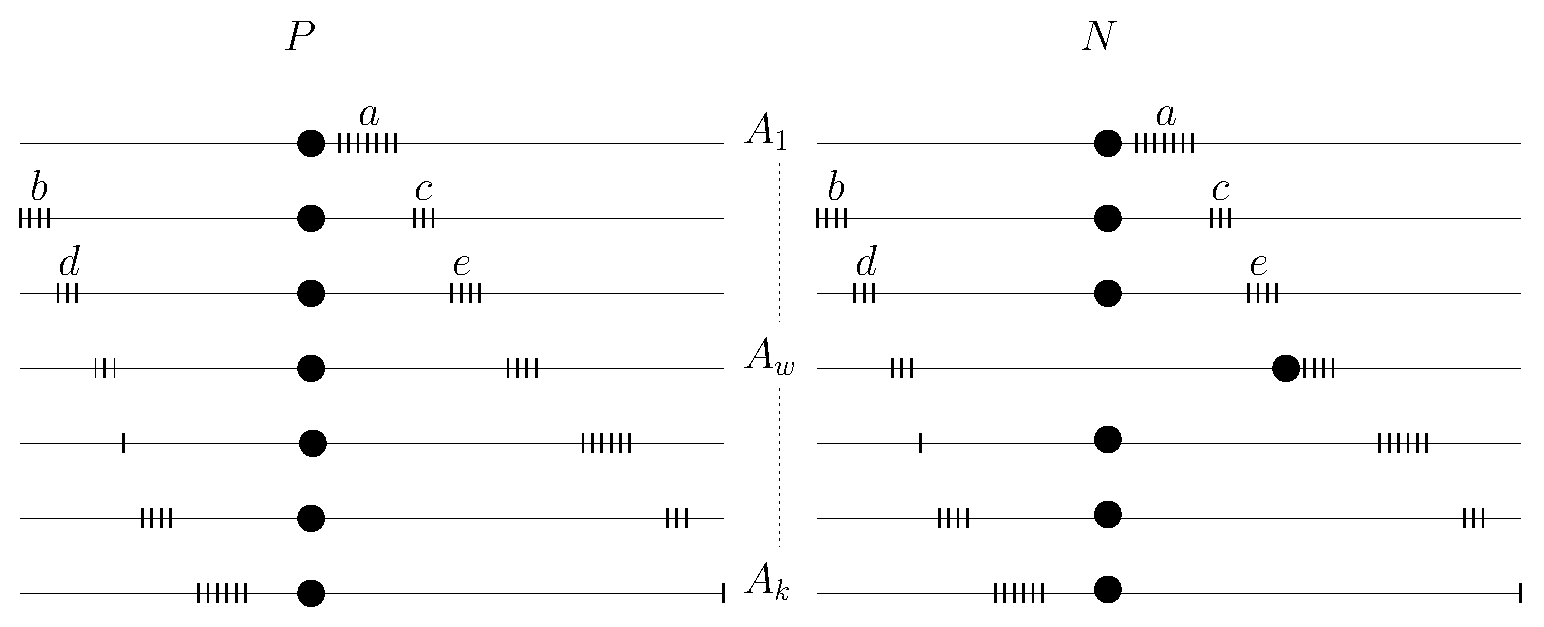
\includegraphics[angle=0,width=12cm]{PNdistribution}}
\caption{Distribution on $(P,N)$: each element of value $v$ is
represented by a dot of x-coordinate $v$, and large dots correspond to
the element at position $p_i$ in each array
$A_i$. \label{fig:PandNdistribution}}
\end{figure}

Let $x=A_1[1]$ be the first element of the first array.
%
Define $x$-comparisons to be the comparisons between any element and $x$.
%
Because of the special relative positions of the elements, a
comparison between two elements $b$ and $d$ in any arrays does not
yield more information than the two comparisons between $x$ and $b$
and between $x$ and $d$: the positions of elements $b$ and $d$
relative to $x$ permit to deduce their order.
%
Hence any algorithm performing $C$ comparisons between arbitrary
elements can be expressed as an algorithm performing no more than $2C$
$x$-comparisons, and any lower bound $L$ on the complexity of
algorithms using only $x$-comparisons is an $L/2$ lower bound on the
complexity of algorithms using comparisons between arbitrary elements.

The alternation of such instances is at most $4$, and the redundancy
of such instances is no more than $3+{1/(k{-}1)}$, which is less
than $4$:
%
\begin{itemize}
\item the interval $\left(-\infty,A_{1}[1]\right)$ is sufficient to
  certify that no element smaller than $x$ is in the intersection, and
  stands for a redundancy of at most $1$;
%
\item the interval $\left(A_{1}[n_1],+\infty,\right)$ is sufficient to
  certify that no element larger than $A_{1}[n_1]$ is in the
  intersection, and stands for a redundancy of at most $1$;
%
\item  the interval $\left[A_1[1],A_{1}[n_{1}]\right]$ is sufficient in $N$
to complete the partition-certificate, and stands for a redundancy of
at most $1$;
% 
\item  the singleton $\{x\}$ and the interval
$\left(A_1[1],A_{1}[n_{1}]\right]$ are sufficient in $P$ to complete
the partition-certificate, and stand for a redundancy of at most
$1{+}{1/(k-1)}$.
\end{itemize}

The only difference between instances $P$ and $N$ is the relative
position of the element $A_{w}[p_{w}]$ to the other elements composing
the instance, as described in Figure~\ref{fig:PandNdistribution}.
%
Any algorithm computing the intersection of $P$ has to find the
$(k-1)$ positions $\{p_2,\ldots,p_k\}$.
%
Any algorithm computing the intersection of $N$ has to find $w$ and
the
associated
position $p_w$.
%
Any algorithm distinguishing between $P$ and $N$ has to find $p_w$:
%
we will prove that it needs on average almost
${F/2}={(1/2)}\sum_{i=2}^k\log_2(2n_i+1)$ $x$-comparisons to do so on
a distribution corresponding to the uniform choice between an instance
$N$ and an instance $P$.

Consider a deterministic algorithm using
only $x$-comparisons to compute the intersection.
%
As the algorithm  has not distinguished between $P$ and $N$ till it
found $w$, let $X_i$ denote the number of $x$-comparisons performed
 in array $A_i$ for both $P$ or $N$.
%
Let $Y_i$ denote the number of $x$-comparisons performed  in
array $A_i$ for $N$;
%
and let $\xi_i$ be the indicator variable which equals $1$ exactly if
$p_i$ has been determined  on instance $P$.
%
The number of comparisons performed  is $C=\sum_{i=2}^k X_i$.
Restricting ourselves to arrays in which the position $p_i$ has been
determined, we can write $C\geq\sum_{i=2}^k X_i\xi_i
=\sum_{i=2}^k Y_i\xi_i$.

Let us consider $E(Y_i\xi_i)$: the expectancy can be decomposed as a
sum of probabilities $E(Y_i\xi_i){=}\sum_h\Pr\{Y_i\xi_i{\geq}h\}$, and
in particular
$E(Y_i\xi_i){\geq}\sum_{h=1}^{F_i}\Pr\{Y_i\xi_i{\geq}h\}$.
%
Those terms can be decomposed using the property
$\Pr\{a{\vee}b\}\leq\Pr\{a\}{+}\Pr\{b\}$:
%$\Pr\{Y_i\xi_i\geq h\}$
\begin{eqnarray}
\Pr \{ Y_i\xi_i\geq h \} 
&  =    & \Pr \{ Y_i\geq h \wedge \xi_i=1 \}   \nonumber\\
&  =    &  1 - \Pr \{ Y_i< h \vee \xi_i=0 \} \nonumber\\
&  \geq &  1 - \Pr \{ Y_i< h \} - \Pr \{ \xi_i=0 \} \nonumber\\
&  =    &  \Pr \{ \xi_i=1 \} -\Pr \{ Y_i< h \} \label{equation1}
\end{eqnarray}

The probability $\Pr\{Y_i<h\}$ is bounded by the usual decision
tree lower bound: if we consider the binary $x$-comparisons performed
 in set $A_i$, there are at most $2^{h}$ leaves at
depth less than $h$.
%
Since the insertion rank of $x$ in $A_i$ is uniformly chosen, these
leaves have the same probability and have total probability at most
$\Pr\{Y_i{<}h\}{\leq}{2^{h}/(2n_i+1)}{=}2^{h-F_i}$.
%
Those terms for $h\in\{1,\ldots,F_i\}$ form a geometric sequence whose
sum is equal to $2(1-2^{-F_i})$,
%
so $E(Y_i\xi_i) \geq F_i \Pr\{\xi_i=1\} - 2(1-2^{-F_i})$.
%
Then 
\begin{eqnarray}
E(C)\geq\sum_{i=2}^k E(Y_i \xi_i)
&\geq& \sum_{i=2}^k F_i \Pr\{\xi_i=1\}
      - \sum_{i=2}^k 2(1-2^{-F_i})
\nonumber\\ 
&\geq& \sum_{i=2}^k F_i \Pr\{\xi_i=1\}
      + 2\sum_{i=2}^k 2^{-F_i}  - 2(k-2).
\label{equation2}
\end{eqnarray}


Let us fix $p=(p_2, \ldots,p_k)$.
%
There are only $k-1$ possible choices for $w$.
%
The algorithm can only differentiate between $P$ and $N$ when it finds
$w$.
%
Let $\sigma$ denote the order in which these instances are dealt with
for $p$ fixed.
%
Then $\xi_i=1$ if and only if $\sigma_i\leq\sigma_w$, and so
 $\Pr\{\xi_i=1|p\}=\sum_{j:\sigma_j\geq\sigma_i}{F_j /  F}$.

Summing over $p$, and then over $i$, we get an expression of the first term in
Equation~(\ref{equation2}):
$$
\Pr\{ \xi_i=1 \} 
= \sum_{p} 
        \Pr \{ \xi_i=1 | p\} 
	\Pr \{ p\} 
= \sum_{p} 
	\sum_{j: \sigma_j \geq\sigma_i}
		{ F_j\over F} \Pr \{ p\} 
$$
$$
\sum_{i=2}^k F_i \Pr\{\xi_i =1\} 
=  \sum_{p} \sum_{i=2}^k \sum_{j : \sigma_j \geq \sigma_i }
	   { F_i F_j \over F}  \Pr \{ p\}
=  \sum_{p} \Pr \{ p\}
       \sum_{i=2}^k \sum_{j : \sigma_j \geq \sigma_i }
       \frac   {F_i F_j}
	       {F}.   		
$$
%
In the sum, each term ``$F_i F_j$'' appears exactly once,
and 
$$\left(\sum_i F_i\right)^2
=2\sum_i\sum_{i\leq j} F_i F_j - \sum_i {F_i}^2,$$ hence
 $$ \sum_{i=2}^k \sum_{j : \sigma_j \geq \sigma_i }  F_i F_j  
=\frac{1}{2} \left( 
\left( \sum_{i=2}^k F_i \right)^2 +  \sum_{i=2}^k {F_i}^2 
\right),$$
which is independent of $p$.
%
Then we can conclude:
$$
\sum_{i=2}^k F_i \Pr \{\xi_i=1\} 
= \frac{1}{2} \frac{1}{F}
     \left( \left(\sum_{i=2}^k F_i\right)^2 + \sum_{i=2}^k {F_i}^2 \right) 
     \sum_{p}\Pr\{p\}\\
%&\geq& \frac{1}{2} \frac{1}{F} \left(\sum_{i=2}^k F_i\right)^2\\
= \frac{1}{2} \sum_{i=2}^k F_i .
$$ 
%
Plugging this into Equation~(\ref{equation2}), we obtain a lower bound
on the average number of $x$-comparisons $E(C)$ performed by any
deterministic algorithm which performs only $x$-comparisons, of
$(1/2)\sum_{i=2}^k F_i+2\sum_{i=2}^k 2^{-F_i}-2(k{-}2)$, which
is equal to $(1/2)\sum_{i=2}^k\log_2(2n_i{+}1) + 2\sum_{i=2}^k {1/(2n_i{+}1)} - 2(k{-}2)$.
%
This  implies a lower bound of 
${(1/4)}\sum_{i=2}^k\log_2(2n_i{+}1) + \sum_{i=2}^k {1/(2n_i{+}1)} - (k{-}2)$ 
%
on the average number of comparisons performed by
{\em any} deterministic algorithm, hence the result.
\qed\end{proof}

%
\begin{lemma}\label{lem:generaldistribution}
For any $k\geq 2$, $0{<}n_1{\leq}\ldots{\leq}n_k$ and
$\rho{\in}\{4,\ldots,4n_1\}$, there is a distribution on instances of
the intersection problem of signature at most $(k,n_1,\ldots,n_k)$, of
alternation and redundancy at most $\rho$, such that any deterministic
algorithm performs on average $\Omega(\rho \sum_{i=1}^k \log(n_i/\rho))$ comparisons.
\end{lemma}
\begin{proof}
Let's draw $p{=}\lfloor\rho/4\rfloor$ pairs
$(P_j,N_j)_{j\in\{1,\ldots,p\}}$ of sub-instances of signature
$(k,\lfloor n_1/p\rfloor,\ldots,$ $\lfloor n_k/p\rfloor)$ from
the distribution of Lemma~\ref{lem:elementproblem}.
%
As $\rho\leq4n_1$, $p\leq n_1$ and $\lfloor n_1/p\rfloor>0$, the sizes
of all the arrays are positive.
%
Let's choose uniformly at random each sub-instance $I_j$ between the
sub-instance $P_j$ which intersection is a singleton and the
sub-instance $N_j$ which intersection is empty, and form a
larger instance $I$ by unifying the arrays of same index from each
sub-instance, such that the elements from two different sub-instances
never interleave, as in Figure~\ref{fig:generaldistribution}.
\begin{figure}
\centerline{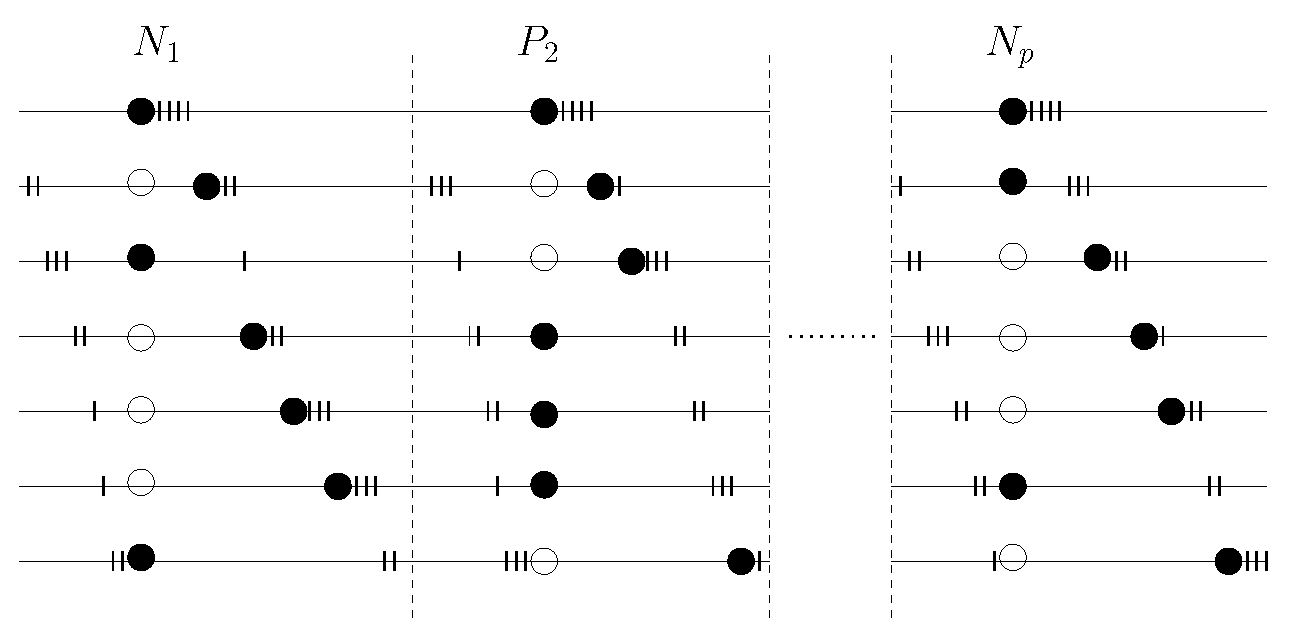
\includegraphics[angle=0,width=8cm]{generaldistribution.eps}}
\caption{$p$ elementary instances unified to form a single large instance.}\label{fig:generaldistribution}
\end{figure}

This defines a distribution on instances of alternation and redundancy
at most $\rho$ (as $4p=4\lfloor\rho/4\rfloor\leq\rho$), and of
signature at most $(k,n_1,\ldots,n_k)$.
%
Solving this instance implies to solve all the $p$ sub-instances.
Lemma~\ref{lem:elementproblem} gives a lower bound of
$(1/4)\sum_{i=2}^k\log (2n_i/p+1)+\sum_{i=2}^k{1/(2n_i{+}1)}-k{+}2$
comparisons on average for each of the $p$ sub problems, hence a lower
bound of
%
$$(p/4)
  \sum_{i=2}^k   \log(2n_i/p+1)  
               +p\left( \sum_{i=2}^k { 1 / (2n_i/p{+}1) }
                                 -k{+}2
                 \right)
,$$
%
which is $\Omega(\rho\sum_{i=1}^k\log (n_i/\rho))$.  \qed\end{proof}
%


\subsubsection{Application to Alternation}
\label{sec:appl-altern}


Indeed, among instances of same signature and alternation, it is
possible to prove a tight bound on the randomized complexity of the
intersection problem: by providing a difficult distribution of
instances and using the minimax principle, we prove a lower bound on
the complexity of any randomized algorithm solving the
problem~\cite{adaptiveIntersectionAndTThresholdProblems}.
%
\begin{theorem}[Alternation Lower Bound~\cite{adaptiveIntersectionAndTThresholdProblems}]\label{th:alternationLB}
For any $k{\geq} 2$, $0{<}n_1{\leq}\ldots{\leq}n_k$ and
$\delta{\in}\{4,\ldots,4n_1\}$,
%
and for any randomized algorithm $A_R$ for the intersection problem,
%
there is an instance of signature at most $(k,n_1,\ldots,n_k)$ and
alternation at most $\delta$,
%
such that $A_R$ performs $\Omega(\delta\sum_{i=1}^k\log(n_i/\delta))$
comparisons on average on it.
\end{theorem}
\begin{proof}
This is a simple application of Lemma~\ref{lem:generaldistribution}
(stated and proved in Section~\ref{sec:lowerbound})
and of the Yao-von Neumann principle \cite{vonneumann1944,sion58,yao}:
\begin{itemize}
\item Lemma~\ref{lem:generaldistribution} gives a distribution for
$\delta\in\{4,\ldots,4n_1\}$ on instances of
alternation {\em at most} $\delta$,
\item Then the Yao-von Neumann principle permits to deduce from this
distribution a lower bound on the worst case complexity of randomized
algorithms.  \qed\end{itemize}
\end{proof}

On the other hand, the simple deterministic algorithm of
Section~\ref{sec:alternation} reaches this lower bound.
%
As the class of deterministic algorithms is contained in the class of
randomized algorithms, this proves that the bound for the alternation
analysis is tight for randomized algorithms.
%



\subsubsection{Application to Redundancy}
\label{sec:appl-redund}





\begin{theorem}[Redundancy Lower Bound~\cite{optimalityOfRandomizedAlgorithmsForTheIntersectionProblem}]\label{th:standalonelowerbound} \label{th:redundancyLB}
For any $k\geq 2$, $0{<}n_1{\leq}\ldots{\leq}n_k$ and
$\rho\in\{4,\ldots,4n_1\}$, 
%
and for any randomized algorithm $A_R$ for the intersection problem,
%
there is an instance of signature at most $(k,n_1,\ldots,n_k)$, and
redundancy at most $\rho$,
%
such that $A_R$ performs $\Omega(\rho\sum_{i=1}^k\log(n_i/\rho))$
comparisons on average on it.
\end{theorem}

\begin{proof}
The proof is identical to the proof of Theorem~\ref{th:alternationLB},
as the instances generated by the proof are of alternation equal to
their redundancy.
%
This is a simple application of Lemma~\ref{lem:generaldistribution} and
of the Yao-von Neumann principle \cite{vonneumann1944,sion58,yao}:
\begin{itemize}
\item Lemma~\ref{lem:generaldistribution} gives a distribution for
$\rho\in\{4,\ldots,4n_1\}$ on instances of redundancy {\em at most}
$\rho$, 
\item Then the Yao-von Neumann principle permits to deduce from this
distribution a lower bound on the worst case complexity of randomized
algorithms.  \qed\end{itemize}
\end{proof}


This analysis is more precise than the lower bound previously
presented~\cite{adaptiveIntersectionAndTThresholdProblems}, where the
additive term in $-k$ was ignored, although it makes the lower bound
trivially negative for large values of the difficulty $\delta$.
%
Here the additive term is suppressed for $\min_i n_i\geq128$, and the
multiplicative factor between the lower bound and the upper bound is
reduced to $16$ instead of $64$.
%
This technique can be applied to the alternation analysis of the
intersection with the same result.
%
Note also that a multiplicative factor of $2$ in the gap comes from
the unbounded searches in the algorithm, and can be reduced using a
more complicated algorithm for the unbounded
search~\cite{anAlmostOptimalAlgorithmForUnboundedSearching}.



One could wonder how the lower bound evolves for redundancy values
larger than $4n_1$.
%
The following result shows that no instance with such redundancy can
exist.
%
\begin{lemma}\label{lem:rhoupperbound}
For any $k\geq 2$ and
$0{<}n_1{\leq}\ldots{\leq}n_k$, any instance of signature
$(k,n_1,\ldots,n_k)$ has redundancy $\rho$ at most $2n_1{+}1$.
\end{lemma}
\begin{proof}
First observe that there is always a partition-certificate of size
$2n_1+1$. Then that the redundancy of any partition-certificate is by
definition smaller than the size of the partition. Hence the result.
\qed\end{proof} 
%
Note that this does not contradict the result from
Lemma~\ref{lem:generaldistribution}, which defines a distribution of
instances of redundancy {\em at most} $4n_1$.

\subsection{Comparisons between the analysis}\label{sec:comparison}

The redundancy analysis is strictly finer than the alternation analysis:
%
some algorithms, optimal for the alternation analysis, are not optimal
anymore in the redundancy analysis (Theorem~\ref{th:finer}),
%
and any algorithm optimal in the redundancy analysis is optimal in the
alternation analysis (Theorem~\ref{th:strictlyfiner}).
%
So the {\tt Rand Intersection} algorithm is theoretically better than
its deterministic variant in the comparison model, and the redundancy
analysis permits a better analysis than the alternation analysis.

%
\begin{theorem}\label{th:finer}
For any $k\geq 2$, $0{<}n_1{\leq}\ldots{\leq}n_k$ and
$\rho\in\{4,\ldots,4n_1\}$, 
%
and for any deterministic algorithm for the intersection problem,
%
there is an instance of signature at most $(k,n_1,\ldots,n_k)$, and
redundancy at most $\rho$,
%
such that this algorithm performs $\Omega(k\rho\sum_i\log(n_i/k\rho))$
comparisons on it.
\end{theorem}
\begin{proof}
The proof uses the same decomposition than the proof of
Theorem~\ref{th:standalonelowerbound}, but uses an adversary argument
to obtain a deterministic lower bound.
%
Build $\delta={k\rho/3}$ sub-instances of signature
$(k,\lfloor{n_1/\delta}\rfloor,\ldots,\lfloor{n_k/\delta}\rfloor)$,
redundancy at most $3$, such that $x=A_1[1]$ is present in
roughly half of the other arrays, as in
Figure~\ref{fig:halffullsubinstance}.



On each sub-instance an adversary can force any deterministic algorithm
to perform a search in each of the arrays containing $x$, and in a
single array which does not contain $x$.
%
Then the deterministic algorithm performs
$(1/2)\sum_{i=2}^k\log{(n_i/\delta)}$ comparisons for each
sub-instance.
%
\begin{figure}
\hfill
\begin{minipage}{0.33\textwidth}
\centerline{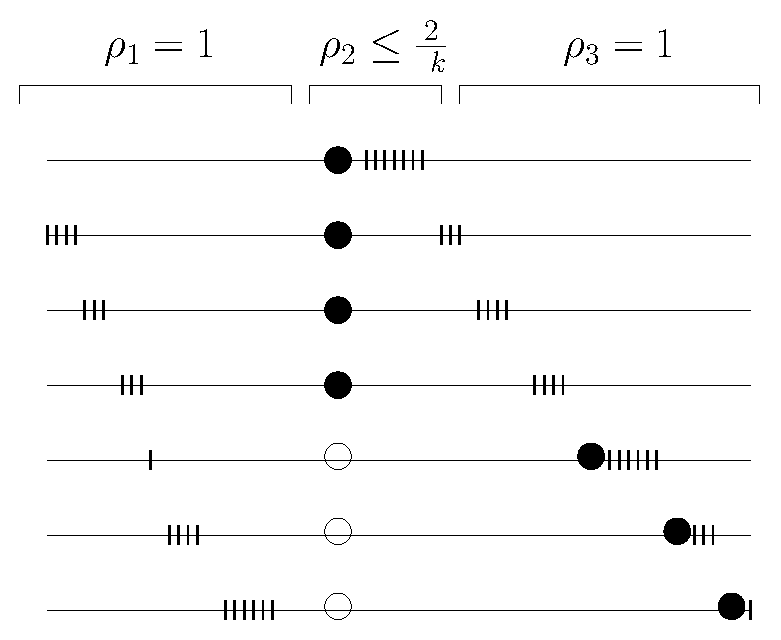
\includegraphics[angle=0,height=3.3cm]{halffullsubinstance.eps}}
\caption{Element $x$ is present in half of the arrays of the sub-instance.\label{fig:halffullsubinstance}
}
\end{minipage}
\hfill
\begin{minipage}{0.66\textwidth}
\centerline{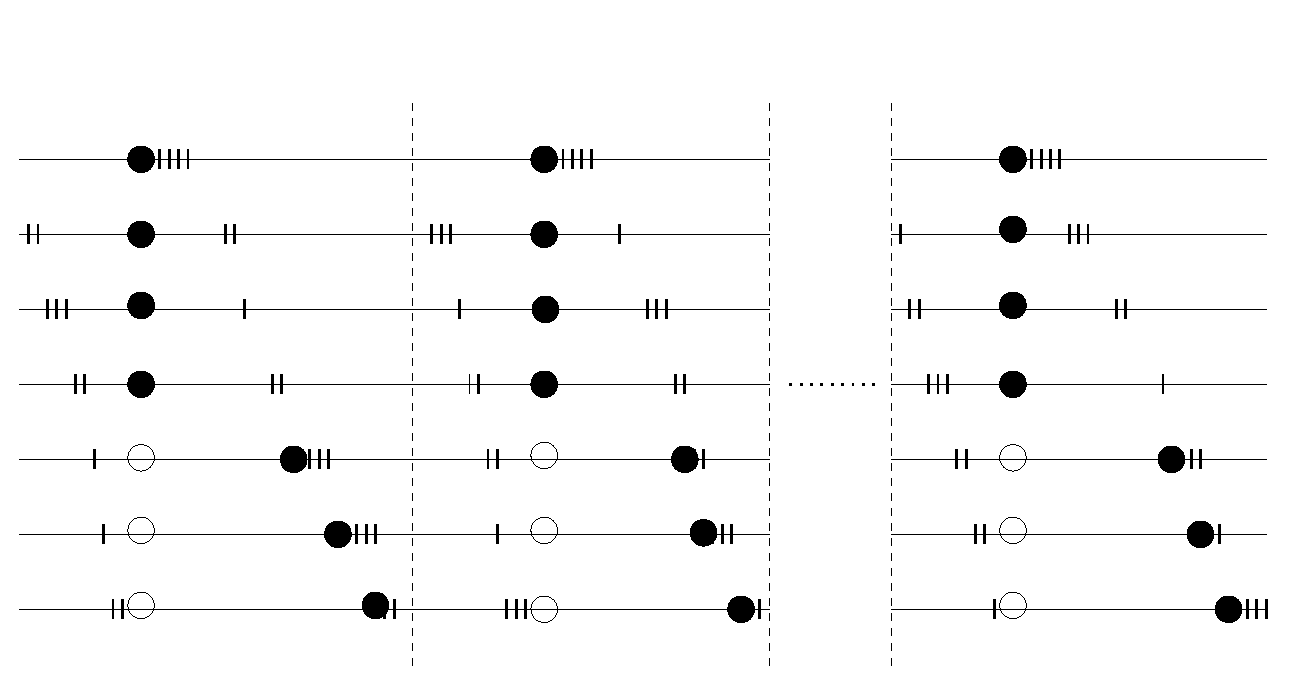
\includegraphics[angle=0,height=3.5cm]{halffullinstance.eps}}
\caption{The adversary performs several strategies in parallel, one
for each
sub-instance. \label{fig:halffullinstance}}\end{minipage}\hfill \hfill
\hfill \hfill
\end{figure}
%
In total over all sub-instances, the adversary can force any
deterministic algorithm to perform
${(\delta/2)}\sum_{i=2}^k\log{(n_i/\delta)}$ comparisons, i.e.
${(k\rho/4)}\sum_{i=2}^k\log{(n_i/k\rho)}$, which is
$\Omega({k\rho}\sum_{i=2}^k\log{(n_i/k\rho)})$.
\qed\end{proof}
%
As $x\log(n/x)$ is a function increasing with $x$,
$k\rho\sum_i\log(n_i/k\rho)$ is several times larger than the lower
bound $\rho\sum_i\log(n_i/\rho)$, hence no deterministic algorithm can
be optimal in the redundancy analysis.
%
\begin{theorem}\label{th:strictlyfiner}
Any algorithm optimal in the redundancy analysis is optimal in the
alternation analysis.
\end{theorem}
\begin{proof}
By definition of the redundancy $\rho$ and of the alternation $\delta$
of an instance, $\rho\leq\delta$.
%
So if an algorithm performs $O(\rho\sum \log{n_i/\rho})$
comparisons, it also performs $O(\delta\sum\log{n_i/\delta})$
comparisons.
%
Hence the result, as this is the lower bound in the alternation analysis.
\qed\end{proof}


This proves also that the measure of difficulty of
Demaine~\etal~\cite{dlm} is not comparable with the measure of
redundancy, as it is not comparable with the measure of
alternation~\cite[Section~2.3]{deterministicAlgorithmForTheTThresholdSetProblem}.
%
This means that the two measures are complementary, without being
redundant in any way, as it was for the alternation.
%
All those measures describe the difficulty of the instance:
\begin{itemize}
\item the {\em alternation}~\cite[Section~2.3]{deterministicAlgorithmForTheTThresholdSetProblem}
describes the number of key blocks of consecutive elements in the
instance;
\item the {\em gap cost}~\cite{dlm} describes the repartition of the
size of those blocks;
\item the {\em
redundancy}~\cite{optimalityOfRandomizedAlgorithmsForTheIntersectionProblem}
describes the difficulty to find each
block.
\end{itemize}
%
But only the {\em gap cost} and the {\em redundancy} matter, because the
alternation analysis is reduced to the redundancy analysis.



\section{Weighted $t$-Threshold Set}
\label{sec:t-threshold-set}



Conjunctive queries are well known. Indeed, most search engines
implement them.
% 
Given a list of labels (e.g.  keywords), the answer consists of all
the objects (e.g. webpage references) which are associated with all of
the labels.
%
Given an index such as described in the section above, solving a
conjunctive query composed of $\nbkeywords$ labels implies computing
the intersection of $\nbkeywords$ rows in a binary relation, which is
a well studied
problem~\cite{aFastSetIntersectionAlgorithmForSortedSequences,experimentalAnalysisOfAFastIntersectionAlgorithmForSortedSequences,dlm,dlmAlenex}


As an empty intersection can be an uninformative answer to a
conjunctive query, we should consider other approaches. 
%
Researchers in information retrieval suggest a number of ways to deal
with this problem.
%
For example, one can relax both queries and document index in a number
of different ways that are summarized by Bordogna and
Pasi~\cite{DBLP:conf/essir/BordognaP00}.
%
Barbay and Kenyon~\cite{adaptiveIntersectionAndTThresholdProblems}
proposed the adaptive algorithm to answer the query where for a given
parameter $\threshold$ the answer consists of the references matching
at least $\threshold$ of the $\nbkeywords$ labels composing the query.
%
Given an index such as described in the section above, solving this
new type of query implies computing the {\em threshold set} of 
$\nbkeywords$ rows in a binary relation, the set of objects associated
with at least $\threshold$ labels among the $\nbkeywords$ specified.

Barbay and Veraskouski
\cite{adaptiveAlgorithmsForWeightedQueriesOnWeightedBinaryRelationsAndLabeledTrees}
extended further this type of query to {\em weighted threshold}
queries, by considering
%
weighted queries $\Q:[\nblabels]\rightarrow\{0,\ldots,\maxWeightQ\}$,
where $\nblabels$ is the number of admissible keywords, and
%
weighted binary relations 
$\R:[\nblabels]\times[\nbobjects]\rightarrow\{0,\ldots,\maxWeightR\}$
~\footnote{By $[m]$ we denote $\{1, \ldots, m\}$ for any integer number $m$.}.
%
The {\em score} of an object $\objectx$ relative to a query $\Q$ on a
relation $\R$ is then defined as the linear combination of those
weights, i.e. $\score(\R,\Q,\objectx) = \sum_{\labelx \in
  [\nblabels]}{\Q(\labelx)\R(\labelx,\objectx)}$, that corresponds to
the notion of the {\em Retrieval Status Value} (or RSV) described by
Bordogna and Pasi~\cite{DBLP:conf/essir/BordognaP00}.
%
The answer to a query with parameter $\threshold$ is the set of
objects with score at least~$\threshold$: this definition matches the
original one from Barbay and Kenyon when each weight is either null or
unitary (the {\em unweighted} case).

We define the {\em alternation} of a weighted threshold set instance
as the size $\difficulty$ of the smallest possible
partition-certificate of the instance.
%
\begin{LONG}
  The alternation is related to the {\em non-deterministic} complexity
  of the instance, as it corresponds to the complexity of a
  non-deterministic algorithm which would produce the shortest
  partition-certificate of the instance.
\end{LONG}
% 
In the unweighted case (where all weights are unitary), if no object
match the query then the alternation is exactly the non-deterministic
complexity of the instance, i.e. the complexity of the best
non-deterministic algorithm checking the answer to the query.

\begin{figure}
  \centering
$$  \begin{array}[b]{cc|c|c|c|c|c|c|cccc|ccccc|cccccc|cccccccc}

    & 
    \multicolumn{7}{}  											                         &                    & & &
 1  &  2 &  3 &  4 &  5 &  6 &  7 & 8  &  9 &  10 &  11 & 12 &  13 &  14 & 15 & 16  & 17 & 18  &      &    
\\ \cline{3-8} \cline{11-28}


    \mbox{Music} & \rightarrow      
& 1                                & 8       & 10      & 12           & 15      & 17                 & & \rightarrow &
  1  &  . &  . &  . &  . &  . &  . & 1  &  . &  1 &  . &  1 &  . &  . &  1 &  . &  1 &  .  &   &    
\\ \cline{3-8}
    \mbox{Jazz} & \rightarrow
    & 2       & 4       & 6            & 9       & 11      & 13                                      & & \rightarrow &
  . & 1  &  . & 1  &  . & 1  &  . &  . & 1  &  . &  1 &  . &  1 &  . &  . &  . &  . &  . &     &    
\\ \cline{3-8}
    \mbox{Rock} & \rightarrow      
         & 3       & 5       & 7                                & 14      & 16      & 18             & & \rightarrow &
  . &  . & 1  &  . & 1  & .  & 1  &  . &  . &  . &  . &  . &  . &  1 &  . &  1 &  . &  1 &    
\\ \cline{3-8}
  \end{array}$$
  \begin{minipage}{.9\linewidth}
    \caption{ An example of how a conjunctive query composed 
      of three keywords corresponds to the
      intersection of the three corresponding sets.  
      % 
      The alternation of the instance is $\difficulty=4$, 
      the number of intervals of a partition certificate 
      where each interval has an empty intersection with at least one of the sets.
      % 
      Barbay and Kenyon's algorithm performs
      $7{\leq}\difficulty\nbkeywords{=}12$ searches (for the numbers
      $1,2,3,8,9,14,15$).  \label{fig:sequentialExample} }
  \end{minipage}
\end{figure}

Barbay and Kenyon~\cite{adaptiveIntersectionAndTThresholdProblems}
proved that any randomized algorithm performs
$\Omega(\difficulty\nbkeywords)$ searches in the worst case over
instances of difficulty $\difficulty$ on $\nbkeywords$ labels, and
proposed an optimal deterministic algorithm for the unweighted case on
sorted arrays.
%
We analyze the complexity of the algorithms in terms of search and
priority queue operations, where a priority queue operation is either an insertion or a
deletion from a priority queue, and where each search operation is a search for
the particular object in a data structure representing an ordered list
of objects.
%
We propose an optimal algorithm for the weighted case with any data
structure supporting the search for the insertion rank in an indexed
set:

\begin{theorem}\label{th:threshold-set}
  Consider a weighted binary relation
  $\R:[\nblabels]\times[\nbobjects]\rightarrow\{0,\ldots,\maxWeightR\}$,
  a weighted query
  $\Q:[\nblabels]\rightarrow\{0,\ldots,\maxWeightQ\}$, and a
  non-negative integer $\threshold$.
  % 
  There is an algorithm that computes the threshold set for $\Q$ on
  $\R$ with threshold-value of $\threshold$ in $\bigo(\difficulty\nbkeywords)$
  search and priority queue operations, where
  % 
  $\difficulty$ is the alternation of the instance and
  % 
  $\nbkeywords$ is the number of labels of positive weight in~$\Q$.
\end{theorem}

  \begin{algorithm}
    \centering
    \caption{Algorithm  answering Threshold Set queries }
    \label{alg:ThresholdOnBinRel}
    \begin{algorithmic}
      \STATE Set $\objectx$ to $-\infty$, 
      $\setNO$ and $\setYES$ to $\emptyset$
      and $\setMAYBE$ to the set of all labels of non-null weight;

      \STATE \idtt{Update}$(\objectx,\setYES,\setNO,\setMAYBE,\scoremin,\scoremax)$ 
      using Algorithm~\ref{alg:choiceBR};

      \WHILE{$\objectx<\infty$}

        \STATE Set $\labelx$ to the next label from $\setMAYBE$ in round
        robin order, and deduct $\maxWeightR\Q(\labelx)$ from
        $\scoremax$;

        \STATE Search for the insertion rank of $\objectx$ among the
        objects labeled $\labelx$;

        \IF{$\objectx$ is associated with a label $\labelx$}
          \STATE Move $\labelx$ from $\setMAYBE$ to $\setYES$;
          \STATE Add $\Q(\labelx)\R(\labelx,\objectx)$ to
          $\scoremin$ and $\scoremax$;
          \STATE {\bf if} {$\threshold\leq\scoremin$} 
                 {\bf then } Output $\objectx$;
        \ELSE    
          \STATE Move $\labelx$ from $\setMAYBE$ to $\setNO$;
        \ENDIF

        \IF{$\threshold \le \scoremin$ or $\threshold>\scoremax$}
           \STATE \idtt{Update}$(\objectx,\setYES,\setNO,\setMAYBE,\scoremin,\scoremax)$;
        \ENDIF

      \ENDWHILE
    \end{algorithmic}
  \end{algorithm}

  \begin{PROOF}
    \begin{proof}[of Theorem~\ref{th:threshold-set}]
      Consider the steps of Algorithm~\ref{alg:ThresholdOnBinRel}:
      given a query $\Q$ with $\nbkeywords$ positive weights and a
      threshold-value $\threshold$, the algorithm computes the set of
      objects scoring at least $\threshold$ for a weighted binary
      relation $\R$ associating objects with labels.

      Our algorithm goes through a number of phases. At each phase it
      considers one object $\objectx$, in increasing order, and bounds
      its score by an interval $[\scoremin,\scoremax]$.
  %
      The algorithm can decide whether $\objectx$ belongs to the
      result set through this interval and without computing the
      object's exact score
      ($\threshold\leq\scoremin\leq\score(\objectx)$).
  % 
      On the other hand, if for a given interval of consecutive
      objects there is a set of labels not associated with any of them
      with large total weight, this interval certifies that none of
      those objects belongs to the result set
      ($\score(\objectx)\leq\scoremax<\threshold$).
  % 
      The key issue of the algorithm is the choice of the values of
      $\objectx$ and of the labels to consider.

      This choice is described in Algorithm~\ref{alg:choiceBR}, which
      is based on the decomposition of the set of labels of positive
      weights in three disjoint sets: $\setYES$, $\setMAYBE$ and
      $\setNO$:
  %
      \begin{itemize}
      \item $\setYES$ corresponds to the labels already known to be
        associated with the current value of $\objectx$. It can be
        implemented as a simple set, for instance in an array.
      \item $\setMAYBE$ corresponds to the labels which could be
        associated with the current value of $\objectx$. It is
        implemented as a FIFO queue so that each label in it is
        considered equally often.
      \item $\setNO$ corresponds to the labels which are known not to
        be associated with the current value of $\objectx$. It is
        implemented as a priority queue of at most $\nbkeywords$
        elements, and the labels $\labelx$ it contains are ordered by
        the value of the first object larger than $\objectx$
        associated with label $\labelx$.
      \end{itemize}
  % 
      The values of the bounds $\scoremin$ and $\scoremax$ on the
      potential score of $\objectx$ are direct consequences of those
      definitions: $\scoremin$ depends on the weights of the labels in
      $\setYES$, i.e.
      $\scoremin=\sum_{\labelx\in\setYES}\Q(\labelx)\R(\labelx,\objectx)$;
      and $\scoremax$ adds the maximum potential weights of the labels
      in $\setMAYBE$ to $\scoremin$, i.e.
      $\scoremax=\scoremin+\sum_{\labelx\in\setMAYBE}\Q(\labelx)\maxWeightR$.

      To choose a new value for $\objectx$, the algorithm removes
      labels from the set $\setMAYBE$ till it reaches a critical
      weight, where removing any other label would make it impossible
      for an object matching only the labels of $\setMAYBE$ to score
      above the threshold.
  % 
      Then, the smallest object potentially in the result set
      corresponds to the first label of the priority queue
      implementing set $\setNO$.
 

      %%%%%%%%%%%%%%%%%% ADAPTIVE
      %%%%%%%%%%%%%%%%%% ANALYSIS %%%%%%%%%%%%%%%%%%%%%%%%%%%%%%%%%%%%%%%%%

      Consider a phase of the execution where the algorithm is
      processing an interval of the partition-certificate consisting
      of only one object $\objectx$.
      Algorithm~\ref{alg:ThresholdOnBinRel} performs at most
      $\nbkeywords$ iterations of the main loop to decide whether
      $\objectx$ has enough score or not without updating $\objectx$
      (through Algorithm~\ref{alg:choiceBR}). Once the decision about
      $\objectx$ is made, the algorithm updates $\objectx$ and moves
      to the next phase. Updating of $\objectx$ takes not more than
      $\nbkeywords$ loop iterations of Algorithm~\ref{alg:choiceBR}.
      Thus during each phase, the algorithm performs at most
      $\bigo(\nbkeywords)$ search and priority queue operations.

      Consider a phase corresponding to the interval of the
      partition-certificate that does not have any objects with enough
      score and a subset $S$ of labels that are not associated with
      any of the objects in this interval.
      Algorithm~\ref{alg:ThresholdOnBinRel} may update $\objectx$ more
      than once during the same phase. We prove the upper bound on the
      number of operations through considering the way the algorithm
      moves labels from one set to another.
  
      The only way Algorithm~\ref{alg:ThresholdOnBinRel} moves labels
      is from set $\setMAYBE$ to either set $\setYES$ or set $\setNO$.
      Algorithm~\ref{alg:choiceBR}, on the other hand, move labels
      from $\setYES$ to $\setMAYBE$, from $\setMAYBE$ to $\setNO$, and
      from $\setNO$ to $\setYES$ in this order. As it cannot move
      labels that are in $S$ to $\setYES$, the algorithm has the only
      possible loop $\setMAYBE \longrightarrow \setNO \longrightarrow
      \setYES \longrightarrow \setMAYBE$ for these labels.
  
      However, the algorithm does not move any labels from $S$ that it
      already moved to $\setNO$ during the processing of the same
      interval, because the label's successor is out of the current
      interval and cannot be processed in the current phase. While the
      algorithm retrieves labels from set $\setMAYBE$ in round-robin
      order, it cannot retrieve any label from set $\setMAYBE$ for the
      second time until all the labels from subset $S$ appear in set
      $\setNO$, which effectively means that the next element
      $\objectx$ will be outside of the interval and the algorithm
      proceeds to the new phase. While it takes a constant time for
      the algorithm to move each label from set $\setMAYBE$ back to
      set $\setMAYBE$, it needs $\bigo(\nbkeywords)$ search and
      priority queue operations to complete this phase.
  
      As the algorithm spends $\bigo(\nbkeywords)$ to complete any
      phase, and any instance has $\difficulty$ intervals that
      correspond to $\difficulty$ phases, the total complexity of the
      algorithm is $\bigo(\difficulty \nbkeywords)$.  \qed
    \end{proof}
  \end{PROOF}
      \begin{algorithm}
        \begin{algorithmic}
          \caption{\idtt{Update}$(\objectx,\setYES,\setNO,\setMAYBE,\scoremin,\scoremax)$}
          \label{alg:choiceBR}
 
          \STATE Add all the labels from $\setYES$ to the set
          $\setMAYBE$ and set $\scoremax$ to
          $\sum_{\labelx\in\setMAYBE}\Q(\labelx)\maxWeightR$; \STATE
          Choose a label $\labelx$ in round-robin order from
          $\setMAYBE$;

          \WHILE{$\scoremax-\Q(\labelx)\maxWeightR \ge \threshold$}
          \STATE Deduct $\Q(\labelx)\maxWeightR$ from $\scoremax$, and
          move $\labelx$ from $\setMAYBE$ to $\setNO$; \STATE Choose a
          label $\labelx$ in round-robin order from $\setMAYBE$;
          \ENDWHILE

          \STATE Find the subset $S\subset\setNO$ of labels $\labelx$
          such that the successor of $\objectx$ among the objects
          labeled $\labelx$ is minimal;

          \STATE Move all the labels of $S$ from $\setNO$ to
          $\setYES$, and set $\scoremin$ to
          $\sum_{\labelx\in\setYES}\Q(\labelx)\R(\labelx,\objectx)$;
      
          \STATE Update $\objectx$ to its successor among the objects
          labeled $\labelx$, for any label in $\setYES$;
        \end{algorithmic}
      \end{algorithm}

  Note that $\nbkeywords$ is the number of labels with a positive weight.
  % 
  If the binary relation is implemented by postings lists, and the
  priority queue is implemented using a heap, the complexity of the
  algorithm is $\bigo ( \difficulty \nbkeywords \lg (n / (\difficulty
  \nbkeywords)) + \difficulty \nbkeywords \lg {\nbkeywords } )$, where
  $n$ is the sum of the sizes of all postings lists and $\nbkeywords$
  is the maximum size of the priority queue.
  % 
  If the binary relation is implemented using
  Barbay~\etal's~\cite{weightedQueriesOnBinaryRelationsAndMultiLabeledTrees}
  succinct encoding and the priority queue is implemented using
  Andersson and
  Thorup's~\cite{tighterWorstCaseBoundsOnDynamicSearchingAndPriorityQueues}
  structure, the complexity of the algorithm is
  $\bigo(\difficulty\nbkeywords\lg\lg\nblabels +
  \difficulty\nbkeywords(\lg\lg\nbkeywords)^2)$ in the RAM model with
  word size $\Theta(\lg\max\{\nblabels,\nbobjects\})$.













\section{Perspectives}
\label{sec:perspectives}


The $t$-threshold set and opt-threshold set
problems~\cite{deterministicAlgorithmForTheTThresholdSetProblem} are
natural generalizations of the intersection problem, which could be
useful in indexed search engines.
%
The redundancy seems to be important in the complexity of these
problems as well, but a proper measure is harder to define in this
context.
%
As similar techniques are applied to solve queries on semi-structured
documents~\cite{indexTreesForDescendantTreeQueriesInTheComparisonModel},
the redundancy could be useful in this domain too, but the definition
of the proper measure of difficulty is even more evasive in this
context.
%
More generally, the set operations are combined in practice in a
recursive way, forming Union/Intersection trees.
%
Farzan~\etal~\cite{worstCaseOptimalUnionIntersectionExpressionEvaluation}
studied the non-adaptive complexity of the evaluation of such
expressions: the adaptive analysis of such a problem is still an open
problem.


Demaine~\etal~\cite{dlmAlenex} performed experimental measurements of
the performance of various deterministic algorithms for the
intersection on their own data using some queries provided by
\texttt{Google}.
%
We performed similar measurements for the deterministic and randomized
version of our algorithm, using the same queries and a larger set of
data, also provided by Google.
%
The results are quite disappointing, as the randomized version of the
algorithm does not perform better than the deterministic one in term
of the number of comparisons or searches, and much worst in term
of runtime.
%
The fact that the number of comparisons and the number of
searches are roughly the same indicates that most instances of
this data set either have a redundancy close to the alternation,
because the elements searched are in many of the arrays, or are so
easy that both algorithms perform equally well on it.
%
The fact that the runtime is worse is probably linked to the
performance of prediction heuristics in the hardware: a deterministic
algorithm is easier to predict than a randomized one.
%
It would be interesting to see if those negative results still holds
for queries with more keywords and on some data sets such as those
from relational databases, which can exhibit more correlation between
keywords.



While we restricted our definition of the intersection problem to set
of arrays and analyzed it in the comparison model, it makes sense to
consider other structures for sorted sets, especially in the context
of cached or swapped memory, or succinct encodings of
dictionaries.
%
The {\em hierarchical memory}~\cite{cacheObliviousAlgorithms} seems
promising for this kind of application, and
Bender~\etal~\cite{exponentialStructuresForEfficientCacheObliviousAlgorithms}
proposed a data structure and a {\em cache oblivious} algorithm to
perform unbounded searches (implemented as finger searches).
%
Our algorithm can easily be adapted to this model, to perform
$O(\rho\sum(\log_B(n_i/\rho)+\log^*(n_i/\rho)))$ I/O transfers at the
level of cache size~$B$.


\def\select{\hbox{\tt select}}
\def\rank{\hbox{\tt rank}}
%
In most of the intersection algorithms, the interactions with each set
are limited to accessing an element given its rank ($\select$ operator)
and searching for the insertion rank of an element in it ($\rank$
operator): those algorithms can be used with any set implementation
which provides those operators.
%
For instance, using sorted arrays such as in this paper, the $\select$
operator takes constant time while the $\rank$ operator takes
logarithmic time in the size of the set.
%
While the results of this paper are optimal in the comparison model,
it is not necessary optimal in more general models: the computational
complexity of the search operators is a trade-off with the size of the
encoding of the set.
%
For instance, consider a set of $n$ elements from a universe of size
$m$:
Raman~\etal~\cite{succinctIndexableDictionariesWithApplicationsToEncodingKAryTreesAndMultisets}
propose a succinct encoding of Fully Indexable Dictionaries using
$\log {m \choose n} + o(m)$ bits to provide $\select$ and $\rank$
operators in constant time.
%
On the other side of the time/space trade-off, Beame and
Fish~\cite{optimalBoundsForThePredecessorProblem} proposed a more
compact encoding, using $O(n)$ words of $\log m$ bits to provide
$\select$ and $\rank$ operators in time $O(\sqrt{ \log n / \log \log
  n})$.
%
Encoding the sets using any of those schema would tremendously improve
the computational complexity of the intersection, at a small cost in
space, which could result in much faster search engines.




%%% Local Variables: 
%%% mode: latex
%%% TeX-master: "adaptiveAnalysisOfAlgorithm"
%%% End: 
 
%%
%% adaptivePatternMatching.tex
%% 
%% Made by Jeremy Barbay
%% Login   <jbarbay@condorito>
%% 
%% Started on  Thu Apr 17 18:30:35 2008 Jeremy Barbay
%% Last update Thu Apr 17 18:30:35 2008 Jeremy Barbay
%%

\chapter{Pattern Matching in Trees}
\label{cha:pattern-matching}


\begin{definition}
  A {\bf multi-labeled tree} is an ordinal tree on $\nbobjects$ nodes
  with a set of $\nblabels$ labels, and a set of $\nbrels$ pairs from
  $[\nbobjects]\times[\nblabels]$.
%
\end{definition}

\section{Path Subset Queries}
\label{sec:path-subset-queries}


\subsection{Conjunctive Path Subset Queries~\cite{adaptiveSearchingInSuccinctlyEncodedBinaryRelationsAndTreeStructuredDocumentsTCS}}
\label{sec:conj-quer-path}



A file system index associates several keywords with each folder or
file (such as the words and extension composing its name, or the words
contained by a text-file): we represent it as a multi-labeled tree.
%
\begin{INUTILE}
  The search in file-systems (and hence in multi-labeled trees) is an
  important application, and the
  tools~\cite{XPRESSAQueriableCompressionForXMLData,pathQueriesOnCompressedXML,comLabSchem,impLabSchem}
  used to search in XML documents can be extended to multi-labeled
  trees.
  % 
  But the structural queries~\cite{xpath,xpath2} on XML documents are
  not adequate for the search in file systems, as their structure is
  too heavy for the user.
\end{INUTILE}
% 
We introduce a new type of query to search in labeled and
multi-labeled trees, that corresponds to one of the most natural
search query that one can perform in a file-system.

\begin{definition} 
  Given a multi-labeled tree and a set $Q$ of $\nbkeywords$ labels,
  the answer to an {\em unordered path-subset query} is the set of
  nodes $\object$ such that:
  \begin{enumerate}  
  \item the rooted path to $\object$ contains nodes matching all the
    labels from $Q$; and,
  \item this path contains no node satisfying $(1)$ other than
    $\object$.
\end{enumerate}
\end{definition}


Such queries are motivated by the search in file systems, where the
result corresponds to folders or files whose path matches the set of
keywords.
%
Condition $(2)$ ensures the succinctness of the answer, as the
subtrees corresponding to the answer are disjoint.
%
Using techniques similar to those used for the intersection problem,
we prove the following result:

\begin{theorem}\label{th:mTreeExactMatchUB}
  Consider a multi-labeled tree of $\nbobjects$ nodes and $\nblabels$
  labels, associated in $\nbrels$ pairs.
%
  Given an unordered path-subset query composed of $\nbkeywords$
  labels, there is an algorithm solving it which performs
  $\mTreeExactSearches$ operator calls, and takes time
  $\mTreeExactTime$, where $\difficulty$ is the minimum number of
  operation performed by a non-deterministic algorithm to solve the
  query.
\end{theorem}


\begin{proof}
  Suppose that $\object$ is initialized to the root of the tree and
  that $\lab$ is initialized to the first label of the query.
  % 
  If we consider the nodes in pre-order, and introduce an extra node
  $\infty$ that matches all labels and is a successor to all nodes,
  our algorithm proceeds as follows:
  \begin{enumerate}
  \item \textbf{ If} $\object=\infty$, exit;
  \item \textbf{ If} $\nbkeywords$ labels are matched, output $\object$, \\
    set it to the next node matching $\lab$ (in preorder), and go to $1$; \\
    \textbf{ Otherwise}, set $\lab$ to the next label from $Q$ in cyclic order;
  \item \textbf{ If} $\object$ has an ancestor labeled $\lab$, go to $2$;    
  \item \textbf{ If} $\object$ has a descendant labeled $\lab$, \\
    set it to the first such descendant (in preorder), and go to $2$;         \\
    \textbf{ Otherwise}, set $\object$ to the next node matching
    $\lab$ (in preorder), and go to $1$.
  \end{enumerate}
  
  The search for an ancestor or a descendant labeled $\lab$ is
  supported directly by our encoding for multi-labeled trees, and the
  next node matching $\lab$ in preorder can be found using the
  $\StrRank$ and $\StrSelect$ operators on the sequence of labels
  representing the preorder traversal of the tree.

  This algorithm cycles through the labels in the query set, so that
  $\object$ refers to the node with smallest rank in preorder of the
  current potential match.

  The pre-order rank of successive nodes pointed to by $\object$ is
  strictly increasing at each update, so that at any time, all
  pre-order predecessors of $\object$ have been considered and have
  been output if adequate.
  % 
  Every $\nbkeywords$ iterations of the loop the algorithm considered
  at least as many nodes as a non-deterministic algorithm would have
  in a single operation: it takes at most $\nbkeywords$ steps to
  eliminate as many potential result nodes as a non-deterministic
  algorithm, which can ``guess'' which operation to perform to
  eliminate the largest number of potential result nodes.

  When the pre-order rank of $\object$ reaches its final value, all
  nodes have been considered (hence the correctness), and the
  algorithm has performed at most $2\difficulty\nbkeywords$ operator
  calls where a non-deterministic algorithm would have performed at
  least $\difficulty$ (hence the complexity result).

  As each operator costs time $\mSequenceTime$, the algorithm performs
  $\mTreeExactSearches$ operations in time $\mTreeExactTime$ to solve
  the query.  \qed
\end{proof}

Unless the operators defined in
Section~\ref{sec:multiLabeledSequences} can be encoded more
efficiently, we prove that this result is optimal for deterministic
algorithms, in the worst case (depending on the algorithm) as well as
on average on a distribution independent of the algorithm (which is a
much stronger result, leading to Theorem~\ref{th:mTreeExactMatchLB}).

\begin{lemma}\label{lem:mTreeExactMatchLB}
  Consider any deterministic algorithm \id{Alg} solving unordered
  path-subset queries, and $\difficulty\geq1$, $\nbkeywords\geq2$,
  $\nbobjects\geq2\difficulty\nbkeywords{+}1$, and
  $\nblabels\geq2k{+}1$.
  % 
  There is a probability distribution $\cal D$ on labeled trees with
  ${\cal O}(\nbobjects)$ nodes and ${\cal O}(\nblabels)$ labels, and
  an unordered path-subset query composed of $\nbkeywords$ labels
  which can be solved by a non-deterministic algorithm in at most
  ${\cal O}(\delta)$ operations on any labeled tree from $\cal D$,
  such that \id{Alg} performs $\Omega(\difficulty\nbkeywords)$
  operator calls on average to solve instances from~$\cal D$.
\end{lemma}
\begin{proof}
  We first define a distribution $D_1$ proving the result in the case
  where $\difficulty=1$, and we draw a random labeled tree from $D$
  with the desired properties by combining $\difficulty$ labeled trees
  randomly drawn from $D_1$.

  Define a ``double branch'' tree as one consisting of a root with two
  children, each of which has a single chain of $k-1$
  descendants. 
% 
  Hence the tree has $2k + 1$ nodes, two of which are leaves at depth
  $k$.
%with only two leaves, of same
%  depth $\nbkeywords$, and constituted of $2\nbkeywords{+}1$ nodes.
%
  Let the tree $P$ be the double branch tree with root labeled
  $a_{2\nbkeywords{+}1}$ such that the nodes of one branch are labeled
  $a_1,\ldots,a_k$, and the nodes of the other branch are labeled
  $a_{k{+}1},\ldots,a_{2k}$, both from top to leaf.
%
  Define for any $i\in\{1,\ldots,\nbkeywords\}$ the labeled tree $N_i$
  by switching the labels in $P$ of the two nodes at depth $i$, as
  illustrated in Figure~\ref{fig:doubleBranch}.
%
  The trees $P,N_1,\ldots,N_k$ are very similar: to prove or disprove
  the existence of a match of query $\{a_1,\ldots,a_k\}$ any
  deterministic algorithm, given only the operators of the succinct
  encoding, has to perform $\nbkeywords$ operator calls in the worst
  case.
%
  We define $D_1$ to be the uniform distribution on trees $P, N_1,
  \ldots, N_k$.

  \begin{figure}
    \begin{minipage}[b]{.47\textwidth}
      \centering
      \Tree [ .$a_{2\nbkeywords+1}$
      [ .$a_1$ [ .$\vdots$ [ .$a_{i}$ [ .$\vdots$ $a_k$ ] ] ] ] 
      [ .$a_{k{+}1}$ [ .$\vdots$ [ .$a_{k{+}i}$ [ .$\vdots$ $a_{2k}$ ] ] ] ] 
      ]
      \Tree [ .$a_{2\nbkeywords+1}$
      [ .$a_1$ [ .$\vdots$ [ .$a_{k{+}i}$ [ .$\vdots$ $a_k$ ] ] ] ] 
      [ .$a_{k{+}1}$ [ .$\vdots$ [ .$a_{i}$ [ .$\vdots$ $a_{2k}$ ] ] ] ] 
      ]      
      \caption{The double branch trees $P$ with a single match (on
        the left), and $N_i$ without any match (on the right).}
      \label{fig:doubleBranch}
    \end{minipage}
    \hfill
    \begin{minipage}[b]{.47\textwidth}
      \centering
      \Tree [ .$a_{2\nbkeywords+1}$
      [ .$a_1$ [ .$\vdots$ [ .$a_{k{+}i}$ [ .$\vdots$ $a_k$ ] ] ] ] 
      [ .$a_{k{+}1}$ [ .$\vdots$ [ .$a_{i}$ [ .$\vdots$ $a_{2k}$ ] ] ] ] 
      $\cdots$
      [ .$a_1$ [ .$\vdots$ [ .$a_{k{+}j}$ [ .$\vdots$ $a_k$ ] ] ] ] 
      [ .$a_{k{+}1}$ [ .$\vdots$ [ .$a_{j}$ [ .$\vdots$ $a_{2k}$ ] ] ] ] 
      ]      
      \caption{A general tree, composed of $\difficulty$ double branch
        trees joined by the root, drawn randomly from $\{P,N_1,\ldots,N_k\}$.}
      \label{fig:generalInstance}
    \end{minipage}
\end{figure}

%Draw a tree from the distribution $D_1$ by picking a number uniformly
%at random $i\in\{1,\ldots,\nbkeywords\}$, and then choosing between $P$ and $N_i$. 
%
Any deterministic algorithm accessing the tree only through the
operators $\LabTreeAnc$, $\LabTreeDesc$ or $\LabTreeNbDesc$ will
perform on average more than $\nbkeywords/2$ operator calls before
being able to decide if the tree has a match or not, hence the result
for $\difficulty=1$.

Draw a tree from distribution $D$ by picking independently
$\difficulty$ trees from $D_1$, and joining them at the root, as
described in Figure~\ref{fig:generalInstance}.
%
The tree formed has $2\difficulty\nbkeywords+1\leq\nbnodes$ nodes
labeled from an alphabet of size $2\nbkeywords{+}1\leq\nblabels$, and
$2\difficulty$ operator calls are sufficient to check which nodes
match the query $\{a_1,\ldots,a_\nbkeywords\}$, if any.
%
As each double branch forming the tree has the same number of
$\lab$-nodes for any label $\lab$, the operations performed in one
particular double branch gives no clue about the presence of a match
in another double branch, hence the lower bound of
$\difficulty\nbkeywords/2$ operator calls on average, and the desired
result.\qed
\end{proof}

Now we use the Yao-von Neumann principle
\cite{vonneumann1944,sion58,yao} to prove a lower bound on the
complexity of any randomized algorithm:

\begin{theorem}\label{th:mTreeExactMatchLB}
  Consider any randomized algorithm \id{RandAlg} solving unordered
  path-subset queries, and $\difficulty\geq1$,
  $\nbobjects\geq2\difficulty\nbkeywords{+}1$, $\nbkeywords\geq2$, and
  $\nblabels\geq2k{+}1$.
%
  There is a labeled tree of ${\cal O}(\nbobjects)$ nodes in
  association with ${\cal O}(\nblabels)$ labels, and an unordered
  path-subset query composed of $\nbkeywords$ labels which can be
  solved by a non-deterministic algorithm in at most ${\cal
    O}(\delta)$ operations, such that \id{RandAlg} performs on average
  $\Omega(\difficulty\nbkeywords)$ operator calls to answer the query.
\end{theorem}

\begin{proof} % [of Theorem~\ref{th:mTreeExactMatchLB}]
  Lemma~\ref{lem:mTreeExactMatchLB} gives a distribution on which any
  deterministic algorithm performs poorly on average.  The Yao-von
  Neumann principle permits the deduction from this distribution of a
  lower bound on the worst case complexity of randomized algorithms.
  \qed
\end{proof}

The proof of those results is similar to their counterpart on the
intersection problem~\cite{adaptiveIntersectionAndTThresholdProblems}.
%
In particular, Theorems~\ref{th:mTreeExactMatchUB}
and~\ref{th:mTreeExactMatchLB} show that a deterministic algorithm
performs as well as any randomized algorithm for unordered path-subset
queries, in term of the number of operator calls.
%
Note that, since labeled trees form a subset of multi-labeled trees,
the lower bounds stand for multi-labeled trees as well.



\subsection{Weighted Threshold Path Queries~\cite{adaptiveAlgorithmsForWeightedQueriesOnWeightedBinaryRelationsAndLabeledTrees}}
\label{sec:thresh-path-quer}



The main idea of path-subset
queries~\cite{adaptiveSearchingInSuccinctlyEncodedBinaryRelationsAndTreeStructuredDocuments}
is that the effect of labels associated with nodes ``propagates'' to the descendants of nodes.
%
We extend this concept through the definition of a score function on
the nodes of the tree that depends on the labels associated with a
node and its ancestors, and on the weight of these associations.

Formally, given a query $\Q$ on a tree $\tree$ labeled through the
relation $\R$, the path-score of a node $\nodex$ is defined as the sum
of maximum values of $Q(\labelx)\R(\labelx,\nodey)$ for each node
$\nodey$ which is $\nodex$ or one of its ancestors, over all labels
$\labelx \in [\nblabels]$.
%
Each label is
counted only once, i.e. a label $\labelx$ contributes only
$\max_{\nodey}{\R(\labelx,\nodey)}$ to node $\nodex$, where
$\nodey$ is $\nodex$ or one of its ancestor.
%
This defines the {\em path-score} of $\nodex$ as 
$$\pathscore(\tree,\R,\Q,\nodex)= \sum_{\labelx\in[\nblabels]}
\Q(\labelx) \max_{\nodey \in \ancestors(x) \cup
  \{\nodex\}}{\R(\labelx,\nodey)}.$$


Combining this score function on nodes with the concept of weighted
threshold set queries in the context of weighted labeled trees brings 
the concept of {\em weighted threshold path-subset} queries, answered
for a given parameter $\threshold$ by the set of nodes of path-score at
least~$\threshold$ that do not have any ancestor matching this
property.

\begin{figure}[h]
  \centering
    \Tree
[ .\frame{\ 
  \begin{tabular}{c}
    home\\3
  \end{tabular}
  \ }
[ .\frame{\
  \begin{tabular}{c}
    Music\\2
  \end{tabular}
  \ }
  [ .\frame{\ 
    \begin{tabular}{c}
      Classical\\1
    \end{tabular}
    \ } $\cdots$ ]
  [ .\frame{\
    \begin{tabular}{cc}
      Pop  & Jazz \\ 1 & 1
    \end{tabular}
    \ }  $\cdots$ ]
  [ .\frame{\
    \begin{tabular}{cc}
      Pop&Rock\\ 1 & 1
    \end{tabular}
    \ }  $\cdots$ ]    
]
[ .\frame{\
  \begin{tabular}{c}
    Video\\2
  \end{tabular}
  \ }
  [ .\frame{\
    \begin{tabular}{cc}
      Rock & Concerts\\ 1 & 1
    \end{tabular}
    \ }  $\cdots$ ]    
  [ .\frame{\
    \begin{tabular}{c}
      Jazz\\1
    \end{tabular}
    \ }  $\cdots$ ]    
  [ .\frame{\
    \begin{tabular}{c}
      Previews\\1
    \end{tabular}
    \ } $\cdots$ ]    
]
]
\caption{An example of a simple file system. Each node represents a
  folder and contains the words associated with it, along with the
  weight of these associations.}
  \label{fig:fileSystem}
\end{figure}

We propose an algorithm to solve these queries in the case where the labels are associated with the nodes on the
same root-to-leaf path with non-increasing weights, i.e. there is no such a node $\nodex$ that has a label $\labelx$ associated with it with some weight $\R(\nodex, \labelx)$ and that has a descendant $\nodex^\prime$ associated with the same label with larger weight $\R(\nodex^\prime, \labelx) > \R(\nodex, \labelx)$. This non-increasing restriction does not restrict instances where the
weights of the labels of the tree are all null or unitary: in both cases trees are non-increasing by definition.

This restriction makes the contribution of a label $\labelx$ to the
path-score of a node $\nodex$ depend only on the weight of the closest
to the root ancestor of the node $\nodex$ associated with the label
$\labelx$, instead of depending on the arbitrary one with the large
weight of its association with the label $\labelx$.
%
To solve weighted threshold path-subset queries in the general case,
an algorithm would have to compute
$\max_{\nodey\in\ancestors(x)\cup\{\nodex\}}{\R(\labelx,\nodey)}$
regularly, which makes it more complex.


%%%%%%%%%%%%%%%%%%% ADAPTIVE ANALYSIS DEFINITIONS %%%%%%%%%%%%%%%%%%%%%%%%%%%%
\medskip 

We describe an adaptive analysis of the complexity of our algorithm by
using a measure of difficulty inspired by the partition-certificates
and alternation, as defined for queries on binary relations.
%
As before, any algorithm answering a weighted threshold path-subset
query has to check the correctness of its result.
%
For this query-type, it corresponds to producing a certificate that each
node in the answer set has a path-score of at least the threshold, and that
each node that is not in the answer set either has an ancestor that is in this set or has a
path-score smaller than the threshold.

Any order of the nodes can be used to easily define sets of
nodes that cannot belong to the answer set.
%
As threshold path-subset queries are based solely on the
ancestor-descendant relation between nodes, we propose an analysis
based on the preorder traversal of the tree, in which all the
descendants of a node are consecutive.
%
As Figure~\ref{fig:fileSystem} represents an example of the file system with nodes corresponding to files and folders and labels corresponding to their names, Figure~\ref{fig:binRelEncodingOfMultiLabeledTree} represents the binary encoding of it.


\begin{figure}
  \centering

  \begin{minipage}{.45\linewidth}
    $$  \begin{array}[b]{cc|c|c|c|c|c|c|c|c|c|c|}        \cline{3-11}
      &             &1&2&3&4&5&6&7&8&9                \\ \cline{3-11}
      \mbox{Classical}&\rightarrow  &.&.&1&.&.&.&.&.&.\\ \cline{3-11}
      \mbox{ Concerts}&\rightarrow  &.&.&.&.&.&.&1&.&.\\ \cline{3-11}
      \mbox{\bf Home }&\rightarrow  &3&.&.&.&.&.&.&.&.\\ \cline{3-11}
      \mbox{    Jazz} &\rightarrow  &.&.&.&1&.&.&.&1&.\\ \cline{3-11}
      \mbox{\bf Music}&\rightarrow  &.&2&.&.&.&.&.&.&.\\ \cline{3-11}
      \mbox{\bf Pop  }&\rightarrow  &.&.&.&1&1&.&.&.&.\\ \cline{3-11}
   \mbox{\bf Previews}&\rightarrow  &.&.&.&.&.&.&.&.&1\\ \cline{3-11}
      \mbox{    Rock} &\rightarrow  &.&.&.&.&1&.&1&.&.\\ \cline{3-11}
      \mbox{    Video}&\rightarrow  &.&2&.&.&.&.&.&.&.\\ \cline{3-11}
    \end{array}$$
  \end{minipage}
  \begin{minipage}{.45\linewidth}
    \Tree
[ .{1}
[ .{2}
  [ .{3} $\cdots$ ]
  [ .{4}  $\cdots$ ]
  [ .{5}  $\cdots$ ]    
]
[ .{6}
  [ .{7}  $\cdots$ ]    
  [ .{8}  $\cdots$ ]    
  [ .{9} $\cdots$ ]    
]
]
  \end{minipage}
  \caption{The encoding of the example of Figure~\ref{fig:fileSystem} using a weighted binary relation.
    %  
    The null weights are noted by dots for the sake of readability.
    %  
    Each number in the schema of the tree is the preorder rank of the corresponding
    node.
	}
	\label{fig:binRelEncodingOfMultiLabeledTree}  
\end{figure}

We generalize the concept of the {\em partition-certificate}, introduced on binary
relations, to multi-labeled trees as a partition $(I_i)_{i\in[\difficulty]}$ of the set $[\nbobjects]$ of all
nodes, such that for any $i\in[\difficulty]$ either
%
\begin{itemize}

\item[(i)] $I_i$ corresponds exactly to a subtree with a root $\nodex$, such
  that the path-score of $\nodex$ is at least the threshold and each
  ancestor of $\nodex$ has a path-score lower than the threshold; or

\item[(ii)] there is a set $S$ of labels such that no label from $S$ is
  associated with any node in $I_i$ or any of its ancestors,
  and such that the sum of the maximum possible weights of the remaining labels is
  insufficient to reach the threshold-value:  $\sum_{\labelx\notin S}\Q(\labelx)\maxWeightR<\threshold$; or

\item[(iii)] all the elements in $I_i$ have path-subset smaller than threshold but are not in (ii),
  i.e. they do not have a subset $S$ of labels with the properties described.

\end{itemize}
%
In the first case, $I_i$ corresponds to a subtree such that the
path-score of the root $\nodex$ is at least the threshold, so that
$\nodex$ is in the result set and all its descendant can be ignored.
%
In the second case, $I_i$ corresponds to a block of consecutive nodes
in preorder that do not match enough labels to have sufficient weight, even assuming that all other labels contribute maximum possible value $\maxWeightR$ to their path-score.
%
In the third case, $I_i$ consists of node(s) whose path-score is less than the threshold as in the second case, but that do not have a subset of labels mentioned above, i.e. they would have gotten path-score of threshold or more, if all the labels associated with them or their root path had contributed $\maxWeightR$ each.

As for binary relations, we define the {\em alternation} as the size
$\difficulty$ of the smallest possible partition-certificate of the
instance and use it to analyze the complexity of our algorithm.

If we consider the weighted tree at Figure~\ref{fig:binRelEncodingOfMultiLabeledTree}, the weighted query of  Figure~\ref{fig:TreeQuery} with a threshold-value $\threshold = 5$, and $\maxWeightR = 3$, we get the minimal partition-certificate shown at Figure~\ref{fig:TreeCert}. This partition-certificate contains all three possible types of intervals. The interval $\{2, \ldots, 5\}$ is the whole subtree with the root $\{2\}$ that has enough path-score: $\pathscore (2) = 3 \times 1 + 2 \times 2 = 7 > 5$. The intervals $\{1\}$ and $\{6, \ldots, 8\}$ are intervals that have a subset of labels $S = \{\mbox{Music}, \mbox{Pop}, \mbox{Previews} \}$ not associated with any node and that is large enough to guarantee that no nodes can have path-score of at least $\threshold$: $\maxWeightR \sum_{\labelx \notin S} {\Q (\labelx)} = 3 \times 1 = 3 < 5 = \threshold$. And the interval $\{9\}$ has a set $S \in \{\mbox{Music}, \mbox{Pop}\}$ that is not large enough, but whose single node does not have enough weight either.

\begin{figure}
  \centering
  $$\begin{array} {c|c|c|c|c|} \cline{2-5}
    \mbox{Keywords: ($\labelx \in \Q$)}  & \mbox{Home}  &  \mbox{Music}  &  \mbox{Pop}  &  \mbox{Previews} \\ \cline{2-5}
    \mbox{Weights: ($\Q (\labelx)$)}  &           1  &             2  &           1  &              1 \\ \cline{2-5}
  \end{array}$$
  \caption{An example of the weighted conjunctive query of 4 words.
    \label{fig:TreeQuery} }
\end{figure}

\begin{figure}
  \centering
  $$  \begin{array}[b]{cc@{}|c|c|c|c|c|c|c|c|c|ccc|cccc|ccc|c} \cline{3-11}

    & 
&1       &2 & 3 &4                        &     5    &  6       &          7    &      8   &   9                 & & &
 1  &  2 &  3 &  4 &  5 &  6 &  7 & 8  &  9   %&      &    
\\ \cline{3-11} \cline{14-22}


    \mbox{Home}  & \rightarrow
& 3  & . & . & .                             & .       & .      & .           & .      & .                 & & \rightarrow &
  3  &  * &  * &  * &  * &  * &  * & *  &  * %&   &    
\\ \cline{3-11}
    \mbox{Music} & \rightarrow
    & .       & 2       & .            & .       & .      & . & . & . & .                                  & & \rightarrow &
  . & 2  &  * & *  &  * & .  &  . &  . & .  %&     &    
\\ \cline{3-11}
    \mbox{Pop}   & \rightarrow
         & .       & .       & .                                & 1      & 1   &.&.&.   & .             & & \rightarrow &
  . &  . & .  &  1 & 1  & .  & .  &  . &  . %&    
\\ \cline{3-11}
    \mbox{Previews} & \rightarrow
& .           &.&.& .                    & .       & .      & .           & .      & 1                 & & \rightarrow &
  .  &  . &  . &  . &  . &  . &  . & .  &  1 %&   &    
\\ \cline{3-11}
  \end{array}$$
    \caption{ An example of the minimal partition-certificate for the weighted tree and weighted query described above and the $\threshold = 5$.
      %
      This partition-certificate has all three possible types of intervals.
      % 
      The alternation of the instance is $\difficulty=4$, the number of intervals of a partition-certificate.
      \label{fig:TreeCert} }
\end{figure}


Barbay~\etal~\cite{adaptiveSearchingInSuccinctlyEncodedBinaryRelationsAndTreeStructuredDocuments}
proved that any randomized algorithm performs
$\Omega(\difficulty\nbkeywords)$ search operations in the worst case
over (unweighted) path subset queries of $\nbkeywords$ labels and of
alternation $\difficulty$.
%
This is a particular case of weighted
threshold path-subset queries, where $\maxWeightR = \maxWeightQ = 1$ and
where the threshold-value $\threshold$ is the number $\nbkeywords$ of labels $\labelx$
of non-null weight $\Q(\labelx)$.
%
We propose an optimal algorithm for the cases with arbitrary values
for $\maxWeightR$, $\maxWeightQ$ and $\threshold$, restricted only in
the weights assigned to labels in the multi-labeled tree:


\begin{theorem}\label{th:threshold-subset-path}
  Consider 
  % 
  a tree $\tree$, 
  % 
  a weighted binary relation
  $\R:[\nblabels]\times[\nbobjects]\rightarrow\{0,\ldots,\maxWeightR\}$
  assigning path non-increasing weighted labels to the nodes of
  $\tree$,
  % 
  a weighted query
  $\Q:[\nblabels]\rightarrow\{0,\ldots,\maxWeightQ\}$, 
  % 
  and a non-negative integer $\threshold$.
  % 
  % 
  There is an algorithm that computes the threshold set for $\Q$ on
  $\tree$ and $\R$ with threshold-value of $\threshold$ in
  $\bigo(\difficulty\nbkeywords)$ search and priority queue operations, where
  % 
  $\difficulty$ is the alternation of the instance and
  % 
  $\nbkeywords$ is the number of labels of positive weight in~$\Q$.
\end{theorem}

\begin{PROOF}
  \begin{proof}[of Theorem~\ref{th:threshold-subset-path}]
    Consider the steps of Algorithm~\ref{alg:ThresholdOnLabTree}:
    given a query $\Q$ with $\nbkeywords$ positive weights and a
    threshold-value $\threshold$, the algorithm computes the set of
    the highest nodes with a path-score of at least~$\threshold$ in a
    tree $\tree$ labeled by a weighted binary relation $\R$.


  The algorithm proceeds along the nodes of the tree in increasing
  order (according to the preorder defined on the tree). At each phase
  it considers a node $\nodex$ and computes the minimum possible
  path-score $\scoremin$ and the maximum possible path-score
  $\scoremax$ for it. If $\scoremin \ge \threshold$, it is in the
  threshold subset path. The algorithm puts it to the output and
  starts the next phase by proceeding to the first successor of
  $\nodex$ that is not one of its descendants, i.e. the algorithm
  skips the whole subtree rooted with the node $\nodex$.
%
  If $\threshold > \scoremax$ the node $\nodex$ is guaranteed to have
  the path-score smaller than the threshold, thus the algorithm
  proceeds to the next node in the tree that might be in the threshold
  subset path finishing the current phase as well.

  The decision about the current node is made based on the division of
  the set of labels of positive weights into three disjoint sets:
  $\setYES$, $\setMAYBE$ and $\setNO$.
  % 
  \begin{itemize}
  \item $\setYES$ consists of the labels already known to be
    associated with the current node $\nodex$ or one of its ancestors.
  \item $\setMAYBE$ consists of the labels that we do not know yet
    whether they are associated with the current node $\nodex$ or one
    of its descendant or not.
    %
    This set is implemented as a queue so that each label in it is
    retrieved equally often.
  \item $\setNO$ consists of the labels that are known not to be
    associated with the current node $\nodex$ nor any of its
    ancestors.
    %
    This set is implemented by a priority queue with at most
    $\nbkeywords$ elements, and the labels in it are ordered by the
    preorder number of the first $\labelx$-successor $\nodex_\labelx$
    of the current node $\nodex$.
  \end{itemize}

  The values of $\scoremin$ and $\scoremax$ here depend not only on
  the labels assigned to $\nodex$, but also on the labels assigned to
  its ancestors, and are computed as $\scoremin = \sum_{ \labelx \in
    \setYES} \Q( \labelx) \max_{ \nodey \in \ancestors(x) \cup\{
    \nodex\}}{ \R(\labelx, \nodey)}$ and $\scoremax = \scoremin +
  \sum_{ \labelx \in \setMAYBE} \Q( \labelx) \maxWeightR$.

  After making a decision about the node $\nodex$,
  Algorithm~\ref{alg:ThresholdOnLabTree} updates the node (through
  Algorithm~\ref{alg:choiceMLT}) and finds the next node $\nodex$ to
  advance to. It performs the search for the next node $\nodex$ in the
  similar to the case of binary relations way, except that now it
  should move some labels from set $\setNO$ to set $\setMAYBE$ as
  well, because the node $\nodex$ might have been already increased by
  Algorithm~\ref{alg:ThresholdOnLabTree}, in the case of the phase
  where the algorithm is processing an interval consisted of the whole
  subtree with a root node in the answer set.


  %%%%%%%%%%%%%%%%%% ADAPTIVE
  %%%%%%%%%%%%%%%%%% ANALYSIS %%%%%%%%%%%%%%%%%%%%%%%%%%%%%%%%%%%%%%%%%

  The complexity analysis of the algorithm is very similar to the one
  provided in Theorem~\ref{th:threshold-set}. We consider the
  algorithm at each phase and how it processes each type of intervals
  in the minimal partition-certificate, and prove that for each phase
  the algorithm does at most $\bigo(\nbkeywords)$ search and priority
  queue operations. While the number of intervals is $\difficulty$, we
  come up with the total complexity of $\bigo(\difficulty
  \nbkeywords)$.  \qed
\end{proof}
\end{PROOF}

  \begin{algorithm}
    \centering
    \caption{Algorithm answering Threshold Path-Subset queries }
    \label{alg:ThresholdOnLabTree}
    \begin{algorithmic}
      \STATE Set $\nodex$ to $-\infty$, $\setNO$ and $\setYES$ to
      $\emptyset$ and $\setMAYBE$ to the set of all labels of non-null
      weight;

      \STATE
      \idtt{Update}$(\nodex,\setYES,\setNO,\setMAYBE,\scoremin,\scoremax)$
      using Algorithm~\ref{alg:choiceMLT};

      \WHILE{$\nodex<\infty$}

      \STATE Set $\labelx$ to the next label from $\setMAYBE$ in round
      robin order, and deduct $\maxWeightR\Q(\labelx)$ from
      $\scoremax$;

      % \STATE Search for $\labelx$-ancestors of object $\nodex$;

      \IF{$\nodex$ or one of its ancestors is labeled $\labelx$}
      \STATE Move $\labelx$ from $\setMAYBE$ to $\setYES$; \STATE Find
      $\nodey$, the closest to the root ancestor of $\nodex$ with the
      label $\labelx$; \STATE Add $\Q(\labelx)\R(\labelx,\nodey)$ to
      $\scoremin$ and $\scoremax$; \IF{$\threshold\leq\scoremin$}
      \STATE Output $\nodex$; \STATE Update $\nodex$ to its first
      preorder successor which is not one of its descendants; \ENDIF
      \ELSE \STATE Move $\labelx$ from $\setMAYBE$ to $\setNO$; \ENDIF

      \IF{$\threshold \le \scoremin$ or $\threshold>\scoremax$} \STATE
      \idtt{Update}$(\nodex,\setYES,\setNO,\setMAYBE,\scoremin,\scoremax)$;
      \ENDIF

      \ENDWHILE
    \end{algorithmic}
  \end{algorithm}

  \begin{algorithm}
    \begin{algorithmic}
      \caption{\idtt{Update}$(\nodex,\setYES,\setNO,\setMAYBE,\scoremin,\scoremax)$}
      \label{alg:choiceMLT}
      \STATE Move all the labels from $\setYES$ to the set
      $\setMAYBE$; \STATE \textbf{Move each label $\labelx$ from
        $\setNO$ that has $\labelx$-successor less than current node
        $\nodex$ to the set $\setMAYBE$;} \STATE Set $\scoremax$ to
      $\sum_{\labelx\in\setMAYBE}\Q(\labelx)\maxWeightR$; \STATE
      Choose a label $\labelx$ in round-robin order from $\setMAYBE$;

      \WHILE{$\scoremax-\Q(\labelx)\maxWeightR \ge \threshold$} \STATE
      Deduct $\Q(\labelx)\maxWeightR$ from $\scoremax$, and move
      $\labelx$ from $\setMAYBE$ to $\setNO$; \STATE Choose a label
      $\labelx$ in round-robin order from $\setMAYBE$; \ENDWHILE

      \STATE Find the subset $S\subset\setNO$ of labels $\labelx$ such
      that the preorder successor of $\nodex$ among the nodes labeled
      $\labelx$ is minimal;

      \STATE Move all the labels of $S$ from $\setNO$ to $\setYES$,
      and set $\scoremin$ to
      $\sum_{\labelx\in\setYES}\Q(\labelx)\max_{\nodey\in\ancestors(x)\cup\{\nodex\}}{\R(\labelx,\nodey)}$
      
      \STATE Update $\nodex$ to its preorder successor among the nodes
      labeled $\labelx$, for any label of $\setYES$;
    \end{algorithmic}
  \end{algorithm}









\section{Twig Pattern Matching Queries}
\label{sec:twig-patt-match}


\begin{EXAMPLE}
Consider the task of searching in a medical file for all patients to
whom have been administrated a test $Y$ after having been given a
given medicine $X$.
% 
This can be expressed as a structural query, requiring the list of
nodes labeled \patient, in which subtree a node labeled \prescription\
with a child labeled \medicine\ $X$ precedes a node labeled \test\
with a child labeled \result\ $Y$.
% 
In the query of Figure~\ref{fig:simpleExample}, vertical arrows
correspond to child relations, diagonal arrows to descendant
relations, and the horizontal arrow correspond to a following
relation.
%
In the document of Figure~\ref{fig:simpleExample}, the edges all
represent parent-child relations.

\begin{figure}
    \begin{minipage}[b]{.2\textwidth}
        \begin{tabular}{ccc}
                                             & \node{Qpatient}{\patient}      \\ 
                                                                             \\ \\
          \node{Qprescription}{\prescription} &  & \node{Qtest}{\test}         \\
                                                                             \\ \\
          \node{Qmedicine}{\medicine\ $X$}     &  & \node{Qresult}{\result\ $Y$} \\
        \end{tabular}
%
        \nodeoval{Qpatient} \anodeconnect{Qpatient}{Qprescription}
        \anodeconnect{Qpatient}{Qtest}
        \anodeconnect{Qprescription}{Qmedicine}
        \anodeconnect{Qtest}{Qresult}
        \anodeconnect[r]{Qprescription}[l]{Qtest}
%
    \end{minipage}
%
%    \hfil
%
    \begin{minipage}[b]{.4\textwidth}
        \Tree [ .{\medfile} [ .{$\dots$ \node{Dpatient}{\patient}
          $\dots$} [ .{$\dots$ \history $\dots$} [ .{\test} $\dots$
        {result $Y$} $\dots$ ] [ .{\prescription} $\dots$
        \node{Dmedicine}{\medicine\ $X$} $\dots$ ] [ .{\test} $\dots$
        \node{Dresult}{\result\ $Y$} $\dots$ ] ] ] ]
      \makedash{4pt} \anodecurve[t]{Qpatient}[l]{Dpatient}{1cm}
      \anodecurve[b]{Qmedicine}[b]{Dmedicine}{1cm}
      \anodecurve[b]{Qresult}[b]{Dresult}{1cm}
    \end{minipage}
%
\caption{A simple query, on a subset of a medical database.}
\label{fig:simpleExample}
\end{figure}
\end{EXAMPLE}


\begin{definition}[XPathPlus Query]
  Given an XML document $D$, and an oriented graph $G$ of $\nbedges$
  edges in which one node $\dist(G)$ is distinguished, and all edges
  are labeled by location steps, give the list of nodes of $D$
  matching $\dist(G)$ in the context described by the location steps
  of $G$.
\end{definition}

\begin{EXAMPLE}
For instance, in the example given in Figure~\ref{fig:simpleExample},
the only visible \patient\ does match the query, in particular because
of the \prescription\ node and of the second \test\ node.
%
As there is an order constraint in the query between the
\prescription\ node and the \test\ node, the first \test\ node does
not match the pattern: if it was the only \test\ node in this subtree,
the \patient\ node wouldn't match the query.
\end{EXAMPLE}

\subsection{Notations}

We denote types of nodes using Greek lower case letters
(e.g. $\alpha$), all in the set $\Sigma$.
%
For conciseness, we will note ``$\alpha$-node'' a node of type
$\alpha$, ``$\alpha$-descendant'' a descendant of type $\alpha$, and
so on for each relation.
%
When talking about a particular $\alpha$-node , we denote it by the
corresponding Latin letter, (e.g. $a$ for $\alpha$). A node of unknown
type is denoted by $x$.
%
Given an edge $(\alpha,r,\beta)$, the notation $\fits{a}{r}{b}$
indicates that $b$ is a $\beta$-node in relation $r$ with the
$\alpha$-node $a$ (e.g. $\fits{a}{desc}{b}$ indicates that $b$ is a
descendant of $a$).

\begin{figure}
\begin{center}
\begin{tabular}{ccc}
&\node{Qpatient}{patient}\\ 
\\ \\
\node{Qprescription}{prescription} && \node{Qtest}{test} \\
\\ \\
\node{Qmedecine}{medicine $X$} && \node{Qresult}{result $Y$} \\
\end{tabular}
%
\nodeoval{Qpatient}
\anodeconnect{Qpatient}{Qprescription}
\anodeconnect{Qpatient}{Qtest}
\anodeconnect{Qprescription}{Qmedecine}
\anodeconnect{Qtest}{Qresult}
\anodeconnect[r]{Qprescription}[l]{Qtest}
%
{ \makedash{4pt}
 \anodecurve[l]{Qpatient}[tl]{Qprescription}{1cm}
 \anodecurve[bl]{Qprescription}[tl]{Qmedecine}{.2cm}
 \anodecurve[tr]{Qmedecine}[br]{Qprescription}{.2cm}
 \anodecurve[tr]{Qprescription}[tl]{Qtest}{.2cm}
 \anodecurve[bl]{Qtest}[tl]{Qresult}{.3cm}
 \anodecurve[tr]{Qresult}[br]{Qtest}{.2cm}
 \anodecurve[tr]{Qtest}[r]{Qpatient}{1cm}
}
%
\end{center}
\vspace{1cm}
\caption{A tour of the query given Fig~\ref{fig:simpleExample}.}
\label{fig:simpleTour}
\end{figure}


We define a ``tour'' of the query $Q$ (denoted by ``$\tour(Q)$'') as a
cyclic path of minimal length visiting each edge (and as a consequence
visiting each node) of the query, following edges without any orientation
constraint.
%
It is trivial to see that such a tour is at least of length $k$, the
number of edges forming the query, and at most of length $2k$.
%
The complexity of following such a tour depends of the query but is
independent of the size and content of the database.



\subsection{Certificates}


Consider the structural query given in Figure~\ref{fig:simpleExample}.
%
One possible tour of it is given in Figure~\ref{fig:simpleTour}: it
simply visits the nodes of the query in pre-order. 
%
Its length is $7$, which is as expected between $k=5$ and $2k=10$: it
would be only $k$ if the graph was a cycle itself (or a composition of
cycles), and it would be exactly $2k$ if the graph was acyclic.

Suppose that the document of Figure~\ref{fig:simpleExample} contains
no other node of type \prescription\ than the apparent one.
%
Then, any algorithm can {\em certify} that the visible \patient\ node
is the only one matching the query in $5$ operations.

\begin{figure}
\begin{center}
\Tree
  [ .{medfile} 
    [ .{$\dots$ \node{Dpatient}{patient} $\dots$}
       [ .{$\dots$ history $\dots$}
	 [ .{test} $\dots$ {result $Y$} $\dots$ ] 
	 [ .\node{Dprescription}{prescription} $\dots$ \node{Dmedecine}{medicine $X$} $\dots$ ] 
	 [ .\node{Dtest}{test} $\dots$ \node{Dresult}{result $Y$} $\dots$ ] 
       ]
    ]
  ]
{ \makedash{4pt}
 \anodecurve[l]{Dpatient}[tl]{Dprescription}{1cm}
 \anodecurve[bl]{Dprescription}[tl]{Dmedecine}{.2cm}
 \anodecurve[tr]{Dmedecine}[br]{Dprescription}{.2cm}
 \anodecurve[tr]{Dprescription}[tl]{Dtest}{.2cm}
 \anodecurve[bl]{Dtest}[tl]{Dresult}{.3cm}
 \anodecurve[tr]{Dresult}[br]{Dtest}{.2cm}
 \anodecurve[tr]{Dtest}[r]{Dpatient}{1cm}
}
\end{center}
\caption{An execution trace.}
\label{fig:simpleExecution}
\end{figure}



\subsection{Correlation}

To make the task easier, one can take advantage of known {\em
correlations} between elements of the query.
%
\begin{EXAMPLE}
  For instance, it is likely that \result\ nodes are {\em always}
  descendants of \test\ nodes, while \medicine\ nodes are not always
  descendants of \prescription\ nodes.
%
  Knowing that, an algorithm would first reduce the list of \medicine\
  nodes by comparing it to the list of \prescription\ nodes, rather
  than combining the lists of \result\ nodes and \test\ nodes, which
  does not give any information.
\end{EXAMPLE}
%
Such information can make the instance very easy, and is essential for
algorithms solving XPath queries based on the relational model.
%
We claim that an holistic algorithm, which is not limited to consider
each edges of the query separately, can perform well without this
correlation information, and potentially better on instances where the
correlation is highly irregular.

In the context of XPath queries, consider an algorithm inspired from
\idtt{Small\_Adaptive}~\cite{dlmAlenex}, which elimitates the maximum
number of document nodes possible for each edge from the query, and
cycles through these edges in a tour of the query.
%
This algorithm spends the least time on edges of the query
corresponding to correlated sets of nodes, and it will find the most
adequate edge in at most $\nbedges$ iterations: such algorithm does
not need the correlation information to escape edges corresponding to
correlated pair of sets.

Moreover, on the instances where the correlation is non uniform, where
an edge is correlated in a first half of the tree but not in the
second half of the tree, correlation statistics only capture an
average image of the difficulty of the instance, while a holistic
algorithm can adapt online to the variations in the correlations.

\begin{verbatim}
Develop with an example here.
\end{verbatim}



\subsection{Alternation}

The task of finding patterns in XML documents is similar to the
Intersection problem in that the difficulty of the instances can vary
a lot, even for documents and queries of fixed sizes, and even for
patterns matching only a few nodes of the document.
%
\begin{EXAMPLE}
  For instance, in the document presented in
  Figure~\ref{fig:simpleExample}, call $X$ the list of patients who
  have been prescribed medicine~$X$, and~$Y$ the list of patients who
  received the test~$Y$.
  % 
  Solving the query requires {\em at least} to compute the
  intersection of the sets $X\cap Y$.
\end{EXAMPLE}
%
In this analogy, the correlation corresponds to the {\em size} of
partial intersections.
%
This is a valid measure of difficulty, but better alternatives have
been defined\footnote{See the
Introduction.}~\cite{dlm,adaptiveIntersectionAndTThresholdProblems,optimalityOfRandomizedAlgorithmsForTheIntersectionProblem}.
%
We define our measure of difficulty by analogy with the work of Barbay
and Kenyon~\cite{adaptiveIntersectionAndTThresholdProblems}:
%
\begin{definition}[Alternation $\delta$]
The number of operations that a non-deterministic algorithm requires
to check the results of the query.
\end{definition}

The algorithm described in the previous Section is not taking advantage of this measure.
%
We propose Algorithm~\ref{alg:XPathPlus} instead, which is
asymptotically optimal for instances of fixed alternation and large
size.
%
It traverses cyclically the graph composing the query, following such
a tour of the edges, starting from the distinguished node (denoted by
``$\dist(Q)$'') of the query.
%
It matches consecutively each query node $\alpha$ with a tree-node
$a$, such that every $\alpha$-node preceding $a$ in the document order
has already been considered.
%
For each edge $(\alpha,r,\beta)$ of the query, when $\alpha$ is
already matched with an $\alpha$-node $a$, the algorithm accesses the
index to find the first available $\beta$-node $b$ preceding all
$\beta$-nodes in relation $r$ from any successor of $a$, or $\infty$
if there is no such node in the document, the answer from the index
being noted $I(a,r,\beta)$.


After a tour where $|\tour(Q)|$ matches have been successfully
checked, the algorithm has found a match for $Q$ and can add the
document node corresponding to the distinguished query node to its
result set. To allow the search to continue, it then updates $a$ to
the next $\alpha$-node likely to be part of a match, and iterates.
%
As at any time all the document nodes preceding $a$ in document order
have been considered, when the algorithm terminates (because
$a=\infty$), all $\alpha$ nodes have been considered and no other
match can be found.
%
As seen in the proof of Theorem~\ref{th:complexity}, the algorithm
terminates after a finite number of iterations.


\begin{algorithm}
\caption{{\tt XPathPlus$(Q,I)$}}
\label{alg:XPathPlus}
Given a structural query $Q$ and the index $I$ of a document;
%
the function computes in $R$ the list of nodes matching $Q$.
\medskip\hrule
\begin{minipage}{.49\textwidth}
\begin{algorithmic}
\STATE $R\leftarrow\emptyset$; $\alpha\leftarrow\dist(Q)$;  $s\leftarrow0$;
\STATE $a\leftarrow$ the first available $\alpha$-node of the document.
\WHILE{$a\neq\infty$}
  \STATE $(\alpha,r,\beta) \leftarrow$ the next edge of $\tour(Q)$;
  \STATE $b \leftarrow I(a,r,\beta)$
% the first available $\beta$-node preceding all $B$-nodes in relation $r$ from any successor of $a$,
% or \infty if there is no such thing.
  \IF{ $\fits{a}{r}{b}$ } 
     \STATE $s\leftarrow s+1$;
     \IF{$s=|\tour(Q)|$}
       \STATE $\alpha\leftarrow\dist(Q)$; $a\leftarrow$ the corresponding $\alpha$-node;
       \STATE $R\leftarrow R\cup\{a\}$;
       \STATE $a\leftarrow$ the first $\alpha$ successor of $a$, or $\infty$;
     \ENDIF
  \ELSE
    \STATE $s\leftarrow 0$;
  \ENDIF
  \STATE $(\alpha,a)\leftarrow(\beta,b)$; 
\ENDWHILE 
\STATE {\bf return} $R$;
\end{algorithmic}
\end{minipage}
\end{algorithm}





\subsection{Upper bound}

\begin{theorem}\label{th:complexity}
Given a labeled tree and a structural query of $k$ edges forming an
instance of non-deterministic complexity $\delta$, Algorithm {\tt
SolveQuery} (Alg.~\ref{alg:XPathPlus}) performs no more than $2\delta
k$ calls to the index.
\end{theorem}

\begin{proof}
As the non-deterministic complexity of the instance is $\delta$, there
is a sequence of $\delta$ operations which allows to compute and
certify the result of the query.
%
By touring the structural query, the algorithms is bound to execute at
least one of those non-deterministic operations every $|\tour(Q)|$
deterministic operations, and hence to compute and certify the result
of the query in at most $\delta |\tour(Q)|$ calls to the operators of
$I$.
%
As the length of such a tour cannot be larger that twice the number
$k$ of edges forming the query, we get the desired result.
\qed\end{proof}

This analysis, which takes into account the size of the query and the
non-deterministic complexity of the instance, but not the size of the
tree, is called an {\em adaptive}
analysis~\cite{estivillcastro92survey,petersson,adaptiveIntersectionAndTThresholdProblems}.
% 
It is comparable to the competitive analysis used on on-line problems,
in the sense that the algorithm is compared to an omniscient
algorithm.
%
By analogy to the competitive ratio which normalizes the performance of
an online algorithm by the performance of the best omniscient
(offline) algorithm on the same instance, the ``adaptive ratio'' would
here be $2k$.
%

\subsection{Lower bound}

Moreover, we shall prove that no deterministic nor randomized
algorithm can perform significantly better.
%
Instances can differ in difficulty (here the non-deterministic
complexity), even when they are composed of the same query and of
trees of the same size (see Fig.~\ref{fig:easyCase}
and~\ref{fig:lowerBound}, or Fig.~\ref{fig:easyInstance}
and~\ref{fig:difficultInstance} for a smaller example).


Instances of larger size can exhibit larger differences in
difficulties.
%
For instance, consider a query such as given
Figure~\ref{fig:queryForLowerBound}, of $k$ edges forming a straight
branch of child relations.
%
For any integer $\delta\geq1$, there are two instances of size
$1+\delta(k+2)$ such that one has non-deterministic complexity $1$ and
the other one has non-deterministic complexity $\delta$:
Figures~\ref{fig:easyCase} and~\ref{fig:lowerBound} give two such
examples.

The easy instance (Fig.~\ref{fig:easyCase}) can be solved by one
single operation: no $\alpha$-node have a $\beta$-descendant so none
can have a $\beta$-child. Hence such an instance has no match for the
query: a non-deterministic algorithm can check this with one single
call to the index.

The more difficult instance (Fig.~\ref{fig:lowerBound}) requires much
more work, even for a non-deterministic algorithm. Obviously each
$\zeta$-node ($z_1,\ldots,z_\delta$) prevents the branch containing it
to form a match for the query, but each is disabling only one branch,
hence even a non-deterministic algorithm would need $\delta$
operations to prove that this tree does not present any match of the
pattern.

\begin{figure*}[ht]
\begin{minipage}[b]{.3\textwidth}\begin{center}
\Tree
[ .{$r$}
  [ .{$a_1$} [ .{$a_2$} [ .{$\vdots$} {$a_\delta$}   ] ] ]
  [ .{$b_1$} [ .{$b_2$} [ .{$\vdots$} {$b_\delta$}   ] ] ]
  [ .$\dots$ [ .$\dots$ [ .{$\vdots$} $\dots$   ] ] ]
  [ .{$f_1$} [ .{$f_2$} [ .{$\vdots$} {$f_\delta$}   ] ] ]
  [ .{$z_1$} [ .{$z_2$} [ .{$\vdots$} {$z_\delta$}   ] ] ]
]
\caption{Each branch of the tree contains all nodes of the same
type. To solve such a query, our algorithm performs $k+1=8$ operations
before asking for an $\varepsilon$-ancestor of $f_1$.}
\label{fig:easyCase}
			\end{center}
\end{minipage}
%
 \hfil
%
\begin{minipage}[b]{.3\textwidth}\begin{center}
\begin{tabular}{c}
\node{alpha}{$\alpha$} \\ \\ \node{beta}{$\beta$} \\ \\ \node{gamma}{$\gamma$} \\ \\ \node{delta}{$\delta$} \\ \\ \node{epsilon}{$\varepsilon$} \\ \\ \node{phi}{$\phi$}
\end{tabular}
\nodeoval{alpha}
\anodeconnect{alpha}{beta}
\anodeconnect{beta}{gamma}
\anodeconnect{gamma}{delta}
\anodeconnect{delta}{epsilon}
\anodeconnect{epsilon}{phi}
			\end{center}
\caption{A very simple query. Each vertical edge corresponds to a child relation. The distinguished node is the root. There are $6$ nodes and $k=5$ edges.}
\label{fig:queryForLowerBound}
\end{minipage}
%
 \hfil
%
\begin{minipage}[b]{.3\textwidth}\begin{center}
\Tree
[ .$r$
  [ .$a_1$ [ .$b_1$ [ .$c_1$ [ .$d_1$ [ .$e_1$ [ .$\bf z_1$ $f_1$  ] ] ] ] ] ]
  [ .$a_2$ [ .$b_2$ [ .$c_2$ [ .$\bf z_2$ [ .$d_2$ [ .$e_2$ $f_2$  ] ] ] ] ] ]
  [ .$a_3$ [ .$\bf z_3$ [ .$b_3$ [ .$c_2$ [ .$d_3$ [ .$e_3$ $f_2$  ] ] ] ] ] ]
  [ .$\ \cdots\ $ [ .$\cdots$ [ .$\cdots$ [ .$\cdots$ [ .$\cdots$ [ .$\cdots$ $\cdots$ ] ] ] ] ] ]
  [ .$a_{\delta}$ [ .$b_\delta$ [ .$\bf z_\delta$ [ .$c_\delta$  [ .$d_\delta$ [ .$e_\delta$ $f_\delta$  ] ] ] ] ] ]
]
\caption{In each branch of the tree can be found nodes matching all
but one edge of the query.  Any algorithm must perform
$\Omega(\delta{k})$ operation to solve such instances.}
\label{fig:lowerBound}
			\end{center}
\end{minipage}
\end{figure*}

As for deterministic algorithms, which cannot guess as well as a
non-deterministic algorithm, they perform much worse.
\begin{theorem}\label{th:lowerBound}
For any values of $k\geq2,\delta\geq2$, to each deterministic
algorithm $A$ corresponds at least one query of $k$ edges and a
document of $1+\delta (k+2)$ nodes forming an instance of
non-deterministic complexity $\delta$ such that $A$ performs at least
$\delta{k}$ operations to solve it.
\end{theorem}
\begin{proof}
A simple adversary argument gives the result: consider a query of $k$
edges defined as in Figure~\ref{fig:queryForLowerBound}, and an
adversary building a tree of $1+\delta (k+2)$ nodes similar to the one
described in Figure~\ref{fig:lowerBound}, in such a way that it forces
the deterministic algorithm to perform $k$ operations before finding a
$\zeta$-node $z$.
\qed\end{proof}

And randomized algorithms perform better only by a constant factor of two:
\begin{theorem}\label{th:randomizedLowerBound}
For any values of $k\geq2,\delta\geq2$, there is a query of $k$ edges
and a distribution of trees of $1+\delta (k+2)$ nodes forming a
distribution of instances of non-deterministic complexity $\delta$
such that any deterministic or randomized algorithm performs
$\delta k/2 = \Omega(\delta k)$ operations on average to solve an instance.
\end{theorem}
\begin{proof}
The argument is slightly more technical, but still uses the same
query, and uses trees similar to the one given in
Figure~\ref{fig:lowerBound}.
%
Consider the query of $k$ edges and $k+1$ nodes forming a straight
branch of child relations, in the order $\alpha_0,\ldots,\alpha_{k}$;
%
and a distribution on trees with root $r$, $\delta$
$\alpha_1$-children and $\delta$ corresponding branches, such that
each branch almost matches the query, but for a $\zeta$ node inserted
at a position uniformly chosen between one and $k$.
%
Note that such trees are all of size $1+\delta (k+2)$.

Any deterministic algorithm will perform on average at least $k/2$
operation before finding the $\zeta$-node in a particular branch and
thus proving that the branch does not match the query.
%
As the position of the $\zeta$-node is chosen independently in each
branch, any deterministic algorithm performs on average at least
$\delta k/2$ operation to solve an instance.
%
By the minimax principle~\cite{yao,vonneumann1944}, this lower bound
is extended to randomized algorithms.
\qed\end{proof}



\begin{figure}
\begin{minipage}[t]{.48\textwidth}
\begin{center}
 \Tree 
[ .$c$
   $a_1$
   $a_2$
   $b_1$
   $b_2$
]
\caption{On such a tree, 
$I(a_1,DESC,\beta)$
%$=DESC(a_1,\beta)$ 
would return $b_1$, and
$I(b_1,ANC,\alpha)$
%$=ANC(b_1,\alpha)$ 
would return $\infty$, proving in two operation that
no $\alpha$-node is an ancestor of some $\beta$-node.}
\label{fig:easyInstance}
\end{center}
\end{minipage}
\hfill
\begin{minipage}[t]{.48\textwidth}
\begin{center}
 \Tree 
[ .$c$
   $a_1$
   $b_1$
   $a_2$
   $b_2$
]
\caption{On such a tree, 
$I(a_1,DESC,\beta)$
%$=DESC(a_1,\beta)$ 
would still return $b_1$,
but 
$I(b_1,ANC,\alpha)$
%$=ANC(b_1,\alpha)$ 
would return $a_2$, hence requiring two more
operations to prove that no $\alpha$-node is an ancestor of some
$\beta$-node.}
\label{fig:difficultInstance}
\end{center}
\end{minipage}
\end{figure}



\section{Labeled Least Common Ancestor Queries}
\label{sec:labeled-least-common}

\begin{LONG}
  \subsection{Ordinal LCA}
\label{sec:ordinal-lca}
\end{LONG}

Considering only the structure of the tree, the {\em ordinal Lowest
  Common Ancestor} (LCA) of $\nbkeywords$ nodes
$\nodex_1,\ldots,\nodex_\nbkeywords$ is the lowest common node
$\LCA(\nodex_1,\ldots,\nodex_\nbkeywords)$ in common between the paths
from each node $\nodex_i$ to the root.
%
\begin{SHORT}
  It can be computed in constant time in the indexed model using an
  index of size asymptotically
  negligible~\cite{succinctRepresentationsOfLCPInformationAndImprovementsInTheCompressedSuffixArrays}.
  % 
  We show in Section~\ref{sec:top-down-algorithm} that it can be
  computed in constant amortized time in the context of streamed
  documents.
\end{SHORT}
% 
\begin{LONG}
  LCA queries on labeled trees have been studied by the database
  community in the context of schema-free queries on XML documents.
%
  The techniques used consist in choosing the encoding of the tree so
  that the LCA can be computed quickly.
%
  One technique often used is based on Dewey numbers, which represent
  the path to each node, reduce the LCA Problem to finding the common
  prefix of two paths, which takes time linear in the length of the
  smallest path.
 
LCA queries on ordinal trees were first studied by Harel and
Tarjan~\cite{fastAlgorithmsForFindingNearestCommonAncestors}., and
later on by Schieber and
Vishkin~\cite{onFindingLowestCommonAncestorsSimplificationAndParallelization},
Wen~\cite{newAlgorithmsForTheLCAProblemAndTheBinaryTreeReconstructionProblem},
and Bender {\em et
  al.}~\cite{theLevelAncestorProblemSimplified,findingLeastCommonAncestorInDirectedAcyclicGraphs}.
%
They defined
the {\em ordinal Lowest Common Ancestor} (LCA) of $\nbkeywords$ nodes
$\nodex_1,\ldots,\nodex_\nbkeywords$ as the lowest common node
$\LCA(\nodex_1,\ldots,\nodex_\nbkeywords)$ between the paths from
each node $\nodex_i$ to the root.

It is a fundamental algorithmic problem on trees and has been
extensively
studied~\cite{fastAlgorithmsForFindingNearestCommonAncestors,
  onFindingLowestCommonAncestorsSimplificationAndParallelization,
  newAlgorithmsForTheLCAProblemAndTheBinaryTreeReconstructionProblem,
  findingLeastCommonAncestorInDirectedAcyclicGraphs}.

The technique allowing to compute it quickly consists in choosing an
adequate encoding of the tree: for instance Dewey numbers, which
represent the path to each node, reduce the LCA Problem to finding the
common prefix of two paths.
%
Using some more sophisticated off-line precomputation, the LCA of two
nodes can be computed in constant
time~\cite{newAlgorithmsForTheLCAProblemAndTheBinaryTreeReconstructionProblem,
  findingLeastCommonAncestorInDirectedAcyclicGraphs}.

The technique introduced by Harel and
Tarjan~\cite{fastAlgorithmsForFindingNearestCommonAncestors} and later
refined consists in precomputing the answer to some queries (an
index), and to use those precomputed answers to answer the future
queries in constant time.
%
One of the latest results about LCA is due to Bender, Farach-Colton,
Pemmasani, Skiena, and
Sumazin~\cite{findingLeastCommonAncestorInDirectedAcyclicGraphs}, who
precompute in linear time a structure of $O(\nbnodes)$ words (i.e.
$O(\nbnodes\lg\nbnodes)$ bits) using dynamic programing, so that they
support in constant time LCA on a tree of $\nbnodes$ nodes.
%
Sadakane~\cite{succinctRepresentationsOfLCPInformationAndImprovementsInTheCompressedSuffixArrays}
improves this to precompute the largest common prefix length of
suffixes in $6\nbnodes+o(\nbnodes)$ bits and implicitly defines a tree
encoding using $2\nbnodes+o(\nbnodes)$ to support LCA in constant
time.
\end{LONG}



\begin{LONG}
  \subsection{Previous Work}
  \label{sec:lca}

Schmidt, Kersten and Windhouwer~\cite{nearestConceptQueries} observe
that requiring the user to know the schema is impractical and
unrealistic, and that content queries are insufficient.
%
They suggest instead unstructured queries interpreted in regard to the
structure of the document, and define the {\em Lowest Common Ancestor
  set} of $\nbkeywords$ labels $\lab_1,\ldots,\lab_\nbkeywords$ as
the set $\LCASET(\lab_1,\ldots,\lab_\nbkeywords)$ such that the
subtrees rooted at each node of this set partition all nodes matching
at least two labels without intersecting each other.


%\subsection{Meaningful LCA}
\label{sec:mlca}

Li, Yu and Jagadish~\cite{schemaFreeXQuery} observe that the answer to
LCA queries is sometime meaningless, because the level of relevance of
the nodes matching some labels vary too much.
%
They propose to return only the most relevant nodes matching the
query, through the {\em Meaningful Lowest Common Ancestor} set of
$\nbkeywords$ labels $\lab_1,\ldots,\lab_\nbkeywords$, defined as
the set $\MLCASET(\lab_1,\ldots,\lab_\nbkeywords)$ of nodes matching
at least two labels which corresponding subtree does not contain any
other node matching at least two labels.

The distinction with the previous queries is that the nodes returned
by a \LCASET\ query cover all nodes matching the labels, while the
\MLCASET\ query rejects nodes which match the labels but are judged
too general because some of their descendants are already matching
those labels.


%\subsection{Smallest LCA}
\label{sec:slca}

Xu and
Papakonstantinou~\cite{efficientKeywordSearchForSmallestLCAsInXMLDatabases}
go further in restricting the answer set of the queries, by requesting
that the nodes match {\em all labels}.
%
As Li {\em et al.}, they don't consider all such nodes but reduce the
answer to the most meaningful nodes, forming the {\em Smallest Lowest
  Common Ancestor} set of $\nbkeywords$ labels
$\lab_1,\ldots,\lab_\nbkeywords$: the set
$\SLCASET(\lab_1,\ldots,\lab_\nbkeywords)$ of nodes such that the
subtrees rooted at each node of this set partition all nodes matching
$\lab_1,\ldots,\lab_\nbkeywords$ without intersecting each other.

They also extended their algorithm to compute the list of nodes
matching $\nbkeywords$ distinct labels, hence introducing a new query.

\begin{definition}[\ALCASET\
  queries~\cite{efficientKeywordSearchForSmallestLCAsInXMLDatabases}]
  The set of {\em All Lowest Common Ancestors} corresponding to
  $\nbkeywords$ labels $\lab_1,\ldots,\lab_\nbkeywords$ is the set
  $\ALCASET(\lab_1,\ldots,\lab_\nbkeywords)$ of nodes matching
  $\lab_1,\ldots,\lab_\nbkeywords$.
\end{definition}

\end{LONG}

\begin{SHORT}
  The concept of the lowest common node between two nodes as a good
  representative of those nodes proved to be fruitful in the context
  of schema-free queries, where the structure of the document is
  unknown or ignored.
  % 
  The main idea is, given a set of labels constituting the query, to
  find a subset of nodes in the tree which are {\em representative} of
  the set of nodes matching the labels.
  % 
  In this context, a node $\nodex$ is said to {\em match} a label
  $\labelx$ if there is a node labeled $\labelx$ in the subtree rooted
  in $\nodex$.
%
  Schmidt~\etal~\cite{nearestConceptQueries} were the first to use
  this concept, defining queries on $\nbkeywords$ labels answered by a
  set of nodes $\LCASET(\lab_1,\ldots,\lab_\nbkeywords)$ such that the
  subtrees rooted at each node of this set partition all nodes
  matching at least two labels without intersecting each other.
  % 
  Dissatisfied with the relevance of the answer of this type of query
  for their applications, Li~\etal~\cite{schemaFreeXQuery} suggested
  to return instead the set $\MLCASET(\lab_1,\ldots,\lab_\nbkeywords)$
  of nodes matching at least two labels, and which corresponding
  subtrees do not intersect each other.
  % 
  This approach was in turn extended by Xu and
  Papakonstantinou~\cite{efficientKeywordSearchForSmallestLCAsInXMLDatabases},
  who proposed to return instead the set
  $\SLCA(\lab_1,\ldots,\lab_\nbkeywords)$ of nodes matching {\em all
    the labels}, and which corresponding subtrees do not intersect
  each other.
\end{SHORT}
  



\begin{LONG}
  \subsection{Threshold Labeled LCA}
  \label{sec:thresh-label-lca}
\end{LONG}

We propose a fourth type of query, generalizing both {\MLCASET} and
{\SLCA} query-types.
% 
Whereas {\MLCASET} queries require two labels to be matched by each
node of the answer, and {\SLCA} queries require all of the labels to
be matched, we {\em parametrize} the amount of labels that a node of
the answer should match, and consider {\em weights} associated to each
label to measure the relevance of each label to the answer.
% 
\begin{definition}
  \label{def:TLLCA-queries}
  Consider a tree $T$ labeled by a binary relation
  $\R:[\nbnodes]\times[\nblabels]\rightarrow\{0,1\}$, a query
  $\Q:[\nblabels]\rightarrow\{0,\ldots,\maxWeightQ\}$, a node
  $\nodex$ of the tree, and a positive number   $\threshold$.
  
  \begin{itemize}
  \item The {\em score} of $\nodex$ is the sum of the weights of the
    labels associated to $\nodex$ or at least to one of its
    descendants: 
    $$\score(x) = \sum_{\labelx\in[\nblabels]} \Q[\labelx] \max_{\nodey\mbox{ descendant of }\nodex}\R(\nodey,\labelx)$$

  \item the answer to a {\em Threshold Labeled LCA query} ({\TLLCA}) is
    the set of nodes $\nodex$ such that $\nodex$'s score is at least
    $\threshold$ and no descendant of $\nodex$ matches the previous
    condition.

  \end{itemize}  
\end{definition}


By definition, when the weights are all equal to zero or one, the
answer to such a query corresponds to the answer of a {\MLCASET} query
for $\threshold=2$, and to the answer of a {\SLCA} query for
$\threshold=\nbkeywords$.
%
This extension of the query-type to its weighted variant can be used
to automatically personalize user queries: given a set of labels input
by the user, assign them a normal weight and add to them several
labels of small weights defining the profile of the user.





\section{Perspectives}
\label{sec:perspectives}

XPath?


%%% Local Variables: 
%%% mode: latex
%%% TeX-master: "adaptiveAnalysisOfAlgorithm"
%%% End: 
 
%%
%% onlineAlgorithms.tex
%% 
%% Made by Jeremy Barbay
%% Login   <jbarbay@condorito>
%% 
%% Started on  Tue May  6 19:32:31 2008 Jeremy Barbay
%% Last update Tue May  6 19:32:31 2008 Jeremy Barbay
%%

\chapter{Online Algorithms}
\label{cha:online-algorithms}


\section{Introduction}
\label{sec:introduction-online-algorithms}


\subsection{Examples}
\label{sec:examples}



Examples of online problems known from the students are in two
categories: those concerning an unknown fixed instance, and those
concerning instances which change dynamically:

\begin{itemize}
\item Unknown Fixed Instance:
  \begin{itemize}
  \item The robot without a map;
  \item A human with a bag on the head [sic];
  \item The cow in a field, the lost car on a road;
  \item An instance of unknown input size.
  \end{itemize}

\item Dynamic Instance
  \begin{itemize}
  \item Dynamic Task assignments (to processors, cores, computers,
    humans,...);
  \item Cache management (Paging).
  \end{itemize}
\end{itemize}



There is no difference between a static but unknown instance and a
dynamic instance: both are considered online problems, as they are the
same from the point of view of the algorithm.





\subsection{Paging}
\label{sec:paging}


We will illustrate the concepts concerning the complexity analysis of
online problems and algorithms using the problem of paging.
%
Consider a large slow memory of $N$ blocs and a small fast memory of
$k$ blocs. 
%
An application require blocs of the slow memory, forming a sequence of
requests $S\in[N]$.
%
The paging problem is to load a selection of the blocs in the small
fast memory and to maintain this selection dynamically so that to
minimize the number of loads from the slow memory, called a \emph{page
  fault}.


The best offline algorithm is the one ejecting from the cache the page
accessed the most further in the future.

The best online algorithm depends of the application (some memory
require not only good choices, but also that the choosing algorithm
runs in small space and time), but generally the algorithms ejecting
the block \texttt{Least Recently Used} at each page fault (\emph{LRU}
and its variants) is considered to perform well.



\subsection{Straight Worst Case Analysis}
\label{sec:straight-worst-case}

It is not difficult to show that for any integer $n$ and any
deterministic paging algorithm $A$, there is at least one sequence $S$
of lenght $n$ on which $A$ will perform $n$ page faults.

On the other hand, all reasonable algorithms will do at most $n$ page
faults: using straight forward worst case analysis does not give much
usefull information, as all algorithms are worst case optimal.

\begin{NOTE}
  Discussion on the average case and Random algorithms?
\end{NOTE}


\section{Competitive Analysis}
\label{sec:competitive-analysis}

\begin{definition}
  The \emph{competitive ratio} of an online algorithm $A$ is defined
  as the worst possible ratio of performance between $A$ and an
  optimal offline algorithm, over all possible instances (of any
  size).
  $$\rho(A) 
  = 
  \sup_I \frac{\idtt{Perf}(A,I)}{\idtt{Perf}(\idtt{OPT},I)}$$

  An algorithm is said to be \emph{$r$-competitive} if its competitive
  ration is $r$.
\end{definition}


It is well known that no algorithm can have a better (i.e. smaller)
competitive ratio than $k$.
%
Many algorithms have an optimal competitive ratio of $k$:
%
 Least Recently Used (LRU),
%
First In First Out (FIFO),
%
Flush When Full (FWF).
%
This is a problem, because while LRU performs well in practice, the
others do not: the competitive ratio does not predict well the
performance of the online paging algorithms in practice.


Another problem is that among the variants of LRU which work well in
practice, those which have access to a small window in the future
(which is realistic for some particular applications) perform the
best, while one can prove that this does not reduce the competitive
ratio (since LRU without lookup has an optimal competitive ratio).


\section{Cooperative/Collaborative Analysis}
\label{sec:coll-analys}

While there has been many tentative to replace the competitive ratio
by another complexity measure, most of them fail to separate the
algorithms which are known to be good in practice from the others.


\subsection{Concave Analysis}
\label{sec:concave-analysis}

One of them is concave analysis, defined by Albers et al [STOC 2002].
%
They give a nice caracterisations of ``realistic'' instances, where
for instance the programmer optimizes his program to generate a
sequence of queries with a maximum of locality of reference.



\subsection{Bijective Analysis}
\label{sec:bijective-analysis}

The bijective analysis is the idea to compare the performance of
algorithms by pairs, rather than to compare each algorithm to the
optimal (offline) one.

\subsection{Concave+Bijective Analysis}
\label{sec:conc-analys}

While separately the concave and bijective analysis did not separate
between the online algorithms, their combinations as defined by
Angelopoulos, Dorrigiv and Lopez-Ortiz gives a nice separation of the
algorithms in classes which neatly separate LRU from other non
practical ones, and show theoretically the advantage given by look-up.



\section{Perspective}
\label{sec:perspective-online-problems}

Both Competitive Analysis and Collaborative Analysis are usefull to
analyze online problems. 
%
\begin{itemize}
\item Collaborative Analysis is a very new technique and can probably
  be applied to many problem;
\item Other measure of difficulty, specially designed for online
  problems, might be of interest: collaborative analysis assumes that
  the programmer ``collaborate'' with the paging algorithm, in some
  other online problems this is not realistic.
\end{itemize}


%%% Local Variables: 
%%% mode: latex
%%% TeX-master: "adaptiveAnalysisOfAlgorithm"
%%% End: 

%%
%% parameterizedComplexity.tex
%% 
%% Made by Jeremy Barbay
%% Login   <jbarbay@condorito>
%% 
%% Started on  Tue May  6 19:33:59 2008 Jeremy Barbay
%% Last update Tue May  6 19:33:59 2008 Jeremy Barbay
%%

\chapter{Parameterized Complexity}
\label{cha:param-compl}



\section{NP}
\label{sec:np}

Reminder from previous courses


NP-Hard problems known by students:
\begin{itemize}
\item SAT, 3SAT

\item Vertex Cover Problem

\item (...)

\end{itemize}



We will use the Vertex Cover problem to illustrate the concepts of
this chapter.

\begin{definition}
  A \emph{vertex cover} for an undirected graph $G = (V,E)$ is a
  subset $S$ of its vertices such that each edge has at least one
  endpoint in $S$. 
%
  In other words, for each edge $(a,b)$ in $E$, one of $a$ or $b$ must
  be an element of $S$.
\end{definition}

\begin{definition}
The \emph{vertex cover problem} is the optimization problem of finding a vertex cover of size k in a given graph.
\begin{itemize}
\item INSTANCE: Graph G.
\item OUTPUT: Smallest number k such that there is a vertex cover S for G of size k.
\end{itemize}

Equivalently, the problem can be stated as a decision problem:
\begin{itemize}
\item INSTANCE: Graph G and positive integer k.
\item QUESTION: Is there a vertex cover S for G of size at most k?
\end{itemize}
  
\end{definition}

\section{Multiple Input Parameters}
\label{sec:mult-input-param}

Even at the time of the definition of NP hard problems, it was known
that some very large instances of NP hard problems were still easy to
solve, and that those might be the one occuring in practice (that's
why Levin~\cite{levin} defined reductions on Average).



Parameterized Complexity characterizes the ``easier'' instances by
some parameters, which can help the algorithm to solve faster






\section{Perspective}
\label{sec:perspective-parameterized-complexity}

Alex Lopez-Ortiz says that some people working in the domain of
parameterized complexity have considered polynomial problems.
%
It is important to note that parameterized complexity, when applied to
problems which can be solved in polynomial worst case complexity in
the size of the input, is exactly adaptive analysis:
\begin{itemize}
\item The fact that in Parameterized Complexity the parameters are
  \emph{given} to the algorithm while traditionaly the difficulty of
  the instance is not given to an adaptive algorithm is \emph{not} a
  relevant difference of approach between parameterized complexity and
  adaptive algorithms: as long as the complexity of an algorithm is
  exponential in some parameter $k$, it does not matter if this
  parameter is given or not because it can be guessed at the mere cost
  of a constant factor in the complexity
  ($1+2+4+8+16+\ldots+2^k=2^{k+1}-1$).
%
  \begin{NOTE}
    This sounds obvious but I had to convince Jonathan Buss of it. As
    he is one of the figure of parameterized complexity, I guess it is
    worth mentionning...
  \end{NOTE}

\item Similarly, the fact that Parameterized Complexity uses reduction
  as opposed to lower bound is not a difference in definition of
  technique, but simply a difference in application: for problems in
  $P$ one can prove lower bound while for problems in $NP$ one proves
  reductions, parameterized or not.

\end{itemize}


On the other hand, I found the notation and formalism of reductions
defined in the field parameterized complexity very usefull to consider
reductions between polynomial problems, \emph{along with their
  difficulty measure}.




%%% Local Variables: 
%%% mode: latex
%%% TeX-master: "adaptiveAnalysisOfAlgorithm"
%%% End: 

%
%%
%% instanceOptimality.tex
%% 
%% Made by Jeremy Barbay
%% Login   <jbarbay@condorito>
%% 
%% Started on  Tue May  6 19:34:23 2008 Jeremy Barbay
%% Last update Tue May  6 19:34:23 2008 Jeremy Barbay
%%

\chapter{Instance Optimality}
\label{cha:instance-optimality}



%%% Local Variables: 
%%% mode: latex
%%% TeX-master: "adaptiveAnalysisOfAlgorithm"
%%% End: 

%%
%% smoothedAnalysis.tex
%% 
%% Made by Jeremy Barbay
%% Login   <jbarbay@condorito>
%% 
%% Started on  Tue Jun 17 19:45:49 2008 Jeremy Barbay
%% Last update Tue Jun 17 19:45:49 2008 Jeremy Barbay
%%

\chapter{Smoothed Analysis}
\label{cha:smoothed-analysis}




%%% Local Variables: 
%%% mode: latex
%%% TeX-master: "adaptiveAnalysisOfAlgorithm"
%%% End: 



%%
%% conclusion.tex
%% 
%% Made by Jeremy Barbay
%% Login   <jbarbay@condorito>
%% 
%% Started on  Thu Apr 10 17:40:00 2008 Jeremy Barbay
%% Last update Thu Apr 10 17:40:00 2008 Jeremy Barbay
%%

% Conclusion and Perspectives

\chapter{Conclusion and Perspectives}
\label{cha:conclusion}

% What we covered

In this course I tried to cover the various applications of the idea
``size is not the only difficulty measure possible'', to various
problems.
%
This is a huge work and I was barely able to skim the surface of it,
but my experience showed me that the interaction between the different
fields which used this idea is fruitful.

\tinyskip 

% What can be done in the future. / Why I didn't do this.


Among the fruits I hope to ripe from this work:
\begin{itemize}
\item Adaptive Analysis techniques applied to Computational Geometry,
  in order to yield even better analysis and algorithms than mere
  output sensitive ones;

\item Apply the formalism from Parameterized Complexity to all
  problems, so that one can easily define reductions (even polynomial)
  between pairs of problems and difficulty measures.

\item Apply adaptive analysis to the space complexity, and in
  particular to compression (the entropy is just a difficulty measure
  suggested by information theory) and succinct indexes. In
  particular, I hope to exploit the duality between search and coding
  algorithms, obvious between integer encodings and searching in
  sorted array, but less obvious on more complex structures.
\end{itemize}

I will co-organize a workshop in April 2009 at Dagstuhl, Germany (19
to 24), on ``Adaptive, Output Sensitive, Online and Parameterized
Algorithms'', with Rolf Klein (Universit{\"a}t Bonn, DE), Alejandro
Lopez-Ortiz (University of Waterloo, CA) and Rolf Niedermeier
(Universit{\"a}t Jena, DE). 
%
Some interesting interactions should occur then.



%%% Local Variables: 
%%% mode: latex
%%% TeX-master: "adaptiveAnalysisOfAlgorithm"
%%% End: 
 %% Conclusion and Perspectives
%
%%
%% appendices.tex
%% 
%% Made by Jeremy Barbay
%% Login   <jbarbay@condorito>
%% 
%% Started on  Fri Mar 21 13:55:50 2008 Jeremy Barbay
%% Last update Fri Mar 21 13:55:50 2008 Jeremy Barbay
%%

%%% Local Variables: 
%%% mode: latex
%%% TeX-master: "adaptiveAnalysisOfAlgorithm"
%%% End: 


%%%%% APPENDICES %%%%%%%%%%%%%%%%%%%%%%%%%%%%%%%%%%%%%%%%%%%%%%%%%%%%%%%%%%%%%

\listofadaptiveanalysiss

\listofhomeworks

\listofopenproblems

\listoffigures

\listoftables

\listofalgorithms

%%% Index:
\documentclass[12pt]{book}

\usepackage{./jeremy}
\usepackage{./preorderMeasureNotations}
\usepackage{./localVariables}
\usepackage{fullpage}
\usepackage{tocbibind} % To get the Appendix mentioned in your table of contents
\usepackage{graphicx} % For the command \includegraphics
\usepackage{url} % To include urls
\usepackage{tree-dvips} % To draw arrows
\usepackage{qtree} \qtreecenterfalse  % To draw trees.

\usepackage[ruled]{homework}
\usepackage[ruled]{openproblem}
\usepackage[boxed]{adaptiveanalysis}




%\usepackage[activeospeccharacters,noamsthm,envcountsect]{beamerarticle}

\usepackage{hanoi}

\usepackage[existSolution]{problem}

%\usepackage{doublespace}
%\doublespace
\makeindex\makeglossary

%\includeonly{adaptiveSorting,biblio}
%\includeonly{parameterizedComplexity}


\includeversion{LONG}\excludeversion{SHORT}
\includeversion{PROOF}
\includeversion{EXAMPLE}
\excludeversion{DISTRIBUTIONSENSITIVE}
%\excludeversion{solution}
\includeversion{example}
\markversion{NOTE}


\begin{document}



%%% Local Variables: 
%%% mode: latex
%%% TeX-master: "adaptiveAnalysisOfAlgorithm"
%%% End: 

\def\title{{\em {\huge Adaptive} \\ \textbf{(Analysis of)} \\ {\huge Algorithms}. \\[2cm]
    Lecture Notes \\ (DRAFT)}}


\def\authors{{\em J{\'e}r{\'e}my Barbay}}
\def\year{{\em 2008}}
\def\location{{\em DCC, University of Chile}}

\pagenumbering{roman}

\begin{titlepage}
\vspace*{3cm}
\begin{center}
\Large \title \\


\vspace{2cm} \large
by \authors \\

\end{center}
\end{titlepage}

\clearpage


\begin{center}

\vfill
\section*{Abstract}

Those are the lecture notes for the course ``Adaptive Analysis of
Algorithms'' taught in Mars--June 2008 at the DCC University of Chile,
Santiago, Chile.

\vfill
\section*{Keywords}

Output Sensitive, Adaptive, Parameterized, instance optimal.

\vfill
\end{center}




\clearpage{\pagestyle{empty}\cleardoublepage}
%\cleardoublepage
\tableofcontents

%\blankevenpage
\cleardoublepage
\pagenumbering{arabic}













\chapter{Introduction}
\label{chap:introduction}


The performance of the first algorithms developped was naturally
measured by the time performed by each algorithm on various instances
which occured in the past.
%
\begin{LONG}
  Those times were used as a prediction of the time that the algorithm
  would spend on future instances.
\end{LONG}
%
As performances on previous instances proved to be very poor
predictors of futur performances researchers started to use
mathematics to analyze the performance of algorithms \emph{without
  running them}, such as on virtual instances chosen among all
instances of fixed size $n$.
%
\begin{LONG}
  This approach forms the fondation of the whole field of Theoretical
  Computer Science, and a base for the development of any algorithm in
  the field of Computer Science.
\end{LONG}
%
A third revolution is currently occuring, as the performance analysis
based on virtual instances of fixed size proved to be a poor predictor
of algorithm's efficiency for the search in always larger databases
(e.g. conjonctive queries~\cite{dlm}), with hardware getting more and
more sophisticated (e.g. cache
management~\cite{onTheSeparationAndEquivalenceOfPagingStrategies}).
%

To measure and compare the performance of data structures and
algorithms in an objective way, so that the conclusions are valid for
any possible data set, one study their performance on \emph{imaginary}
instances, for instance chosen among finite sets of instances, chosen
as to be representative of all the instances of size $n$, and this for
each possible value of $n$.
%
\begin{EXAMPLE}
  For instance, the set of sorting instances over $n$ elements is
  infinite, but it can be represented by the finite set of the
  $n!=n\times(n-1)\times\cdots\times2$ distinct permutations of
  $[n]=\{1,\ldots,n\}$ to study the performance algorithms using only
  comparisons of elements.
\end{EXAMPLE}
\begin{LONG}
  
\end{LONG}
%% Worst/Best/Average Case Complexity
The set of performances on such a finite set of instances is finite.
%
The maximum of those values is called the \emph{Worst Case}
complexity, while its minimum is called the \emph{Best Case}
complexity.
%
\begin{LONG}
  Given a distribution, the average of the performances is called the
  \emph{Average Case} complexity.
\end{LONG}
%
%% Output Sensitive Complexity, Adaptive Analysis, Parameterized Complexity.
\begin{LONG}
  As the worst case complexity over instances of fixed size $n$ is
  merely an approximation of the real performance and can be quite
  pessimistic, for some applications it fails to yield a useful
  comparison between some algorithms: in some cases two algorithms
  have the same worst case complexity while they do perform
  drastically differently in practice, and in some others the
  comparison of worst case complexities yield \emph{opposite} results
  from practice.
\end{LONG}
%
\begin{LONG}
  
\end{LONG}
%
A refinement of the analysis over instances of fixed size $n$ is to
consider further restrictions on the set of instances considered.
%
%
\emph{Ouput Sensitive Complexity}, the restriction on the size of the
answer to the instance has been succesfully used in the field of
computational geometry to yield a better analysis technique on
problems such as the computation of the convex
hull~\cite{outputSensitiveResultsOnConvexHullsExtremePointsAndRelatedProblems}\begin{EXAMPLE}
  which can be done in time $\bigo(n\log h)$, where $n$ is the size of
  the input and $h$ the size of the output
\end{EXAMPLE}.
%
%
\emph{Adaptive Algorithm}, the restriction of instances of a certain
size and difficulty, for a given measure of difficulty over the domain
of answers, has yield practical improvements in algorithms answering
conjonctive queries~\cite{dlm,dlmAlenex}, such as those occuring in
search engines as \texttt{Google}, and sorting
algorithms~\cite{estivillcastro92survey}.
%
%
\emph{Parameterized Complexity}, the addition of some information
about the instance to both the analysis and the algorithm, explained
why some NP-complete problems are easier than some others in
practice. 
%
\begin{EXAMPLE}
  For instance, the vertex cover can be computed in $\bigo(kn +
  1.274^k)$ time, where $n$ is the number of vertices and $k$ is the
  size of the vertex cover.
\end{EXAMPLE}
%
%
\begin{LONG}
  There are many other examples of refined techniques of analysis such
  as \emph{Smoothed Analysis} (which explained why the Simplex
  Algorithm performs well in practice while its theoretical complexity
  is exponential), \emph{Instance Optimality} and \emph{Cooperative
    Analysis} (which refines the \emph{Competitive Analysis} further).
\end{LONG}
%


In this chapter, we introduce the idea at the core of each of the
development described above through an artificial example, based on a
variant of the {\hanoitpb} (Section~\ref{sec:hanoi-tower-problem}),
and we define the category of studies that we consider as ``Adaptive
Analysises'' (Section~\ref{sec:conc-adapt-analys}).
%
We then describe shortly the previous works which fall in this
category (Section~\ref{sec:applications}), which we will explore
further in the following chapters.



\section{Concept of Adaptive Analysis}
\label{sec:conc-adapt-analys}

Several terms have been coined for the ideas illustrated in the
sections above, and in the chapters to follow.
%
Yet we coin one more term, ``adaptive analysis'', to cover the
multiple applications of the same idea.
%
We justify here shortly this choice of a new name by reviewing
existing names and their shortcomings.

\begin{itemize}
\item The term ``adaptive algorithms'' is misleading in that an
  algorithm is adaptive only in the context of an analysis with a
  fixed measure of difficulty.
  % 
  As opposed to the concept of ``comparison based'' algorithms, which
  refers to the set of instructions used by the algorithm, the concept
  of ``adaptivity'' refers to the complexity analysis, not to the
  algorithm.

\item The term ``parameterized complexity'' refers to the complexity
  analysis but also to the fact that an aditional parameter is given
  along with the instance and its size. 
  % 
  This does not capture the fact that in many applications the
  difficulty of an instance is not known.

  Moreover, in the adaptive analysis of NP-hard problems the cost of
  computing the difficulty of the parameter is only a constant factor
  in the complexity of the algorithm.
  % 
  For instance, a if a problem's complexity is $2^{k}f(n)$ knowing the
  value of $k$, then the complexty of the same problem without knowing
  the value of $k$ is at most
  $(1+2+3+\cdots+2^k)f(n)=(2^{k+1}-1)f(n)$.

\item The term ``instance optimal'', used in database, points out a
  worthy goal, an algorithm optimal on each instance, but which is
  unreachable on many problems.

\end{itemize}

For all those reasons, we will use the term of ``adaptive analysis''
to cover the various application of a complexity analysis for fixed
values of the size and difficulty of instances.


\section{Applications}
\label{sec:applications}

The idea of adaptive analysis has been independently rediscovered in many areas. 
\begin{itemize}
\item In Computational Geometry, the complexity of many algorithms is
  expressed as a function of the size of their output, which in many
  cases is a better indicator of the difficulty of the instance than
  the size of the input.
  % 
  Typical examples are the {\bf output sensitive} convex hull
  algorithm of Chan~\etal~\cite{chan96optimal} and the performance of
  range searching data structures in which the query time is
  $O(\log^{d-1} n+k)$, where $k$ is the number of points satisfying
  the query.  
  % 
  A second example is {\bf online} geometric searching, in which the
  performance of an algorithm is measured versus that of an offline
  optimum.

\item In Parameterized Complexity, certain intractable problems become
  tractable if a certain {\bf parameter} of the problem is
  constrained, while the input size is allowed to vary.
  % 
  For example, many NP-complete problems on graphs are polynomial if
  we consider graphs of bounded tree-width.

\item In Algorithm Design and Analysis, problems such as sorting have
  been studied under a measure of difficulty on the input, using an
  {\bf adaptive} framework yielding improved algorithms for every
  instance as opposed to the worst case alone.
  % 
  A similar example is given by the intersection of sorted sets which
  is a basic primitive in the evaluation web search engine queries
  such as Google.
  % 
  In this case the intersection takes, in the worst case time
  proportional to the input size, which is usually in the tenths to
  hundreds of millions of terms.
  % 
  On the other hand, if the sets show some structure and the user only
  requires the first ten elements in the intersection there exist
  algorithms with faster performance on highly structured sets.

\item In Databases, {\bf instance optimal algorithms} were introduced
  in a celebrated paper by Fagin~\etal. 
  % 
  In this field it is important to resolve each query as fast as
  possible, and to analyze the complexity of the algorithms using a
  finer measure of difficulty, which can lead to improved algorithms.

\item In Online Analysis, the performance of the off-line optimum
  plays the role of a per-instance measure of the input difficulty,
  and the {\bf online} algorithm is expected to match it, usually up
  to a constant factor.

\item In Smooth Analysis, the complexity of an algorithm is measured
  by the expected cost over instances within small distance from the
  input. For example, it has been shown that the simplex algorithm has
  polynomial smoothed complexity. In contrast the worst case
  complexity of the simplex algorithm is well known to be exponential
  in the worst case.

\item In Artificial Intelligence, {\bf adaptive measures} have been
  used to study the performance of clustering algorithms.
\end{itemize}


Each community came up with its own set of techniques to take
advantage of the simple fact that for some problems the worst case
among all instances of same size is too pessimistic.
%
The development of techniques to address this weakness 
followed different paths in each area of research.
%
While each of the fields have independently discovered intersecting 
aspects of this common approach, certain concepts have yet to cross
over between fields. 
%
For example, parameterized complexity has only recently begun to study
``polynomial parametric algorithms''. 
%
Online analysis similarly, has focused on the offline optimum as a
measure of difficulty of the input, even though in certain cases other
measures might be more appropriate. 
%
In computational geometry, most algorithms are sensitive to output
size, even though in certain cases (such as set intersection) the
complexity of the input can be best parameterized using other
measures.
%
Databases has focused on instance optimality while adaptive algorithms
has focused on larger classes of inputs, as classified by a measure of
difficulty. 
%
Adaptive algorithm analysis, in turn, has yet to benefit from
structural results in parameterized complexity.



%%% Local Variables: 
%%% mode: latex
%%% TeX-master: "adaptiveAnalysisOfAlgorithm"
%%% End: 

\include{hanoi}
%%
%% adaptiveSearching.tex
%% 
%% Made by Jeremy Barbay
%% Login   <jbarbay@condorito>
%% 
%% Started on  Wed Apr  9 13:48:57 2008 Jeremy Barbay
%% Last update Wed Apr  9 13:48:57 2008 Jeremy Barbay
%%


\chapter{Searching}
\label{cha:adapt-analys-search}


\section{In Sorted Arrays}
\label{sec:sorted-arrays-using}


The comparison-based algorithms most cited by the students to search
for the insertion rank \glossary{insertion rank} \index{insertion
  rank} of an element in a sorted array \glossary{sorted array} are
binary search \glossary{binary search} and linear
search\footnote{Interpolation search \glossary{interpolation search},
  although it is using comparison, is also using the value of the
  element, and hence is not considered ``comparison based''.}
\glossary{linear search}.

A regular implementation of binary search returns the insertion rank
$r$ of an element $x$ in a sorted array $A$ of $n$ elements in
$\lceil\lg n\rceil+1\in\bigo(\lg n)$ comparisons in the worst case and
in $\lfloor\lg n\rfloor+1\in\bigo(\lg n)$ comparisons in the best case.


The performance of linear search is much more variable: the algorithm
will perform $\min(r,n)$ comparisons (between $1$ and $n$), which
corresponds to a worst case complexity of $\bigo(n)$ comparisons.
%
An interesting (if minor) fact is that, whenever the insertion rank of
$x$ is less than $\lceil\lg n\rceil+1$, {\em linear search outperforms
  binary search}.

The doubling search algorithm\glossary{doubling
  search}~\cite{anAlmostOptimalAlgorithmForUnboundedSearching,unboundedSearchingAlgorithms,moreNearlyOptimalAlgorithmsForUnboundedSearchingI,moreNearlyOptimalAlgorithmsForUnboundedSearchingII}
returns the insertion rank after $1+2\lg r$ comparisons.
%
Hence, doubling search outperforms binary search whenever the
insertion rank of $x$ is less than $\sqrt{n}$.
%
It is widely used in practice, whereas its asymptotic worst case
complexity is the same than binary search, both optimal in the
comparison model: the traditional worst case analysis for a fixed
value of $n$ fails to distinguish the performance of those algorithms.



\begin{homework}[e]
  \caption{Adaptive Analysis of MultiSearch. \label{hmw:multiSearch}}  
  How many comparisons are required to search for the insertion rank
  of $d$ (sorted) elements in a sorted array $A$ of size $n$, when
  those elements are at positions $p_1,\ldots,p_d$?  What is the worst
  case complexity when $n$ and $d$ are fixed?  Assume that $p_0=1$:
  what is the worst case complexity when $n$ and $\sum_{i=1}^d
  \lg(p_i-p_{i-1})$ are fixed?
\end{homework}

\begin{openproblem}
\caption{Adaptive Analysis of Interpolation/Extrapolation Search}
  What could be a good adaptive analysis of interpolation search?
  \glossary{extrapolation search} The {\em extrapolation search}
  \glossary{extrapolation search}
  algorithm~\cite{fasterAdaptiveSetIntersectionsForTextSearching}
  generalizes the interpolation search in the same way that the
  doubling search generalizes the binary search. What could be a good
  adaptive analysis of extrapolation search?
\end{openproblem}


\begin{adaptiveanalysis}
  \begin{tabular}{@{\bf}p{.25\textwidth}p{.75\textwidth}}
    Problem            & {\tt Static Searching}\\               
    Classical Approach & With {\tt Binary Search}, with $\lg(2n+1)$ comparisons.\\
    Easy Instances     & For {\tt Linear Search}, from $1$ to $2n$ comparisons.\\
    Difficulty Measure & The position $p$ of the searched element.\\
    Adaptive Analysis  & {\tt Linear Search} performs at most $2p$ comparisons.\\
    New Algorithm      & {\tt Doubling Search} performs at most $2\lg(p)$ comparisons. \\
    Lower Bound        & $\Omega(\lg p)$ comparisons are required.\\
  \end{tabular}
  \caption{Worst Case Adaptive Analysis of Static Searching with
    Comparisons}
  \label{tab:staticSearching}
\end{adaptiveanalysis}

\section{In Dynamic Data Structures}
\label{sec:dynam-data-struct}

\begin{TODO}
Talk about Binary Search Tree,
and Finger Search Tree, and give the references.
\end{TODO}




\begin{adaptiveanalysis}
  \begin{tabular}{@{\bf}p{.25\textwidth}p{.75\textwidth}}
    Problem            & {\tt Dynamic Searching}\\               
    Classical Approach & With {\tt Binary Search Tree}, with $\bigo(\lg n)$ comparisons.\\
    Easy Instances     & For a {\tt Linked List}, from $1$ to $2n$ comparisons.\\
    Difficulty Measure & The gap $p$ between the searched element and the previous searched element.\\
    Adaptive Analysis  & With a {\tt Linked List}, at most $2p$ comparisons.\\
    New Algorithm      & With a {\tt Finger Search Tree}, at most $4\lg(p)$ comparisons. \\
    Lower Bound        & $\Omega(\lg p)$ comparisons are required.\\
  \end{tabular}
  \caption{Worst Case Adaptive Analysis of Dynamic Searching with
    Comparisons}
  \label{tab:dynamicSearching}
\end{adaptiveanalysis}


%%% Local Variables: 
%%% mode: latex
%%% TeX-master: "adaptiveAnalysisOfAlgorithm"
%%% End: 

%%
%% adaptiveSorting.tex
%% 
%% Made by Jeremy Barbay
%% Login   <jbarbay@condorito>
%% 
%% Started on  Fri Mar 21 15:54:07 2008 Jeremy Barbay
%% Last update Fri Mar 21 15:54:07 2008 Jeremy Barbay
%%

\chapter{Sorting}
\label{cha:adapt-analys-sort}



\section{In the Worst Case}
\label{sec:worst-case}

\subsection{Classical Algorithms}
\label{sec:classical-algorithms}


\begin{interaction}
  What sorting algorithm do you know? What is their ``complexity''?
  What type of complexity are we talking about?
\end{interaction}

There are many sorting algorithms in the comparison model, which can
be classified in two broad classes by their worst case complexity over
instances of size $n$: those in $\bigo(n\lg n)$, and those in
$\bigo(n^2)$.

\begin{itemize}
\item insertion sort $\bigo(n^2)$
\item quicksort $\bigo(n^2)$
\item bubblesort $\bigo(n^2)$
\item heapsort $\bigo(n\lg n)$
\item selection sort $\bigo(n\lg n)$
\item (...)
\end{itemize}

\begin{interaction} 
  Why can't we improve the worst case complexity (in the
  comparison model)? How do you prove a lower bound?
\end{interaction}


The complexity of $\bigo(n\lg n)$ is optimal in the comparison model,
as it is easy to prove a lower bound of $\Omega(n\lg n)$ on the depth
of any decision tree sorting arrays of size $n$.


\begin{interaction}
  Does it mean that all $\bigo(n\lg n)$ sorting algorithms are
  equivalent in practice? Then what makes them different?
\end{interaction}

But even on a topic as old and mature as sorting, there is a first gap
between theory and practice: while the algorithms whose worst case
complexity over instances of size $n$ is $\bigo(n\lg n)$ are
theoretically better, in practice they don't perform equivalently, and
for some applications algorithms with a larger worst case complexity
are performing better.


\begin{interaction}
  Which sorting algorithm you know is ``adaptive'', in the sense that
  it has a great variation of complexity, from ``easy'' instances to
  ``hard instances''?
\end{interaction}


Presortedness can be used in sorting, in particular fpr the following
measures of order on an input $X$ to be sorted:

\begin{itemize}

\item \emph{Inversions}, the number of pairs in the wrong order,
  defined more formally as
$$\Inv(X)=|{(i,j) | 1\leq i<j\leq n, x_i>x_j}|,$$
was used as a measure of presortedness by Mehlhorn~\cite{mehlhorn} and
Guibas~\etal~\cite{guibas}.

\item \emph{Runs}, the number of ascending substrings of $X$
  defined more formally as
  $$\Runs(X)=|{i | 1\leq i\leq n, x_{i+1}>x_i}|,$$
  was used as a measure of presortedness by
  Knuth~\cite{theArtOfComputerProgrammingVol3}.

\item \emph{REM}, the number of elements which have to be romved from
  $X$ to leave a sorted list, the complement of the length of the
  longest ascending subsequence of $X$,
  defined more formally as
  $$\rem(X)= n-\max \{t | \exists 1\leq i_1<\ldots<i_t\leq n | x_{i_1} < x_{i_t} \},$$
  was used as a measure of presortedness in an empirical study by Cook
  and Kim~\cite{cook}, and more theoretically by
  Mannila~\cite{measuresOfPresortednessAndOptimalSortingAlgorithms}.

\item \emph{EXC}, the smallest number of exchanges of arbitrary
  elements needed to bring $X$ into ascending order, ,
  defined more formally as
  $$\exc(X)= n-\mbox{number of cycles in the permutation of $\{1,\ldots,n\}$ corresponding to $X$.},$$

\end{itemize}



\subsection{Insertion Sorts}
\label{sec:insertion-sorts}



\subsubsection{Straight Insertion Sort}
\label{sec:stra-insert-sort}

The straight insertion sort consists to update the left part of the
subarray by inserting in it each new element in linear time. 
%
The overall complexity is $\bigo(n^2)$ comparisons, but it is analyzed
in a finer way by counting the number of inversions $\idtt{Inv}(X)$,
defined as follow:

$$\idtt{Inv}(X)=\#\{(i,j), i<j, X_i > X_j\}$$

It is straightforward to see that the complexity of straight insertion
sort is exactly $\idtt{Inv}(X)$, which is $\bigo(n^2)$.

\subsubsection{Local Insertion Sort}
\label{sec:local-insertion-sort}

See Estivil-Castro and Wood's survey~\cite[page
5,6]{estivillcastro92survey} or the original paper by
Mannila~\cite{measuresOfPresortednessAndOptimalSortingAlgorithms} for
the analysis of Local Insertion sort using a Dynamic Finger Search
Tree, called a ``level-linked balanced
$(a,b)$-tree''~\cite{designAndAnalysisOfADataStructureForRepresentingSortedLists},
or any similar technique allowing to maintain a dictionary while
supporting local
searches~\cite{aNewRepresentationForLinearLists,fingerSearchTreesWithConstantInsertionTime,distancesAndFingerSearchInRandomBinarySearchTrees,spaceEfficientFingerSearchOnDegreeBalancedSearchTrees}.

\begin{adaptiveanalysis}[e]
  \begin{tabular}{@{\bf}p{.25\textwidth}p{.75\textwidth}}
    Problem            & {\tt Sorting Permutations}\\               
    Classical Approach & With {\tt Heapsort}, with $\bigo(n\log n)$ comparisons and space $\bigo(1)$. \\
    Easy Instances     & For {\tt Straight Insertion sort}, from $n$ to $n(n-1)/2$ comparisons.\\
    Difficulty Measure & $\idtt{Inv}(X)=\#\{(i,j), i<j, X_i > X_j\}$\\
    Adaptive Analysis  & {\tt Straight Insertion sort} performs $\bigo( n + \idtt{Inv}(X) ) $ \\
    New Algorithm      & {\tt Local Insertion sort} performs $\bigo( n ( 1 + \lg( \idtt{Inv}(X) / n ) ) )$ comparisons 
    and uses $\bigo(n)$ space with a dynamic finger search tree. \\
    Lower Bound        & $\Omega( n ( 1 + \lg( \idtt{Inv}(X) / n ) ) )$ comparisons are required. \\
  \end{tabular}
  \caption{Worst Case Adaptive Analysis of Permutation Sorting with
    Comparisons}
  \label{tab:permutationSortingWorstCase}
\end{adaptiveanalysis}


\subsection{Partition Sorts}
\label{sec:partition-sorts}

\subsubsection{Merge Sort}
\label{sec:merge-sort}

Another traditional algorithm is merge sort.
%
This algorithm is based on a simple linear procedure to merge two
already sorted arrays.
%
As each subarray of size one is already sorted, it is clear that in
$\lg n$ merging phases taking linear time each, the whole array can be
sorted in time $\bigo(n\lg n)$.

\subsubsection{Runs Sort}
\label{sec:runs-sort}

Yet, if some subarrays of larger size are known to be sorted, the
merge sort algorithm can go faster.
%
For instance, checking in linear time for \emph{down-step} positions
in the array, where an element is followed by a smaller one,
partitions the original arrays in ascending runs which are already
sorted.

\begin{definition}
  A \emph{down step} of a permutation $\pi$ over $[n]$ is a position $i$ 
  such that $\pi(i+1)<\pi(i)$.  
  % 
  A \emph{run} in a permutation $\pi$ is a maximal range of
  consecutive positions $\{i,\ldots,j\}$ which does not contain any
  down step.
  % 
  Let $d_1,d_2, \ldots,d_k$ be the list of consecutive down steps in $\pi$.
  Then the number of maximal runs of $\pi$ is noted $\nRuns = k+1$, 
  and the sequence of the lengths of the maximal runs is noted
  $\Runs = \langle d_1,d_2-d_1, \ldots,d_k-d_{k-1},n+1-d_k \rangle$.
\end{definition}

\begin{definition}
  The {\em entropy} of a sequence of integers $X=\langle n_1,n_2,
  \ldots, n_\nRuns\rangle$ adding up to $n$ is $H(X) =
  \sum_{i=1}^\nRuns\frac{n_i}{n} \lg \frac{n}{n_i}$.
  % 
  By the convexity of logarithm we have $H(X) \le \lg \nRuns$ and
  $H(X) \ge \frac{(\nRuns-1)(1/\ln 2 + \lg n)}{n}$.
  % (r-1)lg n + (n-r+1)lg n/(n-r+1)
  % (n-r+1)lg (1+(r-1)/(n-r+1))
  % (r-1)/ln 2
\label{def:entrop}
\end{definition}

\begin{theorem}
  There is an algorithm performing at most $n(2+H(\Runs))(1+o(1)) +
  \bigo(\nRuns\log n)$ comparison to sort a permutation $\pi$ over
  $[n]$ with a set $\Runs$ of $\nRuns$ maximal run lengths.
\end{theorem}

Obviously, the same concept can be applied to other partitioning of
the original array, such as alternating sequences of ascending and
descending runs, or mixes of ascending and alternating runs.

\subsubsection{Shuffled Monotone Subsequences  sort}
\label{sec:sms-sort}

A more complicated parititioning scheme is based on \emph{Shuffled
  Monotone Subsequences} (SMS), considering subsequences of
non-necessarily consecutive positions in the array.

\begin{definition}
  A \emph{Shuffled Monotone Subsequence} (resp. a \emph{Strict
    Shuffled Monotone Subsequence}) of a permutation $\pi$ over $[n]$
  is a subsequence $\{i,\ldots,j\}$ of positions forming a run
  (resp. strict run).
  % 
  The number of maximal shuffled monotone subsequences of $\pi$ is
  noted $\nSMS$ (resp. $\nSSMS$), and the sequence of the lengths of
  the maximal shuffled monotone subsequences is noted $\SMS$
  (resp. $\SSMS$)
\end{definition}

Shuffled monotone subsequences capture more of the structure in the
permutation, at the cost of a more costly precomputing step:
\begin{lemma}
  Given a permutation $\pi$ over $[n]$ with $\nSMS$ maximal shuffled
  monotone subsequences, there is an algorithm finding one set $\SMS$
  (among the potentially many maximal ones) of $\nSMS$ maximal
  shuffled monotone subsequences in time $\bigo(n\lg(\nSMS+1))$.
\end{lemma}

\begin{theorem}
  There is an algorithm performing at most $n
  \lceil\lg\nSMS\rceil(1+o(1)) +O(\log n)$ comparison to sort a
  permutation $\pi$ over $[n]$ with a set of $\nSMS$ maximal shuffled
  monotone subsequences.  
\end{theorem}


\subsubsection{Removals}
\label{sec:removals}

Mannila~\cite{measuresOfPresortednessAndOptimalSortingAlgorithms}

\subsubsection{Other Measures of Difficulty}
\label{sec:other-meas-diff}

We described here only a representative selection of the three main
types of adaptive sorting algorithms.
%
See Estivil-Castro and Wood's survey~\cite{estivillcastro92survey} for
the description of the other difficulty measures and corresponding
adaptive algorithms.




\subsection{Adaptive Lower Bound}
\label{sec:adaptive-lower-bound}


\subsection{Reductions Between Analysises}
\label{sec:reduct-betw-analys}


Comparisons and reductions between difficulty measures, graph of
reductions.

See Manilla's paper.








\section{In the Average Case}
\label{sec:other-types-adaptive}

\subsection{Average Case and Adaptive Randomized Algorithm}
\label{sec:aver-case-adapt}

\subsection{Random Local Insertion}
\label{sec:rand-local-insert}



\begin{adaptiveanalysis}[e]
  \begin{tabular}{@{\bf}p{.25\textwidth}p{.75\textwidth}}
    Problem            & {\tt Randomized Sorting Permutations}\\               
    Classical Approach & With {\tt Heapsort}, with $\bigo(n\log n)$ comparisons and space $\bigo(1)$. \\
    Easy Instances     & .\\
    Difficulty Measure & $\idtt{Inv}(X)=\#\{(i,j), i<j, X_i > X_j\}$\\
    Adaptive Analysis  & {\tt Straight Insertion sort} performs $\bigo( n + \idtt{Inv}(X) ) $ \\
    New Algorithm      & {\tt Skip sort} performs $\bigo( n ( 1 + \lg( \idtt{Inv}(X) / n ) ) )$ comparisons 
    and uses $\bigo(n)$ space with a randomized skip list. \\
    Lower Bound        & $\Omega( n ( 1 + \lg( \idtt{Inv}(X) / n ) ) )$ comparisons are required. \\
  \end{tabular}
  \caption{On Average Adaptive Analysis of Permutation Sorting with
    Comparisons}
  \label{tab:permutationSortingRandomized}
\end{adaptiveanalysis}


\section{Perspectives}
\label{sec:perspectives}

The adaptive analysis of sorting in the comparison model is one of the
domain where the adaptive analysis are the most complete. It
illustrates the possibility of various difficulty measures, adaptive
lower bound, reductions between difficulty measures. It can be a model
for the adaptive analysis of other problems.

Estivil-Castro and Wood~\cite{estivillcastro92survey} also mention
adaptive analysis over {\em distributions} and in other models, such
as in external memory. 
%
Those fields are less mature, and a source of
open problems. 
%
All those results are still in the comparison model.

\begin{homework}[e]
\caption{Reading on Adaptive Sorting.}
  Read Estivil-Castro and Wood's survey~\cite{estivillcastro92survey}.
\end{homework}

\begin{homework}[e]
\caption{Adaptive Analysis of BucketSort. \label{hmw:bucketSort}}
  Consider bucket-sort, an algorithm which is not in the comparison
  algorithm. Give a difficulty measure and an adaptive analysis of its
  complexity.
  \begin{solution}
    Difficulty measures would be the (known in advance) size of the
    domain of values, and the maximum number of elements with the same
    value.
  \end{solution}
\end{homework}

\begin{openproblem}
\caption{Adaptive Analysis of value-based algorithms.\label{opb:valueBasedSorting}}
  Is there a difficulty measure and a corresponding adaptive analysis
  for sorting algorithms which are based on the values of the
  elements?
\end{openproblem}

Sorting Multisets is often easier than sorting partition, and
Kirkpatrick and Seidel~\cite{kirkpatrick} showed how sorting multisets
is equivalent to computing the convex hull of a set of planar points:
we describe the work on convex hulls in the next chapter.



\section{Homeworks}
\label{sec:homeworks}


\inputProblem{./}{multisetInvSorting01.pbtex}{3 marks}
\inputProblem{./}{countingSort01.pbtex}{6 marks}



%%% Local Variables: 
%%% mode: latex
%%% TeX-master: "adaptiveAnalysisOfAlgorithm"
%%% End: 

%%
%% convexHull.tex
%% 
%% Made by Jeremy Barbay
%% Login   <jbarbay@condorito>
%% 
%% Started on  Thu Apr 10 17:40:00 2008 Jeremy Barbay
%% Last update Thu Apr 10 17:40:00 2008 Jeremy Barbay
%%

\chapter{Convex Hull}
\label{cha:convex-hull}

Given a finite set~$S$ of points, the {\em convex hull} is the
smallest convex polygon containing~$S$.
%
% From wikipedia http://en.wikipedia.org/wiki/Convex_hull
The problem of finding convex hulls finds its practical applications
in pattern recognition, image processing, statistics and GIS. It also
serves as a tool, a building block for a number of other
computational-geometric algorithms.
%
\begin{LONG}
  For example, consider the problem of finding the diameter of a set
  of points, which is the pair of points a maximum distance apart.
  %
  The diameter will always be the distance between two points on the
  convex hull.
  %
  The $\bigo(n\lg n)$ algorithm for computing the diameter proceeds
  by first constructing the convex hull, then for each hull vertex
  finding which other hull vertex is farthest away from it.
  %
  This so-called "rotating-calipers" method can be used to move
  efficiently from one hull vertex to another.


  \begin{table}
    \centering
    \begin{tabular}{ccp{5cm}cc}
      1972 &
      Graham's Scan &
      An efficient algorithm for determining the convex hull of a finite planar set. &
      $\bigo(n\lg n)$ &
      2D
      \\
      1973 &
      Jarvis's March &
      On the identification of the convex hull of a finite set of points in the plane.
      $\bigo (nh)$  &
      2D
      \\
      1977&
      Prepata and Hong &
      Convex Hulls of Finite sets of points in 2 or 3 dimensions. &
      $\bigo(n\lg n)$ &
      3D
      \\
      1986 &
      Kirkpatrick and Seidel \cite{kirkpatrick}&
      The ultimate planar convex hull algorithm? &
      $\bigo(n\lg h)$ &
      2D
      \\
      1989 &
      Clarkson and Shor &
      Applications of random sampling &
      $\bigo(n\lg h)$ on average &
      3D
      \\
      1991 &
      Edelsbrumer and Shi &
      An $\bigo(n\lg^2 h)$ algorithm for 3 dimension convex hull. &
      $\bigo(n\lg^2 h)$ &
      3D
      \\
      1995 &
      Chan, Snoeyink and Yap \cite{chan95outputsensitive} &
      Output sensitive construction of polytopes in four dimensions and clipped Vorono\"i diagrams in 3 dimensions. &
      $\bigo(n\lg h)$ &
      3D
      \\
      1995 &
      Chazelle and Matou\v{s}ek &
      Derandomizing an output sensitive convex hull algorithm in 3 dimensions. &
      $\bigo(n\lg h)$ &
      3D
      \\
      1996 &
      Chan \cite{chan96optimal}&
      Optimal output-sensitive convex hull algorithms in two and three dimensions &
      $\bigo(n\lg h)$ simpler &
      2D,3D
      \\
    \end{tabular}
    \caption{Bibliography of the Convex Hull}
    \label{tab:biblioConvexHull}
  \end{table}

There is an interesting tutorial on the convex hull  on the web: \url{http://www.cip.ifi.lmu.de/~viermetz/cg/}

\end{LONG}


Computing the convex hull is equivalent to computing the lower and
{\em upper hull}, as one can deduce both from the convex hull, and as
the convex hull is the union of both.
%
The easiest case is when the points are two
dimensions~\cite{kirkpatrick,jarvis73,graham72}, but efficient
output-sensitive algorithms are known for three
dimensions~\cite{optimalOutputSensitiveConvexHullAlgorithmsInTwoAndThreeDimensions}
and even four dimensions~\cite{DBLP:journals/dcg/ChanSY97}.



\section{Planar Convex Hull}
\label{sec:planar-convex-hull}


\subsection{Graham's scan:  $\bigo(n\lg n)$}
\label{sec:grahams-scan}


Graham~\cite{graham72}'s scan algorithm computes the planar convex
hull from a sorted set of vertices in linear time, which yields an
$\bigo(n\lg n)$ time general algorithm, hence improving previous
results in the worst case among instances of size $n$.
%
Its complexity is not sensitive to the size $h$ of the convex hull,
but it is sensible to the order of the input when using an adaptive
algorithm.

\begin{algorithm}
  \begin{algorithmic}
    \STATE Test
  \end{algorithmic}
\end{algorithm}

\subsection{Jarvis's Walk: $\bigo (nh)$}
\label{sec:jarviss-walk}


Jarvis~\cite{jarvis73} proposed the first non-trivial algorithm to
compute the convex hull in the plane.
%
It ``wraps around'' the set, finding the next edge of the convex hull
by comparing the slopes of the lines between the last vertex added to
the convex hull and the remaining vertices.
%
According to Jarvis's original analysis it performs $\bigo(n^2)$ such
operations in total to compute the convex hull of a set of $n$ planar
points, but in fact its time complexity is bounded by $\bigo (nh)$,
where $h$ is the size of the convex hull.



\subsection{Kirkpatrick and Seidel's algorithm: $\bigo(n\lg h)$}
\label{sec:kirkp-seid-algor}


This was improved by Kirkpatrick and Seidel~\cite{kirkpatrick}, who
proposed an algorithm computing the convex hull in $\bigo(n\lg h)$,
introduced the concept of {\em output sensitive} complexity, and
proved a tight lower bound on the worst case complexity among
instances of size $n$ and ouput-size $h$.
%
See the very good wikipedia entry at
\verb+http://en.wikipedia.org/wiki/Kirkpatrick%E2%80%93Seidel_algorithm+.


\begin{adaptiveanalysis}[e]
  \begin{tabular}{@{\bf}p{.25\textwidth}p{.75\textwidth}}
    Problem            & {\tt Planar Convex Hull}\\               
    Classical Approach & With Graham's scan, of complexity $\bigo(n\log n)$. \\
    Easy Instances     & Small convex Hull, linear with Jarvis's walk.\\
    Difficulty Measure & $h$, the size of the convex hull\\
    Adaptive Analysis  & Jarvis's walk  performs $\bigo(nh)$ comparisons. \\
    New Algorithm      & Kirkpatrick and Seidel's algorithm  performs $\bigo(n\log h)$. \\
    Lower Bound        & $\Omega( n \log h)$. \\
  \end{tabular}
  \caption{Worst Case Adaptive Analysis of Planar Convex Hull
    Computation}
  \label{tab:planarConvexHull}
\end{adaptiveanalysis}

\subsection{Chan's algorithm: $\bigo(n\lg h)$, but simpler, and in $3$ dimensions}
\label{sec:chans-algor-:big}


Chan~\cite{optimalOutputSensitiveConvexHullAlgorithmsInTwoAndThreeDimensions}
simplified the output-sensitive algorithm by Kirkpatrick and Seidel
and extended it to three dimensions through a grouping method, so that
it runs in optimal $\bigo(n\lg h)$ time.
%
\begin{LONG}
  It uses a grouping trick, Dobjin-Kirkpatrick's hierachies and a
  guessing technique from Chazelle and Matou\v{s}ek.
\end{LONG}
%
The paper is online on Chan's webpage, and you can see the good
wikipedia entry at
\verb+http://en.wikipedia.org/wiki/Chan%27s_algorithm+.


\begin{adaptiveanalysis}
  \begin{tabular}{@{\bf}p{.25\textwidth}p{.75\textwidth}}
    Problem            & {\tt 3D Convex Hull}\\               
    Classical Approach & With Prepata and Hong's algorithm, of complexity $\bigo(n\log n)$. \\
    Easy Instances     & Small convex Hull, linear with gift-wrapping algorithm.\\
    Difficulty Measure & $h$, the size of the convex hull\\
    Adaptive Analysis  & gift-wrapping algorithm  performs $\bigo(nh)$ comparisons. \\
    New Algorithm      & Chan's algorithm  performs $\bigo(n\log h)$. \\
    Lower Bound        & $\Omega( n \log h)$. \\
  \end{tabular}
  \caption{Worst Case Adaptive Analysis of 3D Convex Hull Computation}
  \label{tab:planarConvexHull}
\end{adaptiveanalysis}


\subsection{Extensions in other models}
\label{sec:extens-other-models}



Goodrich~\etal~\cite{externalMemoryComputationalGeometry} presented an
optimal output-sensitive two-dimensional convex hull algorithm, which
makes $O(N/B \log_{M/B} H/B)$ cache misses in the external model,
where $N$ is the number of points, $M$ is the cache size, $B$ is the
block size, and $H$ is the number of hull vertices.
%
In turn, Afshani and
Farzan~\cite{cacheObliviousOutputSensitiveTwoDimensionalConvexHull}
generalized the result to the cache-oblivious model.


\section{Other Output sensitive algorithms in Computational Geometry}
\label{sec:other-outp-sens}

\begin{verbatim}
Verbatim from Almr Elmasry

Nielsen \cite{n} formalized the idea of Chan's convex hull algorithm
in a paradigm that he called grouping-and-querying.  
%
The idea is to break these algorithms into two stages: estimating the
output size, and then building data structures based on that estimate
which are queried to construct the final solution.  
%
Nielsen used this paradigm for computing convex hulls of objects in
the plane \cite{n2}, maximal and convex layer decomposition \cite{n3},
spatial point-set matching \cite{n1}. 
%
Another application of the paradigm is used to produce specific cells
(by identifying the corresponding cites) of the two-dimensional
Voronoi diagram in $O(n \log{v})$ \cite{n}, where $v$ is the output
size.


Another classical example is the problem of reporting the
intersections of a set of $n$ line segments in the plane. 
%
Balaban gave an optimal output-sensitive algorithm that runs in $O(n\log n+s)$, where $s$ is the number of such
intersections. 
%
Output-sensitive algorithms for several variants of the line-segment
intersection problem were also introduced \cite{a,bgr,ch,em}.

Bremner et al. \cite{bd} gave optimal output-sensitive algorithms for
computing the decision boundary of a bichromatic set of points in one
and two dimensions, by partitioning the space into regions closer to a
red point and those closer to a blue point. 
%
Their algorithms run in $O(n \log{b})$, where $b$ is the number of
points that contribute to the decision boundary.
\end{verbatim}

\begin{DISTRIBUTIONSENSITIVE}
  Several authors considered the point location problem under various
  assumptions about the query distribution.
%
  All solutions compare the expected query cost to the entropy bound
  $H=\sum p_i \log{(1/p_i)}$, where $p_i$ is the probability that the
  query point is contained in face $i$.
%
  When the distribution of the queries is given in advance, Arya et
  al. \cite{ar} have given a linear-space data structure for point
  location in triangulations.
%
  Their algorithm involves $H+O(H^{1/2}+1)$ point-line expected number
  of comparisons.
%
  Recently, a data structure is presented for point location in convex
  planar subdivisions when the distribution of the queries is given in
  advance \cite{co}.
%
  Their structure has an expected query time that differs from the
  optimal only for lower order terms in the linear-comparison tree
  model.
%
  On the other hand, for spatial distributions of point location
  queries, Iacono and Langerman \cite{il2} introduced a data structure
  that executes a point location query quickly if it is spatially
  close to the previous query.

  Sen and Gupta \cite{sg} gave distribution-sensitive algorithms for
  several geometric problems as the two-dimensional convex hull and
  maximal vector problems.
\end{DISTRIBUTIONSENSITIVE}



\section{Perspective}
\label{sec:perspective}

Although a lot of efforts have been put in optimizing the algorithms
for the convex hull and other problems in computational geometry
beyond the traditional worst case complexity, the only measure of
difficulty considered so far was the output size.
%
The complexity of the Graham's scan algorithm is trivially adaptive to
the order of the input when using an adaptive sorting algorithm, but
it seems superfluous that it depends as much on the relative order of
elements \emph{not} in the convex hull than to their relative order
with points of the convex hull: a better analysis should yield finer
measures of difficulty.

An interesting feature of the convex-hull is its similarity with the
problem of sorting \emph{multisets} (as opposed to its reduction to
the problem of sorting permutations). 
%
Adaptive analysises of the problem of sorting \emph{multisets} with
complete order should yield adaptive analysises of the convex hull
computation in the plane; and adaptive analysises of the problem of
sorting \emph{multisets} with a partial order could yield adaptive
analysises of the convex hull computation in the higher dimensions.

\begin{homework}
  \caption{Adaptive Analysis of Convex Hull}    
  Study the adaptive analysis of the convex hull of polygonal chains
  by Levcopoulos, Lingas and
  Mitchell~/cite{adaptiveAlgorithmsForConstructingConvexHullsAndTriangulationsOfPolygonalChains}.
\end{homework}


\begin{openproblem}
  \caption{Generalizing Sorting to Convex Hull}
  Choose a measure of difficulty for sorting, and generalize it to the
  convex hull. For instance, what would be a generalisation of the
  measure \texttt{Inv}, taking into account that the inversions
  between the points not in the convex hull does not matter, but that
  the inversions between the points in the convex hull and between the
  points in the convex hulls and the others do matter.
\end{openproblem}

\begin{enumerate}
\item Input order matters:
  \begin{itemize}
  \item whichever the number of dimensions, the points are given in
    sequential order;

  \item Chan already remarked than discarding points improve the
    algorithm in practice;

  \item With the right order, it is trivial to obtain a linear case
    complexity in the plane, and $dn$ in any number of dimension $d$.

  \end{itemize}

\item In 2D there is a link to sorting multisets with complete order.
In 3D or higher dimensions, there might be a link to sorting with partial order.


\item There is a large bibliography on sorting algorithms (for
  partitions with total order) taking advantage of input order. Not
  all results but at least some do generalize to multisets, and may
  generalize to partial order.

\end{enumerate}


%%% Local Variables: 
%%% mode: latex
%%% TeX-master: "adaptiveAnalysisOfAlgorithm"
%%% End: 
 
%%
%% adaptiveUnion.tex
%% 
%% Made by Jeremy Barbay
%% Login   <jbarbay@condorito>
%% 
%% Started on  Thu Apr 17 18:29:32 2008 Jeremy Barbay
%% Last update Thu Apr 17 18:29:32 2008 Jeremy Barbay
%%

\chapter{Set Operations}
\label{cha:adaptive-union}


\section{Introduction}
\label{sec:introduction}


\subsection{Relation with Merge Sort}
\label{sec:relation-with-merge}

We already talked about merging sorted arrays, in the context of
sorting algorithms based on partitioning.
%
The paper from Chen and
Carlsson~\cite{onPartitionsAndPresortednessOfSequences} explores more
this direction, where you can restrict the sizes of the arrays
considered through restrictions on the partitioning algorithm: the
goal is to balance the disorder inside each subarray and the
difference of sizes between subarrays.

\subsection{Disjonctive and Conjunctive queries}
\label{sec:disj-conj-quer}


Consider search engines where {\em queries} are composed of several
keywords, each one being associated with a sorted array of references
to entries in some database~\cite[p.~136]{gigabytes}.
%
The answer to a {\em conjunctive query} is the intersection of
the sorted arrays corresponding to each keyword.
%
Most search engines implement these queries.
%
The algorithms are in the {\em comparison model}, where comparisons
are the only operations permitted on references.


The merging of sorted array also occurs in other contexts, where the
arrays can be of any size, as for example when computing the union of
two sorted indexes, to answer a disjonctive query.
%
The problem over two arrays is identical to the problem of
intersecting the two sorted indexes, as for example to answer a
conjunctive query (aka Google like query).

One type of algorithms to compute the union or the intersection of
more than two arrays consists in computing their combination two by
two, up to the final result: implementations of relational data bases
routinely use this type of algorithms and optimize the order in which
the arrays are considered.



\subsection{Traditional Algorithms: Binary Merge}
\label{sec:trad-algor-binary}

\begin{algorithm}
  \begin{algorithmic}
    \WHILE{some elements are left}
    \IF{the two first elements are of equal value}
    \STATE{output their value}
    \STATE{skip them}
    \ELSE
    \STATE{search for the largest of the two elements $x$ in the array $B$ containing the smallest one}
    \STATE{skip all the elements smaller than $x$ in the array $B$}   \ENDIF
    \ENDWHILE
  \end{algorithmic}
\caption{Naive Merging Algorithm}
\end{algorithm}


There is an extensive literature on the
merging~\cite{optimalMergingOf2ElementsWithNElements,aSimpleAlgorithmForMergingTwoDisjointLinearlyOrderedSets,improvingTheBoundOnOptimalMerging,significantImprovementsToTheHwangLinMergingAlgorithm,twoProbabilisticResultsOnMerging,averageCaseAnalysisOfTheMergingAlgorithmOfHwangAndLin}
or intersection~\cite{aFastSetIntersectionAlgorithmForSortedSequences}
of two sorted arrays. 
%
The two problems are similar, as both require the algorithm to place
each element in the context of the other elements.
%
In relational databases, the intersection of more than two arrays is
computed by intersecting the arrays two by two.
%
The only optimization available in this context consist in choosing
the {\em order} in which those sets are intersected, and the
literature explores how to use statistics precomputed on the content
of the database to choose the best order~\cite[and its
references]{anOverviewOfQueryOptimizationInRelationalSystems}.


\subsection{Notations about Sets}
\label{sec:notations-about-sets}

We define  the {\em signature} of an instance.
%
\begin{definition}
We consider $\rm U$ to be a totally ordered space.
%
An {\em instance} is composed of $k$ sorted arrays $A_1,\ldots,A_k$ of
positive sizes $n_1,\ldots, n_k$ and composed of elements from
$\rm{U}$.
%
The {\em signature} of such an instance is $(k,n_1,\ldots,n_k)$.
%
An instance is ``of signature {\em at most}'' $(k,n_1,\ldots,n_k)$ if it
can be completed by adding arrays and elements to form an instance of
signature exactly $(k,n_1,\ldots,n_k)$.
\end{definition}
%
\begin{example}
Consider the instance of Figure~\ref{fig:instanceOne}, where the
ordered space is the set of positive integers: it has signature
$(7,1,4,4,4,4,4,4)$
%
\begin{figure}
$$
\begin{array}{c|c|c|c|c|c|c|c|c|c|c|c|c|c|c|c|c|c|c|c|c|c|c|c|c|c}\cline{2-2}
A=& \bf 9\\ \cline{2-5}
B=& 1& 2&\bf  9&11\\ \cline{2-5}
C=& 3&\bf  9&12&13\\ \cline{2-5}
D=&\bf  9&14&15&16\\ \cline{2-5}
E=& 4&\bf 10&17&18\\ \cline{2-5}
F=& 5& 6& 7&\bf 10\\ \cline{2-5}
G=& 8&\bf 10&19&20\\ \cline{2-5}
\end{array}
\hfill
\begin{array}{cccccccccccccccccccccccccc}
A:&  &  &  &  &  &  &  &  & 9&  &  &  &  &  &  &  &  &  &  &  \\
B:& 1& 2&  &  &  &  &  &  & 9&  &11&  &  &  &  &  &  &  &  &  \\
C:&  &  & 3&  &  &  &  &  & 9&  &  &12&13&  &  &  &  &  &  &  \\
D:&  &  &  &  &  &  &  &  & 9&  &  &  &  &14&15&16&  &  &  &  \\
E:&  &  &  & 4&  &  &  &  &  &10&  &  &  &  &  &  &17&18&  &  \\
F:&  &  &  &  & 5& 6& 7&  &  &10&  &  &  &  &  &  &  &  &  &  \\
G:&  &  &  &  &  &  &  & 8&  &10&  &  &  &  &  &  &  &  &19&20\\
\end{array}
$$ 
\caption{An instance of the intersection problem: on the left is the
array representation of the instance, on the right is a representation
which expresses in a better way the structure of the instance, where
the x-coordinate of each element is equal to its
value.}\label{fig:instanceOne}
\end{figure}
\end{example}
%

\section{$k$-Union}
\label{sec:k-union}

DLM\cite{dlm}

\section{$k$-Intersection}
\label{sec:k-intersection}

\begin{definition}
The {\em Intersection} of an instance is the set
$A_1\cap\ldots\cap A_k$ composed of the elements that are present in
$k$ distinct arrays.
\end{definition}
\begin{example}
The intersection $A\cap B\cap\ldots\cap G$ of the instance of
Figure~\ref{fig:instanceOne} is empty, as no element is present in
more than $4$ arrays.
\end{example}

Any algorithm (even a non-deterministic one) computing the
intersection must prove the correctness of the output: first, it must
certify that all the elements of the output are indeed elements of the
$k$ arrays; second, it must certify that no element of the
intersection has been omitted, by exhibiting some certificate that
there can be no other elements in the intersection than those output.
%
We define the partition-certificate as such a proof.
%
\begin{definition}
A {\em partition-certificate} is a partition $(I_j)_{j\leq\delta}$ of
$\rm U$ into intervals such that any singleton $\{x\}$ corresponds to
an element $x$ of $\cap_i A_i$, and each other interval $I$ has an
empty intersection $I\cap A_i$ with at least one array~$A_i$.
\end{definition}


\subsection{Gap}
\label{sec:gap}

DLM\cite{dlm}

\subsection{Alternation~\cite{alternationAndRedundancyAnalysisOfTheIntersectionProblem}}
\label{sec:alternation}





Imagine a function which indicates for each element $x\in\rm U$ the
name of an array not containing $x$ if $x$ is not in the intersection,
and ``all'' if $x$ is in the intersection.
%
The minimal number of times such a function {\em alternates} names,
for $x$ scanning $\rm U$ in increasing order, is just one less than
the minimal size of a partition-certificate of the instance, which is
called the {\em alternation} of the instance.
%
\begin{definition}\label{def:alternation}
The {\em alternation} $\delta$ of an instance
$(A_1,\ldots,A_k)$ is the minimal number of intervals forming a
partition-certificate of this instance.
\end{definition}
\begin{example}
The alternation of the instance in Figure~\ref{fig:instanceOne} is
$\delta{=}3$, as we can see on the right representation that the
partition $(-\infty,9),[9,10),[10,+\infty)$ is a partition-certificate
of size $3$, and that none can be smaller.
\end{example}

The alternation of an instance $I$ is also the complexity of the best
non-deterministic algorithm on $I$ (plus $1$), i.e. the {\em
non-deterministic complexity}.
%
This non-deterministic complexity forms a weak lower bound on the
complexity of any randomized or deterministic algorithm solving $I$,
and hence a natural measure of the difficulty of the instance.

\begin{theorem}[\ Alternation Upper Bound~\cite{adaptiveIntersectionAndTThresholdProblems}]\label{th:alternationUB} 
There is a deterministic algorithm which performs
$O(\delta\sum_{i=1}^k\log(n_i/\delta))$ comparisons on any instance of
signature $(k,n_1,\ldots,n_k)$ and alternation~$\delta$.
\end{theorem}
\begin{proof}
The deterministic version of Algorithm {\tt Rand Intersection} (see
Section~\ref{sec:algorithm}), where the choice of a random array is
replaced by the choice of the next array in a fixed order, performs
$O(\delta\sum_{i=1}^k\log(n_i/\delta))$ comparisons on an instance of
signature $(k,n_1,\ldots,n_k)$ and of alternation $\delta$.
%
Its analysis is very similar to the one of the randomized version
given in the proof of Theorem~\ref{th:redundancyUB}.

Note that this algorithm is distinct from the algorithm presented
previously~\cite{adaptiveIntersectionAndTThresholdProblems}, where the algorithm was performing
unbounded searches in parallel in the arrays. 
%
Here the algorithm performs one unbounded search at a time, which
saves some comparisons in  many cases,
for any arbitrary signature $(k,n_1,\ldots,n_k)$ (but not
in the worst case).  \qed \end{proof}

The lower bound apply to any randomized algorithm, when a mere
deterministic algorithm is optimal.
%
Does it mean that no randomized algorithms can do better than a
deterministic one on the intersection problem?
%
We refine the analysis to answer this question.




\subsection{Redundancy~\cite{optimalityOfRandomizedAlgorithmsForTheIntersectionProblem,alternationAndRedundancyAnalysisOfTheIntersectionProblem}}
\label{sec:redundancy}





By definition of the partition-certificate:
\begin{itemize}
\item for each singleton $\{x\}$ of the partition, any algorithm must
find the position of $x$ in all arrays $A_i$, which takes $k$ searches;
\item for each interval $I_j$ of the partition, any algorithm must
find an array, or a set of arrays, such that the intersection of $I_j$
with this array, or with the intersection of those arrays, is empty.
\end{itemize}
%
The cost for finding such a set of arrays can vary, and depends on the
choices performed by the algorithm.
%
In general, it requires fewer searches if there are many possible
answers.
%
To take this into account, for each interval $I_j$ of the
partition-certificate we will count the number $r_j$ of arrays whose
intersection with $I_j$ is empty.
%
The smaller is $r_j$, the harder is the instance: $1/r_j$ measures
the contribution of this interval to the difficulty of the instance.
%
\begin{example}
Consider for instance the interval $I_j=[10,11)$ in the instance of
Figure~\ref{fig:instanceOne}: $r_j=4$ arrays have an empty
intersection with it.
%
A randomized algorithm, choosing an array uniformly at random, has
probability $r_j/k$ to find an array which does not intersect $I_j$,
and will do so after at most $\lceil k/r_j\rceil$ trials on average,
even if it tries several times in the
same array because it doesn't memorize which array it tried before.
%
As the number of arrays $k$ is fixed, 
the value $1/r_j$ measures the difficulty of proving that no element
of $I_j$ is in the intersection of the instance.
\end{example}
%
We name the sum of those contributions the {\em redundancy} of the
instance, and it forms our new measure of difficulty:
%
\begin{definition} \label{def:redundancy}
Let $A_1,\ldots,A_k$ be $k$ sorted arrays, 
and let $(I_j)_{j\leq\delta}$ be a partition-certificate for this instance.
\begin{itemize}
\item The {\em redundancy $\rho(I)$ of an interval or singleton $I$} is defined as 
equal to $1$ if $I$ is a singleton, and equal to $1/\#\{i,\,A_i\cap I=\emptyset\}$ otherwise.
\item The {\em redundancy $\rho((I_j)_{j\leq\delta})$ of a
partition-certificate} $(I_j)_{j\leq\delta}$ is the sum $\sum_j
\rho(I_j)$ of the redundancies of the intervals composing it.
\item The {\em redundancy $\rho\left( (A_i)_{i\leq k}\right)$ of an
instance} of the intersection problem is the minimal redundancy $\min
\{ \rho\left((I_j)_{j\leq\delta}\right),\, \forall (I_j)_{j\leq\delta}
\}$ of a partition-certificate of the instance.
\end{itemize}
\end{definition}

Note that the redundancy is always well defined and finite: if $I$ is
not a singleton then by definition there is at least one array $A_i$
whose intersection with $I$ is empty, hence
$\#\{i,\,A_i\cap I=\emptyset\}>0$.
%
\begin{example}
The partition-certificate
$\{(-\infty,9),[9,10),[10,11),[11,+\infty)\}$ has redundancy at most
${1/2}{+}{1/3}{+}{1/4}{+}{1/2} = {7/6}$ for the
instance given Figure~\ref{fig:instanceOne}, and no other
partition-certificate has a smaller redundancy, hence the instance has
redundancy ${7/6}$.
\end{example}

The main idea is that the redundancy analysis permits to measure the
difficulty of the instance in a finer way than the alternation
analysis: for fixed $k,n_1,\ldots,n_k$ and $\delta$, several instances
of signature $(k,n_1,\ldots,n_k)$ and alternation $\delta$ may present
various levels of difficulty, and the redundancy helps to distinguish
between those.
%
\begin{example}
In the instance from Figure~\ref{fig:instanceOne}, the only way to
prove the emptiness of the intersection is to compute the intersection
of one of the arrays chosen from $\{A,B,C,D\}$ with one of the arrays
chosen from $\{E,F,G\}$, because $9\in A\cap B\cap C\cap D$ and $10\in
E\cap F\cap G$.
%
For simplicity, and without loss of generality, suppose that the
algorithm searches to intersect $A$ with another array in
$\{B,C,D,E,F,G\}$, and consider the number of unbounded searches
performed, instead of the number of comparisons.
%
The randomized algorithm looking for the element of $A$ in a random
array from $\{B,C,D,E,F,G\}$ performs on average only $2$ searches, as
the probability to find an array whose intersection is empty with $A$
is then $1/2$.

On the other hand, consider the instance of
Figure~\ref{fig:instanceTwo}, a variant of the instance of
Figure~\ref{fig:instanceOne}, where element $9$ is present in all the
arrays but $E$.
%
As the two instances have the same signature and alternation, the
alternation analysis yields the same lower bound for both instances.
%
But the randomized algorithm described above now performs on average
$k/2$ searches, as opposed to $2$ searches on the original instance.
%
This difference in difficulty, between those very similar instances,
is not expressed by a difference of alternation, but it is expressed
by a difference of redundancy: the new instance has a redundancy of
${1/2}{+}1{+}{1/6}{+}{1/2}=2{+}{1/6}$, which is {\em
larger} by one than the redundancy ${7/6}$ of the original
instance.
%
This difference of one corresponds to $k$ more doubling searches for
this simple instance.
%
This difference is used in Section~\ref{sec:comparison} to create
instances where a deterministic algorithm performs $O(k)$ times more
searches and comparisons than a randomized algorithm.
\end{example}

\begin{figure}
$$
\begin{array}{c|c|c|c|c|c|c|c|c|c|c|c|c|c|c|c|c|c|c|c|c|c|c|c|c|c}\cline{2-2}
A=& \bf 9\\ \cline{2-5}
B=& 1& 2&\bf  9&11\\ \cline{2-5}
C=& 3&\bf  9&12&13\\ \cline{2-5}
D=&\bf  9&14&15&16\\ \cline{2-5}
E=& 4&\bf 10&17&18\\ \cline{2-5}
F=& 5& 6& 7&\bf 9\\ \cline{2-5}
G=& 8&\bf 9&19&20\\ \cline{2-5}
\end{array}
\hfill
\begin{array}{cccccccccccccccccccccccccc}
A:&  &  &  &  &  &  &  &  & 9&  &  &  &  &  &  &  &  &  &  &  \\
B:& 1& 2&  &  &  &  &  &  & 9&  &11&  &  &  &  &  &  &  &  &  \\
C:&  &  & 3&  &  &  &  &  & 9&  &  &12&13&  &  &  &  &  &  &  \\
D:&  &  &  &  &  &  &  &  & 9&  &  &  &  &14&15&16&  &  &  &  \\
E:&  &  &  & 4&  &  &  &  &  &10&  &  &  &  &  &  &17&18&  &  \\
F:&  &  &  &  & 5& 6& 7&  & 9&  &  &  &  &  &  &  &  &  &  &  \\
G:&  &  &  &  &  &  &  & 8& 9&  &  &  &  &  &  &  &  &  &19&20\\
\end{array}
$$ 
\caption{A much more difficult variant of the instance of
Figure~\ref{fig:instanceOne}: only two elements changed, $F[4]$ and
$G[2]$ which were equal to $10$ and are now equal to $9$, but the
redundancy is now
$\rho={1/2}{+}1{+}{1/6}{+}{1/2}=2{+}{1/6}$.
}\label{fig:instanceTwo}
\end{figure}



%\subsection{Randomized algorithm}\label{sec:algorithm}


For simplicity, we assume that all arrays contain the element
$-\infty$ at position $0$ and the element $+\infty$ at position
$n_i{+}1$.
%
Given this convention, the intersection algorithm can ignore the sizes
of the sets.
%
This is the case in particular in pipe-lined computations, where the
sets are not completely computed when the intersection starts, for
instance in parallel applications.



An {\tt unbounded search} looks for an element $x$ in a sorted array
$A$ of unknown size, starting at position $init$.
%
It returns a value $p$ such that $A[p-1]{<}x{\leq}A[p]$, called the
{\em insertion rank} of $x$ in $A$.
%
It can be performed combining the doubling search and binary search
algorithms~\cite{adaptiveIntersectionAndTThresholdProblems,dlm,dlmAlenex},
and is then of complexity $2\lceil\log_2(p{-}init)\rceil$, or in a
more complicated
way~\cite{anAlmostOptimalAlgorithmForUnboundedSearching} to improve
the complexity by a constant factor of less than $2$.


 
Using unbounded search rather than binary search is crucial to the
complexity of the intersection algorithm.
%
Consider the task of searching $d$ elements $x_1\leq x_2 \leq \ldots
\leq x_d$ in a sorted array of size $n$.
%
It requires $d\log n_i$ comparisons using binary search, but less than
$2d\log(n_i/d)$ comparisons using unbounded search.
%
To see that, define $p_j$ such that $p_0=0$ and $A[p_j]=x_j\,\forall
j\in\{1,\ldots,d\}$: the $j$th doubling search performs, no more than
$2\log(p_j-p_{j-1})$ comparisons.
%
By concavity of the log, the sums
$\sum_{j\leq d}2\log(p_j-p_{j-1})$ is no larger than
$2d\log(\sum_{j\leq d}(p_j-p_{j-1})/d)$.
%
The sum $\sum_{j\leq d}(p_j-p_{j-1})$ is equal to $p_d-p_0$, which is
smaller than the size $n$ of the array.
%
Hence the $d$ doubling searches perform less than $2d\log(n_i/d)$
comparisons.




\begin{theorem}\label{th:correctnessAlgorithm}
Algorithm {\tt Rand Intersection}
(see Fig.~\ref{fig:randIntersection}) computes the intersection of
the arrays given as input.
\end{theorem}

%
\def\R{\hbox{\tt Result}}

\begin{figure}
\hrule
\vspace{3pt}
{\bf Algorithm} {\tt Rand Intersection $(A_1,\ldots,A_k)$}
\vspace{3pt}
\hrule

\begin{tabular*}{1cm}{lll}
\multicolumn{3}{l}{{\bf for all} $i$ {\bf do} $p_i\leftarrow 1$ {\bf end for}} \\
\multicolumn{3}{l}{$\R\leftarrow \emptyset$; $s\leftarrow 1$} \\
\multicolumn{3}{l}{\bf repeat} \\
&\multicolumn{2}{l}{   $m \leftarrow A_s[p_s]$} \\
&\multicolumn{2}{l}{   $\#{\hbox{\tt NO}}\leftarrow 0$; $\#{\hbox{\tt YES}}\leftarrow 1$;}\\
&\multicolumn{2}{l}{ {\bf while} {${\hbox{\tt YES}} < k$  and  $\#{\hbox{\tt NO}}=0$} }\\
&&     Let $A_s$ be a random array s.t. $A_s[p_s]\neq m$.\\
&&     $p_s \leftarrow$ {\tt Unbounded Search}$(m,A_s,p_s)$ \\
&&     {\bf if }{$A_s[p_s]\neq m$} 
      {\bf then } $\#{\hbox{\tt NO}}\leftarrow 1$
      {\bf else }  $\#{\hbox{\tt YES}}\leftarrow{\hbox{\tt YES}}+1$ {\bf end if} \\
& \multicolumn{2}{l}{\bf endwhile} \\
& \multicolumn{2}{l}{{\bf if }{$\#{\hbox{\tt YES}} =k$ } {\bf then } $\R\leftarrow \R\cup \{ m \}$ {\bf end if} }\\
& \multicolumn{2}{l}{{\bf for all} $i$ such that $A_i[p_i]=m$ {\bf do} $p_i \leftarrow p_i+1$   {\bf end for} }\\
\multicolumn{3}{l}{\bf until $m=+\infty$} \\
\multicolumn{3}{l}{{\bf return } $\R$} \\
\end{tabular*}
\hrule
\caption{The algorithm {\tt Rand Intersection}: 
Given $k$ non-empty sorted sets $A_1,\ldots,A_k$ of sizes
$n_1,\ldots,n_k$,
%
the algorithm computes in variable $\R$ the intersection
$A_1\cap\ldots\cap A_k$.
%
Note that the only random instruction is the choice of the array in
the inner loop.
%
}
\label{fig:randIntersection}

\end{figure}


\begin{proof}
Given $k$ non-empty sorted sets $A_1,\ldots,A_k$ of sizes
$n_1,\ldots,n_k$, the {\tt Rand Intersection} algorithm
(Fig.~\ref{fig:randIntersection}) computes the intersection
$A_1{\cap}\ldots{\cap} A_k$.
%
The algorithm is composed of two nested loops.
%
The outer loop iterates through potential elements of the intersection
in variable $m$ and in increasing order, and the inner loop checks for
each value of $m$ if it is in the intersection.

In each pass of the inner loop, the algorithm searches for $m$ in one
array $A_s$ which potentially contains it.
%
The invariant of the inner loop is that, at the start of each pass and
for each array $A_i$, $p_i$ denotes the first potential position for
$m$ in $A_i$: $A_i[p_i-1]<m$.
%
The variables $\#{\hbox{\tt YES}}$ and $\#{\hbox{\tt NO}}$ count how
many arrays are known to contain $m$, and are updated depending on the
result of each search.

A new value for $m$ is chosen every time we enter the outer loop, at
which time the current subproblem is to compute the intersection on the
sub-arrays $A_i[p_i,\ldots,n_i]$ for all values of $i$.
%
Any first element $A_i[p_i]$ of a sub-array could be a candidate, but
a better candidate is one which is larger than the last value of $m$:
%
the algorithm chooses $A_s[p_s]$, which is by definition larger than
$m$.
%
Then only one array $A_s$ is known to contain $m$, hence
$\#{\hbox{\tt YES}}\leftarrow 1$, and no array is known {\em not to} contain it,
hence $\#{\hbox{\tt NO}}\leftarrow 0$.
%
The algorithm terminates when all the values of the current array have
been considered, and $m$ has taken the last value $+\infty$.
\qed\end{proof}


We now analyze the complexity of Algorithm~{\tt Rand Intersection}
(Fig.~\ref{fig:randIntersection}) as a function of the redundancy
$\rho$ of the instance.
%
To understand the intuition behind the analysis, consider the
following example:
%
\begin{example}  

  For a fixed interval $I_j$, suppose that the algorithm receives six
  arrays such that $A_1$, $A_2$, $A_3$ and $A_4$ contain many elements
  from $I_j$ but have none in common, and such that $A_5$ and $A_6$ contain no
  elements from $I_j$.
  % 
  Ignore all steps of the algorithm where $m$ takes values out of the
  interval $I_j$: the interval defines a {\em phase} of the algorithm.
  % 
  Suppose that $m$ takes a value in $I_j$ at some point, for instance
  from $A_1$.
  % 
  At each iteration of the external loop, the algorithm ignores the
  array from which the current value of $m$ was taken, chooses one
  between the four remaining arrays, searches in the chosen one, and
  updates the value of $m$ accordingly.
  % 
  \begin{itemize}
  \item With probability $3/5$ the algorithm chooses the set $A_1$,
    $A_2$, $A_3$ or $A_4$ (depending of which set the current value of
    $m$ comes from) and potentially fails to terminate the phase.
  \item With probability $2/5$ the algorithm chooses $A_5$ or $A_6$,
    performs a search in it (there might be elements left from
    intervals $I_1\cup\ldots\cup I_{j-1}$), and updates $m$ to a value
    from $I_{j+1}$, which terminates the current phase.
  \end{itemize}

  We are interested in the number $C_i^j$ of searches performed in
  each array $A_i$ during this phase.
  % 
  As $m$ takes a value outside of $I_j$ after a search in $A_5$ or
  $A_6$, $C_5^j$ and $C_6^j$ are random boolean variables, which
  depend only on the last choice of the algorithm before
  changing phase: the expectation of $C_5^j$ (resp. $C_6^j$) is
  exactly the probability that $A_5$ (resp. $A_6$) is picked knowing
  that one of those is picked, i.e. $1/2$.

  The algorithm can perform many searches in $A_1$, $A_2$, $A_3$ and
  $A_4$, so the variables $C_1^j$, $C_2^j$, $C_3^j$ and $C_4^j$ are
  random integer variables, which depend on all the choices of the
  algorithm but the last.
  % 
  The probability that $A_1$ is chosen is null if $m$ comes from $A_1$.
  % 
  Otherwise it is less than the probability that $A_1$ is chosen
  knowing that $m$ doesn't come from $A_1$: $\Pr[A_1$ is chosen
  $] = \Pr[A_1$ is chosen and $m$ does not come from $A_1]$
  $\leq \Pr[A_1$ is chosen $ | m $ does not come from
    $A_1].$
  % 
  Hence the probability that $A_1$ is chosen is less than $1/4$.
  
  $C_1^j$ is increased each time $A_1$ is chosen (probability $a\leq
  1/5$), is finalized as soon as $A_5$ or $A_6$ is chosen (probability
  $b=2/5$), and stays the same each time another array is chosen
  (probability $c\geq 2/5$).
  % 
  Ignore all the steps where $C_2^j$, $C_3^j$ or $C_4^j$ are
  increased:
  % 
  knowing that $C_2^j$, $C_3^j$ or $C_4^j$ are not increased, the
  probability that $C_1^j$ is increased is $a/(a+b)\leq 1/3$, and the
  probability that it is finalized is $b/(a+b)\geq 2/3$.
  % 
  Such a system will iterate at most $3/2$ times on average, and
  increment $C_1^j$ each time but the last, i.e. $3/2-1=1/2$ times on
  average.
  % 
  The same reasoning holds for $A_2$, $A_3$ and $A_4$.
  % 
  Hence in this example $E(C_i^j)=1/2$ for each set $A_i$, where $2$
  is the number of arrays which contain no elements from $I_j$.
\end{example}
The proof of Theorem~\ref{th:redundancyUB} argues similarly in the
more general case.



\begin{theorem}[Redundancy Upper Bound~\cite{optimalityOfRandomizedAlgorithmsForTheIntersectionProblem}]\label{th:redundancyUB}
Algorithm {\tt Rand Intersection}
(Fig.~\ref{fig:randIntersection}) performs on average
$O(\rho\sum_{i=1}^k\log(n_i/\rho))$ comparisons on any instance of signature
$(k,n_1,\ldots,n_k)$ and of redundancy $\rho$.
\end{theorem}

\begin{proof}
Let $(I_j)_{j\leq \delta}$ be a partition-certificate of minimal
redundancy $\rho$.
%
Each comparison performed by the algorithm is said to be performed in
{\em phase $j$} if $m\in I_j$ for some interval $I_j$ of the
partition.
%
Let $C_i^j$ be the number of searches performed by the algorithm
during phase $j$ in array $A_i$,
%
let $C_i=\sum_j C_i^j$ be the number of searches performed by the algorithm in
 array $A_i$ over the whole execution,
%
and let $(r_j)_{j\leq\delta}$ be such that $r_j$ is equal to $1$ if
$I_j$ is a singleton, and to $\#\{i,\,A_i\cap I_j=\emptyset\}$
otherwise.


%%%% E(C_i) 

Let us consider a fixed phase $j\in\{1,\ldots,\delta\}$, and
compute the average number of searches $E(C_i^j)$ performed in each
array $A_i$ during phase $j$.
%
At each iteration of the internal loop, the algorithm chooses an array
in which $m$ is not known to be.
%
As $m$ always comes from one array, there are at most $k-1$ of those
arrays, hence each array is chosen with probability at least
$1/(k-1)$.
%
If the element $m$ currently considered is in the intersection, 
then each array $A_i$ will be searched and $C_i^j$ is equal to $1$.
%
In this case $1/r_j$ is also equal to $1$, so that
$C_i^j{=}1/r_j{=}E(C_i^j)$.

Suppose that $m$ is {\em not} in the intersection, and that $A_i\cap
I_j$ is empty.
%
Either $A_i$ is never chosen, and $C_i^j=0$; or $A_i$ is chosen, and
$C_i^j=1$, because the algorithm will terminate the phase after
searching in $A_i$.
%
The probability that $A_i$ is chosen is at most the probability that
it is chosen knowing that this is the last search of the phase:
$$\Pr[A_i\mbox{ is chosen}]  = \Pr[A_i\mbox{ is chosen and last search}]
\leq \Pr[A_i\mbox{ is chosen} | \mbox{ last search}].$$	      

As the arrays are chosen uniformly, this probability is
$\Pr\{C_i^j=1\}\leq{1/r_j}$, and the average number of searches is at
most $E(C_i^j)=1*\Pr\{C_i^j=1\}\leq{1/r_j}$.


The interesting case is when $m$ is not in the intersection but
$A_i\cap I_j\neq\emptyset$.
%
At each new search, either 
\begin{enumerate}
\item $C_i^j$ is incremented by one because the search occurred in
  $A_i$, which occurs with probability less than ${1/(k-1)}$;
%
\item or $C_i^j$ is fixed in a final way because an array was found
  which intersection with $I_j$ is empty, which occurs with
  probability ${r_j/(k-1)}$;
%
\item or $C_i^j$ is neither incremented nor fixed, if another array
  was searched but its intersection with $I_j$ is not empty.
  % 
\end{enumerate}
% 
The combined probability of the first and second case is
$1/(k-1)+r_j/(k-1)$.
%
Ignoring the third case where $C_i^j$ never changes, the conditional
probability of the first case is
$\frac{1}{k-1}/(\frac{1}{k-1}+\frac{r_j}{k-1})$.
%
Hence this system is equivalent to a system where $C_i^j$ is
incremented by one with probability at least $1/(1+r_j)$,
% 
and fixed with the remaining probability, at most ${r_j/(1+r_j)}$.
%
Such a system iterates at most $(1+r_j)/r_j$ times on average, and
increments $C_i^j$ at each iteration but the last: the final value
of $C_i^j$ is at most $(1+r_j)/r_j-1=1/r_j$.

    Hence the average number of searches performed in each array~$A_i$
    during phase~$j$ is $E(C_i^j)\leq 1/r_j$.
%
    Summing over all phases, it implies that the algorithm performs on
    average $E(C_i)\leq\sum_j {1/r_j}=\rho$ searches in each array
    $A_i$.



    %%% Nb Cmps in A_i for given C_i
    Let $g_{i,j}^\ell$ be the increment of $p_i$ due to the $\ell$th
    unbounded search in array $A_i$ during phase $j$.
%
    Notice that $\sum_{j,\ell}g_{i,j}^\ell \leq n_i$.
%
    The algorithm performs at most $2\log(g_{i,j}^\ell+1)$ comparisons
    during the $\ell$th search of phase $j$ in array $A_i$.
%
    So it performs at most $2\sum_{j,\ell}\log(g_{i,j}^\ell+1)$
    comparisons between $m$ and an element of array $A_i$ during the
    whole execution.
%
    Because of the concavity of the function $\log(x+1)$, this is
    smaller than $2C_i\log(\sum_{j,\ell}{g_{i,j}^\ell/C_i}+1)$, and
    because of the preceding remark
    $\left(\sum_{j,\ell}g_{i,j}^\ell{\leq}n_i\right)$, this is smaller
    than $2C_i\log({n_i/C_i}+1)$.


    %%% Average number of comparisons
    The functions $f_i(x){=}2x\log({n_i/x}{+}1)$ are concave for
    $x{\leq}n_i$, so $E(f_i(C_i)){\leq}f_i(E(C_i))$.
    % (see appendix~\ref{appendix:concavityfi})
%
    As the average complexity of the algorithm in array $A_i$ is
    $E(f(C_i))$, and as $E(C_i)=\rho$, on average the algorithm
    performs less than $2\rho\log({n_i/\rho}+1)$ comparisons between
    $m$ and an element in array $A_i$.
%
    Summing over $i$ we get the final result, which is
    $O(\rho\sum_i\log{n_i/\rho}).$ \qed\end{proof}



\subsection{Randomized Complexity Lower Bound(s)}\label{sec:lowerbound}

We prove now that lower bounds for the three analysis for
$(k,n_1,\ldots,n_k)$ fixed.
%
The proof is quite similar to the lower bound of the alternation
analysis~\cite{adaptiveIntersectionAndTThresholdProblems}, and differs
mostly in Lemma~\ref{lem:elementproblem}, which must be adapted to
each analysis.
%
The Lemmas~\ref{lem:elementproblem} and~\ref{lem:generaldistribution}
are used to prove the alternation lower bound in
Theorem~\ref{th:alternationLB} and to prove the redundancy lower bound
in Theorem~\ref{th:redundancyLB}.


\subsubsection{Core of the Lower Bound Proof}
\label{sec:core-lower-bound}

In {Lemma~\ref{lem:elementproblem}} we prove a lower bound on average
on a distribution of instances of alternation
and redundancy at most $\rho=4$ and of intersection size at
most $1$.
%
We use this result in {Lemma~\ref{lem:generaldistribution}} to define
a distribution on instances of alternation and
redundancy at most $\rho\in\{4,4n_1\}$ by combining $p=\theta(\rho)$
sub-instances.
%
Applying the Yao-von Neumann
principle~\cite{vonneumann1944,sion58,yao} in {
Theorem~\ref{th:standalonelowerbound}} gives us a lower bound of
$\Omega(\rho\sum_{i=2}^k\log(n_i/\rho))$ on the complexity of any
randomized algorithm for the intersection problem.


Finally in {Lemma~\ref{lem:rhoupperbound}}, we prove that any instance
of signature $(k,n_1,\ldots,n_k)$ has redundancy $\rho$ at most
$2n_1+1$, so that the redundancy analysis of
Theorem~\ref{th:standalonelowerbound} covers totally all instances for
a given signature $(k,n_1,\ldots,n_k)$.





\begin{lemma}\label{lem:elementproblem}
For any $k\geq 2$, $0{<}n_1{\leq}\ldots{\leq}n_k$, there is a
distribution on instances of the intersection problem with signature
at most $(k,n_1,\ldots,n_k)$, alternation and redundancy at most~$4$,
such that any deterministic algorithm performs at least
${(1/4)}\sum_{i=2}^k\log(2n_i+1)+\sum_{i=2}^k{1/(2n_i{+}1)}-k{+}2$
comparisons on average.
\end{lemma}
\begin{proof}
Let $C$ be the total number of comparisons performed by the algorithm,
and for each array $A_i$ note $F_i=\log_2(2n_i+1)$, and $F=\sum_{i=2}^k F_i$.

Let us draw an index $w\in\{2,\ldots,k\}$ equal to $i$ with probability
${F_i/F}$,
% ${\log n_i / (\sum_{l=2}^k \log n_l)}$;
%
and $(k-1)$ positions $(p_i)_{i\in\{2,\ldots,k\}}$ such that $\forall i$
each $p_i$ is chosen uniformly at random in $\{1,\ldots,n_i\}$.
%
Let $P$ and $N$ be two instances such that
%
 in both $P$ and $N$, for any $1{<}i{<}j{\leq}k$, $a{\in}A_1$, 
$b,c{\in}A_i$ and $d,e{\in}A_j$ then  $b{<}A_i[p_i]{<}c$ and $d{<}A_j[p_j]{<}e$ imply 
$b{<}d{<}a{<}c{<}e$ (see Figure~\ref{fig:PandNdistribution});
%
in $P$, $A_{w}[p_{w}]{=}A_1[1]$; 
%
in $N$ $A_{w}[p_{w}]{>}A_1[1]$;
%
and such that the elements at position $p_i$ in all other arrays
than $A_w$ are equal to $A_1[1]$.

\begin{figure}
\centerline{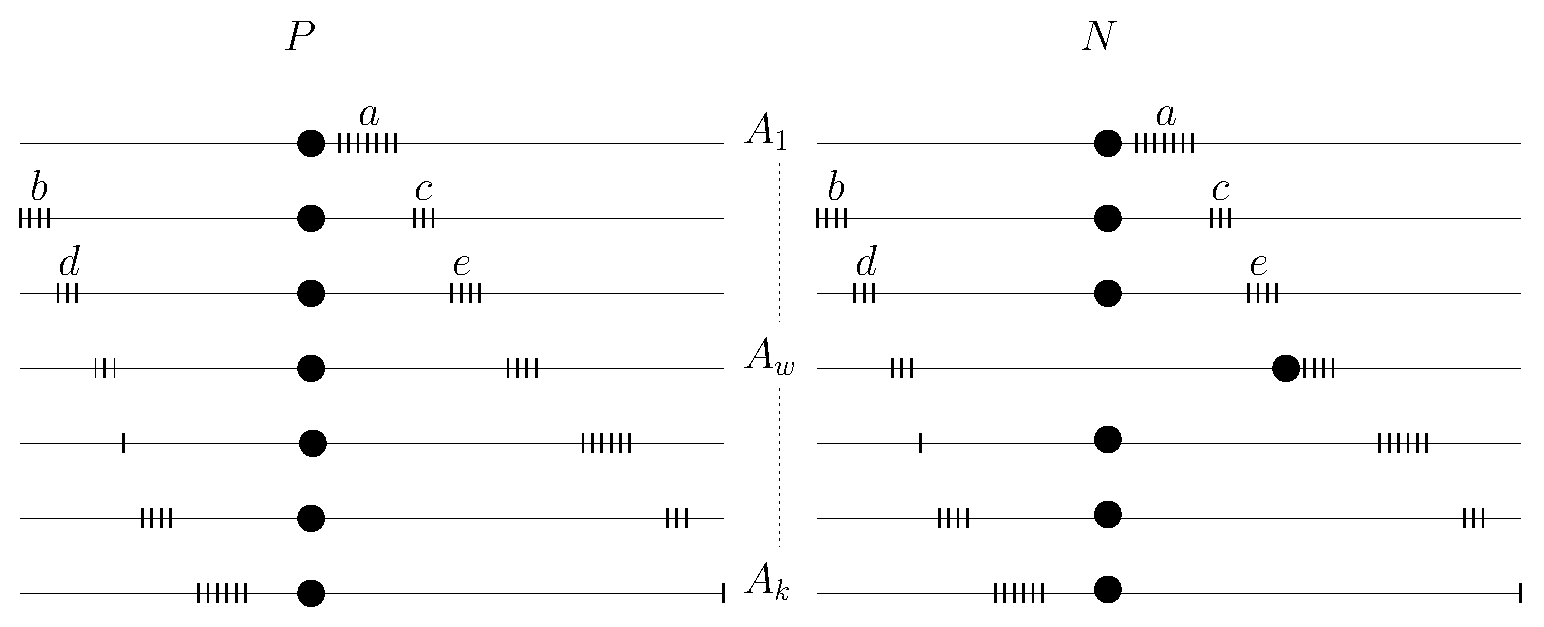
\includegraphics[angle=0,width=12cm]{PNdistribution}}
\caption{Distribution on $(P,N)$: each element of value $v$ is
represented by a dot of x-coordinate $v$, and large dots correspond to
the element at position $p_i$ in each array
$A_i$. \label{fig:PandNdistribution}}
\end{figure}

Let $x=A_1[1]$ be the first element of the first array.
%
Define $x$-comparisons to be the comparisons between any element and $x$.
%
Because of the special relative positions of the elements, a
comparison between two elements $b$ and $d$ in any arrays does not
yield more information than the two comparisons between $x$ and $b$
and between $x$ and $d$: the positions of elements $b$ and $d$
relative to $x$ permit to deduce their order.
%
Hence any algorithm performing $C$ comparisons between arbitrary
elements can be expressed as an algorithm performing no more than $2C$
$x$-comparisons, and any lower bound $L$ on the complexity of
algorithms using only $x$-comparisons is an $L/2$ lower bound on the
complexity of algorithms using comparisons between arbitrary elements.

The alternation of such instances is at most $4$, and the redundancy
of such instances is no more than $3+{1/(k{-}1)}$, which is less
than $4$:
%
\begin{itemize}
\item the interval $\left(-\infty,A_{1}[1]\right)$ is sufficient to
  certify that no element smaller than $x$ is in the intersection, and
  stands for a redundancy of at most $1$;
%
\item the interval $\left(A_{1}[n_1],+\infty,\right)$ is sufficient to
  certify that no element larger than $A_{1}[n_1]$ is in the
  intersection, and stands for a redundancy of at most $1$;
%
\item  the interval $\left[A_1[1],A_{1}[n_{1}]\right]$ is sufficient in $N$
to complete the partition-certificate, and stands for a redundancy of
at most $1$;
% 
\item  the singleton $\{x\}$ and the interval
$\left(A_1[1],A_{1}[n_{1}]\right]$ are sufficient in $P$ to complete
the partition-certificate, and stand for a redundancy of at most
$1{+}{1/(k-1)}$.
\end{itemize}

The only difference between instances $P$ and $N$ is the relative
position of the element $A_{w}[p_{w}]$ to the other elements composing
the instance, as described in Figure~\ref{fig:PandNdistribution}.
%
Any algorithm computing the intersection of $P$ has to find the
$(k-1)$ positions $\{p_2,\ldots,p_k\}$.
%
Any algorithm computing the intersection of $N$ has to find $w$ and
the
associated
position $p_w$.
%
Any algorithm distinguishing between $P$ and $N$ has to find $p_w$:
%
we will prove that it needs on average almost
${F/2}={(1/2)}\sum_{i=2}^k\log_2(2n_i+1)$ $x$-comparisons to do so on
a distribution corresponding to the uniform choice between an instance
$N$ and an instance $P$.

Consider a deterministic algorithm using
only $x$-comparisons to compute the intersection.
%
As the algorithm  has not distinguished between $P$ and $N$ till it
found $w$, let $X_i$ denote the number of $x$-comparisons performed
 in array $A_i$ for both $P$ or $N$.
%
Let $Y_i$ denote the number of $x$-comparisons performed  in
array $A_i$ for $N$;
%
and let $\xi_i$ be the indicator variable which equals $1$ exactly if
$p_i$ has been determined  on instance $P$.
%
The number of comparisons performed  is $C=\sum_{i=2}^k X_i$.
Restricting ourselves to arrays in which the position $p_i$ has been
determined, we can write $C\geq\sum_{i=2}^k X_i\xi_i
=\sum_{i=2}^k Y_i\xi_i$.

Let us consider $E(Y_i\xi_i)$: the expectancy can be decomposed as a
sum of probabilities $E(Y_i\xi_i){=}\sum_h\Pr\{Y_i\xi_i{\geq}h\}$, and
in particular
$E(Y_i\xi_i){\geq}\sum_{h=1}^{F_i}\Pr\{Y_i\xi_i{\geq}h\}$.
%
Those terms can be decomposed using the property
$\Pr\{a{\vee}b\}\leq\Pr\{a\}{+}\Pr\{b\}$:
%$\Pr\{Y_i\xi_i\geq h\}$
\begin{eqnarray}
\Pr \{ Y_i\xi_i\geq h \} 
&  =    & \Pr \{ Y_i\geq h \wedge \xi_i=1 \}   \nonumber\\
&  =    &  1 - \Pr \{ Y_i< h \vee \xi_i=0 \} \nonumber\\
&  \geq &  1 - \Pr \{ Y_i< h \} - \Pr \{ \xi_i=0 \} \nonumber\\
&  =    &  \Pr \{ \xi_i=1 \} -\Pr \{ Y_i< h \} \label{equation1}
\end{eqnarray}

The probability $\Pr\{Y_i<h\}$ is bounded by the usual decision
tree lower bound: if we consider the binary $x$-comparisons performed
 in set $A_i$, there are at most $2^{h}$ leaves at
depth less than $h$.
%
Since the insertion rank of $x$ in $A_i$ is uniformly chosen, these
leaves have the same probability and have total probability at most
$\Pr\{Y_i{<}h\}{\leq}{2^{h}/(2n_i+1)}{=}2^{h-F_i}$.
%
Those terms for $h\in\{1,\ldots,F_i\}$ form a geometric sequence whose
sum is equal to $2(1-2^{-F_i})$,
%
so $E(Y_i\xi_i) \geq F_i \Pr\{\xi_i=1\} - 2(1-2^{-F_i})$.
%
Then 
\begin{eqnarray}
E(C)\geq\sum_{i=2}^k E(Y_i \xi_i)
&\geq& \sum_{i=2}^k F_i \Pr\{\xi_i=1\}
      - \sum_{i=2}^k 2(1-2^{-F_i})
\nonumber\\ 
&\geq& \sum_{i=2}^k F_i \Pr\{\xi_i=1\}
      + 2\sum_{i=2}^k 2^{-F_i}  - 2(k-2).
\label{equation2}
\end{eqnarray}


Let us fix $p=(p_2, \ldots,p_k)$.
%
There are only $k-1$ possible choices for $w$.
%
The algorithm can only differentiate between $P$ and $N$ when it finds
$w$.
%
Let $\sigma$ denote the order in which these instances are dealt with
for $p$ fixed.
%
Then $\xi_i=1$ if and only if $\sigma_i\leq\sigma_w$, and so
 $\Pr\{\xi_i=1|p\}=\sum_{j:\sigma_j\geq\sigma_i}{F_j /  F}$.

Summing over $p$, and then over $i$, we get an expression of the first term in
Equation~(\ref{equation2}):
$$
\Pr\{ \xi_i=1 \} 
= \sum_{p} 
        \Pr \{ \xi_i=1 | p\} 
	\Pr \{ p\} 
= \sum_{p} 
	\sum_{j: \sigma_j \geq\sigma_i}
		{ F_j\over F} \Pr \{ p\} 
$$
$$
\sum_{i=2}^k F_i \Pr\{\xi_i =1\} 
=  \sum_{p} \sum_{i=2}^k \sum_{j : \sigma_j \geq \sigma_i }
	   { F_i F_j \over F}  \Pr \{ p\}
=  \sum_{p} \Pr \{ p\}
       \sum_{i=2}^k \sum_{j : \sigma_j \geq \sigma_i }
       \frac   {F_i F_j}
	       {F}.   		
$$
%
In the sum, each term ``$F_i F_j$'' appears exactly once,
and 
$$\left(\sum_i F_i\right)^2
=2\sum_i\sum_{i\leq j} F_i F_j - \sum_i {F_i}^2,$$ hence
 $$ \sum_{i=2}^k \sum_{j : \sigma_j \geq \sigma_i }  F_i F_j  
=\frac{1}{2} \left( 
\left( \sum_{i=2}^k F_i \right)^2 +  \sum_{i=2}^k {F_i}^2 
\right),$$
which is independent of $p$.
%
Then we can conclude:
$$
\sum_{i=2}^k F_i \Pr \{\xi_i=1\} 
= \frac{1}{2} \frac{1}{F}
     \left( \left(\sum_{i=2}^k F_i\right)^2 + \sum_{i=2}^k {F_i}^2 \right) 
     \sum_{p}\Pr\{p\}\\
%&\geq& \frac{1}{2} \frac{1}{F} \left(\sum_{i=2}^k F_i\right)^2\\
= \frac{1}{2} \sum_{i=2}^k F_i .
$$ 
%
Plugging this into Equation~(\ref{equation2}), we obtain a lower bound
on the average number of $x$-comparisons $E(C)$ performed by any
deterministic algorithm which performs only $x$-comparisons, of
$(1/2)\sum_{i=2}^k F_i+2\sum_{i=2}^k 2^{-F_i}-2(k{-}2)$, which
is equal to $(1/2)\sum_{i=2}^k\log_2(2n_i{+}1) + 2\sum_{i=2}^k {1/(2n_i{+}1)} - 2(k{-}2)$.
%
This  implies a lower bound of 
${(1/4)}\sum_{i=2}^k\log_2(2n_i{+}1) + \sum_{i=2}^k {1/(2n_i{+}1)} - (k{-}2)$ 
%
on the average number of comparisons performed by
{\em any} deterministic algorithm, hence the result.
\qed\end{proof}

%
\begin{lemma}\label{lem:generaldistribution}
For any $k\geq 2$, $0{<}n_1{\leq}\ldots{\leq}n_k$ and
$\rho{\in}\{4,\ldots,4n_1\}$, there is a distribution on instances of
the intersection problem of signature at most $(k,n_1,\ldots,n_k)$, of
alternation and redundancy at most $\rho$, such that any deterministic
algorithm performs on average $\Omega(\rho \sum_{i=1}^k \log(n_i/\rho))$ comparisons.
\end{lemma}
\begin{proof}
Let's draw $p{=}\lfloor\rho/4\rfloor$ pairs
$(P_j,N_j)_{j\in\{1,\ldots,p\}}$ of sub-instances of signature
$(k,\lfloor n_1/p\rfloor,\ldots,$ $\lfloor n_k/p\rfloor)$ from
the distribution of Lemma~\ref{lem:elementproblem}.
%
As $\rho\leq4n_1$, $p\leq n_1$ and $\lfloor n_1/p\rfloor>0$, the sizes
of all the arrays are positive.
%
Let's choose uniformly at random each sub-instance $I_j$ between the
sub-instance $P_j$ which intersection is a singleton and the
sub-instance $N_j$ which intersection is empty, and form a
larger instance $I$ by unifying the arrays of same index from each
sub-instance, such that the elements from two different sub-instances
never interleave, as in Figure~\ref{fig:generaldistribution}.
\begin{figure}
\centerline{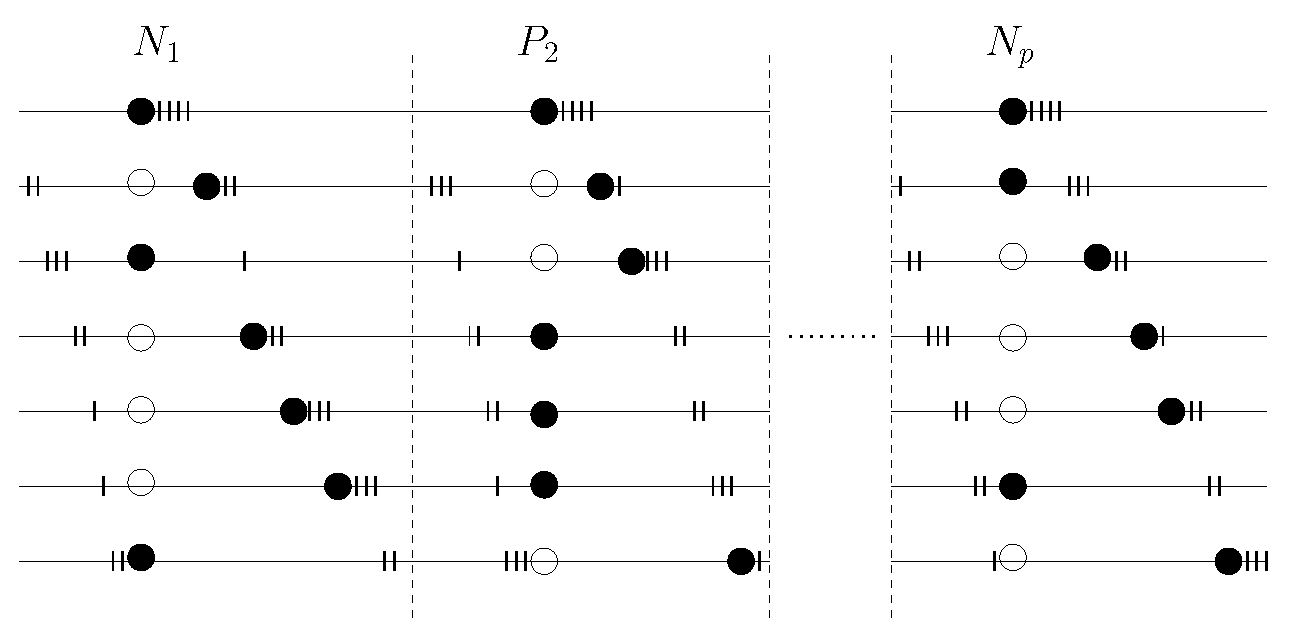
\includegraphics[angle=0,width=8cm]{generaldistribution.eps}}
\caption{$p$ elementary instances unified to form a single large instance.}\label{fig:generaldistribution}
\end{figure}

This defines a distribution on instances of alternation and redundancy
at most $\rho$ (as $4p=4\lfloor\rho/4\rfloor\leq\rho$), and of
signature at most $(k,n_1,\ldots,n_k)$.
%
Solving this instance implies to solve all the $p$ sub-instances.
Lemma~\ref{lem:elementproblem} gives a lower bound of
$(1/4)\sum_{i=2}^k\log (2n_i/p+1)+\sum_{i=2}^k{1/(2n_i{+}1)}-k{+}2$
comparisons on average for each of the $p$ sub problems, hence a lower
bound of
%
$$(p/4)
  \sum_{i=2}^k   \log(2n_i/p+1)  
               +p\left( \sum_{i=2}^k { 1 / (2n_i/p{+}1) }
                                 -k{+}2
                 \right)
,$$
%
which is $\Omega(\rho\sum_{i=1}^k\log (n_i/\rho))$.  \qed\end{proof}
%


\subsubsection{Application to Alternation}
\label{sec:appl-altern}


Indeed, among instances of same signature and alternation, it is
possible to prove a tight bound on the randomized complexity of the
intersection problem: by providing a difficult distribution of
instances and using the minimax principle, we prove a lower bound on
the complexity of any randomized algorithm solving the
problem~\cite{adaptiveIntersectionAndTThresholdProblems}.
%
\begin{theorem}[Alternation Lower Bound~\cite{adaptiveIntersectionAndTThresholdProblems}]\label{th:alternationLB}
For any $k{\geq} 2$, $0{<}n_1{\leq}\ldots{\leq}n_k$ and
$\delta{\in}\{4,\ldots,4n_1\}$,
%
and for any randomized algorithm $A_R$ for the intersection problem,
%
there is an instance of signature at most $(k,n_1,\ldots,n_k)$ and
alternation at most $\delta$,
%
such that $A_R$ performs $\Omega(\delta\sum_{i=1}^k\log(n_i/\delta))$
comparisons on average on it.
\end{theorem}
\begin{proof}
This is a simple application of Lemma~\ref{lem:generaldistribution}
(stated and proved in Section~\ref{sec:lowerbound})
and of the Yao-von Neumann principle \cite{vonneumann1944,sion58,yao}:
\begin{itemize}
\item Lemma~\ref{lem:generaldistribution} gives a distribution for
$\delta\in\{4,\ldots,4n_1\}$ on instances of
alternation {\em at most} $\delta$,
\item Then the Yao-von Neumann principle permits to deduce from this
distribution a lower bound on the worst case complexity of randomized
algorithms.  \qed\end{itemize}
\end{proof}

On the other hand, the simple deterministic algorithm of
Section~\ref{sec:alternation} reaches this lower bound.
%
As the class of deterministic algorithms is contained in the class of
randomized algorithms, this proves that the bound for the alternation
analysis is tight for randomized algorithms.
%



\subsubsection{Application to Redundancy}
\label{sec:appl-redund}





\begin{theorem}[Redundancy Lower Bound~\cite{optimalityOfRandomizedAlgorithmsForTheIntersectionProblem}]\label{th:standalonelowerbound} \label{th:redundancyLB}
For any $k\geq 2$, $0{<}n_1{\leq}\ldots{\leq}n_k$ and
$\rho\in\{4,\ldots,4n_1\}$, 
%
and for any randomized algorithm $A_R$ for the intersection problem,
%
there is an instance of signature at most $(k,n_1,\ldots,n_k)$, and
redundancy at most $\rho$,
%
such that $A_R$ performs $\Omega(\rho\sum_{i=1}^k\log(n_i/\rho))$
comparisons on average on it.
\end{theorem}

\begin{proof}
The proof is identical to the proof of Theorem~\ref{th:alternationLB},
as the instances generated by the proof are of alternation equal to
their redundancy.
%
This is a simple application of Lemma~\ref{lem:generaldistribution} and
of the Yao-von Neumann principle \cite{vonneumann1944,sion58,yao}:
\begin{itemize}
\item Lemma~\ref{lem:generaldistribution} gives a distribution for
$\rho\in\{4,\ldots,4n_1\}$ on instances of redundancy {\em at most}
$\rho$, 
\item Then the Yao-von Neumann principle permits to deduce from this
distribution a lower bound on the worst case complexity of randomized
algorithms.  \qed\end{itemize}
\end{proof}


This analysis is more precise than the lower bound previously
presented~\cite{adaptiveIntersectionAndTThresholdProblems}, where the
additive term in $-k$ was ignored, although it makes the lower bound
trivially negative for large values of the difficulty $\delta$.
%
Here the additive term is suppressed for $\min_i n_i\geq128$, and the
multiplicative factor between the lower bound and the upper bound is
reduced to $16$ instead of $64$.
%
This technique can be applied to the alternation analysis of the
intersection with the same result.
%
Note also that a multiplicative factor of $2$ in the gap comes from
the unbounded searches in the algorithm, and can be reduced using a
more complicated algorithm for the unbounded
search~\cite{anAlmostOptimalAlgorithmForUnboundedSearching}.



One could wonder how the lower bound evolves for redundancy values
larger than $4n_1$.
%
The following result shows that no instance with such redundancy can
exist.
%
\begin{lemma}\label{lem:rhoupperbound}
For any $k\geq 2$ and
$0{<}n_1{\leq}\ldots{\leq}n_k$, any instance of signature
$(k,n_1,\ldots,n_k)$ has redundancy $\rho$ at most $2n_1{+}1$.
\end{lemma}
\begin{proof}
First observe that there is always a partition-certificate of size
$2n_1+1$. Then that the redundancy of any partition-certificate is by
definition smaller than the size of the partition. Hence the result.
\qed\end{proof} 
%
Note that this does not contradict the result from
Lemma~\ref{lem:generaldistribution}, which defines a distribution of
instances of redundancy {\em at most} $4n_1$.

\subsection{Comparisons between the analysis}\label{sec:comparison}

The redundancy analysis is strictly finer than the alternation analysis:
%
some algorithms, optimal for the alternation analysis, are not optimal
anymore in the redundancy analysis (Theorem~\ref{th:finer}),
%
and any algorithm optimal in the redundancy analysis is optimal in the
alternation analysis (Theorem~\ref{th:strictlyfiner}).
%
So the {\tt Rand Intersection} algorithm is theoretically better than
its deterministic variant in the comparison model, and the redundancy
analysis permits a better analysis than the alternation analysis.

%
\begin{theorem}\label{th:finer}
For any $k\geq 2$, $0{<}n_1{\leq}\ldots{\leq}n_k$ and
$\rho\in\{4,\ldots,4n_1\}$, 
%
and for any deterministic algorithm for the intersection problem,
%
there is an instance of signature at most $(k,n_1,\ldots,n_k)$, and
redundancy at most $\rho$,
%
such that this algorithm performs $\Omega(k\rho\sum_i\log(n_i/k\rho))$
comparisons on it.
\end{theorem}
\begin{proof}
The proof uses the same decomposition than the proof of
Theorem~\ref{th:standalonelowerbound}, but uses an adversary argument
to obtain a deterministic lower bound.
%
Build $\delta={k\rho/3}$ sub-instances of signature
$(k,\lfloor{n_1/\delta}\rfloor,\ldots,\lfloor{n_k/\delta}\rfloor)$,
redundancy at most $3$, such that $x=A_1[1]$ is present in
roughly half of the other arrays, as in
Figure~\ref{fig:halffullsubinstance}.



On each sub-instance an adversary can force any deterministic algorithm
to perform a search in each of the arrays containing $x$, and in a
single array which does not contain $x$.
%
Then the deterministic algorithm performs
$(1/2)\sum_{i=2}^k\log{(n_i/\delta)}$ comparisons for each
sub-instance.
%
\begin{figure}
\hfill
\begin{minipage}{0.33\textwidth}
\centerline{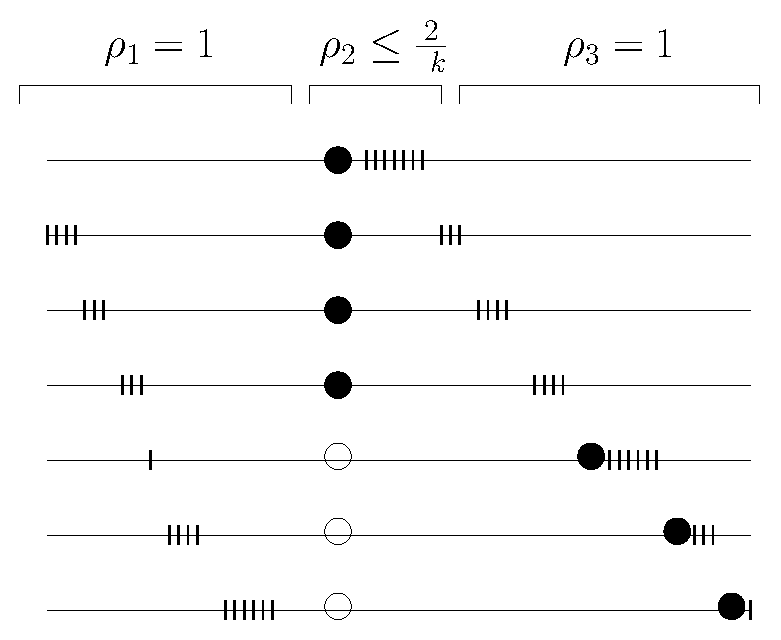
\includegraphics[angle=0,height=3.3cm]{halffullsubinstance.eps}}
\caption{Element $x$ is present in half of the arrays of the sub-instance.\label{fig:halffullsubinstance}
}
\end{minipage}
\hfill
\begin{minipage}{0.66\textwidth}
\centerline{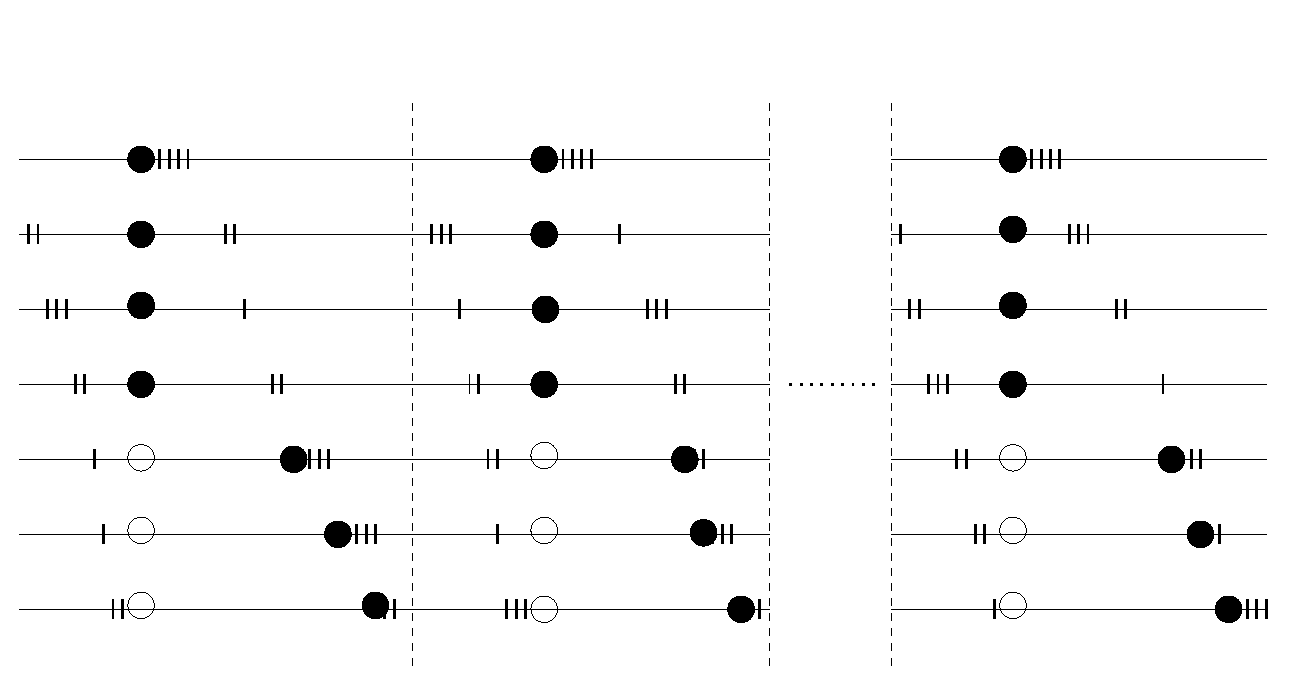
\includegraphics[angle=0,height=3.5cm]{halffullinstance.eps}}
\caption{The adversary performs several strategies in parallel, one
for each
sub-instance. \label{fig:halffullinstance}}\end{minipage}\hfill \hfill
\hfill \hfill
\end{figure}
%
In total over all sub-instances, the adversary can force any
deterministic algorithm to perform
${(\delta/2)}\sum_{i=2}^k\log{(n_i/\delta)}$ comparisons, i.e.
${(k\rho/4)}\sum_{i=2}^k\log{(n_i/k\rho)}$, which is
$\Omega({k\rho}\sum_{i=2}^k\log{(n_i/k\rho)})$.
\qed\end{proof}
%
As $x\log(n/x)$ is a function increasing with $x$,
$k\rho\sum_i\log(n_i/k\rho)$ is several times larger than the lower
bound $\rho\sum_i\log(n_i/\rho)$, hence no deterministic algorithm can
be optimal in the redundancy analysis.
%
\begin{theorem}\label{th:strictlyfiner}
Any algorithm optimal in the redundancy analysis is optimal in the
alternation analysis.
\end{theorem}
\begin{proof}
By definition of the redundancy $\rho$ and of the alternation $\delta$
of an instance, $\rho\leq\delta$.
%
So if an algorithm performs $O(\rho\sum \log{n_i/\rho})$
comparisons, it also performs $O(\delta\sum\log{n_i/\delta})$
comparisons.
%
Hence the result, as this is the lower bound in the alternation analysis.
\qed\end{proof}


This proves also that the measure of difficulty of
Demaine~\etal~\cite{dlm} is not comparable with the measure of
redundancy, as it is not comparable with the measure of
alternation~\cite[Section~2.3]{deterministicAlgorithmForTheTThresholdSetProblem}.
%
This means that the two measures are complementary, without being
redundant in any way, as it was for the alternation.
%
All those measures describe the difficulty of the instance:
\begin{itemize}
\item the {\em alternation}~\cite[Section~2.3]{deterministicAlgorithmForTheTThresholdSetProblem}
describes the number of key blocks of consecutive elements in the
instance;
\item the {\em gap cost}~\cite{dlm} describes the repartition of the
size of those blocks;
\item the {\em
redundancy}~\cite{optimalityOfRandomizedAlgorithmsForTheIntersectionProblem}
describes the difficulty to find each
block.
\end{itemize}
%
But only the {\em gap cost} and the {\em redundancy} matter, because the
alternation analysis is reduced to the redundancy analysis.



\section{Weighted $t$-Threshold Set}
\label{sec:t-threshold-set}



Conjunctive queries are well known. Indeed, most search engines
implement them.
% 
Given a list of labels (e.g.  keywords), the answer consists of all
the objects (e.g. webpage references) which are associated with all of
the labels.
%
Given an index such as described in the section above, solving a
conjunctive query composed of $\nbkeywords$ labels implies computing
the intersection of $\nbkeywords$ rows in a binary relation, which is
a well studied
problem~\cite{aFastSetIntersectionAlgorithmForSortedSequences,experimentalAnalysisOfAFastIntersectionAlgorithmForSortedSequences,dlm,dlmAlenex}


As an empty intersection can be an uninformative answer to a
conjunctive query, we should consider other approaches. 
%
Researchers in information retrieval suggest a number of ways to deal
with this problem.
%
For example, one can relax both queries and document index in a number
of different ways that are summarized by Bordogna and
Pasi~\cite{DBLP:conf/essir/BordognaP00}.
%
Barbay and Kenyon~\cite{adaptiveIntersectionAndTThresholdProblems}
proposed the adaptive algorithm to answer the query where for a given
parameter $\threshold$ the answer consists of the references matching
at least $\threshold$ of the $\nbkeywords$ labels composing the query.
%
Given an index such as described in the section above, solving this
new type of query implies computing the {\em threshold set} of 
$\nbkeywords$ rows in a binary relation, the set of objects associated
with at least $\threshold$ labels among the $\nbkeywords$ specified.

Barbay and Veraskouski
\cite{adaptiveAlgorithmsForWeightedQueriesOnWeightedBinaryRelationsAndLabeledTrees}
extended further this type of query to {\em weighted threshold}
queries, by considering
%
weighted queries $\Q:[\nblabels]\rightarrow\{0,\ldots,\maxWeightQ\}$,
where $\nblabels$ is the number of admissible keywords, and
%
weighted binary relations 
$\R:[\nblabels]\times[\nbobjects]\rightarrow\{0,\ldots,\maxWeightR\}$
~\footnote{By $[m]$ we denote $\{1, \ldots, m\}$ for any integer number $m$.}.
%
The {\em score} of an object $\objectx$ relative to a query $\Q$ on a
relation $\R$ is then defined as the linear combination of those
weights, i.e. $\score(\R,\Q,\objectx) = \sum_{\labelx \in
  [\nblabels]}{\Q(\labelx)\R(\labelx,\objectx)}$, that corresponds to
the notion of the {\em Retrieval Status Value} (or RSV) described by
Bordogna and Pasi~\cite{DBLP:conf/essir/BordognaP00}.
%
The answer to a query with parameter $\threshold$ is the set of
objects with score at least~$\threshold$: this definition matches the
original one from Barbay and Kenyon when each weight is either null or
unitary (the {\em unweighted} case).

We define the {\em alternation} of a weighted threshold set instance
as the size $\difficulty$ of the smallest possible
partition-certificate of the instance.
%
\begin{LONG}
  The alternation is related to the {\em non-deterministic} complexity
  of the instance, as it corresponds to the complexity of a
  non-deterministic algorithm which would produce the shortest
  partition-certificate of the instance.
\end{LONG}
% 
In the unweighted case (where all weights are unitary), if no object
match the query then the alternation is exactly the non-deterministic
complexity of the instance, i.e. the complexity of the best
non-deterministic algorithm checking the answer to the query.

\begin{figure}
  \centering
$$  \begin{array}[b]{cc|c|c|c|c|c|c|cccc|ccccc|cccccc|cccccccc}

    & 
    \multicolumn{7}{}  											                         &                    & & &
 1  &  2 &  3 &  4 &  5 &  6 &  7 & 8  &  9 &  10 &  11 & 12 &  13 &  14 & 15 & 16  & 17 & 18  &      &    
\\ \cline{3-8} \cline{11-28}


    \mbox{Music} & \rightarrow      
& 1                                & 8       & 10      & 12           & 15      & 17                 & & \rightarrow &
  1  &  . &  . &  . &  . &  . &  . & 1  &  . &  1 &  . &  1 &  . &  . &  1 &  . &  1 &  .  &   &    
\\ \cline{3-8}
    \mbox{Jazz} & \rightarrow
    & 2       & 4       & 6            & 9       & 11      & 13                                      & & \rightarrow &
  . & 1  &  . & 1  &  . & 1  &  . &  . & 1  &  . &  1 &  . &  1 &  . &  . &  . &  . &  . &     &    
\\ \cline{3-8}
    \mbox{Rock} & \rightarrow      
         & 3       & 5       & 7                                & 14      & 16      & 18             & & \rightarrow &
  . &  . & 1  &  . & 1  & .  & 1  &  . &  . &  . &  . &  . &  . &  1 &  . &  1 &  . &  1 &    
\\ \cline{3-8}
  \end{array}$$
  \begin{minipage}{.9\linewidth}
    \caption{ An example of how a conjunctive query composed 
      of three keywords corresponds to the
      intersection of the three corresponding sets.  
      % 
      The alternation of the instance is $\difficulty=4$, 
      the number of intervals of a partition certificate 
      where each interval has an empty intersection with at least one of the sets.
      % 
      Barbay and Kenyon's algorithm performs
      $7{\leq}\difficulty\nbkeywords{=}12$ searches (for the numbers
      $1,2,3,8,9,14,15$).  \label{fig:sequentialExample} }
  \end{minipage}
\end{figure}

Barbay and Kenyon~\cite{adaptiveIntersectionAndTThresholdProblems}
proved that any randomized algorithm performs
$\Omega(\difficulty\nbkeywords)$ searches in the worst case over
instances of difficulty $\difficulty$ on $\nbkeywords$ labels, and
proposed an optimal deterministic algorithm for the unweighted case on
sorted arrays.
%
We analyze the complexity of the algorithms in terms of search and
priority queue operations, where a priority queue operation is either an insertion or a
deletion from a priority queue, and where each search operation is a search for
the particular object in a data structure representing an ordered list
of objects.
%
We propose an optimal algorithm for the weighted case with any data
structure supporting the search for the insertion rank in an indexed
set:

\begin{theorem}\label{th:threshold-set}
  Consider a weighted binary relation
  $\R:[\nblabels]\times[\nbobjects]\rightarrow\{0,\ldots,\maxWeightR\}$,
  a weighted query
  $\Q:[\nblabels]\rightarrow\{0,\ldots,\maxWeightQ\}$, and a
  non-negative integer $\threshold$.
  % 
  There is an algorithm that computes the threshold set for $\Q$ on
  $\R$ with threshold-value of $\threshold$ in $\bigo(\difficulty\nbkeywords)$
  search and priority queue operations, where
  % 
  $\difficulty$ is the alternation of the instance and
  % 
  $\nbkeywords$ is the number of labels of positive weight in~$\Q$.
\end{theorem}

  \begin{algorithm}
    \centering
    \caption{Algorithm  answering Threshold Set queries }
    \label{alg:ThresholdOnBinRel}
    \begin{algorithmic}
      \STATE Set $\objectx$ to $-\infty$, 
      $\setNO$ and $\setYES$ to $\emptyset$
      and $\setMAYBE$ to the set of all labels of non-null weight;

      \STATE \idtt{Update}$(\objectx,\setYES,\setNO,\setMAYBE,\scoremin,\scoremax)$ 
      using Algorithm~\ref{alg:choiceBR};

      \WHILE{$\objectx<\infty$}

        \STATE Set $\labelx$ to the next label from $\setMAYBE$ in round
        robin order, and deduct $\maxWeightR\Q(\labelx)$ from
        $\scoremax$;

        \STATE Search for the insertion rank of $\objectx$ among the
        objects labeled $\labelx$;

        \IF{$\objectx$ is associated with a label $\labelx$}
          \STATE Move $\labelx$ from $\setMAYBE$ to $\setYES$;
          \STATE Add $\Q(\labelx)\R(\labelx,\objectx)$ to
          $\scoremin$ and $\scoremax$;
          \STATE {\bf if} {$\threshold\leq\scoremin$} 
                 {\bf then } Output $\objectx$;
        \ELSE    
          \STATE Move $\labelx$ from $\setMAYBE$ to $\setNO$;
        \ENDIF

        \IF{$\threshold \le \scoremin$ or $\threshold>\scoremax$}
           \STATE \idtt{Update}$(\objectx,\setYES,\setNO,\setMAYBE,\scoremin,\scoremax)$;
        \ENDIF

      \ENDWHILE
    \end{algorithmic}
  \end{algorithm}

  \begin{PROOF}
    \begin{proof}[of Theorem~\ref{th:threshold-set}]
      Consider the steps of Algorithm~\ref{alg:ThresholdOnBinRel}:
      given a query $\Q$ with $\nbkeywords$ positive weights and a
      threshold-value $\threshold$, the algorithm computes the set of
      objects scoring at least $\threshold$ for a weighted binary
      relation $\R$ associating objects with labels.

      Our algorithm goes through a number of phases. At each phase it
      considers one object $\objectx$, in increasing order, and bounds
      its score by an interval $[\scoremin,\scoremax]$.
  %
      The algorithm can decide whether $\objectx$ belongs to the
      result set through this interval and without computing the
      object's exact score
      ($\threshold\leq\scoremin\leq\score(\objectx)$).
  % 
      On the other hand, if for a given interval of consecutive
      objects there is a set of labels not associated with any of them
      with large total weight, this interval certifies that none of
      those objects belongs to the result set
      ($\score(\objectx)\leq\scoremax<\threshold$).
  % 
      The key issue of the algorithm is the choice of the values of
      $\objectx$ and of the labels to consider.

      This choice is described in Algorithm~\ref{alg:choiceBR}, which
      is based on the decomposition of the set of labels of positive
      weights in three disjoint sets: $\setYES$, $\setMAYBE$ and
      $\setNO$:
  %
      \begin{itemize}
      \item $\setYES$ corresponds to the labels already known to be
        associated with the current value of $\objectx$. It can be
        implemented as a simple set, for instance in an array.
      \item $\setMAYBE$ corresponds to the labels which could be
        associated with the current value of $\objectx$. It is
        implemented as a FIFO queue so that each label in it is
        considered equally often.
      \item $\setNO$ corresponds to the labels which are known not to
        be associated with the current value of $\objectx$. It is
        implemented as a priority queue of at most $\nbkeywords$
        elements, and the labels $\labelx$ it contains are ordered by
        the value of the first object larger than $\objectx$
        associated with label $\labelx$.
      \end{itemize}
  % 
      The values of the bounds $\scoremin$ and $\scoremax$ on the
      potential score of $\objectx$ are direct consequences of those
      definitions: $\scoremin$ depends on the weights of the labels in
      $\setYES$, i.e.
      $\scoremin=\sum_{\labelx\in\setYES}\Q(\labelx)\R(\labelx,\objectx)$;
      and $\scoremax$ adds the maximum potential weights of the labels
      in $\setMAYBE$ to $\scoremin$, i.e.
      $\scoremax=\scoremin+\sum_{\labelx\in\setMAYBE}\Q(\labelx)\maxWeightR$.

      To choose a new value for $\objectx$, the algorithm removes
      labels from the set $\setMAYBE$ till it reaches a critical
      weight, where removing any other label would make it impossible
      for an object matching only the labels of $\setMAYBE$ to score
      above the threshold.
  % 
      Then, the smallest object potentially in the result set
      corresponds to the first label of the priority queue
      implementing set $\setNO$.
 

      %%%%%%%%%%%%%%%%%% ADAPTIVE
      %%%%%%%%%%%%%%%%%% ANALYSIS %%%%%%%%%%%%%%%%%%%%%%%%%%%%%%%%%%%%%%%%%

      Consider a phase of the execution where the algorithm is
      processing an interval of the partition-certificate consisting
      of only one object $\objectx$.
      Algorithm~\ref{alg:ThresholdOnBinRel} performs at most
      $\nbkeywords$ iterations of the main loop to decide whether
      $\objectx$ has enough score or not without updating $\objectx$
      (through Algorithm~\ref{alg:choiceBR}). Once the decision about
      $\objectx$ is made, the algorithm updates $\objectx$ and moves
      to the next phase. Updating of $\objectx$ takes not more than
      $\nbkeywords$ loop iterations of Algorithm~\ref{alg:choiceBR}.
      Thus during each phase, the algorithm performs at most
      $\bigo(\nbkeywords)$ search and priority queue operations.

      Consider a phase corresponding to the interval of the
      partition-certificate that does not have any objects with enough
      score and a subset $S$ of labels that are not associated with
      any of the objects in this interval.
      Algorithm~\ref{alg:ThresholdOnBinRel} may update $\objectx$ more
      than once during the same phase. We prove the upper bound on the
      number of operations through considering the way the algorithm
      moves labels from one set to another.
  
      The only way Algorithm~\ref{alg:ThresholdOnBinRel} moves labels
      is from set $\setMAYBE$ to either set $\setYES$ or set $\setNO$.
      Algorithm~\ref{alg:choiceBR}, on the other hand, move labels
      from $\setYES$ to $\setMAYBE$, from $\setMAYBE$ to $\setNO$, and
      from $\setNO$ to $\setYES$ in this order. As it cannot move
      labels that are in $S$ to $\setYES$, the algorithm has the only
      possible loop $\setMAYBE \longrightarrow \setNO \longrightarrow
      \setYES \longrightarrow \setMAYBE$ for these labels.
  
      However, the algorithm does not move any labels from $S$ that it
      already moved to $\setNO$ during the processing of the same
      interval, because the label's successor is out of the current
      interval and cannot be processed in the current phase. While the
      algorithm retrieves labels from set $\setMAYBE$ in round-robin
      order, it cannot retrieve any label from set $\setMAYBE$ for the
      second time until all the labels from subset $S$ appear in set
      $\setNO$, which effectively means that the next element
      $\objectx$ will be outside of the interval and the algorithm
      proceeds to the new phase. While it takes a constant time for
      the algorithm to move each label from set $\setMAYBE$ back to
      set $\setMAYBE$, it needs $\bigo(\nbkeywords)$ search and
      priority queue operations to complete this phase.
  
      As the algorithm spends $\bigo(\nbkeywords)$ to complete any
      phase, and any instance has $\difficulty$ intervals that
      correspond to $\difficulty$ phases, the total complexity of the
      algorithm is $\bigo(\difficulty \nbkeywords)$.  \qed
    \end{proof}
  \end{PROOF}
      \begin{algorithm}
        \begin{algorithmic}
          \caption{\idtt{Update}$(\objectx,\setYES,\setNO,\setMAYBE,\scoremin,\scoremax)$}
          \label{alg:choiceBR}
 
          \STATE Add all the labels from $\setYES$ to the set
          $\setMAYBE$ and set $\scoremax$ to
          $\sum_{\labelx\in\setMAYBE}\Q(\labelx)\maxWeightR$; \STATE
          Choose a label $\labelx$ in round-robin order from
          $\setMAYBE$;

          \WHILE{$\scoremax-\Q(\labelx)\maxWeightR \ge \threshold$}
          \STATE Deduct $\Q(\labelx)\maxWeightR$ from $\scoremax$, and
          move $\labelx$ from $\setMAYBE$ to $\setNO$; \STATE Choose a
          label $\labelx$ in round-robin order from $\setMAYBE$;
          \ENDWHILE

          \STATE Find the subset $S\subset\setNO$ of labels $\labelx$
          such that the successor of $\objectx$ among the objects
          labeled $\labelx$ is minimal;

          \STATE Move all the labels of $S$ from $\setNO$ to
          $\setYES$, and set $\scoremin$ to
          $\sum_{\labelx\in\setYES}\Q(\labelx)\R(\labelx,\objectx)$;
      
          \STATE Update $\objectx$ to its successor among the objects
          labeled $\labelx$, for any label in $\setYES$;
        \end{algorithmic}
      \end{algorithm}

  Note that $\nbkeywords$ is the number of labels with a positive weight.
  % 
  If the binary relation is implemented by postings lists, and the
  priority queue is implemented using a heap, the complexity of the
  algorithm is $\bigo ( \difficulty \nbkeywords \lg (n / (\difficulty
  \nbkeywords)) + \difficulty \nbkeywords \lg {\nbkeywords } )$, where
  $n$ is the sum of the sizes of all postings lists and $\nbkeywords$
  is the maximum size of the priority queue.
  % 
  If the binary relation is implemented using
  Barbay~\etal's~\cite{weightedQueriesOnBinaryRelationsAndMultiLabeledTrees}
  succinct encoding and the priority queue is implemented using
  Andersson and
  Thorup's~\cite{tighterWorstCaseBoundsOnDynamicSearchingAndPriorityQueues}
  structure, the complexity of the algorithm is
  $\bigo(\difficulty\nbkeywords\lg\lg\nblabels +
  \difficulty\nbkeywords(\lg\lg\nbkeywords)^2)$ in the RAM model with
  word size $\Theta(\lg\max\{\nblabels,\nbobjects\})$.













\section{Perspectives}
\label{sec:perspectives}


The $t$-threshold set and opt-threshold set
problems~\cite{deterministicAlgorithmForTheTThresholdSetProblem} are
natural generalizations of the intersection problem, which could be
useful in indexed search engines.
%
The redundancy seems to be important in the complexity of these
problems as well, but a proper measure is harder to define in this
context.
%
As similar techniques are applied to solve queries on semi-structured
documents~\cite{indexTreesForDescendantTreeQueriesInTheComparisonModel},
the redundancy could be useful in this domain too, but the definition
of the proper measure of difficulty is even more evasive in this
context.
%
More generally, the set operations are combined in practice in a
recursive way, forming Union/Intersection trees.
%
Farzan~\etal~\cite{worstCaseOptimalUnionIntersectionExpressionEvaluation}
studied the non-adaptive complexity of the evaluation of such
expressions: the adaptive analysis of such a problem is still an open
problem.


Demaine~\etal~\cite{dlmAlenex} performed experimental measurements of
the performance of various deterministic algorithms for the
intersection on their own data using some queries provided by
\texttt{Google}.
%
We performed similar measurements for the deterministic and randomized
version of our algorithm, using the same queries and a larger set of
data, also provided by Google.
%
The results are quite disappointing, as the randomized version of the
algorithm does not perform better than the deterministic one in term
of the number of comparisons or searches, and much worst in term
of runtime.
%
The fact that the number of comparisons and the number of
searches are roughly the same indicates that most instances of
this data set either have a redundancy close to the alternation,
because the elements searched are in many of the arrays, or are so
easy that both algorithms perform equally well on it.
%
The fact that the runtime is worse is probably linked to the
performance of prediction heuristics in the hardware: a deterministic
algorithm is easier to predict than a randomized one.
%
It would be interesting to see if those negative results still holds
for queries with more keywords and on some data sets such as those
from relational databases, which can exhibit more correlation between
keywords.



While we restricted our definition of the intersection problem to set
of arrays and analyzed it in the comparison model, it makes sense to
consider other structures for sorted sets, especially in the context
of cached or swapped memory, or succinct encodings of
dictionaries.
%
The {\em hierarchical memory}~\cite{cacheObliviousAlgorithms} seems
promising for this kind of application, and
Bender~\etal~\cite{exponentialStructuresForEfficientCacheObliviousAlgorithms}
proposed a data structure and a {\em cache oblivious} algorithm to
perform unbounded searches (implemented as finger searches).
%
Our algorithm can easily be adapted to this model, to perform
$O(\rho\sum(\log_B(n_i/\rho)+\log^*(n_i/\rho)))$ I/O transfers at the
level of cache size~$B$.


\def\select{\hbox{\tt select}}
\def\rank{\hbox{\tt rank}}
%
In most of the intersection algorithms, the interactions with each set
are limited to accessing an element given its rank ($\select$ operator)
and searching for the insertion rank of an element in it ($\rank$
operator): those algorithms can be used with any set implementation
which provides those operators.
%
For instance, using sorted arrays such as in this paper, the $\select$
operator takes constant time while the $\rank$ operator takes
logarithmic time in the size of the set.
%
While the results of this paper are optimal in the comparison model,
it is not necessary optimal in more general models: the computational
complexity of the search operators is a trade-off with the size of the
encoding of the set.
%
For instance, consider a set of $n$ elements from a universe of size
$m$:
Raman~\etal~\cite{succinctIndexableDictionariesWithApplicationsToEncodingKAryTreesAndMultisets}
propose a succinct encoding of Fully Indexable Dictionaries using
$\log {m \choose n} + o(m)$ bits to provide $\select$ and $\rank$
operators in constant time.
%
On the other side of the time/space trade-off, Beame and
Fish~\cite{optimalBoundsForThePredecessorProblem} proposed a more
compact encoding, using $O(n)$ words of $\log m$ bits to provide
$\select$ and $\rank$ operators in time $O(\sqrt{ \log n / \log \log
  n})$.
%
Encoding the sets using any of those schema would tremendously improve
the computational complexity of the intersection, at a small cost in
space, which could result in much faster search engines.




%%% Local Variables: 
%%% mode: latex
%%% TeX-master: "adaptiveAnalysisOfAlgorithm"
%%% End: 
 
%%
%% adaptivePatternMatching.tex
%% 
%% Made by Jeremy Barbay
%% Login   <jbarbay@condorito>
%% 
%% Started on  Thu Apr 17 18:30:35 2008 Jeremy Barbay
%% Last update Thu Apr 17 18:30:35 2008 Jeremy Barbay
%%

\chapter{Pattern Matching in Trees}
\label{cha:pattern-matching}


\begin{definition}
  A {\bf multi-labeled tree} is an ordinal tree on $\nbobjects$ nodes
  with a set of $\nblabels$ labels, and a set of $\nbrels$ pairs from
  $[\nbobjects]\times[\nblabels]$.
%
\end{definition}

\section{Path Subset Queries}
\label{sec:path-subset-queries}


\subsection{Conjunctive Path Subset Queries~\cite{adaptiveSearchingInSuccinctlyEncodedBinaryRelationsAndTreeStructuredDocumentsTCS}}
\label{sec:conj-quer-path}



A file system index associates several keywords with each folder or
file (such as the words and extension composing its name, or the words
contained by a text-file): we represent it as a multi-labeled tree.
%
\begin{INUTILE}
  The search in file-systems (and hence in multi-labeled trees) is an
  important application, and the
  tools~\cite{XPRESSAQueriableCompressionForXMLData,pathQueriesOnCompressedXML,comLabSchem,impLabSchem}
  used to search in XML documents can be extended to multi-labeled
  trees.
  % 
  But the structural queries~\cite{xpath,xpath2} on XML documents are
  not adequate for the search in file systems, as their structure is
  too heavy for the user.
\end{INUTILE}
% 
We introduce a new type of query to search in labeled and
multi-labeled trees, that corresponds to one of the most natural
search query that one can perform in a file-system.

\begin{definition} 
  Given a multi-labeled tree and a set $Q$ of $\nbkeywords$ labels,
  the answer to an {\em unordered path-subset query} is the set of
  nodes $\object$ such that:
  \begin{enumerate}  
  \item the rooted path to $\object$ contains nodes matching all the
    labels from $Q$; and,
  \item this path contains no node satisfying $(1)$ other than
    $\object$.
\end{enumerate}
\end{definition}


Such queries are motivated by the search in file systems, where the
result corresponds to folders or files whose path matches the set of
keywords.
%
Condition $(2)$ ensures the succinctness of the answer, as the
subtrees corresponding to the answer are disjoint.
%
Using techniques similar to those used for the intersection problem,
we prove the following result:

\begin{theorem}\label{th:mTreeExactMatchUB}
  Consider a multi-labeled tree of $\nbobjects$ nodes and $\nblabels$
  labels, associated in $\nbrels$ pairs.
%
  Given an unordered path-subset query composed of $\nbkeywords$
  labels, there is an algorithm solving it which performs
  $\mTreeExactSearches$ operator calls, and takes time
  $\mTreeExactTime$, where $\difficulty$ is the minimum number of
  operation performed by a non-deterministic algorithm to solve the
  query.
\end{theorem}


\begin{proof}
  Suppose that $\object$ is initialized to the root of the tree and
  that $\lab$ is initialized to the first label of the query.
  % 
  If we consider the nodes in pre-order, and introduce an extra node
  $\infty$ that matches all labels and is a successor to all nodes,
  our algorithm proceeds as follows:
  \begin{enumerate}
  \item \textbf{ If} $\object=\infty$, exit;
  \item \textbf{ If} $\nbkeywords$ labels are matched, output $\object$, \\
    set it to the next node matching $\lab$ (in preorder), and go to $1$; \\
    \textbf{ Otherwise}, set $\lab$ to the next label from $Q$ in cyclic order;
  \item \textbf{ If} $\object$ has an ancestor labeled $\lab$, go to $2$;    
  \item \textbf{ If} $\object$ has a descendant labeled $\lab$, \\
    set it to the first such descendant (in preorder), and go to $2$;         \\
    \textbf{ Otherwise}, set $\object$ to the next node matching
    $\lab$ (in preorder), and go to $1$.
  \end{enumerate}
  
  The search for an ancestor or a descendant labeled $\lab$ is
  supported directly by our encoding for multi-labeled trees, and the
  next node matching $\lab$ in preorder can be found using the
  $\StrRank$ and $\StrSelect$ operators on the sequence of labels
  representing the preorder traversal of the tree.

  This algorithm cycles through the labels in the query set, so that
  $\object$ refers to the node with smallest rank in preorder of the
  current potential match.

  The pre-order rank of successive nodes pointed to by $\object$ is
  strictly increasing at each update, so that at any time, all
  pre-order predecessors of $\object$ have been considered and have
  been output if adequate.
  % 
  Every $\nbkeywords$ iterations of the loop the algorithm considered
  at least as many nodes as a non-deterministic algorithm would have
  in a single operation: it takes at most $\nbkeywords$ steps to
  eliminate as many potential result nodes as a non-deterministic
  algorithm, which can ``guess'' which operation to perform to
  eliminate the largest number of potential result nodes.

  When the pre-order rank of $\object$ reaches its final value, all
  nodes have been considered (hence the correctness), and the
  algorithm has performed at most $2\difficulty\nbkeywords$ operator
  calls where a non-deterministic algorithm would have performed at
  least $\difficulty$ (hence the complexity result).

  As each operator costs time $\mSequenceTime$, the algorithm performs
  $\mTreeExactSearches$ operations in time $\mTreeExactTime$ to solve
  the query.  \qed
\end{proof}

Unless the operators defined in
Section~\ref{sec:multiLabeledSequences} can be encoded more
efficiently, we prove that this result is optimal for deterministic
algorithms, in the worst case (depending on the algorithm) as well as
on average on a distribution independent of the algorithm (which is a
much stronger result, leading to Theorem~\ref{th:mTreeExactMatchLB}).

\begin{lemma}\label{lem:mTreeExactMatchLB}
  Consider any deterministic algorithm \id{Alg} solving unordered
  path-subset queries, and $\difficulty\geq1$, $\nbkeywords\geq2$,
  $\nbobjects\geq2\difficulty\nbkeywords{+}1$, and
  $\nblabels\geq2k{+}1$.
  % 
  There is a probability distribution $\cal D$ on labeled trees with
  ${\cal O}(\nbobjects)$ nodes and ${\cal O}(\nblabels)$ labels, and
  an unordered path-subset query composed of $\nbkeywords$ labels
  which can be solved by a non-deterministic algorithm in at most
  ${\cal O}(\delta)$ operations on any labeled tree from $\cal D$,
  such that \id{Alg} performs $\Omega(\difficulty\nbkeywords)$
  operator calls on average to solve instances from~$\cal D$.
\end{lemma}
\begin{proof}
  We first define a distribution $D_1$ proving the result in the case
  where $\difficulty=1$, and we draw a random labeled tree from $D$
  with the desired properties by combining $\difficulty$ labeled trees
  randomly drawn from $D_1$.

  Define a ``double branch'' tree as one consisting of a root with two
  children, each of which has a single chain of $k-1$
  descendants. 
% 
  Hence the tree has $2k + 1$ nodes, two of which are leaves at depth
  $k$.
%with only two leaves, of same
%  depth $\nbkeywords$, and constituted of $2\nbkeywords{+}1$ nodes.
%
  Let the tree $P$ be the double branch tree with root labeled
  $a_{2\nbkeywords{+}1}$ such that the nodes of one branch are labeled
  $a_1,\ldots,a_k$, and the nodes of the other branch are labeled
  $a_{k{+}1},\ldots,a_{2k}$, both from top to leaf.
%
  Define for any $i\in\{1,\ldots,\nbkeywords\}$ the labeled tree $N_i$
  by switching the labels in $P$ of the two nodes at depth $i$, as
  illustrated in Figure~\ref{fig:doubleBranch}.
%
  The trees $P,N_1,\ldots,N_k$ are very similar: to prove or disprove
  the existence of a match of query $\{a_1,\ldots,a_k\}$ any
  deterministic algorithm, given only the operators of the succinct
  encoding, has to perform $\nbkeywords$ operator calls in the worst
  case.
%
  We define $D_1$ to be the uniform distribution on trees $P, N_1,
  \ldots, N_k$.

  \begin{figure}
    \begin{minipage}[b]{.47\textwidth}
      \centering
      \Tree [ .$a_{2\nbkeywords+1}$
      [ .$a_1$ [ .$\vdots$ [ .$a_{i}$ [ .$\vdots$ $a_k$ ] ] ] ] 
      [ .$a_{k{+}1}$ [ .$\vdots$ [ .$a_{k{+}i}$ [ .$\vdots$ $a_{2k}$ ] ] ] ] 
      ]
      \Tree [ .$a_{2\nbkeywords+1}$
      [ .$a_1$ [ .$\vdots$ [ .$a_{k{+}i}$ [ .$\vdots$ $a_k$ ] ] ] ] 
      [ .$a_{k{+}1}$ [ .$\vdots$ [ .$a_{i}$ [ .$\vdots$ $a_{2k}$ ] ] ] ] 
      ]      
      \caption{The double branch trees $P$ with a single match (on
        the left), and $N_i$ without any match (on the right).}
      \label{fig:doubleBranch}
    \end{minipage}
    \hfill
    \begin{minipage}[b]{.47\textwidth}
      \centering
      \Tree [ .$a_{2\nbkeywords+1}$
      [ .$a_1$ [ .$\vdots$ [ .$a_{k{+}i}$ [ .$\vdots$ $a_k$ ] ] ] ] 
      [ .$a_{k{+}1}$ [ .$\vdots$ [ .$a_{i}$ [ .$\vdots$ $a_{2k}$ ] ] ] ] 
      $\cdots$
      [ .$a_1$ [ .$\vdots$ [ .$a_{k{+}j}$ [ .$\vdots$ $a_k$ ] ] ] ] 
      [ .$a_{k{+}1}$ [ .$\vdots$ [ .$a_{j}$ [ .$\vdots$ $a_{2k}$ ] ] ] ] 
      ]      
      \caption{A general tree, composed of $\difficulty$ double branch
        trees joined by the root, drawn randomly from $\{P,N_1,\ldots,N_k\}$.}
      \label{fig:generalInstance}
    \end{minipage}
\end{figure}

%Draw a tree from the distribution $D_1$ by picking a number uniformly
%at random $i\in\{1,\ldots,\nbkeywords\}$, and then choosing between $P$ and $N_i$. 
%
Any deterministic algorithm accessing the tree only through the
operators $\LabTreeAnc$, $\LabTreeDesc$ or $\LabTreeNbDesc$ will
perform on average more than $\nbkeywords/2$ operator calls before
being able to decide if the tree has a match or not, hence the result
for $\difficulty=1$.

Draw a tree from distribution $D$ by picking independently
$\difficulty$ trees from $D_1$, and joining them at the root, as
described in Figure~\ref{fig:generalInstance}.
%
The tree formed has $2\difficulty\nbkeywords+1\leq\nbnodes$ nodes
labeled from an alphabet of size $2\nbkeywords{+}1\leq\nblabels$, and
$2\difficulty$ operator calls are sufficient to check which nodes
match the query $\{a_1,\ldots,a_\nbkeywords\}$, if any.
%
As each double branch forming the tree has the same number of
$\lab$-nodes for any label $\lab$, the operations performed in one
particular double branch gives no clue about the presence of a match
in another double branch, hence the lower bound of
$\difficulty\nbkeywords/2$ operator calls on average, and the desired
result.\qed
\end{proof}

Now we use the Yao-von Neumann principle
\cite{vonneumann1944,sion58,yao} to prove a lower bound on the
complexity of any randomized algorithm:

\begin{theorem}\label{th:mTreeExactMatchLB}
  Consider any randomized algorithm \id{RandAlg} solving unordered
  path-subset queries, and $\difficulty\geq1$,
  $\nbobjects\geq2\difficulty\nbkeywords{+}1$, $\nbkeywords\geq2$, and
  $\nblabels\geq2k{+}1$.
%
  There is a labeled tree of ${\cal O}(\nbobjects)$ nodes in
  association with ${\cal O}(\nblabels)$ labels, and an unordered
  path-subset query composed of $\nbkeywords$ labels which can be
  solved by a non-deterministic algorithm in at most ${\cal
    O}(\delta)$ operations, such that \id{RandAlg} performs on average
  $\Omega(\difficulty\nbkeywords)$ operator calls to answer the query.
\end{theorem}

\begin{proof} % [of Theorem~\ref{th:mTreeExactMatchLB}]
  Lemma~\ref{lem:mTreeExactMatchLB} gives a distribution on which any
  deterministic algorithm performs poorly on average.  The Yao-von
  Neumann principle permits the deduction from this distribution of a
  lower bound on the worst case complexity of randomized algorithms.
  \qed
\end{proof}

The proof of those results is similar to their counterpart on the
intersection problem~\cite{adaptiveIntersectionAndTThresholdProblems}.
%
In particular, Theorems~\ref{th:mTreeExactMatchUB}
and~\ref{th:mTreeExactMatchLB} show that a deterministic algorithm
performs as well as any randomized algorithm for unordered path-subset
queries, in term of the number of operator calls.
%
Note that, since labeled trees form a subset of multi-labeled trees,
the lower bounds stand for multi-labeled trees as well.



\subsection{Weighted Threshold Path Queries~\cite{adaptiveAlgorithmsForWeightedQueriesOnWeightedBinaryRelationsAndLabeledTrees}}
\label{sec:thresh-path-quer}



The main idea of path-subset
queries~\cite{adaptiveSearchingInSuccinctlyEncodedBinaryRelationsAndTreeStructuredDocuments}
is that the effect of labels associated with nodes ``propagates'' to the descendants of nodes.
%
We extend this concept through the definition of a score function on
the nodes of the tree that depends on the labels associated with a
node and its ancestors, and on the weight of these associations.

Formally, given a query $\Q$ on a tree $\tree$ labeled through the
relation $\R$, the path-score of a node $\nodex$ is defined as the sum
of maximum values of $Q(\labelx)\R(\labelx,\nodey)$ for each node
$\nodey$ which is $\nodex$ or one of its ancestors, over all labels
$\labelx \in [\nblabels]$.
%
Each label is
counted only once, i.e. a label $\labelx$ contributes only
$\max_{\nodey}{\R(\labelx,\nodey)}$ to node $\nodex$, where
$\nodey$ is $\nodex$ or one of its ancestor.
%
This defines the {\em path-score} of $\nodex$ as 
$$\pathscore(\tree,\R,\Q,\nodex)= \sum_{\labelx\in[\nblabels]}
\Q(\labelx) \max_{\nodey \in \ancestors(x) \cup
  \{\nodex\}}{\R(\labelx,\nodey)}.$$


Combining this score function on nodes with the concept of weighted
threshold set queries in the context of weighted labeled trees brings 
the concept of {\em weighted threshold path-subset} queries, answered
for a given parameter $\threshold$ by the set of nodes of path-score at
least~$\threshold$ that do not have any ancestor matching this
property.

\begin{figure}[h]
  \centering
    \Tree
[ .\frame{\ 
  \begin{tabular}{c}
    home\\3
  \end{tabular}
  \ }
[ .\frame{\
  \begin{tabular}{c}
    Music\\2
  \end{tabular}
  \ }
  [ .\frame{\ 
    \begin{tabular}{c}
      Classical\\1
    \end{tabular}
    \ } $\cdots$ ]
  [ .\frame{\
    \begin{tabular}{cc}
      Pop  & Jazz \\ 1 & 1
    \end{tabular}
    \ }  $\cdots$ ]
  [ .\frame{\
    \begin{tabular}{cc}
      Pop&Rock\\ 1 & 1
    \end{tabular}
    \ }  $\cdots$ ]    
]
[ .\frame{\
  \begin{tabular}{c}
    Video\\2
  \end{tabular}
  \ }
  [ .\frame{\
    \begin{tabular}{cc}
      Rock & Concerts\\ 1 & 1
    \end{tabular}
    \ }  $\cdots$ ]    
  [ .\frame{\
    \begin{tabular}{c}
      Jazz\\1
    \end{tabular}
    \ }  $\cdots$ ]    
  [ .\frame{\
    \begin{tabular}{c}
      Previews\\1
    \end{tabular}
    \ } $\cdots$ ]    
]
]
\caption{An example of a simple file system. Each node represents a
  folder and contains the words associated with it, along with the
  weight of these associations.}
  \label{fig:fileSystem}
\end{figure}

We propose an algorithm to solve these queries in the case where the labels are associated with the nodes on the
same root-to-leaf path with non-increasing weights, i.e. there is no such a node $\nodex$ that has a label $\labelx$ associated with it with some weight $\R(\nodex, \labelx)$ and that has a descendant $\nodex^\prime$ associated with the same label with larger weight $\R(\nodex^\prime, \labelx) > \R(\nodex, \labelx)$. This non-increasing restriction does not restrict instances where the
weights of the labels of the tree are all null or unitary: in both cases trees are non-increasing by definition.

This restriction makes the contribution of a label $\labelx$ to the
path-score of a node $\nodex$ depend only on the weight of the closest
to the root ancestor of the node $\nodex$ associated with the label
$\labelx$, instead of depending on the arbitrary one with the large
weight of its association with the label $\labelx$.
%
To solve weighted threshold path-subset queries in the general case,
an algorithm would have to compute
$\max_{\nodey\in\ancestors(x)\cup\{\nodex\}}{\R(\labelx,\nodey)}$
regularly, which makes it more complex.


%%%%%%%%%%%%%%%%%%% ADAPTIVE ANALYSIS DEFINITIONS %%%%%%%%%%%%%%%%%%%%%%%%%%%%
\medskip 

We describe an adaptive analysis of the complexity of our algorithm by
using a measure of difficulty inspired by the partition-certificates
and alternation, as defined for queries on binary relations.
%
As before, any algorithm answering a weighted threshold path-subset
query has to check the correctness of its result.
%
For this query-type, it corresponds to producing a certificate that each
node in the answer set has a path-score of at least the threshold, and that
each node that is not in the answer set either has an ancestor that is in this set or has a
path-score smaller than the threshold.

Any order of the nodes can be used to easily define sets of
nodes that cannot belong to the answer set.
%
As threshold path-subset queries are based solely on the
ancestor-descendant relation between nodes, we propose an analysis
based on the preorder traversal of the tree, in which all the
descendants of a node are consecutive.
%
As Figure~\ref{fig:fileSystem} represents an example of the file system with nodes corresponding to files and folders and labels corresponding to their names, Figure~\ref{fig:binRelEncodingOfMultiLabeledTree} represents the binary encoding of it.


\begin{figure}
  \centering

  \begin{minipage}{.45\linewidth}
    $$  \begin{array}[b]{cc|c|c|c|c|c|c|c|c|c|c|}        \cline{3-11}
      &             &1&2&3&4&5&6&7&8&9                \\ \cline{3-11}
      \mbox{Classical}&\rightarrow  &.&.&1&.&.&.&.&.&.\\ \cline{3-11}
      \mbox{ Concerts}&\rightarrow  &.&.&.&.&.&.&1&.&.\\ \cline{3-11}
      \mbox{\bf Home }&\rightarrow  &3&.&.&.&.&.&.&.&.\\ \cline{3-11}
      \mbox{    Jazz} &\rightarrow  &.&.&.&1&.&.&.&1&.\\ \cline{3-11}
      \mbox{\bf Music}&\rightarrow  &.&2&.&.&.&.&.&.&.\\ \cline{3-11}
      \mbox{\bf Pop  }&\rightarrow  &.&.&.&1&1&.&.&.&.\\ \cline{3-11}
   \mbox{\bf Previews}&\rightarrow  &.&.&.&.&.&.&.&.&1\\ \cline{3-11}
      \mbox{    Rock} &\rightarrow  &.&.&.&.&1&.&1&.&.\\ \cline{3-11}
      \mbox{    Video}&\rightarrow  &.&2&.&.&.&.&.&.&.\\ \cline{3-11}
    \end{array}$$
  \end{minipage}
  \begin{minipage}{.45\linewidth}
    \Tree
[ .{1}
[ .{2}
  [ .{3} $\cdots$ ]
  [ .{4}  $\cdots$ ]
  [ .{5}  $\cdots$ ]    
]
[ .{6}
  [ .{7}  $\cdots$ ]    
  [ .{8}  $\cdots$ ]    
  [ .{9} $\cdots$ ]    
]
]
  \end{minipage}
  \caption{The encoding of the example of Figure~\ref{fig:fileSystem} using a weighted binary relation.
    %  
    The null weights are noted by dots for the sake of readability.
    %  
    Each number in the schema of the tree is the preorder rank of the corresponding
    node.
	}
	\label{fig:binRelEncodingOfMultiLabeledTree}  
\end{figure}

We generalize the concept of the {\em partition-certificate}, introduced on binary
relations, to multi-labeled trees as a partition $(I_i)_{i\in[\difficulty]}$ of the set $[\nbobjects]$ of all
nodes, such that for any $i\in[\difficulty]$ either
%
\begin{itemize}

\item[(i)] $I_i$ corresponds exactly to a subtree with a root $\nodex$, such
  that the path-score of $\nodex$ is at least the threshold and each
  ancestor of $\nodex$ has a path-score lower than the threshold; or

\item[(ii)] there is a set $S$ of labels such that no label from $S$ is
  associated with any node in $I_i$ or any of its ancestors,
  and such that the sum of the maximum possible weights of the remaining labels is
  insufficient to reach the threshold-value:  $\sum_{\labelx\notin S}\Q(\labelx)\maxWeightR<\threshold$; or

\item[(iii)] all the elements in $I_i$ have path-subset smaller than threshold but are not in (ii),
  i.e. they do not have a subset $S$ of labels with the properties described.

\end{itemize}
%
In the first case, $I_i$ corresponds to a subtree such that the
path-score of the root $\nodex$ is at least the threshold, so that
$\nodex$ is in the result set and all its descendant can be ignored.
%
In the second case, $I_i$ corresponds to a block of consecutive nodes
in preorder that do not match enough labels to have sufficient weight, even assuming that all other labels contribute maximum possible value $\maxWeightR$ to their path-score.
%
In the third case, $I_i$ consists of node(s) whose path-score is less than the threshold as in the second case, but that do not have a subset of labels mentioned above, i.e. they would have gotten path-score of threshold or more, if all the labels associated with them or their root path had contributed $\maxWeightR$ each.

As for binary relations, we define the {\em alternation} as the size
$\difficulty$ of the smallest possible partition-certificate of the
instance and use it to analyze the complexity of our algorithm.

If we consider the weighted tree at Figure~\ref{fig:binRelEncodingOfMultiLabeledTree}, the weighted query of  Figure~\ref{fig:TreeQuery} with a threshold-value $\threshold = 5$, and $\maxWeightR = 3$, we get the minimal partition-certificate shown at Figure~\ref{fig:TreeCert}. This partition-certificate contains all three possible types of intervals. The interval $\{2, \ldots, 5\}$ is the whole subtree with the root $\{2\}$ that has enough path-score: $\pathscore (2) = 3 \times 1 + 2 \times 2 = 7 > 5$. The intervals $\{1\}$ and $\{6, \ldots, 8\}$ are intervals that have a subset of labels $S = \{\mbox{Music}, \mbox{Pop}, \mbox{Previews} \}$ not associated with any node and that is large enough to guarantee that no nodes can have path-score of at least $\threshold$: $\maxWeightR \sum_{\labelx \notin S} {\Q (\labelx)} = 3 \times 1 = 3 < 5 = \threshold$. And the interval $\{9\}$ has a set $S \in \{\mbox{Music}, \mbox{Pop}\}$ that is not large enough, but whose single node does not have enough weight either.

\begin{figure}
  \centering
  $$\begin{array} {c|c|c|c|c|} \cline{2-5}
    \mbox{Keywords: ($\labelx \in \Q$)}  & \mbox{Home}  &  \mbox{Music}  &  \mbox{Pop}  &  \mbox{Previews} \\ \cline{2-5}
    \mbox{Weights: ($\Q (\labelx)$)}  &           1  &             2  &           1  &              1 \\ \cline{2-5}
  \end{array}$$
  \caption{An example of the weighted conjunctive query of 4 words.
    \label{fig:TreeQuery} }
\end{figure}

\begin{figure}
  \centering
  $$  \begin{array}[b]{cc@{}|c|c|c|c|c|c|c|c|c|ccc|cccc|ccc|c} \cline{3-11}

    & 
&1       &2 & 3 &4                        &     5    &  6       &          7    &      8   &   9                 & & &
 1  &  2 &  3 &  4 &  5 &  6 &  7 & 8  &  9   %&      &    
\\ \cline{3-11} \cline{14-22}


    \mbox{Home}  & \rightarrow
& 3  & . & . & .                             & .       & .      & .           & .      & .                 & & \rightarrow &
  3  &  * &  * &  * &  * &  * &  * & *  &  * %&   &    
\\ \cline{3-11}
    \mbox{Music} & \rightarrow
    & .       & 2       & .            & .       & .      & . & . & . & .                                  & & \rightarrow &
  . & 2  &  * & *  &  * & .  &  . &  . & .  %&     &    
\\ \cline{3-11}
    \mbox{Pop}   & \rightarrow
         & .       & .       & .                                & 1      & 1   &.&.&.   & .             & & \rightarrow &
  . &  . & .  &  1 & 1  & .  & .  &  . &  . %&    
\\ \cline{3-11}
    \mbox{Previews} & \rightarrow
& .           &.&.& .                    & .       & .      & .           & .      & 1                 & & \rightarrow &
  .  &  . &  . &  . &  . &  . &  . & .  &  1 %&   &    
\\ \cline{3-11}
  \end{array}$$
    \caption{ An example of the minimal partition-certificate for the weighted tree and weighted query described above and the $\threshold = 5$.
      %
      This partition-certificate has all three possible types of intervals.
      % 
      The alternation of the instance is $\difficulty=4$, the number of intervals of a partition-certificate.
      \label{fig:TreeCert} }
\end{figure}


Barbay~\etal~\cite{adaptiveSearchingInSuccinctlyEncodedBinaryRelationsAndTreeStructuredDocuments}
proved that any randomized algorithm performs
$\Omega(\difficulty\nbkeywords)$ search operations in the worst case
over (unweighted) path subset queries of $\nbkeywords$ labels and of
alternation $\difficulty$.
%
This is a particular case of weighted
threshold path-subset queries, where $\maxWeightR = \maxWeightQ = 1$ and
where the threshold-value $\threshold$ is the number $\nbkeywords$ of labels $\labelx$
of non-null weight $\Q(\labelx)$.
%
We propose an optimal algorithm for the cases with arbitrary values
for $\maxWeightR$, $\maxWeightQ$ and $\threshold$, restricted only in
the weights assigned to labels in the multi-labeled tree:


\begin{theorem}\label{th:threshold-subset-path}
  Consider 
  % 
  a tree $\tree$, 
  % 
  a weighted binary relation
  $\R:[\nblabels]\times[\nbobjects]\rightarrow\{0,\ldots,\maxWeightR\}$
  assigning path non-increasing weighted labels to the nodes of
  $\tree$,
  % 
  a weighted query
  $\Q:[\nblabels]\rightarrow\{0,\ldots,\maxWeightQ\}$, 
  % 
  and a non-negative integer $\threshold$.
  % 
  % 
  There is an algorithm that computes the threshold set for $\Q$ on
  $\tree$ and $\R$ with threshold-value of $\threshold$ in
  $\bigo(\difficulty\nbkeywords)$ search and priority queue operations, where
  % 
  $\difficulty$ is the alternation of the instance and
  % 
  $\nbkeywords$ is the number of labels of positive weight in~$\Q$.
\end{theorem}

\begin{PROOF}
  \begin{proof}[of Theorem~\ref{th:threshold-subset-path}]
    Consider the steps of Algorithm~\ref{alg:ThresholdOnLabTree}:
    given a query $\Q$ with $\nbkeywords$ positive weights and a
    threshold-value $\threshold$, the algorithm computes the set of
    the highest nodes with a path-score of at least~$\threshold$ in a
    tree $\tree$ labeled by a weighted binary relation $\R$.


  The algorithm proceeds along the nodes of the tree in increasing
  order (according to the preorder defined on the tree). At each phase
  it considers a node $\nodex$ and computes the minimum possible
  path-score $\scoremin$ and the maximum possible path-score
  $\scoremax$ for it. If $\scoremin \ge \threshold$, it is in the
  threshold subset path. The algorithm puts it to the output and
  starts the next phase by proceeding to the first successor of
  $\nodex$ that is not one of its descendants, i.e. the algorithm
  skips the whole subtree rooted with the node $\nodex$.
%
  If $\threshold > \scoremax$ the node $\nodex$ is guaranteed to have
  the path-score smaller than the threshold, thus the algorithm
  proceeds to the next node in the tree that might be in the threshold
  subset path finishing the current phase as well.

  The decision about the current node is made based on the division of
  the set of labels of positive weights into three disjoint sets:
  $\setYES$, $\setMAYBE$ and $\setNO$.
  % 
  \begin{itemize}
  \item $\setYES$ consists of the labels already known to be
    associated with the current node $\nodex$ or one of its ancestors.
  \item $\setMAYBE$ consists of the labels that we do not know yet
    whether they are associated with the current node $\nodex$ or one
    of its descendant or not.
    %
    This set is implemented as a queue so that each label in it is
    retrieved equally often.
  \item $\setNO$ consists of the labels that are known not to be
    associated with the current node $\nodex$ nor any of its
    ancestors.
    %
    This set is implemented by a priority queue with at most
    $\nbkeywords$ elements, and the labels in it are ordered by the
    preorder number of the first $\labelx$-successor $\nodex_\labelx$
    of the current node $\nodex$.
  \end{itemize}

  The values of $\scoremin$ and $\scoremax$ here depend not only on
  the labels assigned to $\nodex$, but also on the labels assigned to
  its ancestors, and are computed as $\scoremin = \sum_{ \labelx \in
    \setYES} \Q( \labelx) \max_{ \nodey \in \ancestors(x) \cup\{
    \nodex\}}{ \R(\labelx, \nodey)}$ and $\scoremax = \scoremin +
  \sum_{ \labelx \in \setMAYBE} \Q( \labelx) \maxWeightR$.

  After making a decision about the node $\nodex$,
  Algorithm~\ref{alg:ThresholdOnLabTree} updates the node (through
  Algorithm~\ref{alg:choiceMLT}) and finds the next node $\nodex$ to
  advance to. It performs the search for the next node $\nodex$ in the
  similar to the case of binary relations way, except that now it
  should move some labels from set $\setNO$ to set $\setMAYBE$ as
  well, because the node $\nodex$ might have been already increased by
  Algorithm~\ref{alg:ThresholdOnLabTree}, in the case of the phase
  where the algorithm is processing an interval consisted of the whole
  subtree with a root node in the answer set.


  %%%%%%%%%%%%%%%%%% ADAPTIVE
  %%%%%%%%%%%%%%%%%% ANALYSIS %%%%%%%%%%%%%%%%%%%%%%%%%%%%%%%%%%%%%%%%%

  The complexity analysis of the algorithm is very similar to the one
  provided in Theorem~\ref{th:threshold-set}. We consider the
  algorithm at each phase and how it processes each type of intervals
  in the minimal partition-certificate, and prove that for each phase
  the algorithm does at most $\bigo(\nbkeywords)$ search and priority
  queue operations. While the number of intervals is $\difficulty$, we
  come up with the total complexity of $\bigo(\difficulty
  \nbkeywords)$.  \qed
\end{proof}
\end{PROOF}

  \begin{algorithm}
    \centering
    \caption{Algorithm answering Threshold Path-Subset queries }
    \label{alg:ThresholdOnLabTree}
    \begin{algorithmic}
      \STATE Set $\nodex$ to $-\infty$, $\setNO$ and $\setYES$ to
      $\emptyset$ and $\setMAYBE$ to the set of all labels of non-null
      weight;

      \STATE
      \idtt{Update}$(\nodex,\setYES,\setNO,\setMAYBE,\scoremin,\scoremax)$
      using Algorithm~\ref{alg:choiceMLT};

      \WHILE{$\nodex<\infty$}

      \STATE Set $\labelx$ to the next label from $\setMAYBE$ in round
      robin order, and deduct $\maxWeightR\Q(\labelx)$ from
      $\scoremax$;

      % \STATE Search for $\labelx$-ancestors of object $\nodex$;

      \IF{$\nodex$ or one of its ancestors is labeled $\labelx$}
      \STATE Move $\labelx$ from $\setMAYBE$ to $\setYES$; \STATE Find
      $\nodey$, the closest to the root ancestor of $\nodex$ with the
      label $\labelx$; \STATE Add $\Q(\labelx)\R(\labelx,\nodey)$ to
      $\scoremin$ and $\scoremax$; \IF{$\threshold\leq\scoremin$}
      \STATE Output $\nodex$; \STATE Update $\nodex$ to its first
      preorder successor which is not one of its descendants; \ENDIF
      \ELSE \STATE Move $\labelx$ from $\setMAYBE$ to $\setNO$; \ENDIF

      \IF{$\threshold \le \scoremin$ or $\threshold>\scoremax$} \STATE
      \idtt{Update}$(\nodex,\setYES,\setNO,\setMAYBE,\scoremin,\scoremax)$;
      \ENDIF

      \ENDWHILE
    \end{algorithmic}
  \end{algorithm}

  \begin{algorithm}
    \begin{algorithmic}
      \caption{\idtt{Update}$(\nodex,\setYES,\setNO,\setMAYBE,\scoremin,\scoremax)$}
      \label{alg:choiceMLT}
      \STATE Move all the labels from $\setYES$ to the set
      $\setMAYBE$; \STATE \textbf{Move each label $\labelx$ from
        $\setNO$ that has $\labelx$-successor less than current node
        $\nodex$ to the set $\setMAYBE$;} \STATE Set $\scoremax$ to
      $\sum_{\labelx\in\setMAYBE}\Q(\labelx)\maxWeightR$; \STATE
      Choose a label $\labelx$ in round-robin order from $\setMAYBE$;

      \WHILE{$\scoremax-\Q(\labelx)\maxWeightR \ge \threshold$} \STATE
      Deduct $\Q(\labelx)\maxWeightR$ from $\scoremax$, and move
      $\labelx$ from $\setMAYBE$ to $\setNO$; \STATE Choose a label
      $\labelx$ in round-robin order from $\setMAYBE$; \ENDWHILE

      \STATE Find the subset $S\subset\setNO$ of labels $\labelx$ such
      that the preorder successor of $\nodex$ among the nodes labeled
      $\labelx$ is minimal;

      \STATE Move all the labels of $S$ from $\setNO$ to $\setYES$,
      and set $\scoremin$ to
      $\sum_{\labelx\in\setYES}\Q(\labelx)\max_{\nodey\in\ancestors(x)\cup\{\nodex\}}{\R(\labelx,\nodey)}$
      
      \STATE Update $\nodex$ to its preorder successor among the nodes
      labeled $\labelx$, for any label of $\setYES$;
    \end{algorithmic}
  \end{algorithm}









\section{Twig Pattern Matching Queries}
\label{sec:twig-patt-match}


\begin{EXAMPLE}
Consider the task of searching in a medical file for all patients to
whom have been administrated a test $Y$ after having been given a
given medicine $X$.
% 
This can be expressed as a structural query, requiring the list of
nodes labeled \patient, in which subtree a node labeled \prescription\
with a child labeled \medicine\ $X$ precedes a node labeled \test\
with a child labeled \result\ $Y$.
% 
In the query of Figure~\ref{fig:simpleExample}, vertical arrows
correspond to child relations, diagonal arrows to descendant
relations, and the horizontal arrow correspond to a following
relation.
%
In the document of Figure~\ref{fig:simpleExample}, the edges all
represent parent-child relations.

\begin{figure}
    \begin{minipage}[b]{.2\textwidth}
        \begin{tabular}{ccc}
                                             & \node{Qpatient}{\patient}      \\ 
                                                                             \\ \\
          \node{Qprescription}{\prescription} &  & \node{Qtest}{\test}         \\
                                                                             \\ \\
          \node{Qmedicine}{\medicine\ $X$}     &  & \node{Qresult}{\result\ $Y$} \\
        \end{tabular}
%
        \nodeoval{Qpatient} \anodeconnect{Qpatient}{Qprescription}
        \anodeconnect{Qpatient}{Qtest}
        \anodeconnect{Qprescription}{Qmedicine}
        \anodeconnect{Qtest}{Qresult}
        \anodeconnect[r]{Qprescription}[l]{Qtest}
%
    \end{minipage}
%
%    \hfil
%
    \begin{minipage}[b]{.4\textwidth}
        \Tree [ .{\medfile} [ .{$\dots$ \node{Dpatient}{\patient}
          $\dots$} [ .{$\dots$ \history $\dots$} [ .{\test} $\dots$
        {result $Y$} $\dots$ ] [ .{\prescription} $\dots$
        \node{Dmedicine}{\medicine\ $X$} $\dots$ ] [ .{\test} $\dots$
        \node{Dresult}{\result\ $Y$} $\dots$ ] ] ] ]
      \makedash{4pt} \anodecurve[t]{Qpatient}[l]{Dpatient}{1cm}
      \anodecurve[b]{Qmedicine}[b]{Dmedicine}{1cm}
      \anodecurve[b]{Qresult}[b]{Dresult}{1cm}
    \end{minipage}
%
\caption{A simple query, on a subset of a medical database.}
\label{fig:simpleExample}
\end{figure}
\end{EXAMPLE}


\begin{definition}[XPathPlus Query]
  Given an XML document $D$, and an oriented graph $G$ of $\nbedges$
  edges in which one node $\dist(G)$ is distinguished, and all edges
  are labeled by location steps, give the list of nodes of $D$
  matching $\dist(G)$ in the context described by the location steps
  of $G$.
\end{definition}

\begin{EXAMPLE}
For instance, in the example given in Figure~\ref{fig:simpleExample},
the only visible \patient\ does match the query, in particular because
of the \prescription\ node and of the second \test\ node.
%
As there is an order constraint in the query between the
\prescription\ node and the \test\ node, the first \test\ node does
not match the pattern: if it was the only \test\ node in this subtree,
the \patient\ node wouldn't match the query.
\end{EXAMPLE}

\subsection{Notations}

We denote types of nodes using Greek lower case letters
(e.g. $\alpha$), all in the set $\Sigma$.
%
For conciseness, we will note ``$\alpha$-node'' a node of type
$\alpha$, ``$\alpha$-descendant'' a descendant of type $\alpha$, and
so on for each relation.
%
When talking about a particular $\alpha$-node , we denote it by the
corresponding Latin letter, (e.g. $a$ for $\alpha$). A node of unknown
type is denoted by $x$.
%
Given an edge $(\alpha,r,\beta)$, the notation $\fits{a}{r}{b}$
indicates that $b$ is a $\beta$-node in relation $r$ with the
$\alpha$-node $a$ (e.g. $\fits{a}{desc}{b}$ indicates that $b$ is a
descendant of $a$).

\begin{figure}
\begin{center}
\begin{tabular}{ccc}
&\node{Qpatient}{patient}\\ 
\\ \\
\node{Qprescription}{prescription} && \node{Qtest}{test} \\
\\ \\
\node{Qmedecine}{medicine $X$} && \node{Qresult}{result $Y$} \\
\end{tabular}
%
\nodeoval{Qpatient}
\anodeconnect{Qpatient}{Qprescription}
\anodeconnect{Qpatient}{Qtest}
\anodeconnect{Qprescription}{Qmedecine}
\anodeconnect{Qtest}{Qresult}
\anodeconnect[r]{Qprescription}[l]{Qtest}
%
{ \makedash{4pt}
 \anodecurve[l]{Qpatient}[tl]{Qprescription}{1cm}
 \anodecurve[bl]{Qprescription}[tl]{Qmedecine}{.2cm}
 \anodecurve[tr]{Qmedecine}[br]{Qprescription}{.2cm}
 \anodecurve[tr]{Qprescription}[tl]{Qtest}{.2cm}
 \anodecurve[bl]{Qtest}[tl]{Qresult}{.3cm}
 \anodecurve[tr]{Qresult}[br]{Qtest}{.2cm}
 \anodecurve[tr]{Qtest}[r]{Qpatient}{1cm}
}
%
\end{center}
\vspace{1cm}
\caption{A tour of the query given Fig~\ref{fig:simpleExample}.}
\label{fig:simpleTour}
\end{figure}


We define a ``tour'' of the query $Q$ (denoted by ``$\tour(Q)$'') as a
cyclic path of minimal length visiting each edge (and as a consequence
visiting each node) of the query, following edges without any orientation
constraint.
%
It is trivial to see that such a tour is at least of length $k$, the
number of edges forming the query, and at most of length $2k$.
%
The complexity of following such a tour depends of the query but is
independent of the size and content of the database.



\subsection{Certificates}


Consider the structural query given in Figure~\ref{fig:simpleExample}.
%
One possible tour of it is given in Figure~\ref{fig:simpleTour}: it
simply visits the nodes of the query in pre-order. 
%
Its length is $7$, which is as expected between $k=5$ and $2k=10$: it
would be only $k$ if the graph was a cycle itself (or a composition of
cycles), and it would be exactly $2k$ if the graph was acyclic.

Suppose that the document of Figure~\ref{fig:simpleExample} contains
no other node of type \prescription\ than the apparent one.
%
Then, any algorithm can {\em certify} that the visible \patient\ node
is the only one matching the query in $5$ operations.

\begin{figure}
\begin{center}
\Tree
  [ .{medfile} 
    [ .{$\dots$ \node{Dpatient}{patient} $\dots$}
       [ .{$\dots$ history $\dots$}
	 [ .{test} $\dots$ {result $Y$} $\dots$ ] 
	 [ .\node{Dprescription}{prescription} $\dots$ \node{Dmedecine}{medicine $X$} $\dots$ ] 
	 [ .\node{Dtest}{test} $\dots$ \node{Dresult}{result $Y$} $\dots$ ] 
       ]
    ]
  ]
{ \makedash{4pt}
 \anodecurve[l]{Dpatient}[tl]{Dprescription}{1cm}
 \anodecurve[bl]{Dprescription}[tl]{Dmedecine}{.2cm}
 \anodecurve[tr]{Dmedecine}[br]{Dprescription}{.2cm}
 \anodecurve[tr]{Dprescription}[tl]{Dtest}{.2cm}
 \anodecurve[bl]{Dtest}[tl]{Dresult}{.3cm}
 \anodecurve[tr]{Dresult}[br]{Dtest}{.2cm}
 \anodecurve[tr]{Dtest}[r]{Dpatient}{1cm}
}
\end{center}
\caption{An execution trace.}
\label{fig:simpleExecution}
\end{figure}



\subsection{Correlation}

To make the task easier, one can take advantage of known {\em
correlations} between elements of the query.
%
\begin{EXAMPLE}
  For instance, it is likely that \result\ nodes are {\em always}
  descendants of \test\ nodes, while \medicine\ nodes are not always
  descendants of \prescription\ nodes.
%
  Knowing that, an algorithm would first reduce the list of \medicine\
  nodes by comparing it to the list of \prescription\ nodes, rather
  than combining the lists of \result\ nodes and \test\ nodes, which
  does not give any information.
\end{EXAMPLE}
%
Such information can make the instance very easy, and is essential for
algorithms solving XPath queries based on the relational model.
%
We claim that an holistic algorithm, which is not limited to consider
each edges of the query separately, can perform well without this
correlation information, and potentially better on instances where the
correlation is highly irregular.

In the context of XPath queries, consider an algorithm inspired from
\idtt{Small\_Adaptive}~\cite{dlmAlenex}, which elimitates the maximum
number of document nodes possible for each edge from the query, and
cycles through these edges in a tour of the query.
%
This algorithm spends the least time on edges of the query
corresponding to correlated sets of nodes, and it will find the most
adequate edge in at most $\nbedges$ iterations: such algorithm does
not need the correlation information to escape edges corresponding to
correlated pair of sets.

Moreover, on the instances where the correlation is non uniform, where
an edge is correlated in a first half of the tree but not in the
second half of the tree, correlation statistics only capture an
average image of the difficulty of the instance, while a holistic
algorithm can adapt online to the variations in the correlations.

\begin{verbatim}
Develop with an example here.
\end{verbatim}



\subsection{Alternation}

The task of finding patterns in XML documents is similar to the
Intersection problem in that the difficulty of the instances can vary
a lot, even for documents and queries of fixed sizes, and even for
patterns matching only a few nodes of the document.
%
\begin{EXAMPLE}
  For instance, in the document presented in
  Figure~\ref{fig:simpleExample}, call $X$ the list of patients who
  have been prescribed medicine~$X$, and~$Y$ the list of patients who
  received the test~$Y$.
  % 
  Solving the query requires {\em at least} to compute the
  intersection of the sets $X\cap Y$.
\end{EXAMPLE}
%
In this analogy, the correlation corresponds to the {\em size} of
partial intersections.
%
This is a valid measure of difficulty, but better alternatives have
been defined\footnote{See the
Introduction.}~\cite{dlm,adaptiveIntersectionAndTThresholdProblems,optimalityOfRandomizedAlgorithmsForTheIntersectionProblem}.
%
We define our measure of difficulty by analogy with the work of Barbay
and Kenyon~\cite{adaptiveIntersectionAndTThresholdProblems}:
%
\begin{definition}[Alternation $\delta$]
The number of operations that a non-deterministic algorithm requires
to check the results of the query.
\end{definition}

The algorithm described in the previous Section is not taking advantage of this measure.
%
We propose Algorithm~\ref{alg:XPathPlus} instead, which is
asymptotically optimal for instances of fixed alternation and large
size.
%
It traverses cyclically the graph composing the query, following such
a tour of the edges, starting from the distinguished node (denoted by
``$\dist(Q)$'') of the query.
%
It matches consecutively each query node $\alpha$ with a tree-node
$a$, such that every $\alpha$-node preceding $a$ in the document order
has already been considered.
%
For each edge $(\alpha,r,\beta)$ of the query, when $\alpha$ is
already matched with an $\alpha$-node $a$, the algorithm accesses the
index to find the first available $\beta$-node $b$ preceding all
$\beta$-nodes in relation $r$ from any successor of $a$, or $\infty$
if there is no such node in the document, the answer from the index
being noted $I(a,r,\beta)$.


After a tour where $|\tour(Q)|$ matches have been successfully
checked, the algorithm has found a match for $Q$ and can add the
document node corresponding to the distinguished query node to its
result set. To allow the search to continue, it then updates $a$ to
the next $\alpha$-node likely to be part of a match, and iterates.
%
As at any time all the document nodes preceding $a$ in document order
have been considered, when the algorithm terminates (because
$a=\infty$), all $\alpha$ nodes have been considered and no other
match can be found.
%
As seen in the proof of Theorem~\ref{th:complexity}, the algorithm
terminates after a finite number of iterations.


\begin{algorithm}
\caption{{\tt XPathPlus$(Q,I)$}}
\label{alg:XPathPlus}
Given a structural query $Q$ and the index $I$ of a document;
%
the function computes in $R$ the list of nodes matching $Q$.
\medskip\hrule
\begin{minipage}{.49\textwidth}
\begin{algorithmic}
\STATE $R\leftarrow\emptyset$; $\alpha\leftarrow\dist(Q)$;  $s\leftarrow0$;
\STATE $a\leftarrow$ the first available $\alpha$-node of the document.
\WHILE{$a\neq\infty$}
  \STATE $(\alpha,r,\beta) \leftarrow$ the next edge of $\tour(Q)$;
  \STATE $b \leftarrow I(a,r,\beta)$
% the first available $\beta$-node preceding all $B$-nodes in relation $r$ from any successor of $a$,
% or \infty if there is no such thing.
  \IF{ $\fits{a}{r}{b}$ } 
     \STATE $s\leftarrow s+1$;
     \IF{$s=|\tour(Q)|$}
       \STATE $\alpha\leftarrow\dist(Q)$; $a\leftarrow$ the corresponding $\alpha$-node;
       \STATE $R\leftarrow R\cup\{a\}$;
       \STATE $a\leftarrow$ the first $\alpha$ successor of $a$, or $\infty$;
     \ENDIF
  \ELSE
    \STATE $s\leftarrow 0$;
  \ENDIF
  \STATE $(\alpha,a)\leftarrow(\beta,b)$; 
\ENDWHILE 
\STATE {\bf return} $R$;
\end{algorithmic}
\end{minipage}
\end{algorithm}





\subsection{Upper bound}

\begin{theorem}\label{th:complexity}
Given a labeled tree and a structural query of $k$ edges forming an
instance of non-deterministic complexity $\delta$, Algorithm {\tt
SolveQuery} (Alg.~\ref{alg:XPathPlus}) performs no more than $2\delta
k$ calls to the index.
\end{theorem}

\begin{proof}
As the non-deterministic complexity of the instance is $\delta$, there
is a sequence of $\delta$ operations which allows to compute and
certify the result of the query.
%
By touring the structural query, the algorithms is bound to execute at
least one of those non-deterministic operations every $|\tour(Q)|$
deterministic operations, and hence to compute and certify the result
of the query in at most $\delta |\tour(Q)|$ calls to the operators of
$I$.
%
As the length of such a tour cannot be larger that twice the number
$k$ of edges forming the query, we get the desired result.
\qed\end{proof}

This analysis, which takes into account the size of the query and the
non-deterministic complexity of the instance, but not the size of the
tree, is called an {\em adaptive}
analysis~\cite{estivillcastro92survey,petersson,adaptiveIntersectionAndTThresholdProblems}.
% 
It is comparable to the competitive analysis used on on-line problems,
in the sense that the algorithm is compared to an omniscient
algorithm.
%
By analogy to the competitive ratio which normalizes the performance of
an online algorithm by the performance of the best omniscient
(offline) algorithm on the same instance, the ``adaptive ratio'' would
here be $2k$.
%

\subsection{Lower bound}

Moreover, we shall prove that no deterministic nor randomized
algorithm can perform significantly better.
%
Instances can differ in difficulty (here the non-deterministic
complexity), even when they are composed of the same query and of
trees of the same size (see Fig.~\ref{fig:easyCase}
and~\ref{fig:lowerBound}, or Fig.~\ref{fig:easyInstance}
and~\ref{fig:difficultInstance} for a smaller example).


Instances of larger size can exhibit larger differences in
difficulties.
%
For instance, consider a query such as given
Figure~\ref{fig:queryForLowerBound}, of $k$ edges forming a straight
branch of child relations.
%
For any integer $\delta\geq1$, there are two instances of size
$1+\delta(k+2)$ such that one has non-deterministic complexity $1$ and
the other one has non-deterministic complexity $\delta$:
Figures~\ref{fig:easyCase} and~\ref{fig:lowerBound} give two such
examples.

The easy instance (Fig.~\ref{fig:easyCase}) can be solved by one
single operation: no $\alpha$-node have a $\beta$-descendant so none
can have a $\beta$-child. Hence such an instance has no match for the
query: a non-deterministic algorithm can check this with one single
call to the index.

The more difficult instance (Fig.~\ref{fig:lowerBound}) requires much
more work, even for a non-deterministic algorithm. Obviously each
$\zeta$-node ($z_1,\ldots,z_\delta$) prevents the branch containing it
to form a match for the query, but each is disabling only one branch,
hence even a non-deterministic algorithm would need $\delta$
operations to prove that this tree does not present any match of the
pattern.

\begin{figure*}[ht]
\begin{minipage}[b]{.3\textwidth}\begin{center}
\Tree
[ .{$r$}
  [ .{$a_1$} [ .{$a_2$} [ .{$\vdots$} {$a_\delta$}   ] ] ]
  [ .{$b_1$} [ .{$b_2$} [ .{$\vdots$} {$b_\delta$}   ] ] ]
  [ .$\dots$ [ .$\dots$ [ .{$\vdots$} $\dots$   ] ] ]
  [ .{$f_1$} [ .{$f_2$} [ .{$\vdots$} {$f_\delta$}   ] ] ]
  [ .{$z_1$} [ .{$z_2$} [ .{$\vdots$} {$z_\delta$}   ] ] ]
]
\caption{Each branch of the tree contains all nodes of the same
type. To solve such a query, our algorithm performs $k+1=8$ operations
before asking for an $\varepsilon$-ancestor of $f_1$.}
\label{fig:easyCase}
			\end{center}
\end{minipage}
%
 \hfil
%
\begin{minipage}[b]{.3\textwidth}\begin{center}
\begin{tabular}{c}
\node{alpha}{$\alpha$} \\ \\ \node{beta}{$\beta$} \\ \\ \node{gamma}{$\gamma$} \\ \\ \node{delta}{$\delta$} \\ \\ \node{epsilon}{$\varepsilon$} \\ \\ \node{phi}{$\phi$}
\end{tabular}
\nodeoval{alpha}
\anodeconnect{alpha}{beta}
\anodeconnect{beta}{gamma}
\anodeconnect{gamma}{delta}
\anodeconnect{delta}{epsilon}
\anodeconnect{epsilon}{phi}
			\end{center}
\caption{A very simple query. Each vertical edge corresponds to a child relation. The distinguished node is the root. There are $6$ nodes and $k=5$ edges.}
\label{fig:queryForLowerBound}
\end{minipage}
%
 \hfil
%
\begin{minipage}[b]{.3\textwidth}\begin{center}
\Tree
[ .$r$
  [ .$a_1$ [ .$b_1$ [ .$c_1$ [ .$d_1$ [ .$e_1$ [ .$\bf z_1$ $f_1$  ] ] ] ] ] ]
  [ .$a_2$ [ .$b_2$ [ .$c_2$ [ .$\bf z_2$ [ .$d_2$ [ .$e_2$ $f_2$  ] ] ] ] ] ]
  [ .$a_3$ [ .$\bf z_3$ [ .$b_3$ [ .$c_2$ [ .$d_3$ [ .$e_3$ $f_2$  ] ] ] ] ] ]
  [ .$\ \cdots\ $ [ .$\cdots$ [ .$\cdots$ [ .$\cdots$ [ .$\cdots$ [ .$\cdots$ $\cdots$ ] ] ] ] ] ]
  [ .$a_{\delta}$ [ .$b_\delta$ [ .$\bf z_\delta$ [ .$c_\delta$  [ .$d_\delta$ [ .$e_\delta$ $f_\delta$  ] ] ] ] ] ]
]
\caption{In each branch of the tree can be found nodes matching all
but one edge of the query.  Any algorithm must perform
$\Omega(\delta{k})$ operation to solve such instances.}
\label{fig:lowerBound}
			\end{center}
\end{minipage}
\end{figure*}

As for deterministic algorithms, which cannot guess as well as a
non-deterministic algorithm, they perform much worse.
\begin{theorem}\label{th:lowerBound}
For any values of $k\geq2,\delta\geq2$, to each deterministic
algorithm $A$ corresponds at least one query of $k$ edges and a
document of $1+\delta (k+2)$ nodes forming an instance of
non-deterministic complexity $\delta$ such that $A$ performs at least
$\delta{k}$ operations to solve it.
\end{theorem}
\begin{proof}
A simple adversary argument gives the result: consider a query of $k$
edges defined as in Figure~\ref{fig:queryForLowerBound}, and an
adversary building a tree of $1+\delta (k+2)$ nodes similar to the one
described in Figure~\ref{fig:lowerBound}, in such a way that it forces
the deterministic algorithm to perform $k$ operations before finding a
$\zeta$-node $z$.
\qed\end{proof}

And randomized algorithms perform better only by a constant factor of two:
\begin{theorem}\label{th:randomizedLowerBound}
For any values of $k\geq2,\delta\geq2$, there is a query of $k$ edges
and a distribution of trees of $1+\delta (k+2)$ nodes forming a
distribution of instances of non-deterministic complexity $\delta$
such that any deterministic or randomized algorithm performs
$\delta k/2 = \Omega(\delta k)$ operations on average to solve an instance.
\end{theorem}
\begin{proof}
The argument is slightly more technical, but still uses the same
query, and uses trees similar to the one given in
Figure~\ref{fig:lowerBound}.
%
Consider the query of $k$ edges and $k+1$ nodes forming a straight
branch of child relations, in the order $\alpha_0,\ldots,\alpha_{k}$;
%
and a distribution on trees with root $r$, $\delta$
$\alpha_1$-children and $\delta$ corresponding branches, such that
each branch almost matches the query, but for a $\zeta$ node inserted
at a position uniformly chosen between one and $k$.
%
Note that such trees are all of size $1+\delta (k+2)$.

Any deterministic algorithm will perform on average at least $k/2$
operation before finding the $\zeta$-node in a particular branch and
thus proving that the branch does not match the query.
%
As the position of the $\zeta$-node is chosen independently in each
branch, any deterministic algorithm performs on average at least
$\delta k/2$ operation to solve an instance.
%
By the minimax principle~\cite{yao,vonneumann1944}, this lower bound
is extended to randomized algorithms.
\qed\end{proof}



\begin{figure}
\begin{minipage}[t]{.48\textwidth}
\begin{center}
 \Tree 
[ .$c$
   $a_1$
   $a_2$
   $b_1$
   $b_2$
]
\caption{On such a tree, 
$I(a_1,DESC,\beta)$
%$=DESC(a_1,\beta)$ 
would return $b_1$, and
$I(b_1,ANC,\alpha)$
%$=ANC(b_1,\alpha)$ 
would return $\infty$, proving in two operation that
no $\alpha$-node is an ancestor of some $\beta$-node.}
\label{fig:easyInstance}
\end{center}
\end{minipage}
\hfill
\begin{minipage}[t]{.48\textwidth}
\begin{center}
 \Tree 
[ .$c$
   $a_1$
   $b_1$
   $a_2$
   $b_2$
]
\caption{On such a tree, 
$I(a_1,DESC,\beta)$
%$=DESC(a_1,\beta)$ 
would still return $b_1$,
but 
$I(b_1,ANC,\alpha)$
%$=ANC(b_1,\alpha)$ 
would return $a_2$, hence requiring two more
operations to prove that no $\alpha$-node is an ancestor of some
$\beta$-node.}
\label{fig:difficultInstance}
\end{center}
\end{minipage}
\end{figure}



\section{Labeled Least Common Ancestor Queries}
\label{sec:labeled-least-common}

\begin{LONG}
  \subsection{Ordinal LCA}
\label{sec:ordinal-lca}
\end{LONG}

Considering only the structure of the tree, the {\em ordinal Lowest
  Common Ancestor} (LCA) of $\nbkeywords$ nodes
$\nodex_1,\ldots,\nodex_\nbkeywords$ is the lowest common node
$\LCA(\nodex_1,\ldots,\nodex_\nbkeywords)$ in common between the paths
from each node $\nodex_i$ to the root.
%
\begin{SHORT}
  It can be computed in constant time in the indexed model using an
  index of size asymptotically
  negligible~\cite{succinctRepresentationsOfLCPInformationAndImprovementsInTheCompressedSuffixArrays}.
  % 
  We show in Section~\ref{sec:top-down-algorithm} that it can be
  computed in constant amortized time in the context of streamed
  documents.
\end{SHORT}
% 
\begin{LONG}
  LCA queries on labeled trees have been studied by the database
  community in the context of schema-free queries on XML documents.
%
  The techniques used consist in choosing the encoding of the tree so
  that the LCA can be computed quickly.
%
  One technique often used is based on Dewey numbers, which represent
  the path to each node, reduce the LCA Problem to finding the common
  prefix of two paths, which takes time linear in the length of the
  smallest path.
 
LCA queries on ordinal trees were first studied by Harel and
Tarjan~\cite{fastAlgorithmsForFindingNearestCommonAncestors}., and
later on by Schieber and
Vishkin~\cite{onFindingLowestCommonAncestorsSimplificationAndParallelization},
Wen~\cite{newAlgorithmsForTheLCAProblemAndTheBinaryTreeReconstructionProblem},
and Bender {\em et
  al.}~\cite{theLevelAncestorProblemSimplified,findingLeastCommonAncestorInDirectedAcyclicGraphs}.
%
They defined
the {\em ordinal Lowest Common Ancestor} (LCA) of $\nbkeywords$ nodes
$\nodex_1,\ldots,\nodex_\nbkeywords$ as the lowest common node
$\LCA(\nodex_1,\ldots,\nodex_\nbkeywords)$ between the paths from
each node $\nodex_i$ to the root.

It is a fundamental algorithmic problem on trees and has been
extensively
studied~\cite{fastAlgorithmsForFindingNearestCommonAncestors,
  onFindingLowestCommonAncestorsSimplificationAndParallelization,
  newAlgorithmsForTheLCAProblemAndTheBinaryTreeReconstructionProblem,
  findingLeastCommonAncestorInDirectedAcyclicGraphs}.

The technique allowing to compute it quickly consists in choosing an
adequate encoding of the tree: for instance Dewey numbers, which
represent the path to each node, reduce the LCA Problem to finding the
common prefix of two paths.
%
Using some more sophisticated off-line precomputation, the LCA of two
nodes can be computed in constant
time~\cite{newAlgorithmsForTheLCAProblemAndTheBinaryTreeReconstructionProblem,
  findingLeastCommonAncestorInDirectedAcyclicGraphs}.

The technique introduced by Harel and
Tarjan~\cite{fastAlgorithmsForFindingNearestCommonAncestors} and later
refined consists in precomputing the answer to some queries (an
index), and to use those precomputed answers to answer the future
queries in constant time.
%
One of the latest results about LCA is due to Bender, Farach-Colton,
Pemmasani, Skiena, and
Sumazin~\cite{findingLeastCommonAncestorInDirectedAcyclicGraphs}, who
precompute in linear time a structure of $O(\nbnodes)$ words (i.e.
$O(\nbnodes\lg\nbnodes)$ bits) using dynamic programing, so that they
support in constant time LCA on a tree of $\nbnodes$ nodes.
%
Sadakane~\cite{succinctRepresentationsOfLCPInformationAndImprovementsInTheCompressedSuffixArrays}
improves this to precompute the largest common prefix length of
suffixes in $6\nbnodes+o(\nbnodes)$ bits and implicitly defines a tree
encoding using $2\nbnodes+o(\nbnodes)$ to support LCA in constant
time.
\end{LONG}



\begin{LONG}
  \subsection{Previous Work}
  \label{sec:lca}

Schmidt, Kersten and Windhouwer~\cite{nearestConceptQueries} observe
that requiring the user to know the schema is impractical and
unrealistic, and that content queries are insufficient.
%
They suggest instead unstructured queries interpreted in regard to the
structure of the document, and define the {\em Lowest Common Ancestor
  set} of $\nbkeywords$ labels $\lab_1,\ldots,\lab_\nbkeywords$ as
the set $\LCASET(\lab_1,\ldots,\lab_\nbkeywords)$ such that the
subtrees rooted at each node of this set partition all nodes matching
at least two labels without intersecting each other.


%\subsection{Meaningful LCA}
\label{sec:mlca}

Li, Yu and Jagadish~\cite{schemaFreeXQuery} observe that the answer to
LCA queries is sometime meaningless, because the level of relevance of
the nodes matching some labels vary too much.
%
They propose to return only the most relevant nodes matching the
query, through the {\em Meaningful Lowest Common Ancestor} set of
$\nbkeywords$ labels $\lab_1,\ldots,\lab_\nbkeywords$, defined as
the set $\MLCASET(\lab_1,\ldots,\lab_\nbkeywords)$ of nodes matching
at least two labels which corresponding subtree does not contain any
other node matching at least two labels.

The distinction with the previous queries is that the nodes returned
by a \LCASET\ query cover all nodes matching the labels, while the
\MLCASET\ query rejects nodes which match the labels but are judged
too general because some of their descendants are already matching
those labels.


%\subsection{Smallest LCA}
\label{sec:slca}

Xu and
Papakonstantinou~\cite{efficientKeywordSearchForSmallestLCAsInXMLDatabases}
go further in restricting the answer set of the queries, by requesting
that the nodes match {\em all labels}.
%
As Li {\em et al.}, they don't consider all such nodes but reduce the
answer to the most meaningful nodes, forming the {\em Smallest Lowest
  Common Ancestor} set of $\nbkeywords$ labels
$\lab_1,\ldots,\lab_\nbkeywords$: the set
$\SLCASET(\lab_1,\ldots,\lab_\nbkeywords)$ of nodes such that the
subtrees rooted at each node of this set partition all nodes matching
$\lab_1,\ldots,\lab_\nbkeywords$ without intersecting each other.

They also extended their algorithm to compute the list of nodes
matching $\nbkeywords$ distinct labels, hence introducing a new query.

\begin{definition}[\ALCASET\
  queries~\cite{efficientKeywordSearchForSmallestLCAsInXMLDatabases}]
  The set of {\em All Lowest Common Ancestors} corresponding to
  $\nbkeywords$ labels $\lab_1,\ldots,\lab_\nbkeywords$ is the set
  $\ALCASET(\lab_1,\ldots,\lab_\nbkeywords)$ of nodes matching
  $\lab_1,\ldots,\lab_\nbkeywords$.
\end{definition}

\end{LONG}

\begin{SHORT}
  The concept of the lowest common node between two nodes as a good
  representative of those nodes proved to be fruitful in the context
  of schema-free queries, where the structure of the document is
  unknown or ignored.
  % 
  The main idea is, given a set of labels constituting the query, to
  find a subset of nodes in the tree which are {\em representative} of
  the set of nodes matching the labels.
  % 
  In this context, a node $\nodex$ is said to {\em match} a label
  $\labelx$ if there is a node labeled $\labelx$ in the subtree rooted
  in $\nodex$.
%
  Schmidt~\etal~\cite{nearestConceptQueries} were the first to use
  this concept, defining queries on $\nbkeywords$ labels answered by a
  set of nodes $\LCASET(\lab_1,\ldots,\lab_\nbkeywords)$ such that the
  subtrees rooted at each node of this set partition all nodes
  matching at least two labels without intersecting each other.
  % 
  Dissatisfied with the relevance of the answer of this type of query
  for their applications, Li~\etal~\cite{schemaFreeXQuery} suggested
  to return instead the set $\MLCASET(\lab_1,\ldots,\lab_\nbkeywords)$
  of nodes matching at least two labels, and which corresponding
  subtrees do not intersect each other.
  % 
  This approach was in turn extended by Xu and
  Papakonstantinou~\cite{efficientKeywordSearchForSmallestLCAsInXMLDatabases},
  who proposed to return instead the set
  $\SLCA(\lab_1,\ldots,\lab_\nbkeywords)$ of nodes matching {\em all
    the labels}, and which corresponding subtrees do not intersect
  each other.
\end{SHORT}
  



\begin{LONG}
  \subsection{Threshold Labeled LCA}
  \label{sec:thresh-label-lca}
\end{LONG}

We propose a fourth type of query, generalizing both {\MLCASET} and
{\SLCA} query-types.
% 
Whereas {\MLCASET} queries require two labels to be matched by each
node of the answer, and {\SLCA} queries require all of the labels to
be matched, we {\em parametrize} the amount of labels that a node of
the answer should match, and consider {\em weights} associated to each
label to measure the relevance of each label to the answer.
% 
\begin{definition}
  \label{def:TLLCA-queries}
  Consider a tree $T$ labeled by a binary relation
  $\R:[\nbnodes]\times[\nblabels]\rightarrow\{0,1\}$, a query
  $\Q:[\nblabels]\rightarrow\{0,\ldots,\maxWeightQ\}$, a node
  $\nodex$ of the tree, and a positive number   $\threshold$.
  
  \begin{itemize}
  \item The {\em score} of $\nodex$ is the sum of the weights of the
    labels associated to $\nodex$ or at least to one of its
    descendants: 
    $$\score(x) = \sum_{\labelx\in[\nblabels]} \Q[\labelx] \max_{\nodey\mbox{ descendant of }\nodex}\R(\nodey,\labelx)$$

  \item the answer to a {\em Threshold Labeled LCA query} ({\TLLCA}) is
    the set of nodes $\nodex$ such that $\nodex$'s score is at least
    $\threshold$ and no descendant of $\nodex$ matches the previous
    condition.

  \end{itemize}  
\end{definition}


By definition, when the weights are all equal to zero or one, the
answer to such a query corresponds to the answer of a {\MLCASET} query
for $\threshold=2$, and to the answer of a {\SLCA} query for
$\threshold=\nbkeywords$.
%
This extension of the query-type to its weighted variant can be used
to automatically personalize user queries: given a set of labels input
by the user, assign them a normal weight and add to them several
labels of small weights defining the profile of the user.





\section{Perspectives}
\label{sec:perspectives}

XPath?


%%% Local Variables: 
%%% mode: latex
%%% TeX-master: "adaptiveAnalysisOfAlgorithm"
%%% End: 
 
%%
%% onlineAlgorithms.tex
%% 
%% Made by Jeremy Barbay
%% Login   <jbarbay@condorito>
%% 
%% Started on  Tue May  6 19:32:31 2008 Jeremy Barbay
%% Last update Tue May  6 19:32:31 2008 Jeremy Barbay
%%

\chapter{Online Algorithms}
\label{cha:online-algorithms}


\section{Introduction}
\label{sec:introduction-online-algorithms}


\subsection{Examples}
\label{sec:examples}



Examples of online problems known from the students are in two
categories: those concerning an unknown fixed instance, and those
concerning instances which change dynamically:

\begin{itemize}
\item Unknown Fixed Instance:
  \begin{itemize}
  \item The robot without a map;
  \item A human with a bag on the head [sic];
  \item The cow in a field, the lost car on a road;
  \item An instance of unknown input size.
  \end{itemize}

\item Dynamic Instance
  \begin{itemize}
  \item Dynamic Task assignments (to processors, cores, computers,
    humans,...);
  \item Cache management (Paging).
  \end{itemize}
\end{itemize}



There is no difference between a static but unknown instance and a
dynamic instance: both are considered online problems, as they are the
same from the point of view of the algorithm.





\subsection{Paging}
\label{sec:paging}


We will illustrate the concepts concerning the complexity analysis of
online problems and algorithms using the problem of paging.
%
Consider a large slow memory of $N$ blocs and a small fast memory of
$k$ blocs. 
%
An application require blocs of the slow memory, forming a sequence of
requests $S\in[N]$.
%
The paging problem is to load a selection of the blocs in the small
fast memory and to maintain this selection dynamically so that to
minimize the number of loads from the slow memory, called a \emph{page
  fault}.


The best offline algorithm is the one ejecting from the cache the page
accessed the most further in the future.

The best online algorithm depends of the application (some memory
require not only good choices, but also that the choosing algorithm
runs in small space and time), but generally the algorithms ejecting
the block \texttt{Least Recently Used} at each page fault (\emph{LRU}
and its variants) is considered to perform well.



\subsection{Straight Worst Case Analysis}
\label{sec:straight-worst-case}

It is not difficult to show that for any integer $n$ and any
deterministic paging algorithm $A$, there is at least one sequence $S$
of lenght $n$ on which $A$ will perform $n$ page faults.

On the other hand, all reasonable algorithms will do at most $n$ page
faults: using straight forward worst case analysis does not give much
usefull information, as all algorithms are worst case optimal.

\begin{NOTE}
  Discussion on the average case and Random algorithms?
\end{NOTE}


\section{Competitive Analysis}
\label{sec:competitive-analysis}

\begin{definition}
  The \emph{competitive ratio} of an online algorithm $A$ is defined
  as the worst possible ratio of performance between $A$ and an
  optimal offline algorithm, over all possible instances (of any
  size).
  $$\rho(A) 
  = 
  \sup_I \frac{\idtt{Perf}(A,I)}{\idtt{Perf}(\idtt{OPT},I)}$$

  An algorithm is said to be \emph{$r$-competitive} if its competitive
  ration is $r$.
\end{definition}


It is well known that no algorithm can have a better (i.e. smaller)
competitive ratio than $k$.
%
Many algorithms have an optimal competitive ratio of $k$:
%
 Least Recently Used (LRU),
%
First In First Out (FIFO),
%
Flush When Full (FWF).
%
This is a problem, because while LRU performs well in practice, the
others do not: the competitive ratio does not predict well the
performance of the online paging algorithms in practice.


Another problem is that among the variants of LRU which work well in
practice, those which have access to a small window in the future
(which is realistic for some particular applications) perform the
best, while one can prove that this does not reduce the competitive
ratio (since LRU without lookup has an optimal competitive ratio).


\section{Cooperative/Collaborative Analysis}
\label{sec:coll-analys}

While there has been many tentative to replace the competitive ratio
by another complexity measure, most of them fail to separate the
algorithms which are known to be good in practice from the others.


\subsection{Concave Analysis}
\label{sec:concave-analysis}

One of them is concave analysis, defined by Albers et al [STOC 2002].
%
They give a nice caracterisations of ``realistic'' instances, where
for instance the programmer optimizes his program to generate a
sequence of queries with a maximum of locality of reference.



\subsection{Bijective Analysis}
\label{sec:bijective-analysis}

The bijective analysis is the idea to compare the performance of
algorithms by pairs, rather than to compare each algorithm to the
optimal (offline) one.

\subsection{Concave+Bijective Analysis}
\label{sec:conc-analys}

While separately the concave and bijective analysis did not separate
between the online algorithms, their combinations as defined by
Angelopoulos, Dorrigiv and Lopez-Ortiz gives a nice separation of the
algorithms in classes which neatly separate LRU from other non
practical ones, and show theoretically the advantage given by look-up.



\section{Perspective}
\label{sec:perspective-online-problems}

Both Competitive Analysis and Collaborative Analysis are usefull to
analyze online problems. 
%
\begin{itemize}
\item Collaborative Analysis is a very new technique and can probably
  be applied to many problem;
\item Other measure of difficulty, specially designed for online
  problems, might be of interest: collaborative analysis assumes that
  the programmer ``collaborate'' with the paging algorithm, in some
  other online problems this is not realistic.
\end{itemize}


%%% Local Variables: 
%%% mode: latex
%%% TeX-master: "adaptiveAnalysisOfAlgorithm"
%%% End: 

%%
%% parameterizedComplexity.tex
%% 
%% Made by Jeremy Barbay
%% Login   <jbarbay@condorito>
%% 
%% Started on  Tue May  6 19:33:59 2008 Jeremy Barbay
%% Last update Tue May  6 19:33:59 2008 Jeremy Barbay
%%

\chapter{Parameterized Complexity}
\label{cha:param-compl}



\section{NP}
\label{sec:np}

Reminder from previous courses


NP-Hard problems known by students:
\begin{itemize}
\item SAT, 3SAT

\item Vertex Cover Problem

\item (...)

\end{itemize}



We will use the Vertex Cover problem to illustrate the concepts of
this chapter.

\begin{definition}
  A \emph{vertex cover} for an undirected graph $G = (V,E)$ is a
  subset $S$ of its vertices such that each edge has at least one
  endpoint in $S$. 
%
  In other words, for each edge $(a,b)$ in $E$, one of $a$ or $b$ must
  be an element of $S$.
\end{definition}

\begin{definition}
The \emph{vertex cover problem} is the optimization problem of finding a vertex cover of size k in a given graph.
\begin{itemize}
\item INSTANCE: Graph G.
\item OUTPUT: Smallest number k such that there is a vertex cover S for G of size k.
\end{itemize}

Equivalently, the problem can be stated as a decision problem:
\begin{itemize}
\item INSTANCE: Graph G and positive integer k.
\item QUESTION: Is there a vertex cover S for G of size at most k?
\end{itemize}
  
\end{definition}

\section{Multiple Input Parameters}
\label{sec:mult-input-param}

Even at the time of the definition of NP hard problems, it was known
that some very large instances of NP hard problems were still easy to
solve, and that those might be the one occuring in practice (that's
why Levin~\cite{levin} defined reductions on Average).



Parameterized Complexity characterizes the ``easier'' instances by
some parameters, which can help the algorithm to solve faster






\section{Perspective}
\label{sec:perspective-parameterized-complexity}

Alex Lopez-Ortiz says that some people working in the domain of
parameterized complexity have considered polynomial problems.
%
It is important to note that parameterized complexity, when applied to
problems which can be solved in polynomial worst case complexity in
the size of the input, is exactly adaptive analysis:
\begin{itemize}
\item The fact that in Parameterized Complexity the parameters are
  \emph{given} to the algorithm while traditionaly the difficulty of
  the instance is not given to an adaptive algorithm is \emph{not} a
  relevant difference of approach between parameterized complexity and
  adaptive algorithms: as long as the complexity of an algorithm is
  exponential in some parameter $k$, it does not matter if this
  parameter is given or not because it can be guessed at the mere cost
  of a constant factor in the complexity
  ($1+2+4+8+16+\ldots+2^k=2^{k+1}-1$).
%
  \begin{NOTE}
    This sounds obvious but I had to convince Jonathan Buss of it. As
    he is one of the figure of parameterized complexity, I guess it is
    worth mentionning...
  \end{NOTE}

\item Similarly, the fact that Parameterized Complexity uses reduction
  as opposed to lower bound is not a difference in definition of
  technique, but simply a difference in application: for problems in
  $P$ one can prove lower bound while for problems in $NP$ one proves
  reductions, parameterized or not.

\end{itemize}


On the other hand, I found the notation and formalism of reductions
defined in the field parameterized complexity very usefull to consider
reductions between polynomial problems, \emph{along with their
  difficulty measure}.




%%% Local Variables: 
%%% mode: latex
%%% TeX-master: "adaptiveAnalysisOfAlgorithm"
%%% End: 

%
%%
%% instanceOptimality.tex
%% 
%% Made by Jeremy Barbay
%% Login   <jbarbay@condorito>
%% 
%% Started on  Tue May  6 19:34:23 2008 Jeremy Barbay
%% Last update Tue May  6 19:34:23 2008 Jeremy Barbay
%%

\chapter{Instance Optimality}
\label{cha:instance-optimality}



%%% Local Variables: 
%%% mode: latex
%%% TeX-master: "adaptiveAnalysisOfAlgorithm"
%%% End: 

%%
%% smoothedAnalysis.tex
%% 
%% Made by Jeremy Barbay
%% Login   <jbarbay@condorito>
%% 
%% Started on  Tue Jun 17 19:45:49 2008 Jeremy Barbay
%% Last update Tue Jun 17 19:45:49 2008 Jeremy Barbay
%%

\chapter{Smoothed Analysis}
\label{cha:smoothed-analysis}




%%% Local Variables: 
%%% mode: latex
%%% TeX-master: "adaptiveAnalysisOfAlgorithm"
%%% End: 



%%
%% conclusion.tex
%% 
%% Made by Jeremy Barbay
%% Login   <jbarbay@condorito>
%% 
%% Started on  Thu Apr 10 17:40:00 2008 Jeremy Barbay
%% Last update Thu Apr 10 17:40:00 2008 Jeremy Barbay
%%

% Conclusion and Perspectives

\chapter{Conclusion and Perspectives}
\label{cha:conclusion}

% What we covered

In this course I tried to cover the various applications of the idea
``size is not the only difficulty measure possible'', to various
problems.
%
This is a huge work and I was barely able to skim the surface of it,
but my experience showed me that the interaction between the different
fields which used this idea is fruitful.

\tinyskip 

% What can be done in the future. / Why I didn't do this.


Among the fruits I hope to ripe from this work:
\begin{itemize}
\item Adaptive Analysis techniques applied to Computational Geometry,
  in order to yield even better analysis and algorithms than mere
  output sensitive ones;

\item Apply the formalism from Parameterized Complexity to all
  problems, so that one can easily define reductions (even polynomial)
  between pairs of problems and difficulty measures.

\item Apply adaptive analysis to the space complexity, and in
  particular to compression (the entropy is just a difficulty measure
  suggested by information theory) and succinct indexes. In
  particular, I hope to exploit the duality between search and coding
  algorithms, obvious between integer encodings and searching in
  sorted array, but less obvious on more complex structures.
\end{itemize}

I will co-organize a workshop in April 2009 at Dagstuhl, Germany (19
to 24), on ``Adaptive, Output Sensitive, Online and Parameterized
Algorithms'', with Rolf Klein (Universit{\"a}t Bonn, DE), Alejandro
Lopez-Ortiz (University of Waterloo, CA) and Rolf Niedermeier
(Universit{\"a}t Jena, DE). 
%
Some interesting interactions should occur then.



%%% Local Variables: 
%%% mode: latex
%%% TeX-master: "adaptiveAnalysisOfAlgorithm"
%%% End: 
 %% Conclusion and Perspectives
%
%%
%% appendices.tex
%% 
%% Made by Jeremy Barbay
%% Login   <jbarbay@condorito>
%% 
%% Started on  Fri Mar 21 13:55:50 2008 Jeremy Barbay
%% Last update Fri Mar 21 13:55:50 2008 Jeremy Barbay
%%

%%% Local Variables: 
%%% mode: latex
%%% TeX-master: "adaptiveAnalysisOfAlgorithm"
%%% End: 


%%%%% APPENDICES %%%%%%%%%%%%%%%%%%%%%%%%%%%%%%%%%%%%%%%%%%%%%%%%%%%%%%%%%%%%%

\listofadaptiveanalysiss

\listofhomeworks

\listofopenproblems

\listoffigures

\listoftables

\listofalgorithms

%%% Index:
\input{adaptiveAnalysisOfAlgorithm.ind}

 %% Table of figures, list of tables and index.
%%
%% biblio.tex
%% 
%% Made by Jeremy Barbay
%% Login   <jbarbay@condorito>
%% 
%% Started on  Sun Mar 23 17:08:19 2008 Jeremy Barbay
%% Last update Sun Mar 23 17:08:19 2008 Jeremy Barbay
%%

\bibliographystyle{abbrv}
\bibliography{Biblio/hanoi,Biblio/xml,Biblio/relationalDatabases,Biblio/perso,Biblio/intersection,Biblio/cacheOblivious,Biblio/unboundedSearch,Biblio/succinctDataStructures,Biblio/succinctTrees,Biblio/minimax,Biblio/adaptiveAlgorithms,Biblio/aleh,Biblio/convexHull,Biblio/lca}

%%% Local Variables: 
%%% mode: latex
%%% TeX-master: "adaptiveAnalysisOfAlgorithm"
%%% End: 


     %% BIBLIO 

\end{document}



 %% Table of figures, list of tables and index.
%%
%% biblio.tex
%% 
%% Made by Jeremy Barbay
%% Login   <jbarbay@condorito>
%% 
%% Started on  Sun Mar 23 17:08:19 2008 Jeremy Barbay
%% Last update Sun Mar 23 17:08:19 2008 Jeremy Barbay
%%

\bibliographystyle{abbrv}
\bibliography{Biblio/hanoi,Biblio/xml,Biblio/relationalDatabases,Biblio/perso,Biblio/intersection,Biblio/cacheOblivious,Biblio/unboundedSearch,Biblio/succinctDataStructures,Biblio/succinctTrees,Biblio/minimax,Biblio/adaptiveAlgorithms,Biblio/aleh,Biblio/convexHull,Biblio/lca}

%%% Local Variables: 
%%% mode: latex
%%% TeX-master: "adaptiveAnalysisOfAlgorithm"
%%% End: 


     %% BIBLIO 

\end{document}

